\documentclass[10pt, handout]{beamer}
\usefonttheme{professionalfonts}
%\usetheme{CambridgeUS}
%
% Choose how your presentation looks.
%
% For more themes, color themes and font themes, see:
% http://deic.uab.es/~iblanes/beamer_gallery/index_by_theme.html
%
\mode<presentation>
{
  \usetheme{default}      % or try Darmstadt, Madrid, Warsaw, ...
  \usecolortheme{beaver} % or try albatross, beaver, crane, ...
  \usefonttheme{default}  % or try serif, structurebold, ...
  \setbeamertemplate{navigation symbols}{}
  \setbeamertemplate{caption}[numbered]
} 

\usepackage[english]{babel}
\usepackage[utf8x]{inputenc}
\usepackage{tikz}
\usepackage{pgfplots}
\usepackage{array}  % for table column M
\usepackage{makecell} % to break line within a cell
\usepackage{verbatim}
\usepackage{graphicx}
\usepackage{epstopdf}
\usepackage{amsfonts}
\usepackage{xcolor}
%\captionsetup{compatibility=false}
%\usepackage{dsfont}
\usepackage[absolute,overlay]{textpos}
\usetikzlibrary{calc}
\usetikzlibrary{pgfplots.fillbetween, backgrounds}
\usetikzlibrary{positioning}
\usetikzlibrary{arrows}
\usetikzlibrary{pgfplots.groupplots}
\usetikzlibrary{arrows.meta}
\usetikzlibrary{plotmarks}
\usetikzlibrary{calc}

\usepgfplotslibrary{groupplots}
\pgfplotsset{compat=newest} 
%\pgfplotsset{plot coordinates/math parser=false}

\usepackage{hyperref}
\hypersetup{
    colorlinks=true,
    linkcolor=blue,
    filecolor=magenta,      
    urlcolor=cyan,
}

\definecolor{matlabcomment}{RGB}{34,139,34}

\pgfmathdeclarefunction{gauss}{2}{%
	\pgfmathparse{1/(#2*sqrt(2*pi))*exp(-((x-#1)^2)/(2*#2^2))}%
}

\pgfmathdeclarefunction{laplacian}{2}{%
	\pgfmathparse{1/(#2*2)*exp(-(abs(x-#1))/(#2))}%
}

\tikzset{
	declare function={
		sign(\x) = (and(\x<0, 1) * -1) +
		(and(\x>0, 1) * 1);
}
}

\pgfmathdeclarefunction{invgauss}{2}{%
	\pgfmathparse{sqrt(-2*ln(#1))*cos(deg(2*pi*#2))}%
}

\DeclareMathOperator{\E}{\mathbb{E}} % expectation

\newcolumntype{M}[1]{>{\centering\arraybackslash}m{#1}}

\definecolor{blue2}{RGB}{51, 105, 232}  
\definecolor{red2}{RGB}{213, 15, 37}  
\definecolor{green2}{RGB}{0, 153, 37}  
\definecolor{green3}{rgb}{0.1922, 0.6392, 0.3294}% 
\definecolor{yellow2}{RGB}{238, 178, 17} 
\definecolor{gray2}{RGB}{102, 102, 102}
\definecolor{orange2}{RGB}{230, 85, 13}

% Qualitative pallete set1 from www.ColorBrewer.org
\definecolor{Qred}{RGB}{228,26,28}
\definecolor{Qblue}{RGB}{55,126,184}
\definecolor{Qgreen}{RGB}{77,175,74}
\definecolor{Qpurple}{RGB}{152,78,163}
\definecolor{Qorange}{RGB}{255,127,0}
\definecolor{Qyellow}{RGB}{255,255,51}
\definecolor{Qbrown}{RGB}{166,86,40}
\definecolor{Qpink}{RGB}{247,129,191}
\definecolor{Qgray}{RGB}{153,153,153}

\title[EE 264]{Discrete-Time Random Signals}
\author{Jose Krause Perin}
\institute{Stanford University}
\date{July 29, 2017}

\begin{document}

\begin{frame}
  \titlepage
\end{frame}

% Uncomment these lines for an automatically generated outline.
%\begin{frame}{Outline}
%  \tableofcontents
%\end{frame}

\begin{frame}{Announcements}

\begin{itemize}
	\item If you're enrolled for 4 units, don't forget to adjust your units on Axess and enroll for 3 units. \textbf{Deadline:} July 7
	\item Homework 1 will be released today and it is due next Thursday
	\item No lecture or office hours next Tuesday (Independence Day)
\end{itemize}

\end{frame}

\begin{frame}{Last lecture}

\begin{block}{Review of discrete-time signals and systems}
	\begin{itemize}
		\item Systems can be linear, time-invariant, memoryless, causal, and stable \\
		\item LTI systems are completely characterized by their impulse response \\
		\item We can use the convolution sum to calculate the output of an LTI system to any signal \\
		\item The complex exponential $e^{j\omega n}$, and more generally $z^n$, are eigenfunctions of LTI systems
		\item Frequency-domain representation of signals and systems
		\begin{itemize}
			\item DTFT
			\item $z$-transform and ROC. Without the ROC the $z$-transform is ambiguous
		\end{itemize}
		\item The DTFT is equivalent to the $z$-transform evaluated on the unit circle: $H(e^{j\omega}) = H(z = e^{j\omega})$, provided that the unit circle is in the ROC of the $z$-transform
	\end{itemize}
\end{block}

\end{frame}

\section{Introduction}
\begin{frame}{Today's lecture} 

How to analyze LTI systems when the input is a random signal?

\begin{block}{Motivation}
	\begin{itemize}
		\item Many signals vary in complicated patterns that
		cannot be easily described analytically
		\item It is often convenient and useful to consider
		such signals as being created by some sort of
		random mechanism
	\end{itemize}   	
\end{block}
\end{frame}

%
\begin{frame}{Example: speech signals}

Speech signals are well described by the \textbf{Laplacian distribution}

\begin{figure}
	\centering
	\resizebox{\linewidth}{!}{\begin{tikzpicture}
\begin{axis}[%
name=speech,
axis lines*=middle,
xlabel=$t$,
ylabel=$x(t)$,
scale only axis,
axis on top,
%separate axis lines,
% every outer x axis line/.append style={white!15!black},
% every x tick label/.append style={font=\color{white!15!black}},
xmin=3364,
xmax=10100,
ytick=\empty,
xtick=\empty,
axis line style={->,>=stealth},
every axis x label/.style={
	at={(ticklabel* cs:0.97)},
	anchor=north,
},
every axis y label/.style={
	at={(ticklabel* cs:1)},
	anchor=south,
},
every axis y label/.style={at=(current axis.above origin),anchor=south},
%every axis x label/.style={at=(current axis.right of origin),anchor=west},
ymin=-1,
ymax=1,
]
\addplot [line width = 1.5pt, color=blue2!90] table [x={time}, y={sound}] {figs/speech_data.dat};
\end{axis}

\onslide<2|handout:1>{
\begin{axis}[
at=(speech.east), %anchor=east,
anchor=origin,
%at={(1200,380)},
xmin=-5,
xmax=5,
width=3.5in,
height=2in,
no markers,
rotate around={-90:(current axis.origin)}, % Rotate around the origin
axis lines*=center,
every axis y label/.style={at=(current axis.above origin),anchor=south},
every axis x label/.style={at=(current axis.right of origin),anchor=west},
%height=5cm, width=8cm,
xtick=\empty,
ymin=0,
ymax=0.6,
ytick=\empty,
xlabel=$x$,
ylabel=$p_{x(t)}(x)$,
enlargelimits=false, clip=false, axis on top,
grid = major,
axis line style={->,>=stealth},
every axis x label/.style={
	at={(ticklabel* cs:0)},
	xshift=0.3cm,
	anchor=north,
},
every axis y label/.style={
	at={(ticklabel* cs:1)},
	anchor=south,
},
x dir=reverse,
]
\addplot [very thick,black, fill=blue2!70,domain=-5:5, samples=101, clip=true] {laplacian(0,0.9)};
\node at (axis cs: 3, 0.5) {$\displaystyle p_{x(t)}(x) = \frac{1}{2b}\exp\bigg(-\frac{|x-\mu|}{b}\bigg)$};
\node[text width=3.5cm, align=center] at (axis cs: -1.5, 0.5) {Estimated probability density function};
\end{axis}
}
\end{tikzpicture}%}
	\label{fig:speech_and_dist}
\end{figure} 

\end{frame}


%
\begin{frame}{Example: quantization}

Quantization error is well described by an \textbf{uniform distribution}, even though quantization is a deterministic operation 
\vspace{-0.6cm}
\begin{center}
	\resizebox{\linewidth}{!}{\begin{tikzpicture}
\begin{axis}[
width=4.52in,
height=3.56in,
scale only axis,
separate axis lines,
every outer x axis line/.append style={white!15!black},
every x tick label/.append style={font=\color{white!15!black}},
xmin=0.00,
xmax=50.00,
ymin=-25.00,
ymax=25.00,
xlabel={},
ylabel={},
xmajorgrids,
ymajorgrids,
every outer y axis line/.append style={white!15!black},
every y tick label/.append style={font=\color{white!15!black}},
legend style={draw=white!15!black,fill=white,legend cell align=left}]
\definecolor{matlabColor1}{rgb}{0.850000,0.325000,0.098000}
\addplot [color=matlabColor1, solid, line width=1.5pt, forget plot]
table[row sep=crcr]{
	1 3.9889 \\
	2 11.9668 \\
	3 -3.9889 \\
	4 -3.9889 \\
	5 -3.9889 \\
	6 -3.9889 \\
	7 11.9668 \\
	8 11.9668 \\
	9 3.9889 \\
	10 11.9668 \\
	11 -3.9889 \\
	12 3.9889 \\
	13 3.9889 \\
	14 -19.9446 \\
	15 -3.9889 \\
	16 3.9889 \\
	17 -3.9889 \\
	18 -11.9668 \\
	19 3.9889 \\
	20 3.9889 \\
	21 3.9889 \\
	22 -3.9889 \\
	23 -11.9668 \\
	24 11.9668 \\
	25 -3.9889 \\
	26 -11.9668 \\
	27 -3.9889 \\
	28 -3.9889 \\
	29 3.9889 \\
	30 3.9889 \\
	31 11.9668 \\
	32 11.9668 \\
	33 11.9668 \\
	34 -3.9889 \\
	35 -11.9668 \\
	36 3.9889 \\
	37 3.9889 \\
	38 11.9668 \\
	39 -3.9889 \\
	40 -3.9889 \\
	41 3.9889 \\
	42 3.9889 \\
	43 -3.9889 \\
	44 3.9889 \\
	45 3.9889 \\
	46 -11.9668 \\
	47 11.9668 \\
	48 3.9889 \\
	49 -3.9889 \\
	50 -3.9889 \\
	51 -3.9889 \\
	52 -3.9889 \\
	53 3.9889 \\
	54 3.9889 \\
	55 -3.9889 \\
	56 -3.9889 \\
	57 3.9889 \\
	58 3.9889 \\
	59 -19.9446 \\
	60 -3.9889 \\
	61 3.9889 \\
	62 -11.9668 \\
	63 -3.9889 \\
	64 -3.9889 \\
	65 -3.9889 \\
	66 -3.9889 \\
	67 3.9889 \\
	68 -3.9889 \\
	69 3.9889 \\
	70 -3.9889 \\
	71 3.9889 \\
	72 3.9889 \\
	73 -19.9446 \\
	74 -3.9889 \\
	75 -11.9668 \\
	76 3.9889 \\
	77 11.9668 \\
	78 3.9889 \\
	79 11.9668 \\
	80 11.9668 \\
	81 3.9889 \\
	82 -3.9889 \\
	83 3.9889 \\
	84 3.9889 \\
	85 -3.9889 \\
	86 -3.9889 \\
	87 11.9668 \\
	88 3.9889 \\
	89 -11.9668 \\
	90 -3.9889 \\
	91 3.9889 \\
	92 -3.9889 \\
	93 3.9889 \\
	94 11.9668 \\
	95 3.9889 \\
	96 11.9668 \\
	97 -3.9889 \\
	98 3.9889 \\
	99 3.9889 \\
	100 -11.9668 \\
	101 11.9668 \\
	102 -3.9889 \\
	103 -3.9889 \\
	104 -3.9889 \\
	105 -3.9889 \\
	106 -3.9889 \\
	107 3.9889 \\
	108 3.9889 \\
	109 -3.9889 \\
	110 3.9889 \\
	111 -3.9889 \\
	112 3.9889 \\
	113 -3.9889 \\
	114 3.9889 \\
	115 11.9668 \\
	116 -11.9668 \\
	117 -3.9889 \\
	118 -3.9889 \\
	119 -3.9889 \\
	120 3.9889 \\
	121 3.9889 \\
	122 -3.9889 \\
	123 11.9668 \\
	124 3.9889 \\
	125 -3.9889 \\
	126 3.9889 \\
	127 -11.9668 \\
	128 -3.9889 \\
	129 -3.9889 \\
	130 3.9889 \\
	131 3.9889 \\
	132 3.9889 \\
	133 3.9889 \\
	134 -3.9889 \\
	135 19.9446 \\
	136 3.9889 \\
	137 -3.9889 \\
	138 3.9889 \\
	139 -3.9889 \\
	140 3.9889 \\
	141 -3.9889 \\
	142 11.9668 \\
	143 3.9889 \\
	144 -3.9889 \\
	145 3.9889 \\
	146 -11.9668 \\
	147 11.9668 \\
	148 11.9668 \\
	149 -11.9668 \\
	150 -3.9889 \\
	151 -3.9889 \\
	152 -3.9889 \\
	153 -3.9889 \\
	154 11.9668 \\
	155 3.9889 \\
	156 -3.9889 \\
	157 3.9889 \\
	158 11.9668 \\
	159 11.9668 \\
	160 -3.9889 \\
	161 -3.9889 \\
	162 -19.9446 \\
	163 -3.9889 \\
	164 19.9446 \\
	165 -11.9668 \\
	166 -11.9668 \\
	167 -3.9889 \\
	168 3.9889 \\
	169 3.9889 \\
	170 -3.9889 \\
	171 3.9889 \\
	172 3.9889 \\
	173 3.9889 \\
	174 -3.9889 \\
	175 -11.9668 \\
	176 -3.9889 \\
	177 -3.9889 \\
	178 -3.9889 \\
	179 3.9889 \\
	180 -3.9889 \\
	181 -3.9889 \\
	182 -3.9889 \\
	183 -11.9668 \\
	184 -3.9889 \\
	185 3.9889 \\
	186 3.9889 \\
	187 -3.9889 \\
	188 19.9446 \\
	189 3.9889 \\
	190 -11.9668 \\
	191 -3.9889 \\
	192 -3.9889 \\
	193 11.9668 \\
	194 11.9668 \\
	195 -3.9889 \\
	196 -3.9889 \\
	197 -3.9889 \\
	198 -3.9889 \\
	199 11.9668 \\
	200 -3.9889 \\
	201 -11.9668 \\
	202 3.9889 \\
	203 3.9889 \\
	204 3.9889 \\
	205 -3.9889 \\
	206 -3.9889 \\
	207 11.9668 \\
	208 3.9889 \\
	209 3.9889 \\
	210 11.9668 \\
	211 -3.9889 \\
	212 3.9889 \\
	213 3.9889 \\
	214 3.9889 \\
	215 3.9889 \\
	216 11.9668 \\
	217 3.9889 \\
	218 -3.9889 \\
	219 3.9889 \\
	220 -3.9889 \\
	221 11.9668 \\
	222 3.9889 \\
	223 -3.9889 \\
	224 -3.9889 \\
	225 -19.9446 \\
	226 3.9889 \\
	227 3.9889 \\
	228 -3.9889 \\
	229 3.9889 \\
	230 3.9889 \\
	231 -19.9446 \\
	232 3.9889 \\
	233 -3.9889 \\
	234 -19.9446 \\
	235 11.9668 \\
	236 -3.9889 \\
	237 11.9668 \\
	238 11.9668 \\
	239 -3.9889 \\
	240 -3.9889 \\
	241 3.9889 \\
	242 11.9668 \\
	243 -11.9668 \\
	244 -3.9889 \\
	245 3.9889 \\
	246 3.9889 \\
	247 -3.9889 \\
	248 -3.9889 \\
	249 -3.9889 \\
	250 -3.9889 \\
	251 -11.9668 \\
	252 -11.9668 \\
	253 3.9889 \\
	254 -3.9889 \\
	255 -11.9668 \\
	256 11.9668 \\
	257 3.9889 \\
	258 3.9889 \\
	259 -3.9889 \\
	260 -3.9889 \\
	261 3.9889 \\
	262 -19.9446 \\
	263 -3.9889 \\
	264 11.9668 \\
	265 -3.9889 \\
	266 3.9889 \\
	267 3.9889 \\
	268 -11.9668 \\
	269 -3.9889 \\
	270 -11.9668 \\
	271 3.9889 \\
	272 -3.9889 \\
	273 -3.9889 \\
	274 11.9668 \\
	275 -3.9889 \\
	276 -3.9889 \\
	277 3.9889 \\
	278 3.9889 \\
	279 -3.9889 \\
	280 3.9889 \\
	281 11.9668 \\
	282 3.9889 \\
	283 -3.9889 \\
	284 -3.9889 \\
	285 11.9668 \\
	286 -3.9889 \\
	287 3.9889 \\
	288 3.9889 \\
	289 -3.9889 \\
	290 3.9889 \\
	291 3.9889 \\
	292 3.9889 \\
	293 -3.9889 \\
	294 -3.9889 \\
	295 3.9889 \\
	296 3.9889 \\
	297 -3.9889 \\
	298 -11.9668 \\
	299 -3.9889 \\
	300 3.9889 \\
	301 3.9889 \\
	302 -3.9889 \\
	303 3.9889 \\
	304 3.9889 \\
	305 -3.9889 \\
	306 11.9668 \\
	307 -3.9889 \\
	308 3.9889 \\
	309 11.9668 \\
	310 19.9446 \\
	311 11.9668 \\
	312 -3.9889 \\
	313 -3.9889 \\
	314 -19.9446 \\
	315 -3.9889 \\
	316 -3.9889 \\
	317 -3.9889 \\
	318 -3.9889 \\
	319 -3.9889 \\
	320 -3.9889 \\
	321 3.9889 \\
	322 -3.9889 \\
	323 -3.9889 \\
	324 -11.9668 \\
	325 -3.9889 \\
	326 3.9889 \\
	327 3.9889 \\
	328 3.9889 \\
	329 -3.9889 \\
	330 -11.9668 \\
	331 3.9889 \\
	332 -3.9889 \\
	333 -3.9889 \\
	334 -3.9889 \\
	335 -11.9668 \\
	336 3.9889 \\
	337 3.9889 \\
	338 3.9889 \\
	339 3.9889 \\
	340 11.9668 \\
	341 3.9889 \\
	342 -3.9889 \\
	343 3.9889 \\
	344 3.9889 \\
	345 3.9889 \\
	346 -3.9889 \\
	347 3.9889 \\
	348 3.9889 \\
	349 -11.9668 \\
	350 11.9668 \\
	351 11.9668 \\
	352 -3.9889 \\
	353 3.9889 \\
	354 19.9446 \\
	355 -3.9889 \\
	356 3.9889 \\
	357 11.9668 \\
	358 -11.9668 \\
	359 3.9889 \\
	360 3.9889 \\
	361 3.9889 \\
	362 3.9889 \\
	363 -3.9889 \\
	364 -3.9889 \\
	365 -11.9668 \\
	366 -3.9889 \\
	367 -3.9889 \\
	368 -3.9889 \\
	369 -3.9889 \\
	370 -3.9889 \\
	371 3.9889 \\
	372 11.9668 \\
	373 -11.9668 \\
	374 -3.9889 \\
	375 19.9446 \\
	376 3.9889 \\
	377 3.9889 \\
	378 -11.9668 \\
	379 -3.9889 \\
	380 11.9668 \\
	381 -11.9668 \\
	382 -3.9889 \\
	383 -3.9889 \\
	384 11.9668 \\
	385 -3.9889 \\
	386 3.9889 \\
	387 3.9889 \\
	388 3.9889 \\
	389 3.9889 \\
	390 3.9889 \\
	391 -3.9889 \\
	392 -3.9889 \\
	393 11.9668 \\
	394 3.9889 \\
	395 3.9889 \\
	396 -3.9889 \\
	397 -3.9889 \\
	398 11.9668 \\
	399 -3.9889 \\
	400 3.9889 \\
	401 -3.9889 \\
	402 -3.9889 \\
	403 11.9668 \\
	404 11.9668 \\
	405 3.9889 \\
	406 3.9889 \\
	407 -3.9889 \\
	408 3.9889 \\
	409 3.9889 \\
	410 -11.9668 \\
	411 3.9889 \\
	412 3.9889 \\
	413 -3.9889 \\
	414 3.9889 \\
	415 -3.9889 \\
	416 -3.9889 \\
	417 -3.9889 \\
	418 -3.9889 \\
	419 -11.9668 \\
	420 -11.9668 \\
	421 -11.9668 \\
	422 3.9889 \\
	423 -3.9889 \\
	424 -11.9668 \\
	425 11.9668 \\
	426 11.9668 \\
	427 -11.9668 \\
	428 -3.9889 \\
	429 3.9889 \\
	430 -3.9889 \\
	431 -3.9889 \\
	432 11.9668 \\
	433 3.9889 \\
	434 -3.9889 \\
	435 -11.9668 \\
	436 -3.9889 \\
	437 -3.9889 \\
	438 3.9889 \\
	439 3.9889 \\
	440 3.9889 \\
	441 11.9668 \\
	442 3.9889 \\
	443 -3.9889 \\
	444 -19.9446 \\
	445 -3.9889 \\
	446 3.9889 \\
	447 3.9889 \\
	448 3.9889 \\
	449 19.9446 \\
	450 3.9889 \\
	451 3.9889 \\
	452 3.9889 \\
	453 3.9889 \\
	454 -3.9889 \\
	455 -3.9889 \\
	456 3.9889 \\
	457 11.9668 \\
	458 -3.9889 \\
	459 -3.9889 \\
	460 -3.9889 \\
	461 -11.9668 \\
	462 3.9889 \\
	463 -11.9668 \\
	464 -11.9668 \\
	465 -3.9889 \\
	466 3.9889 \\
	467 11.9668 \\
	468 11.9668 \\
	469 -3.9889 \\
	470 -11.9668 \\
	471 3.9889 \\
	472 3.9889 \\
	473 3.9889 \\
	474 3.9889 \\
	475 11.9668 \\
	476 3.9889 \\
	477 -3.9889 \\
	478 11.9668 \\
	479 -3.9889 \\
	480 3.9889 \\
	481 -3.9889 \\
	482 -11.9668 \\
	483 3.9889 \\
	484 -3.9889 \\
	485 -3.9889 \\
	486 -11.9668 \\
	487 -3.9889 \\
	488 11.9668 \\
	489 3.9889 \\
	490 -3.9889 \\
	491 -3.9889 \\
	492 11.9668 \\
	493 3.9889 \\
	494 -11.9668 \\
	495 -3.9889 \\
	496 -3.9889 \\
	497 -11.9668 \\
	498 3.9889 \\
	499 3.9889 \\
	500 3.9889 \\
	501 11.9668 \\
	502 3.9889 \\
	503 -3.9889 \\
	504 3.9889 \\
	505 3.9889 \\
	506 -3.9889 \\
	507 3.9889 \\
	508 -3.9889 \\
	509 -3.9889 \\
	510 11.9668 \\
	511 -3.9889 \\
	512 3.9889 \\
	513 11.9668 \\
	514 11.9668 \\
	515 11.9668 \\
	516 -27.9225 \\
	517 -11.9668 \\
	518 -3.9889 \\
	519 -3.9889 \\
	520 11.9668 \\
	521 -3.9889 \\
	522 3.9889 \\
	523 3.9889 \\
	524 3.9889 \\
	525 -3.9889 \\
	526 3.9889 \\
	527 3.9889 \\
	528 3.9889 \\
	529 11.9668 \\
	530 -11.9668 \\
	531 -3.9889 \\
	532 3.9889 \\
	533 -3.9889 \\
	534 -3.9889 \\
	535 -3.9889 \\
	536 3.9889 \\
	537 3.9889 \\
	538 -3.9889 \\
	539 11.9668 \\
	540 11.9668 \\
	541 -3.9889 \\
	542 3.9889 \\
	543 -3.9889 \\
	544 3.9889 \\
	545 3.9889 \\
	546 -3.9889 \\
	547 -3.9889 \\
	548 -11.9668 \\
	549 3.9889 \\
	550 -3.9889 \\
	551 -3.9889 \\
	552 3.9889 \\
	553 -11.9668 \\
	554 -3.9889 \\
	555 3.9889 \\
	556 -3.9889 \\
	557 -3.9889 \\
	558 3.9889 \\
	559 -3.9889 \\
	560 -11.9668 \\
	561 -11.9668 \\
	562 -3.9889 \\
	563 3.9889 \\
	564 -11.9668 \\
	565 3.9889 \\
	566 11.9668 \\
	567 11.9668 \\
	568 -3.9889 \\
	569 3.9889 \\
	570 11.9668 \\
	571 -3.9889 \\
	572 3.9889 \\
	573 -3.9889 \\
	574 -3.9889 \\
	575 3.9889 \\
	576 3.9889 \\
	577 -11.9668 \\
	578 -3.9889 \\
	579 3.9889 \\
	580 -3.9889 \\
	581 3.9889 \\
	582 3.9889 \\
	583 -3.9889 \\
	584 3.9889 \\
	585 3.9889 \\
	586 -3.9889 \\
	587 3.9889 \\
	588 3.9889 \\
	589 3.9889 \\
	590 11.9668 \\
	591 11.9668 \\
	592 -11.9668 \\
	593 -11.9668 \\
	594 -3.9889 \\
	595 -11.9668 \\
	596 -3.9889 \\
	597 -3.9889 \\
	598 -3.9889 \\
	599 -3.9889 \\
	600 -3.9889 \\
	601 3.9889 \\
	602 -3.9889 \\
	603 3.9889 \\
	604 3.9889 \\
	605 11.9668 \\
	606 3.9889 \\
	607 3.9889 \\
	608 11.9668 \\
	609 -3.9889 \\
	610 -3.9889 \\
	611 3.9889 \\
	612 3.9889 \\
	613 3.9889 \\
	614 -3.9889 \\
	615 3.9889 \\
	616 11.9668 \\
	617 3.9889 \\
	618 -3.9889 \\
	619 11.9668 \\
	620 -3.9889 \\
	621 -11.9668 \\
	622 3.9889 \\
	623 3.9889 \\
	624 3.9889 \\
	625 -11.9668 \\
	626 -11.9668 \\
	627 -11.9668 \\
	628 -3.9889 \\
	629 3.9889 \\
	630 3.9889 \\
	631 -3.9889 \\
	632 -3.9889 \\
	633 3.9889 \\
	634 -3.9889 \\
	635 11.9668 \\
	636 -3.9889 \\
	637 -11.9668 \\
	638 3.9889 \\
	639 3.9889 \\
	640 3.9889 \\
	641 -3.9889 \\
	642 -3.9889 \\
	643 -3.9889 \\
	644 -3.9889 \\
	645 3.9889 \\
	646 -11.9668 \\
	647 11.9668 \\
	648 11.9668 \\
	649 -3.9889 \\
	650 -3.9889 \\
	651 -3.9889 \\
	652 3.9889 \\
	653 3.9889 \\
	654 11.9668 \\
	655 3.9889 \\
	656 -3.9889 \\
	657 3.9889 \\
	658 -11.9668 \\
	659 -3.9889 \\
	660 -3.9889 \\
	661 -3.9889 \\
	662 -3.9889 \\
	663 -11.9668 \\
	664 -3.9889 \\
	665 3.9889 \\
	666 3.9889 \\
	667 -3.9889 \\
	668 -19.9446 \\
	669 -3.9889 \\
	670 11.9668 \\
	671 -3.9889 \\
	672 3.9889 \\
	673 3.9889 \\
	674 -11.9668 \\
	675 3.9889 \\
	676 3.9889 \\
	677 -11.9668 \\
	678 -3.9889 \\
	679 -3.9889 \\
	680 3.9889 \\
	681 11.9668 \\
	682 -3.9889 \\
	683 11.9668 \\
	684 11.9668 \\
	685 -3.9889 \\
	686 3.9889 \\
	687 11.9668 \\
	688 -3.9889 \\
	689 3.9889 \\
	690 3.9889 \\
	691 -3.9889 \\
	692 11.9668 \\
	693 3.9889 \\
	694 -11.9668 \\
	695 -3.9889 \\
	696 3.9889 \\
	697 3.9889 \\
	698 -11.9668 \\
	699 11.9668 \\
	700 -3.9889 \\
	701 -11.9668 \\
	702 3.9889 \\
	703 3.9889 \\
	704 11.9668 \\
	705 3.9889 \\
	706 3.9889 \\
	707 3.9889 \\
	708 -11.9668 \\
	709 -11.9668 \\
	710 -3.9889 \\
	711 3.9889 \\
	712 11.9668 \\
	713 3.9889 \\
	714 11.9668 \\
	715 3.9889 \\
	716 -3.9889 \\
	717 -3.9889 \\
	718 -3.9889 \\
	719 3.9889 \\
	720 -3.9889 \\
	721 -11.9668 \\
	722 -11.9668 \\
	723 11.9668 \\
	724 11.9668 \\
	725 -3.9889 \\
	726 -11.9668 \\
	727 -3.9889 \\
	728 11.9668 \\
	729 3.9889 \\
	730 -3.9889 \\
	731 3.9889 \\
	732 -3.9889 \\
	733 -11.9668 \\
	734 -3.9889 \\
	735 -11.9668 \\
	736 -3.9889 \\
	737 3.9889 \\
	738 -3.9889 \\
	739 3.9889 \\
	740 -3.9889 \\
	741 -3.9889 \\
	742 -3.9889 \\
	743 11.9668 \\
	744 11.9668 \\
	745 -11.9668 \\
	746 11.9668 \\
	747 -3.9889 \\
	748 -11.9668 \\
	749 -3.9889 \\
	750 -3.9889 \\
	751 3.9889 \\
	752 -3.9889 \\
	753 11.9668 \\
	754 -3.9889 \\
	755 -3.9889 \\
	756 11.9668 \\
	757 11.9668 \\
	758 11.9668 \\
	759 3.9889 \\
	760 3.9889 \\
	761 -11.9668 \\
	762 -3.9889 \\
	763 3.9889 \\
	764 -11.9668 \\
	765 11.9668 \\
	766 -3.9889 \\
	767 -3.9889 \\
	768 11.9668 \\
	769 -11.9668 \\
	770 -3.9889 \\
	771 -11.9668 \\
	772 -11.9668 \\
	773 -3.9889 \\
	774 -3.9889 \\
	775 -3.9889 \\
	776 11.9668 \\
	777 -3.9889 \\
	778 -3.9889 \\
	779 11.9668 \\
	780 -3.9889 \\
	781 11.9668 \\
	782 3.9889 \\
	783 3.9889 \\
	784 11.9668 \\
	785 -3.9889 \\
	786 3.9889 \\
	787 -3.9889 \\
	788 3.9889 \\
	789 11.9668 \\
	790 -3.9889 \\
	791 -3.9889 \\
	792 -3.9889 \\
	793 -3.9889 \\
	794 11.9668 \\
	795 3.9889 \\
	796 -3.9889 \\
	797 3.9889 \\
	798 -3.9889 \\
	799 -3.9889 \\
	800 -3.9889 \\
	801 3.9889 \\
	802 11.9668 \\
	803 -3.9889 \\
	804 -3.9889 \\
	805 -3.9889 \\
	806 11.9668 \\
	807 -3.9889 \\
	808 -3.9889 \\
	809 3.9889 \\
	810 -3.9889 \\
	811 3.9889 \\
	812 -3.9889 \\
	813 -3.9889 \\
	814 3.9889 \\
	815 -11.9668 \\
	816 -11.9668 \\
	817 -3.9889 \\
	818 3.9889 \\
	819 3.9889 \\
	820 3.9889 \\
	821 -3.9889 \\
	822 -3.9889 \\
	823 3.9889 \\
	824 3.9889 \\
	825 -11.9668 \\
	826 -3.9889 \\
	827 3.9889 \\
	828 -3.9889 \\
	829 3.9889 \\
	830 3.9889 \\
	831 11.9668 \\
	832 -3.9889 \\
	833 -11.9668 \\
	834 3.9889 \\
	835 3.9889 \\
	836 3.9889 \\
	837 -11.9668 \\
	838 -3.9889 \\
	839 11.9668 \\
	840 -3.9889 \\
	841 3.9889 \\
	842 3.9889 \\
	843 -3.9889 \\
	844 -3.9889 \\
	845 -11.9668 \\
	846 11.9668 \\
	847 11.9668 \\
	848 3.9889 \\
	849 -3.9889 \\
	850 -3.9889 \\
	851 -3.9889 \\
	852 -3.9889 \\
	853 -3.9889 \\
	854 3.9889 \\
	855 11.9668 \\
	856 -11.9668 \\
	857 -11.9668 \\
	858 -11.9668 \\
	859 -11.9668 \\
	860 3.9889 \\
	861 -3.9889 \\
	862 -11.9668 \\
	863 -3.9889 \\
	864 3.9889 \\
	865 -3.9889 \\
	866 3.9889 \\
	867 -11.9668 \\
	868 -3.9889 \\
	869 11.9668 \\
	870 11.9668 \\
	871 3.9889 \\
	872 -3.9889 \\
	873 11.9668 \\
	874 -3.9889 \\
	875 -3.9889 \\
	876 3.9889 \\
	877 -3.9889 \\
	878 11.9668 \\
	879 3.9889 \\
	880 -3.9889 \\
	881 -3.9889 \\
	882 3.9889 \\
	883 3.9889 \\
	884 -3.9889 \\
	885 11.9668 \\
	886 3.9889 \\
	887 3.9889 \\
	888 3.9889 \\
	889 11.9668 \\
	890 3.9889 \\
	891 3.9889 \\
	892 3.9889 \\
	893 3.9889 \\
	894 -3.9889 \\
	895 -3.9889 \\
	896 -3.9889 \\
	897 -3.9889 \\
	898 3.9889 \\
	899 3.9889 \\
	900 3.9889 \\
	901 -3.9889 \\
	902 3.9889 \\
	903 -3.9889 \\
	904 3.9889 \\
	905 11.9668 \\
	906 -3.9889 \\
	907 3.9889 \\
	908 3.9889 \\
	909 -3.9889 \\
	910 -3.9889 \\
	911 -11.9668 \\
	912 -3.9889 \\
	913 3.9889 \\
	914 -11.9668 \\
	915 -11.9668 \\
	916 3.9889 \\
	917 -3.9889 \\
	918 11.9668 \\
	919 3.9889 \\
	920 -11.9668 \\
	921 3.9889 \\
	922 3.9889 \\
	923 3.9889 \\
	924 3.9889 \\
	925 -3.9889 \\
	926 11.9668 \\
	927 27.9225 \\
	928 -3.9889 \\
	929 -3.9889 \\
	930 3.9889 \\
	931 3.9889 \\
	932 -3.9889 \\
	933 -3.9889 \\
	934 19.9446 \\
	935 3.9889 \\
	936 -11.9668 \\
	937 3.9889 \\
	938 -3.9889 \\
	939 -19.9446 \\
	940 -19.9446 \\
	941 11.9668 \\
	942 3.9889 \\
	943 -3.9889 \\
	944 3.9889 \\
	945 -11.9668 \\
	946 -3.9889 \\
	947 11.9668 \\
	948 3.9889 \\
	949 -3.9889 \\
	950 3.9889 \\
	951 -3.9889 \\
	952 -3.9889 \\
	953 3.9889 \\
	954 3.9889 \\
	955 -11.9668 \\
	956 -11.9668 \\
	957 -3.9889 \\
	958 -11.9668 \\
	959 11.9668 \\
	960 3.9889 \\
	961 -3.9889 \\
	962 3.9889 \\
	963 -3.9889 \\
	964 -3.9889 \\
	965 11.9668 \\
	966 11.9668 \\
	967 3.9889 \\
	968 3.9889 \\
	969 3.9889 \\
	970 11.9668 \\
	971 3.9889 \\
	972 3.9889 \\
	973 11.9668 \\
	974 3.9889 \\
	975 -3.9889 \\
	976 11.9668 \\
	977 11.9668 \\
	978 -3.9889 \\
	979 -3.9889 \\
	980 -11.9668 \\
	981 3.9889 \\
	982 11.9668 \\
	983 -3.9889 \\
	984 -3.9889 \\
	985 -3.9889 \\
	986 3.9889 \\
	987 3.9889 \\
	988 -3.9889 \\
	989 3.9889 \\
	990 3.9889 \\
	991 3.9889 \\
	992 -11.9668 \\
	993 -3.9889 \\
	994 3.9889 \\
	995 -19.9446 \\
	996 -3.9889 \\
	997 -3.9889 \\
	998 -11.9668 \\
	999 -19.9446 \\
	1000 3.9889 \\
	1001 11.9668 \\
	1002 -3.9889 \\
	1003 19.9446 \\
	1004 11.9668 \\
	1005 -11.9668 \\
	1006 3.9889 \\
	1007 3.9889 \\
	1008 -3.9889 \\
	1009 3.9889 \\
	1010 -3.9889 \\
	1011 -3.9889 \\
	1012 -3.9889 \\
	1013 -11.9668 \\
	1014 3.9889 \\
	1015 3.9889 \\
	1016 -11.9668 \\
	1017 -3.9889 \\
	1018 3.9889 \\
	1019 3.9889 \\
	1020 3.9889 \\
	1021 -3.9889 \\
	1022 -3.9889 \\
	1023 -3.9889 \\
	1024 -11.9668 \\
	1025 -3.9889 \\
	1026 19.9446 \\
	1027 -3.9889 \\
	1028 3.9889 \\
	1029 3.9889 \\
	1030 3.9889 \\
	1031 -3.9889 \\
	1032 -11.9668 \\
	1033 11.9668 \\
	1034 3.9889 \\
	1035 -3.9889 \\
	1036 19.9446 \\
	1037 3.9889 \\
	1038 -3.9889 \\
	1039 3.9889 \\
	1040 -3.9889 \\
	1041 11.9668 \\
	1042 3.9889 \\
	1043 -3.9889 \\
	1044 -3.9889 \\
	1045 -11.9668 \\
	1046 -3.9889 \\
	1047 3.9889 \\
	1048 -11.9668 \\
	1049 -3.9889 \\
	1050 3.9889 \\
	1051 -3.9889 \\
	1052 3.9889 \\
	1053 11.9668 \\
	1054 3.9889 \\
	1055 -3.9889 \\
	1056 -3.9889 \\
	1057 -11.9668 \\
	1058 -3.9889 \\
	1059 19.9446 \\
	1060 -3.9889 \\
	1061 -11.9668 \\
	1062 3.9889 \\
	1063 3.9889 \\
	1064 -3.9889 \\
	1065 -3.9889 \\
	1066 -3.9889 \\
	1067 3.9889 \\
	1068 3.9889 \\
	1069 -19.9446 \\
	1070 3.9889 \\
	1071 11.9668 \\
	1072 -3.9889 \\
	1073 3.9889 \\
	1074 -11.9668 \\
	1075 -3.9889 \\
	1076 -3.9889 \\
	1077 11.9668 \\
	1078 11.9668 \\
	1079 -3.9889 \\
	1080 -3.9889 \\
	1081 -3.9889 \\
	1082 3.9889 \\
	1083 -3.9889 \\
	1084 -3.9889 \\
	1085 3.9889 \\
	1086 -3.9889 \\
	1087 11.9668 \\
	1088 -11.9668 \\
	1089 -3.9889 \\
	1090 -11.9668 \\
	1091 3.9889 \\
	1092 11.9668 \\
	1093 -3.9889 \\
	1094 -3.9889 \\
	1095 3.9889 \\
	1096 3.9889 \\
	1097 -3.9889 \\
	1098 -3.9889 \\
	1099 -3.9889 \\
	1100 -3.9889 \\
	1101 3.9889 \\
	1102 -11.9668 \\
	1103 3.9889 \\
	1104 3.9889 \\
	1105 -11.9668 \\
	1106 3.9889 \\
	1107 -3.9889 \\
	1108 -11.9668 \\
	1109 -3.9889 \\
	1110 -3.9889 \\
	1111 3.9889 \\
	1112 -3.9889 \\
	1113 3.9889 \\
	1114 -11.9668 \\
	1115 -3.9889 \\
	1116 3.9889 \\
	1117 -3.9889 \\
	1118 11.9668 \\
	1119 -3.9889 \\
	1120 -3.9889 \\
	1121 -3.9889 \\
	1122 3.9889 \\
	1123 3.9889 \\
	1124 -11.9668 \\
	1125 11.9668 \\
	1126 3.9889 \\
	1127 3.9889 \\
	1128 19.9446 \\
	1129 3.9889 \\
	1130 3.9889 \\
	1131 3.9889 \\
	1132 11.9668 \\
	1133 11.9668 \\
	1134 -3.9889 \\
	1135 -3.9889 \\
	1136 3.9889 \\
	1137 -3.9889 \\
	1138 -3.9889 \\
	1139 -3.9889 \\
	1140 -11.9668 \\
	1141 3.9889 \\
	1142 -3.9889 \\
	1143 3.9889 \\
	1144 3.9889 \\
	1145 -11.9668 \\
	1146 -3.9889 \\
	1147 3.9889 \\
	1148 11.9668 \\
	1149 3.9889 \\
	1150 11.9668 \\
	1151 11.9668 \\
	1152 3.9889 \\
	1153 -11.9668 \\
	1154 -11.9668 \\
	1155 3.9889 \\
	1156 3.9889 \\
	1157 -3.9889 \\
	1158 -3.9889 \\
	1159 -11.9668 \\
	1160 3.9889 \\
	1161 3.9889 \\
	1162 -3.9889 \\
	1163 11.9668 \\
	1164 11.9668 \\
	1165 3.9889 \\
	1166 11.9668 \\
	1167 -3.9889 \\
	1168 3.9889 \\
	1169 -3.9889 \\
	1170 -3.9889 \\
	1171 3.9889 \\
	1172 -3.9889 \\
	1173 3.9889 \\
	1174 -11.9668 \\
	1175 -3.9889 \\
	1176 -3.9889 \\
	1177 -11.9668 \\
	1178 11.9668 \\
	1179 3.9889 \\
	1180 -3.9889 \\
	1181 3.9889 \\
	1182 -3.9889 \\
	1183 11.9668 \\
	1184 -3.9889 \\
	1185 -11.9668 \\
	1186 -3.9889 \\
	1187 -11.9668 \\
	1188 3.9889 \\
	1189 11.9668 \\
	1190 3.9889 \\
	1191 11.9668 \\
	1192 11.9668 \\
	1193 -3.9889 \\
	1194 -3.9889 \\
	1195 3.9889 \\
	1196 3.9889 \\
	1197 3.9889 \\
	1198 3.9889 \\
	1199 -3.9889 \\
	1200 -3.9889 \\
	1201 11.9668 \\
	1202 11.9668 \\
	1203 3.9889 \\
	1204 3.9889 \\
	1205 3.9889 \\
	1206 -11.9668 \\
	1207 -3.9889 \\
	1208 -3.9889 \\
	1209 -19.9446 \\
	1210 -3.9889 \\
	1211 11.9668 \\
	1212 3.9889 \\
	1213 -11.9668 \\
	1214 -11.9668 \\
	1215 -3.9889 \\
	1216 3.9889 \\
	1217 -3.9889 \\
	1218 -3.9889 \\
	1219 -3.9889 \\
	1220 3.9889 \\
	1221 3.9889 \\
	1222 11.9668 \\
	1223 11.9668 \\
	1224 -3.9889 \\
	1225 -11.9668 \\
	1226 -3.9889 \\
	1227 3.9889 \\
	1228 -3.9889 \\
	1229 -3.9889 \\
	1230 -3.9889 \\
	1231 3.9889 \\
	1232 3.9889 \\
	1233 -11.9668 \\
	1234 -3.9889 \\
	1235 3.9889 \\
	1236 -3.9889 \\
	1237 -3.9889 \\
	1238 -3.9889 \\
	1239 11.9668 \\
	1240 -3.9889 \\
	1241 -11.9668 \\
	1242 -3.9889 \\
	1243 -19.9446 \\
	1244 3.9889 \\
	1245 11.9668 \\
	1246 11.9668 \\
	1247 3.9889 \\
	1248 -3.9889 \\
	1249 11.9668 \\
	1250 3.9889 \\
	1251 3.9889 \\
	1252 -3.9889 \\
	1253 -11.9668 \\
	1254 -3.9889 \\
	1255 3.9889 \\
	1256 3.9889 \\
	1257 11.9668 \\
	1258 3.9889 \\
	1259 -11.9668 \\
	1260 3.9889 \\
	1261 -3.9889 \\
	1262 -19.9446 \\
	1263 -3.9889 \\
	1264 3.9889 \\
	1265 -3.9889 \\
	1266 3.9889 \\
	1267 3.9889 \\
	1268 -11.9668 \\
	1269 3.9889 \\
	1270 3.9889 \\
	1271 3.9889 \\
	1272 11.9668 \\
	1273 -3.9889 \\
	1274 11.9668 \\
	1275 -3.9889 \\
	1276 -3.9889 \\
	1277 11.9668 \\
	1278 3.9889 \\
	1279 3.9889 \\
	1280 -3.9889 \\
	1281 -11.9668 \\
	1282 11.9668 \\
	1283 3.9889 \\
	1284 3.9889 \\
	1285 3.9889 \\
	1286 3.9889 \\
	1287 19.9446 \\
	1288 3.9889 \\
	1289 -3.9889 \\
	1290 -3.9889 \\
	1291 3.9889 \\
	1292 -11.9668 \\
	1293 -3.9889 \\
	1294 19.9446 \\
	1295 -11.9668 \\
	1296 -3.9889 \\
	1297 -3.9889 \\
	1298 3.9889 \\
	1299 19.9446 \\
	1300 -3.9889 \\
	1301 -3.9889 \\
	1302 3.9889 \\
	1303 3.9889 \\
	1304 3.9889 \\
	1305 -3.9889 \\
	1306 -11.9668 \\
	1307 3.9889 \\
	1308 3.9889 \\
	1309 3.9889 \\
	1310 -3.9889 \\
	1311 3.9889 \\
	1312 11.9668 \\
	1313 -3.9889 \\
	1314 3.9889 \\
	1315 3.9889 \\
	1316 -3.9889 \\
	1317 3.9889 \\
	1318 -3.9889 \\
	1319 -3.9889 \\
	1320 -3.9889 \\
	1321 -11.9668 \\
	1322 3.9889 \\
	1323 11.9668 \\
	1324 3.9889 \\
	1325 3.9889 \\
	1326 3.9889 \\
	1327 -3.9889 \\
	1328 3.9889 \\
	1329 3.9889 \\
	1330 -3.9889 \\
	1331 -3.9889 \\
	1332 -3.9889 \\
	1333 3.9889 \\
	1334 -3.9889 \\
	1335 -3.9889 \\
	1336 -11.9668 \\
	1337 -19.9446 \\
	1338 -3.9889 \\
	1339 -3.9889 \\
	1340 3.9889 \\
	1341 3.9889 \\
	1342 -11.9668 \\
	1343 -3.9889 \\
	1344 3.9889 \\
	1345 11.9668 \\
	1346 11.9668 \\
	1347 -11.9668 \\
	1348 -3.9889 \\
	1349 -3.9889 \\
	1350 -11.9668 \\
	1351 3.9889 \\
	1352 11.9668 \\
	1353 -3.9889 \\
	1354 -3.9889 \\
	1355 -3.9889 \\
	1356 -3.9889 \\
	1357 -3.9889 \\
	1358 3.9889 \\
	1359 11.9668 \\
	1360 -11.9668 \\
	1361 -11.9668 \\
	1362 3.9889 \\
	1363 -3.9889 \\
	1364 3.9889 \\
	1365 3.9889 \\
	1366 -3.9889 \\
	1367 3.9889 \\
	1368 3.9889 \\
	1369 11.9668 \\
	1370 -3.9889 \\
	1371 3.9889 \\
	1372 -3.9889 \\
	1373 -11.9668 \\
	1374 3.9889 \\
	1375 -3.9889 \\
	1376 11.9668 \\
	1377 -3.9889 \\
	1378 -11.9668 \\
	1379 11.9668 \\
	1380 11.9668 \\
	1381 3.9889 \\
	1382 -11.9668 \\
	1383 3.9889 \\
	1384 3.9889 \\
	1385 -3.9889 \\
	1386 3.9889 \\
	1387 -3.9889 \\
	1388 3.9889 \\
	1389 -11.9668 \\
	1390 -3.9889 \\
	1391 3.9889 \\
	1392 3.9889 \\
	1393 -3.9889 \\
	1394 -11.9668 \\
	1395 3.9889 \\
	1396 -3.9889 \\
	1397 -3.9889 \\
	1398 11.9668 \\
	1399 3.9889 \\
	1400 3.9889 \\
	1401 19.9446 \\
	1402 11.9668 \\
	1403 11.9668 \\
	1404 3.9889 \\
	1405 -11.9668 \\
	1406 3.9889 \\
	1407 3.9889 \\
	1408 -11.9668 \\
	1409 -11.9668 \\
	1410 -3.9889 \\
	1411 -3.9889 \\
	1412 3.9889 \\
	1413 11.9668 \\
	1414 -3.9889 \\
	1415 -11.9668 \\
	1416 3.9889 \\
	1417 11.9668 \\
	1418 11.9668 \\
	1419 3.9889 \\
	1420 -3.9889 \\
	1421 -3.9889 \\
	1422 3.9889 \\
	1423 -3.9889 \\
	1424 -3.9889 \\
	1425 11.9668 \\
	1426 -3.9889 \\
	1427 -3.9889 \\
	1428 -3.9889 \\
	1429 3.9889 \\
	1430 11.9668 \\
	1431 11.9668 \\
	1432 -3.9889 \\
	1433 -3.9889 \\
	1434 3.9889 \\
	1435 -3.9889 \\
	1436 -3.9889 \\
	1437 -11.9668 \\
	1438 3.9889 \\
	1439 3.9889 \\
	1440 3.9889 \\
	1441 19.9446 \\
	1442 3.9889 \\
	1443 -11.9668 \\
	1444 -3.9889 \\
	1445 11.9668 \\
	1446 3.9889 \\
	1447 11.9668 \\
	1448 11.9668 \\
	1449 -3.9889 \\
	1450 11.9668 \\
	1451 3.9889 \\
	1452 -3.9889 \\
	1453 -11.9668 \\
	1454 -19.9446 \\
	1455 3.9889 \\
	1456 3.9889 \\
	1457 -3.9889 \\
	1458 -3.9889 \\
	1459 -11.9668 \\
	1460 -11.9668 \\
	1461 3.9889 \\
	1462 -3.9889 \\
	1463 -3.9889 \\
	1464 -3.9889 \\
	1465 -3.9889 \\
	1466 3.9889 \\
	1467 -11.9668 \\
	1468 11.9668 \\
	1469 19.9446 \\
	1470 -11.9668 \\
	1471 -3.9889 \\
	1472 -3.9889 \\
	1473 -3.9889 \\
	1474 3.9889 \\
	1475 3.9889 \\
	1476 -3.9889 \\
	1477 -3.9889 \\
	1478 3.9889 \\
	1479 -3.9889 \\
	1480 3.9889 \\
	1481 3.9889 \\
	1482 -19.9446 \\
	1483 -3.9889 \\
	1484 -11.9668 \\
	1485 -11.9668 \\
	1486 11.9668 \\
	1487 11.9668 \\
	1488 -11.9668 \\
	1489 -3.9889 \\
	1490 11.9668 \\
	1491 -3.9889 \\
	1492 3.9889 \\
	1493 3.9889 \\
	1494 3.9889 \\
	1495 3.9889 \\
	1496 3.9889 \\
	1497 -3.9889 \\
	1498 -3.9889 \\
	1499 -3.9889 \\
	1500 3.9889 \\
	1501 -3.9889 \\
	1502 -3.9889 \\
	1503 11.9668 \\
	1504 11.9668 \\
	1505 -3.9889 \\
	1506 -11.9668 \\
	1507 -3.9889 \\
	1508 11.9668 \\
	1509 -11.9668 \\
	1510 -11.9668 \\
	1511 11.9668 \\
	1512 3.9889 \\
	1513 11.9668 \\
	1514 3.9889 \\
	1515 -3.9889 \\
	1516 11.9668 \\
	1517 -3.9889 \\
	1518 -3.9889 \\
	1519 3.9889 \\
	1520 -3.9889 \\
	1521 -3.9889 \\
	1522 3.9889 \\
	1523 3.9889 \\
	1524 3.9889 \\
	1525 -11.9668 \\
	1526 -3.9889 \\
	1527 3.9889 \\
	1528 3.9889 \\
	1529 3.9889 \\
	1530 -11.9668 \\
	1531 -3.9889 \\
	1532 -3.9889 \\
	1533 3.9889 \\
	1534 3.9889 \\
	1535 -3.9889 \\
	1536 -3.9889 \\
	1537 11.9668 \\
	1538 3.9889 \\
	1539 -11.9668 \\
	1540 -3.9889 \\
	1541 -3.9889 \\
	1542 3.9889 \\
	1543 -3.9889 \\
	1544 -11.9668 \\
	1545 11.9668 \\
	1546 3.9889 \\
	1547 -3.9889 \\
	1548 -3.9889 \\
	1549 3.9889 \\
	1550 3.9889 \\
	1551 3.9889 \\
	1552 3.9889 \\
	1553 -3.9889 \\
	1554 3.9889 \\
	1555 3.9889 \\
	1556 -11.9668 \\
	1557 3.9889 \\
	1558 11.9668 \\
	1559 11.9668 \\
	1560 11.9668 \\
	1561 -3.9889 \\
	1562 -11.9668 \\
	1563 -3.9889 \\
	1564 -11.9668 \\
	1565 11.9668 \\
	1566 3.9889 \\
	1567 -3.9889 \\
	1568 11.9668 \\
	1569 11.9668 \\
	1570 -3.9889 \\
	1571 -11.9668 \\
	1572 3.9889 \\
	1573 -3.9889 \\
	1574 -11.9668 \\
	1575 -11.9668 \\
	1576 3.9889 \\
	1577 3.9889 \\
	1578 -11.9668 \\
	1579 -3.9889 \\
	1580 -3.9889 \\
	1581 -3.9889 \\
	1582 -3.9889 \\
	1583 -3.9889 \\
	1584 11.9668 \\
	1585 -3.9889 \\
	1586 -11.9668 \\
	1587 3.9889 \\
	1588 11.9668 \\
	1589 -3.9889 \\
	1590 3.9889 \\
	1591 -3.9889 \\
	1592 -11.9668 \\
	1593 -3.9889 \\
	1594 -3.9889 \\
	1595 3.9889 \\
	1596 3.9889 \\
	1597 3.9889 \\
	1598 -3.9889 \\
	1599 -3.9889 \\
	1600 3.9889 \\
	1601 -3.9889 \\
	1602 3.9889 \\
	1603 3.9889 \\
	1604 -11.9668 \\
	1605 -3.9889 \\
	1606 3.9889 \\
	1607 3.9889 \\
	1608 3.9889 \\
	1609 11.9668 \\
	1610 -11.9668 \\
	1611 -3.9889 \\
	1612 11.9668 \\
	1613 -3.9889 \\
	1614 3.9889 \\
	1615 11.9668 \\
	1616 3.9889 \\
	1617 -3.9889 \\
	1618 3.9889 \\
	1619 -11.9668 \\
	1620 -3.9889 \\
	1621 3.9889 \\
	1622 -3.9889 \\
	1623 -11.9668 \\
	1624 3.9889 \\
	1625 11.9668 \\
	1626 3.9889 \\
	1627 3.9889 \\
	1628 -3.9889 \\
	1629 3.9889 \\
	1630 3.9889 \\
	1631 -3.9889 \\
	1632 -3.9889 \\
	1633 3.9889 \\
	1634 19.9446 \\
	1635 -3.9889 \\
	1636 -3.9889 \\
	1637 -3.9889 \\
	1638 -3.9889 \\
	1639 -3.9889 \\
	1640 -3.9889 \\
	1641 -3.9889 \\
	1642 -3.9889 \\
	1643 3.9889 \\
	1644 3.9889 \\
	1645 -3.9889 \\
	1646 -3.9889 \\
	1647 -3.9889 \\
	1648 -3.9889 \\
	1649 -3.9889 \\
	1650 3.9889 \\
	1651 3.9889 \\
	1652 -3.9889 \\
	1653 -19.9446 \\
	1654 3.9889 \\
	1655 3.9889 \\
	1656 -3.9889 \\
	1657 3.9889 \\
	1658 -3.9889 \\
	1659 19.9446 \\
	1660 3.9889 \\
	1661 -3.9889 \\
	1662 11.9668 \\
	1663 -3.9889 \\
	1664 -3.9889 \\
	1665 3.9889 \\
	1666 3.9889 \\
	1667 -3.9889 \\
	1668 3.9889 \\
	1669 3.9889 \\
	1670 -3.9889 \\
	1671 3.9889 \\
	1672 3.9889 \\
	1673 3.9889 \\
	1674 3.9889 \\
	1675 -11.9668 \\
	1676 -3.9889 \\
	1677 11.9668 \\
	1678 11.9668 \\
	1679 -3.9889 \\
	1680 -3.9889 \\
	1681 -3.9889 \\
	1682 -3.9889 \\
	1683 11.9668 \\
	1684 3.9889 \\
	1685 3.9889 \\
	1686 -3.9889 \\
	1687 3.9889 \\
	1688 3.9889 \\
	1689 -3.9889 \\
	1690 3.9889 \\
	1691 3.9889 \\
	1692 -3.9889 \\
	1693 -11.9668 \\
	1694 -3.9889 \\
	1695 3.9889 \\
	1696 -11.9668 \\
	1697 -3.9889 \\
	1698 11.9668 \\
	1699 -11.9668 \\
	1700 -3.9889 \\
	1701 -3.9889 \\
	1702 -19.9446 \\
	1703 11.9668 \\
	1704 3.9889 \\
	1705 -3.9889 \\
	1706 -3.9889 \\
	1707 -3.9889 \\
	1708 11.9668 \\
	1709 -11.9668 \\
	1710 3.9889 \\
	1711 11.9668 \\
	1712 -3.9889 \\
	1713 3.9889 \\
	1714 3.9889 \\
	1715 11.9668 \\
	1716 -3.9889 \\
	1717 -3.9889 \\
	1718 -3.9889 \\
	1719 -3.9889 \\
	1720 3.9889 \\
	1721 -11.9668 \\
	1722 -3.9889 \\
	1723 -3.9889 \\
	1724 -11.9668 \\
	1725 -3.9889 \\
	1726 3.9889 \\
	1727 3.9889 \\
	1728 -3.9889 \\
	1729 11.9668 \\
	1730 -3.9889 \\
	1731 11.9668 \\
	1732 -3.9889 \\
	1733 -3.9889 \\
	1734 3.9889 \\
	1735 -11.9668 \\
	1736 3.9889 \\
	1737 -3.9889 \\
	1738 -11.9668 \\
	1739 -3.9889 \\
	1740 3.9889 \\
	1741 19.9446 \\
	1742 -3.9889 \\
	1743 -11.9668 \\
	1744 -3.9889 \\
	1745 3.9889 \\
	1746 -3.9889 \\
	1747 -3.9889 \\
	1748 3.9889 \\
	1749 11.9668 \\
	1750 3.9889 \\
	1751 3.9889 \\
	1752 3.9889 \\
	1753 -3.9889 \\
	1754 11.9668 \\
	1755 -3.9889 \\
	1756 -3.9889 \\
	1757 3.9889 \\
	1758 -11.9668 \\
	1759 -3.9889 \\
	1760 -3.9889 \\
	1761 -3.9889 \\
	1762 3.9889 \\
	1763 3.9889 \\
	1764 -11.9668 \\
	1765 -3.9889 \\
	1766 11.9668 \\
	1767 3.9889 \\
	1768 3.9889 \\
	1769 3.9889 \\
	1770 -3.9889 \\
	1771 -11.9668 \\
	1772 -11.9668 \\
	1773 -3.9889 \\
	1774 19.9446 \\
	1775 3.9889 \\
	1776 -3.9889 \\
	1777 11.9668 \\
	1778 11.9668 \\
	1779 -3.9889 \\
	1780 3.9889 \\
	1781 3.9889 \\
	1782 -3.9889 \\
	1783 11.9668 \\
	1784 3.9889 \\
	1785 -3.9889 \\
	1786 3.9889 \\
	1787 -3.9889 \\
	1788 -3.9889 \\
	1789 -11.9668 \\
	1790 11.9668 \\
	1791 3.9889 \\
	1792 -3.9889 \\
	1793 -19.9446 \\
	1794 3.9889 \\
	1795 3.9889 \\
	1796 -3.9889 \\
	1797 -3.9889 \\
	1798 3.9889 \\
	1799 -3.9889 \\
	1800 -3.9889 \\
	1801 -3.9889 \\
	1802 3.9889 \\
	1803 3.9889 \\
	1804 -11.9668 \\
	1805 11.9668 \\
	1806 -3.9889 \\
	1807 -19.9446 \\
	1808 3.9889 \\
	1809 -3.9889 \\
	1810 -3.9889 \\
	1811 3.9889 \\
	1812 -3.9889 \\
	1813 -11.9668 \\
	1814 3.9889 \\
	1815 -3.9889 \\
	1816 11.9668 \\
	1817 -3.9889 \\
	1818 -11.9668 \\
	1819 11.9668 \\
	1820 3.9889 \\
	1821 11.9668 \\
	1822 -11.9668 \\
	1823 -11.9668 \\
	1824 -3.9889 \\
	1825 -11.9668 \\
	1826 3.9889 \\
	1827 -3.9889 \\
	1828 19.9446 \\
	1829 3.9889 \\
	1830 3.9889 \\
	1831 19.9446 \\
	1832 3.9889 \\
	1833 19.9446 \\
	1834 3.9889 \\
	1835 -3.9889 \\
	1836 3.9889 \\
	1837 3.9889 \\
	1838 3.9889 \\
	1839 3.9889 \\
	1840 3.9889 \\
	1841 -3.9889 \\
	1842 -3.9889 \\
	1843 3.9889 \\
	1844 -3.9889 \\
	1845 3.9889 \\
	1846 3.9889 \\
	1847 -11.9668 \\
	1848 -3.9889 \\
	1849 -3.9889 \\
	1850 -11.9668 \\
	1851 3.9889 \\
	1852 3.9889 \\
	1853 3.9889 \\
	1854 3.9889 \\
	1855 11.9668 \\
	1856 -11.9668 \\
	1857 11.9668 \\
	1858 -3.9889 \\
	1859 -3.9889 \\
	1860 -3.9889 \\
	1861 -11.9668 \\
	1862 -3.9889 \\
	1863 3.9889 \\
	1864 3.9889 \\
	1865 3.9889 \\
	1866 11.9668 \\
	1867 3.9889 \\
	1868 3.9889 \\
	1869 3.9889 \\
	1870 11.9668 \\
	1871 3.9889 \\
	1872 -11.9668 \\
	1873 -3.9889 \\
	1874 -11.9668 \\
	1875 3.9889 \\
	1876 3.9889 \\
	1877 -11.9668 \\
	1878 -11.9668 \\
	1879 -3.9889 \\
	1880 3.9889 \\
	1881 -3.9889 \\
	1882 3.9889 \\
	1883 -3.9889 \\
	1884 -11.9668 \\
	1885 3.9889 \\
	1886 -19.9446 \\
	1887 -11.9668 \\
	1888 11.9668 \\
	1889 -3.9889 \\
	1890 -3.9889 \\
	1891 11.9668 \\
	1892 -3.9889 \\
	1893 3.9889 \\
	1894 3.9889 \\
	1895 -3.9889 \\
	1896 11.9668 \\
	1897 -11.9668 \\
	1898 3.9889 \\
	1899 3.9889 \\
	1900 3.9889 \\
	1901 11.9668 \\
	1902 3.9889 \\
	1903 3.9889 \\
	1904 -11.9668 \\
	1905 -3.9889 \\
	1906 3.9889 \\
	1907 -3.9889 \\
	1908 3.9889 \\
	1909 -11.9668 \\
	1910 3.9889 \\
	1911 11.9668 \\
	1912 3.9889 \\
	1913 -3.9889 \\
	1914 3.9889 \\
	1915 3.9889 \\
	1916 3.9889 \\
	1917 3.9889 \\
	1918 3.9889 \\
	1919 3.9889 \\
	1920 11.9668 \\
	1921 -11.9668 \\
	1922 3.9889 \\
	1923 -3.9889 \\
	1924 -3.9889 \\
	1925 3.9889 \\
	1926 -3.9889 \\
	1927 -3.9889 \\
	1928 11.9668 \\
	1929 3.9889 \\
	1930 -11.9668 \\
	1931 -3.9889 \\
	1932 -3.9889 \\
	1933 3.9889 \\
	1934 -3.9889 \\
	1935 -3.9889 \\
	1936 3.9889 \\
	1937 3.9889 \\
	1938 3.9889 \\
	1939 -3.9889 \\
	1940 3.9889 \\
	1941 11.9668 \\
	1942 -3.9889 \\
	1943 -11.9668 \\
	1944 3.9889 \\
	1945 11.9668 \\
	1946 -11.9668 \\
	1947 -3.9889 \\
	1948 3.9889 \\
	1949 3.9889 \\
	1950 3.9889 \\
	1951 3.9889 \\
	1952 3.9889 \\
	1953 3.9889 \\
	1954 -11.9668 \\
	1955 -3.9889 \\
	1956 3.9889 \\
	1957 3.9889 \\
	1958 11.9668 \\
	1959 -3.9889 \\
	1960 -11.9668 \\
	1961 -19.9446 \\
	1962 -19.9446 \\
	1963 3.9889 \\
	1964 -11.9668 \\
	1965 -11.9668 \\
	1966 11.9668 \\
	1967 3.9889 \\
	1968 -3.9889 \\
	1969 11.9668 \\
	1970 -3.9889 \\
	1971 -3.9889 \\
	1972 11.9668 \\
	1973 3.9889 \\
	1974 3.9889 \\
	1975 -11.9668 \\
	1976 -3.9889 \\
	1977 3.9889 \\
	1978 11.9668 \\
	1979 11.9668 \\
	1980 -3.9889 \\
	1981 -3.9889 \\
	1982 -11.9668 \\
	1983 3.9889 \\
	1984 11.9668 \\
	1985 -3.9889 \\
	1986 19.9446 \\
	1987 19.9446 \\
	1988 -3.9889 \\
	1989 3.9889 \\
	1990 3.9889 \\
	1991 3.9889 \\
	1992 -11.9668 \\
	1993 -3.9889 \\
	1994 3.9889 \\
	1995 3.9889 \\
	1996 3.9889 \\
	1997 -3.9889 \\
	1998 -3.9889 \\
	1999 3.9889 \\
	2000 11.9668 \\
	2001 3.9889 \\
	2002 -11.9668 \\
	2003 -11.9668 \\
	2004 -3.9889 \\
	2005 -11.9668 \\
	2006 -11.9668 \\
	2007 -3.9889 \\
	2008 -3.9889 \\
	2009 -3.9889 \\
	2010 3.9889 \\
	2011 3.9889 \\
	2012 -3.9889 \\
	2013 -3.9889 \\
	2014 3.9889 \\
	2015 -3.9889 \\
	2016 -3.9889 \\
	2017 3.9889 \\
	2018 -3.9889 \\
	2019 3.9889 \\
	2020 -3.9889 \\
	2021 -3.9889 \\
	2022 11.9668 \\
	2023 -11.9668 \\
	2024 -3.9889 \\
	2025 11.9668 \\
	2026 3.9889 \\
	2027 11.9668 \\
	2028 -3.9889 \\
	2029 -3.9889 \\
	2030 3.9889 \\
	2031 3.9889 \\
	2032 -3.9889 \\
	2033 3.9889 \\
	2034 3.9889 \\
	2035 11.9668 \\
	2036 3.9889 \\
	2037 -11.9668 \\
	2038 3.9889 \\
	2039 3.9889 \\
	2040 -3.9889 \\
	2041 3.9889 \\
	2042 -3.9889 \\
	2043 3.9889 \\
	2044 3.9889 \\
	2045 3.9889 \\
	2046 -3.9889 \\
	2047 -3.9889 \\
	2048 -3.9889 \\
	2049 3.9889 \\
	2050 -11.9668 \\
	2051 -3.9889 \\
	2052 -11.9668 \\
	2053 -3.9889 \\
	2054 11.9668 \\
	2055 -11.9668 \\
	2056 -3.9889 \\
	2057 3.9889 \\
	2058 11.9668 \\
	2059 19.9446 \\
	2060 3.9889 \\
	2061 3.9889 \\
	2062 3.9889 \\
	2063 3.9889 \\
	2064 -11.9668 \\
	2065 -3.9889 \\
	2066 11.9668 \\
	2067 11.9668 \\
	2068 -3.9889 \\
	2069 3.9889 \\
	2070 3.9889 \\
	2071 -11.9668 \\
	2072 -3.9889 \\
	2073 -3.9889 \\
	2074 -11.9668 \\
	2075 -3.9889 \\
	2076 3.9889 \\
	2077 3.9889 \\
	2078 -3.9889 \\
	2079 -3.9889 \\
	2080 3.9889 \\
	2081 -11.9668 \\
	2082 -3.9889 \\
	2083 3.9889 \\
	2084 -3.9889 \\
	2085 11.9668 \\
	2086 3.9889 \\
	2087 3.9889 \\
	2088 3.9889 \\
	2089 3.9889 \\
	2090 11.9668 \\
	2091 -3.9889 \\
	2092 -3.9889 \\
	2093 3.9889 \\
	2094 3.9889 \\
	2095 -3.9889 \\
	2096 -3.9889 \\
	2097 11.9668 \\
	2098 -3.9889 \\
	2099 -3.9889 \\
	2100 -3.9889 \\
	2101 3.9889 \\
	2102 11.9668 \\
	2103 3.9889 \\
	2104 3.9889 \\
	2105 -11.9668 \\
	2106 -3.9889 \\
	2107 3.9889 \\
	2108 11.9668 \\
	2109 11.9668 \\
	2110 -3.9889 \\
	2111 -11.9668 \\
	2112 -3.9889 \\
	2113 11.9668 \\
	2114 -3.9889 \\
	2115 -11.9668 \\
	2116 3.9889 \\
	2117 -3.9889 \\
	2118 -3.9889 \\
	2119 -3.9889 \\
	2120 3.9889 \\
	2121 -3.9889 \\
	2122 -3.9889 \\
	2123 3.9889 \\
	2124 -3.9889 \\
	2125 11.9668 \\
	2126 3.9889 \\
	2127 -11.9668 \\
	2128 -19.9446 \\
	2129 -11.9668 \\
	2130 -3.9889 \\
	2131 -3.9889 \\
	2132 3.9889 \\
	2133 -3.9889 \\
	2134 11.9668 \\
	2135 3.9889 \\
	2136 -11.9668 \\
	2137 3.9889 \\
	2138 11.9668 \\
	2139 11.9668 \\
	2140 3.9889 \\
	2141 11.9668 \\
	2142 3.9889 \\
	2143 11.9668 \\
	2144 -3.9889 \\
	2145 -3.9889 \\
	2146 11.9668 \\
	2147 -11.9668 \\
	2148 -3.9889 \\
	2149 3.9889 \\
	2150 3.9889 \\
	2151 -3.9889 \\
	2152 -11.9668 \\
	2153 11.9668 \\
	2154 -3.9889 \\
	2155 -3.9889 \\
	2156 11.9668 \\
	2157 -3.9889 \\
	2158 3.9889 \\
	2159 3.9889 \\
	2160 -3.9889 \\
	2161 -3.9889 \\
	2162 -3.9889 \\
	2163 3.9889 \\
	2164 3.9889 \\
	2165 -11.9668 \\
	2166 -3.9889 \\
	2167 -3.9889 \\
	2168 3.9889 \\
	2169 3.9889 \\
	2170 3.9889 \\
	2171 -3.9889 \\
	2172 -3.9889 \\
	2173 11.9668 \\
	2174 3.9889 \\
	2175 -3.9889 \\
	2176 3.9889 \\
	2177 -3.9889 \\
	2178 11.9668 \\
	2179 11.9668 \\
	2180 -3.9889 \\
	2181 3.9889 \\
	2182 -3.9889 \\
	2183 -3.9889 \\
	2184 -3.9889 \\
	2185 3.9889 \\
	2186 -3.9889 \\
	2187 3.9889 \\
	2188 3.9889 \\
	2189 3.9889 \\
	2190 -3.9889 \\
	2191 -11.9668 \\
	2192 3.9889 \\
	2193 11.9668 \\
	2194 11.9668 \\
	2195 -11.9668 \\
	2196 -11.9668 \\
	2197 3.9889 \\
	2198 -11.9668 \\
	2199 3.9889 \\
	2200 3.9889 \\
	2201 -3.9889 \\
	2202 -11.9668 \\
	2203 -3.9889 \\
	2204 3.9889 \\
	2205 3.9889 \\
	2206 -3.9889 \\
	2207 -3.9889 \\
	2208 -3.9889 \\
	2209 -11.9668 \\
	2210 3.9889 \\
	2211 -3.9889 \\
	2212 11.9668 \\
	2213 11.9668 \\
	2214 -3.9889 \\
	2215 11.9668 \\
	2216 -11.9668 \\
	2217 -3.9889 \\
	2218 3.9889 \\
	2219 -3.9889 \\
	2220 11.9668 \\
	2221 -3.9889 \\
	2222 3.9889 \\
	2223 3.9889 \\
	2224 -3.9889 \\
	2225 -3.9889 \\
	2226 -3.9889 \\
	2227 -11.9668 \\
	2228 -3.9889 \\
	2229 3.9889 \\
	2230 3.9889 \\
	2231 -3.9889 \\
	2232 -11.9668 \\
	2233 -11.9668 \\
	2234 -3.9889 \\
	2235 -3.9889 \\
	2236 -3.9889 \\
	2237 3.9889 \\
	2238 -3.9889 \\
	2239 11.9668 \\
	2240 19.9446 \\
	2241 3.9889 \\
	2242 3.9889 \\
	2243 3.9889 \\
	2244 3.9889 \\
	2245 3.9889 \\
	2246 -3.9889 \\
	2247 3.9889 \\
	2248 3.9889 \\
	2249 -3.9889 \\
	2250 -3.9889 \\
	2251 3.9889 \\
	2252 3.9889 \\
	2253 11.9668 \\
	2254 11.9668 \\
	2255 11.9668 \\
	2256 -3.9889 \\
	2257 -3.9889 \\
	2258 3.9889 \\
	2259 -11.9668 \\
	2260 11.9668 \\
	2261 -3.9889 \\
	2262 -11.9668 \\
	2263 -3.9889 \\
	2264 -11.9668 \\
	2265 19.9446 \\
	2266 -3.9889 \\
	2267 -11.9668 \\
	2268 3.9889 \\
	2269 -3.9889 \\
	2270 -3.9889 \\
	2271 3.9889 \\
	2272 11.9668 \\
	2273 -3.9889 \\
	2274 19.9446 \\
	2275 3.9889 \\
	2276 -3.9889 \\
	2277 11.9668 \\
	2278 -11.9668 \\
	2279 -3.9889 \\
	2280 -3.9889 \\
	2281 -3.9889 \\
	2282 -11.9668 \\
	2283 -3.9889 \\
	2284 19.9446 \\
	2285 -3.9889 \\
	2286 -3.9889 \\
	2287 3.9889 \\
	2288 -3.9889 \\
	2289 -3.9889 \\
	2290 -3.9889 \\
	2291 -3.9889 \\
	2292 -3.9889 \\
	2293 3.9889 \\
	2294 11.9668 \\
	2295 -3.9889 \\
	2296 -3.9889 \\
	2297 -3.9889 \\
	2298 -11.9668 \\
	2299 3.9889 \\
	2300 3.9889 \\
	2301 -3.9889 \\
	2302 -3.9889 \\
	2303 -3.9889 \\
	2304 3.9889 \\
	2305 -3.9889 \\
	2306 3.9889 \\
	2307 11.9668 \\
	2308 3.9889 \\
	2309 -3.9889 \\
	2310 -3.9889 \\
	2311 -3.9889 \\
	2312 3.9889 \\
	2313 -3.9889 \\
	2314 3.9889 \\
	2315 3.9889 \\
	2316 -3.9889 \\
	2317 3.9889 \\
	2318 -3.9889 \\
	2319 3.9889 \\
	2320 3.9889 \\
	2321 -3.9889 \\
	2322 11.9668 \\
	2323 3.9889 \\
	2324 -11.9668 \\
	2325 -3.9889 \\
	2326 -11.9668 \\
	2327 -3.9889 \\
	2328 3.9889 \\
	2329 3.9889 \\
	2330 -11.9668 \\
	2331 -27.9225 \\
	2332 11.9668 \\
	2333 -3.9889 \\
	2334 -19.9446 \\
	2335 11.9668 \\
	2336 11.9668 \\
	2337 11.9668 \\
	2338 3.9889 \\
	2339 -11.9668 \\
	2340 3.9889 \\
	2341 11.9668 \\
	2342 -3.9889 \\
	2343 -3.9889 \\
	2344 3.9889 \\
	2345 3.9889 \\
	2346 -3.9889 \\
	2347 3.9889 \\
	2348 11.9668 \\
	2349 3.9889 \\
	2350 11.9668 \\
	2351 3.9889 \\
	2352 3.9889 \\
	2353 -11.9668 \\
	2354 -11.9668 \\
	2355 3.9889 \\
	2356 -19.9446 \\
	2357 -3.9889 \\
	2358 -11.9668 \\
	2359 -3.9889 \\
	2360 11.9668 \\
	2361 -3.9889 \\
	2362 3.9889 \\
	2363 -11.9668 \\
	2364 -3.9889 \\
	2365 11.9668 \\
	2366 11.9668 \\
	2367 11.9668 \\
	2368 3.9889 \\
	2369 -3.9889 \\
	2370 3.9889 \\
	2371 -3.9889 \\
	2372 3.9889 \\
	2373 3.9889 \\
	2374 -11.9668 \\
	2375 3.9889 \\
	2376 11.9668 \\
	2377 -19.9446 \\
	2378 -3.9889 \\
	2379 11.9668 \\
	2380 3.9889 \\
	2381 19.9446 \\
	2382 11.9668 \\
	2383 3.9889 \\
	2384 11.9668 \\
	2385 3.9889 \\
	2386 -3.9889 \\
	2387 3.9889 \\
	2388 -3.9889 \\
	2389 -3.9889 \\
	2390 -3.9889 \\
	2391 -3.9889 \\
	2392 3.9889 \\
	2393 3.9889 \\
	2394 3.9889 \\
	2395 3.9889 \\
	2396 -3.9889 \\
	2397 3.9889 \\
	2398 3.9889 \\
	2399 -3.9889 \\
	2400 -3.9889 \\
	2401 -3.9889 \\
	2402 11.9668 \\
	2403 -3.9889 \\
	2404 3.9889 \\
	2405 3.9889 \\
	2406 -3.9889 \\
	2407 -3.9889 \\
	2408 3.9889 \\
	2409 11.9668 \\
	2410 3.9889 \\
	2411 11.9668 \\
	2412 3.9889 \\
	2413 -11.9668 \\
	2414 3.9889 \\
	2415 -11.9668 \\
	2416 -19.9446 \\
	2417 3.9889 \\
	2418 3.9889 \\
	2419 -11.9668 \\
	2420 -11.9668 \\
	2421 3.9889 \\
	2422 3.9889 \\
	2423 -11.9668 \\
	2424 -3.9889 \\
	2425 11.9668 \\
	2426 11.9668 \\
	2427 -3.9889 \\
	2428 -11.9668 \\
	2429 3.9889 \\
	2430 3.9889 \\
	2431 -3.9889 \\
	2432 -3.9889 \\
	2433 11.9668 \\
	2434 -3.9889 \\
	2435 3.9889 \\
	2436 11.9668 \\
	2437 3.9889 \\
	2438 3.9889 \\
	2439 -3.9889 \\
	2440 -3.9889 \\
	2441 -11.9668 \\
	2442 3.9889 \\
	2443 -3.9889 \\
	2444 -11.9668 \\
	2445 11.9668 \\
	2446 3.9889 \\
	2447 -3.9889 \\
	2448 -3.9889 \\
	2449 -3.9889 \\
	2450 11.9668 \\
	2451 -3.9889 \\
	2452 -3.9889 \\
	2453 3.9889 \\
	2454 -11.9668 \\
	2455 -3.9889 \\
	2456 11.9668 \\
	2457 -3.9889 \\
	2458 -11.9668 \\
	2459 -3.9889 \\
	2460 3.9889 \\
	2461 3.9889 \\
	2462 -11.9668 \\
	2463 -3.9889 \\
	2464 3.9889 \\
	2465 19.9446 \\
	2466 11.9668 \\
	2467 -3.9889 \\
	2468 -11.9668 \\
	2469 3.9889 \\
	2470 3.9889 \\
	2471 3.9889 \\
	2472 3.9889 \\
	2473 -11.9668 \\
	2474 3.9889 \\
	2475 3.9889 \\
	2476 3.9889 \\
	2477 11.9668 \\
	2478 -3.9889 \\
	2479 -3.9889 \\
	2480 -11.9668 \\
	2481 -3.9889 \\
	2482 3.9889 \\
	2483 3.9889 \\
	2484 3.9889 \\
	2485 -11.9668 \\
	2486 11.9668 \\
	2487 -3.9889 \\
	2488 -11.9668 \\
	2489 3.9889 \\
	2490 -3.9889 \\
	2491 3.9889 \\
	2492 -3.9889 \\
	2493 -3.9889 \\
	2494 3.9889 \\
	2495 -3.9889 \\
	2496 3.9889 \\
	2497 -3.9889 \\
	2498 3.9889 \\
	2499 3.9889 \\
	2500 3.9889 \\
	2501 -3.9889 \\
	2502 3.9889 \\
	2503 3.9889 \\
	2504 -3.9889 \\
	2505 11.9668 \\
	2506 -3.9889 \\
	2507 -3.9889 \\
	2508 3.9889 \\
	2509 3.9889 \\
	2510 3.9889 \\
	2511 -19.9446 \\
	2512 3.9889 \\
	2513 3.9889 \\
	2514 3.9889 \\
	2515 3.9889 \\
	2516 -11.9668 \\
	2517 3.9889 \\
	2518 11.9668 \\
	2519 -3.9889 \\
	2520 -3.9889 \\
	2521 3.9889 \\
	2522 -3.9889 \\
	2523 -3.9889 \\
	2524 -3.9889 \\
	2525 -3.9889 \\
	2526 -11.9668 \\
	2527 -3.9889 \\
	2528 27.9225 \\
	2529 3.9889 \\
	2530 -3.9889 \\
	2531 -3.9889 \\
	2532 -3.9889 \\
	2533 -11.9668 \\
	2534 -3.9889 \\
	2535 -3.9889 \\
	2536 -11.9668 \\
	2537 3.9889 \\
	2538 3.9889 \\
	2539 -3.9889 \\
	2540 -3.9889 \\
	2541 -11.9668 \\
	2542 3.9889 \\
	2543 -3.9889 \\
	2544 3.9889 \\
	2545 3.9889 \\
	2546 3.9889 \\
	2547 -3.9889 \\
	2548 -3.9889 \\
	2549 3.9889 \\
	2550 3.9889 \\
	2551 3.9889 \\
	2552 3.9889 \\
	2553 3.9889 \\
	2554 3.9889 \\
	2555 3.9889 \\
	2556 -11.9668 \\
	2557 -3.9889 \\
	2558 3.9889 \\
	2559 3.9889 \\
	2560 3.9889 \\
	2561 3.9889 \\
	2562 3.9889 \\
	2563 -3.9889 \\
	2564 -3.9889 \\
	2565 -3.9889 \\
	2566 -3.9889 \\
	2567 -11.9668 \\
	2568 -3.9889 \\
	2569 3.9889 \\
	2570 -3.9889 \\
	2571 -3.9889 \\
	2572 -3.9889 \\
	2573 -3.9889 \\
	2574 -11.9668 \\
	2575 -3.9889 \\
	2576 3.9889 \\
	2577 3.9889 \\
	2578 -3.9889 \\
	2579 3.9889 \\
	2580 -3.9889 \\
	2581 -11.9668 \\
	2582 11.9668 \\
	2583 3.9889 \\
	2584 3.9889 \\
	2585 -3.9889 \\
	2586 3.9889 \\
	2587 11.9668 \\
	2588 -11.9668 \\
	2589 3.9889 \\
	2590 -3.9889 \\
	2591 -11.9668 \\
	2592 3.9889 \\
	2593 11.9668 \\
	2594 3.9889 \\
	2595 -3.9889 \\
	2596 11.9668 \\
	2597 3.9889 \\
	2598 11.9668 \\
	2599 11.9668 \\
	2600 3.9889 \\
	2601 -3.9889 \\
	2602 -11.9668 \\
	2603 3.9889 \\
	2604 3.9889 \\
	2605 3.9889 \\
	2606 11.9668 \\
	2607 11.9668 \\
	2608 -3.9889 \\
	2609 -3.9889 \\
	2610 -3.9889 \\
	2611 -3.9889 \\
	2612 11.9668 \\
	2613 -11.9668 \\
	2614 -19.9446 \\
	2615 3.9889 \\
	2616 3.9889 \\
	2617 3.9889 \\
	2618 3.9889 \\
	2619 11.9668 \\
	2620 3.9889 \\
	2621 -3.9889 \\
	2622 -3.9889 \\
	2623 3.9889 \\
	2624 3.9889 \\
	2625 11.9668 \\
	2626 -3.9889 \\
	2627 3.9889 \\
	2628 -3.9889 \\
	2629 -11.9668 \\
	2630 -3.9889 \\
	2631 -3.9889 \\
	2632 3.9889 \\
	2633 -3.9889 \\
	2634 3.9889 \\
	2635 3.9889 \\
	2636 -3.9889 \\
	2637 -11.9668 \\
	2638 3.9889 \\
	2639 -3.9889 \\
	2640 -3.9889 \\
	2641 11.9668 \\
	2642 3.9889 \\
	2643 -3.9889 \\
	2644 -3.9889 \\
	2645 3.9889 \\
	2646 -3.9889 \\
	2647 3.9889 \\
	2648 19.9446 \\
	2649 11.9668 \\
	2650 -3.9889 \\
	2651 -3.9889 \\
	2652 3.9889 \\
	2653 -3.9889 \\
	2654 3.9889 \\
	2655 -3.9889 \\
	2656 -11.9668 \\
	2657 3.9889 \\
	2658 -11.9668 \\
	2659 -3.9889 \\
	2660 3.9889 \\
	2661 -3.9889 \\
	2662 -3.9889 \\
	2663 3.9889 \\
	2664 -3.9889 \\
	2665 3.9889 \\
	2666 3.9889 \\
	2667 -3.9889 \\
	2668 11.9668 \\
	2669 19.9446 \\
	2670 11.9668 \\
	2671 -3.9889 \\
	2672 -3.9889 \\
	2673 3.9889 \\
	2674 -3.9889 \\
	2675 -3.9889 \\
	2676 3.9889 \\
	2677 3.9889 \\
	2678 -11.9668 \\
	2679 11.9668 \\
	2680 3.9889 \\
	2681 3.9889 \\
	2682 11.9668 \\
	2683 -3.9889 \\
	2684 3.9889 \\
	2685 -11.9668 \\
	2686 -11.9668 \\
	2687 -3.9889 \\
	2688 3.9889 \\
	2689 -11.9668 \\
	2690 3.9889 \\
	2691 19.9446 \\
	2692 11.9668 \\
	2693 3.9889 \\
	2694 3.9889 \\
	2695 3.9889 \\
	2696 3.9889 \\
	2697 11.9668 \\
	2698 -3.9889 \\
	2699 3.9889 \\
	2700 -3.9889 \\
	2701 3.9889 \\
	2702 3.9889 \\
	2703 -11.9668 \\
	2704 19.9446 \\
	2705 -3.9889 \\
	2706 -3.9889 \\
	2707 3.9889 \\
	2708 -11.9668 \\
	2709 11.9668 \\
	2710 -3.9889 \\
	2711 -11.9668 \\
	2712 -3.9889 \\
	2713 3.9889 \\
	2714 3.9889 \\
	2715 3.9889 \\
	2716 11.9668 \\
	2717 -3.9889 \\
	2718 -3.9889 \\
	2719 -3.9889 \\
	2720 3.9889 \\
	2721 -3.9889 \\
	2722 -11.9668 \\
	2723 3.9889 \\
	2724 3.9889 \\
	2725 -11.9668 \\
	2726 -3.9889 \\
	2727 -3.9889 \\
	2728 -3.9889 \\
	2729 3.9889 \\
	2730 11.9668 \\
	2731 11.9668 \\
	2732 -3.9889 \\
	2733 -3.9889 \\
	2734 -3.9889 \\
	2735 -3.9889 \\
	2736 -3.9889 \\
	2737 -3.9889 \\
	2738 -3.9889 \\
	2739 -3.9889 \\
	2740 3.9889 \\
	2741 -3.9889 \\
	2742 -3.9889 \\
	2743 -3.9889 \\
	2744 -11.9668 \\
	2745 3.9889 \\
	2746 -11.9668 \\
	2747 -3.9889 \\
	2748 -3.9889 \\
	2749 3.9889 \\
	2750 11.9668 \\
	2751 -3.9889 \\
	2752 -11.9668 \\
	2753 -11.9668 \\
	2754 11.9668 \\
	2755 3.9889 \\
	2756 -3.9889 \\
	2757 -3.9889 \\
	2758 -11.9668 \\
	2759 3.9889 \\
	2760 3.9889 \\
	2761 3.9889 \\
	2762 3.9889 \\
	2763 -3.9889 \\
	2764 -3.9889 \\
	2765 -3.9889 \\
	2766 3.9889 \\
	2767 11.9668 \\
	2768 19.9446 \\
	2769 -3.9889 \\
	2770 -27.9225 \\
	2771 -3.9889 \\
	2772 3.9889 \\
	2773 -3.9889 \\
	2774 -3.9889 \\
	2775 -3.9889 \\
	2776 19.9446 \\
	2777 -3.9889 \\
	2778 3.9889 \\
	2779 11.9668 \\
	2780 -11.9668 \\
	2781 -11.9668 \\
	2782 -19.9446 \\
	2783 3.9889 \\
	2784 -3.9889 \\
	2785 -11.9668 \\
	2786 -3.9889 \\
	2787 -3.9889 \\
	2788 3.9889 \\
	2789 -3.9889 \\
	2790 3.9889 \\
	2791 -3.9889 \\
	2792 -3.9889 \\
	2793 11.9668 \\
	2794 -11.9668 \\
	2795 -11.9668 \\
	2796 3.9889 \\
	2797 -3.9889 \\
	2798 -3.9889 \\
	2799 11.9668 \\
	2800 -11.9668 \\
	2801 3.9889 \\
	2802 11.9668 \\
	2803 -3.9889 \\
	2804 11.9668 \\
	2805 3.9889 \\
	2806 11.9668 \\
	2807 3.9889 \\
	2808 3.9889 \\
	2809 3.9889 \\
	2810 -3.9889 \\
	2811 11.9668 \\
	2812 11.9668 \\
	2813 3.9889 \\
	2814 3.9889 \\
	2815 3.9889 \\
	2816 -11.9668 \\
	2817 -3.9889 \\
	2818 11.9668 \\
	2819 -3.9889 \\
	2820 -11.9668 \\
	2821 -3.9889 \\
	2822 -3.9889 \\
	2823 -3.9889 \\
	2824 -3.9889 \\
	2825 3.9889 \\
	2826 3.9889 \\
	2827 -3.9889 \\
	2828 3.9889 \\
	2829 -3.9889 \\
	2830 -3.9889 \\
	2831 3.9889 \\
	2832 3.9889 \\
	2833 3.9889 \\
	2834 -11.9668 \\
	2835 3.9889 \\
	2836 3.9889 \\
	2837 3.9889 \\
	2838 3.9889 \\
	2839 -27.9225 \\
	2840 -3.9889 \\
	2841 3.9889 \\
	2842 11.9668 \\
	2843 3.9889 \\
	2844 11.9668 \\
	2845 3.9889 \\
	2846 -11.9668 \\
	2847 3.9889 \\
	2848 3.9889 \\
	2849 11.9668 \\
	2850 11.9668 \\
	2851 11.9668 \\
	2852 11.9668 \\
	2853 -3.9889 \\
	2854 -11.9668 \\
	2855 -11.9668 \\
	2856 11.9668 \\
	2857 -11.9668 \\
	2858 -3.9889 \\
	2859 -3.9889 \\
	2860 -3.9889 \\
	2861 3.9889 \\
	2862 -11.9668 \\
	2863 -3.9889 \\
	2864 3.9889 \\
	2865 11.9668 \\
	2866 -3.9889 \\
	2867 -11.9668 \\
	2868 11.9668 \\
	2869 -3.9889 \\
	2870 -3.9889 \\
	2871 -3.9889 \\
	2872 -3.9889 \\
	2873 -3.9889 \\
	2874 3.9889 \\
	2875 -3.9889 \\
	2876 3.9889 \\
	2877 19.9446 \\
	2878 3.9889 \\
	2879 3.9889 \\
	2880 -3.9889 \\
	2881 3.9889 \\
	2882 3.9889 \\
	2883 -11.9668 \\
	2884 3.9889 \\
	2885 -3.9889 \\
	2886 -3.9889 \\
	2887 -3.9889 \\
	2888 -3.9889 \\
	2889 3.9889 \\
	2890 -3.9889 \\
	2891 -3.9889 \\
	2892 -3.9889 \\
	2893 11.9668 \\
	2894 19.9446 \\
	2895 -3.9889 \\
	2896 -3.9889 \\
	2897 3.9889 \\
	2898 -3.9889 \\
	2899 3.9889 \\
	2900 3.9889 \\
	2901 -3.9889 \\
	2902 3.9889 \\
	2903 3.9889 \\
	2904 -3.9889 \\
	2905 -11.9668 \\
	2906 3.9889 \\
	2907 11.9668 \\
	2908 3.9889 \\
	2909 -3.9889 \\
	2910 -3.9889 \\
	2911 -3.9889 \\
	2912 3.9889 \\
	2913 -3.9889 \\
	2914 -3.9889 \\
	2915 11.9668 \\
	2916 -3.9889 \\
	2917 -3.9889 \\
	2918 3.9889 \\
	2919 -3.9889 \\
	2920 11.9668 \\
	2921 3.9889 \\
	2922 -11.9668 \\
	2923 -3.9889 \\
	2924 -3.9889 \\
	2925 -3.9889 \\
	2926 -3.9889 \\
	2927 11.9668 \\
	2928 19.9446 \\
	2929 11.9668 \\
	2930 -3.9889 \\
	2931 3.9889 \\
	2932 -3.9889 \\
	2933 -3.9889 \\
	2934 19.9446 \\
	2935 -3.9889 \\
	2936 -11.9668 \\
	2937 -11.9668 \\
	2938 11.9668 \\
	2939 3.9889 \\
	2940 -19.9446 \\
	2941 3.9889 \\
	2942 -3.9889 \\
	2943 3.9889 \\
	2944 3.9889 \\
	2945 -3.9889 \\
	2946 3.9889 \\
	2947 -11.9668 \\
	2948 3.9889 \\
	2949 -11.9668 \\
	2950 -11.9668 \\
	2951 -11.9668 \\
	2952 3.9889 \\
	2953 19.9446 \\
	2954 -3.9889 \\
	2955 -3.9889 \\
	2956 3.9889 \\
	2957 3.9889 \\
	2958 11.9668 \\
	2959 19.9446 \\
	2960 -3.9889 \\
	2961 -11.9668 \\
	2962 3.9889 \\
	2963 -11.9668 \\
	2964 -11.9668 \\
	2965 3.9889 \\
	2966 3.9889 \\
	2967 3.9889 \\
	2968 -11.9668 \\
	2969 -11.9668 \\
	2970 3.9889 \\
	2971 -11.9668 \\
	2972 -3.9889 \\
	2973 -3.9889 \\
	2974 -3.9889 \\
	2975 11.9668 \\
	2976 -3.9889 \\
	2977 11.9668 \\
	2978 -3.9889 \\
	2979 -3.9889 \\
	2980 -3.9889 \\
	2981 -3.9889 \\
	2982 11.9668 \\
	2983 3.9889 \\
	2984 11.9668 \\
	2985 3.9889 \\
	2986 11.9668 \\
	2987 -3.9889 \\
	2988 -11.9668 \\
	2989 11.9668 \\
	2990 -3.9889 \\
	2991 3.9889 \\
	2992 -3.9889 \\
	2993 -11.9668 \\
	2994 3.9889 \\
	2995 3.9889 \\
	2996 -3.9889 \\
	2997 11.9668 \\
	2998 3.9889 \\
	2999 -11.9668 \\
	3000 11.9668 \\
	3001 -3.9889 \\
	3002 -3.9889 \\
	3003 -3.9889 \\
	3004 3.9889 \\
	3005 3.9889 \\
	3006 -3.9889 \\
	3007 11.9668 \\
	3008 -11.9668 \\
	3009 11.9668 \\
	3010 11.9668 \\
	3011 -3.9889 \\
	3012 -3.9889 \\
	3013 3.9889 \\
	3014 3.9889 \\
	3015 -3.9889 \\
	3016 -11.9668 \\
	3017 3.9889 \\
	3018 3.9889 \\
	3019 -3.9889 \\
	3020 -11.9668 \\
	3021 -3.9889 \\
	3022 -3.9889 \\
	3023 11.9668 \\
	3024 11.9668 \\
	3025 -3.9889 \\
	3026 11.9668 \\
	3027 -3.9889 \\
	3028 -11.9668 \\
	3029 -3.9889 \\
	3030 11.9668 \\
	3031 3.9889 \\
	3032 -11.9668 \\
	3033 3.9889 \\
	3034 -3.9889 \\
	3035 11.9668 \\
	3036 3.9889 \\
	3037 -11.9668 \\
	3038 11.9668 \\
	3039 -3.9889 \\
	3040 3.9889 \\
	3041 3.9889 \\
	3042 -3.9889 \\
	3043 -11.9668 \\
	3044 -3.9889 \\
	3045 3.9889 \\
	3046 -11.9668 \\
	3047 3.9889 \\
	3048 -3.9889 \\
	3049 3.9889 \\
	3050 -3.9889 \\
	3051 -3.9889 \\
	3052 3.9889 \\
	3053 3.9889 \\
	3054 19.9446 \\
	3055 -3.9889 \\
	3056 -3.9889 \\
	3057 -3.9889 \\
	3058 -3.9889 \\
	3059 -11.9668 \\
	3060 -3.9889 \\
	3061 11.9668 \\
	3062 -11.9668 \\
	3063 -3.9889 \\
	3064 3.9889 \\
	3065 3.9889 \\
	3066 3.9889 \\
	3067 3.9889 \\
	3068 3.9889 \\
	3069 -3.9889 \\
	3070 -3.9889 \\
	3071 3.9889 \\
	3072 3.9889 \\
	3073 -11.9668 \\
	3074 -3.9889 \\
	3075 3.9889 \\
	3076 -11.9668 \\
	3077 3.9889 \\
	3078 -3.9889 \\
	3079 -11.9668 \\
	3080 3.9889 \\
	3081 -3.9889 \\
	3082 3.9889 \\
	3083 3.9889 \\
	3084 3.9889 \\
	3085 19.9446 \\
	3086 3.9889 \\
	3087 -11.9668 \\
	3088 3.9889 \\
	3089 3.9889 \\
	3090 11.9668 \\
	3091 3.9889 \\
	3092 -3.9889 \\
	3093 -3.9889 \\
	3094 -3.9889 \\
	3095 3.9889 \\
	3096 -3.9889 \\
	3097 -19.9446 \\
	3098 -3.9889 \\
	3099 -3.9889 \\
	3100 3.9889 \\
	3101 3.9889 \\
	3102 -3.9889 \\
	3103 -3.9889 \\
	3104 3.9889 \\
	3105 -3.9889 \\
	3106 -11.9668 \\
	3107 11.9668 \\
	3108 -3.9889 \\
	3109 -3.9889 \\
	3110 11.9668 \\
	3111 3.9889 \\
	3112 -3.9889 \\
	3113 -11.9668 \\
	3114 -11.9668 \\
	3115 -3.9889 \\
	3116 -3.9889 \\
	3117 11.9668 \\
	3118 11.9668 \\
	3119 3.9889 \\
	3120 -3.9889 \\
	3121 3.9889 \\
	3122 11.9668 \\
	3123 -3.9889 \\
	3124 -3.9889 \\
	3125 -3.9889 \\
	3126 -3.9889 \\
	3127 -3.9889 \\
	3128 -19.9446 \\
	3129 11.9668 \\
	3130 3.9889 \\
	3131 11.9668 \\
	3132 11.9668 \\
	3133 3.9889 \\
	3134 -3.9889 \\
	3135 -11.9668 \\
	3136 3.9889 \\
	3137 3.9889 \\
	3138 3.9889 \\
	3139 -3.9889 \\
	3140 -3.9889 \\
	3141 3.9889 \\
	3142 11.9668 \\
	3143 3.9889 \\
	3144 -3.9889 \\
	3145 3.9889 \\
	3146 -11.9668 \\
	3147 -3.9889 \\
	3148 3.9889 \\
	3149 -3.9889 \\
	3150 11.9668 \\
	3151 3.9889 \\
	3152 -3.9889 \\
	3153 -3.9889 \\
	3154 -3.9889 \\
	3155 -11.9668 \\
	3156 -11.9668 \\
	3157 3.9889 \\
	3158 -11.9668 \\
	3159 -11.9668 \\
	3160 -3.9889 \\
	3161 -3.9889 \\
	3162 3.9889 \\
	3163 -3.9889 \\
	3164 -11.9668 \\
	3165 3.9889 \\
	3166 -3.9889 \\
	3167 3.9889 \\
	3168 11.9668 \\
	3169 -11.9668 \\
	3170 -3.9889 \\
	3171 -3.9889 \\
	3172 3.9889 \\
	3173 3.9889 \\
	3174 -11.9668 \\
	3175 3.9889 \\
	3176 11.9668 \\
	3177 19.9446 \\
	3178 3.9889 \\
	3179 -3.9889 \\
	3180 3.9889 \\
	3181 -3.9889 \\
	3182 3.9889 \\
	3183 -3.9889 \\
	3184 3.9889 \\
	3185 11.9668 \\
	3186 -3.9889 \\
	3187 3.9889 \\
	3188 11.9668 \\
	3189 -3.9889 \\
	3190 -3.9889 \\
	3191 -11.9668 \\
	3192 -3.9889 \\
	3193 11.9668 \\
	3194 3.9889 \\
	3195 3.9889 \\
	3196 -3.9889 \\
	3197 -11.9668 \\
	3198 -3.9889 \\
	3199 11.9668 \\
	3200 11.9668 \\
	3201 19.9446 \\
	3202 -3.9889 \\
	3203 3.9889 \\
	3204 3.9889 \\
	3205 -11.9668 \\
	3206 11.9668 \\
	3207 -3.9889 \\
	3208 11.9668 \\
	3209 3.9889 \\
	3210 -3.9889 \\
	3211 3.9889 \\
	3212 3.9889 \\
	3213 -3.9889 \\
	3214 -11.9668 \\
	3215 3.9889 \\
	3216 3.9889 \\
	3217 3.9889 \\
	3218 -11.9668 \\
	3219 -19.9446 \\
	3220 3.9889 \\
	3221 3.9889 \\
	3222 3.9889 \\
	3223 3.9889 \\
	3224 3.9889 \\
	3225 3.9889 \\
	3226 11.9668 \\
	3227 3.9889 \\
	3228 -3.9889 \\
	3229 -3.9889 \\
	3230 3.9889 \\
	3231 -3.9889 \\
	3232 -11.9668 \\
	3233 3.9889 \\
	3234 -3.9889 \\
	3235 3.9889 \\
	3236 3.9889 \\
	3237 -3.9889 \\
	3238 -3.9889 \\
	3239 -11.9668 \\
	3240 -3.9889 \\
	3241 3.9889 \\
	3242 11.9668 \\
	3243 3.9889 \\
	3244 3.9889 \\
	3245 -3.9889 \\
	3246 -11.9668 \\
	3247 -3.9889 \\
	3248 11.9668 \\
	3249 -3.9889 \\
	3250 -11.9668 \\
	3251 11.9668 \\
	3252 -11.9668 \\
	3253 -11.9668 \\
	3254 11.9668 \\
	3255 -3.9889 \\
	3256 -3.9889 \\
	3257 -11.9668 \\
	3258 -3.9889 \\
	3259 -3.9889 \\
	3260 -3.9889 \\
	3261 11.9668 \\
	3262 11.9668 \\
	3263 3.9889 \\
	3264 3.9889 \\
	3265 3.9889 \\
	3266 -3.9889 \\
	3267 -3.9889 \\
	3268 11.9668 \\
	3269 3.9889 \\
	3270 3.9889 \\
	3271 3.9889 \\
	3272 -3.9889 \\
	3273 11.9668 \\
	3274 3.9889 \\
	3275 11.9668 \\
	3276 3.9889 \\
	3277 -11.9668 \\
	3278 3.9889 \\
	3279 -3.9889 \\
	3280 3.9889 \\
	3281 3.9889 \\
	3282 3.9889 \\
	3283 3.9889 \\
	3284 -11.9668 \\
	3285 3.9889 \\
	3286 -11.9668 \\
	3287 3.9889 \\
	3288 -3.9889 \\
	3289 -11.9668 \\
	3290 11.9668 \\
	3291 11.9668 \\
	3292 3.9889 \\
	3293 3.9889 \\
	3294 -3.9889 \\
	3295 -3.9889 \\
	3296 -3.9889 \\
	3297 -3.9889 \\
	3298 3.9889 \\
	3299 3.9889 \\
	3300 -3.9889 \\
	3301 -11.9668 \\
	3302 -11.9668 \\
	3303 3.9889 \\
	3304 11.9668 \\
	3305 3.9889 \\
	3306 -3.9889 \\
	3307 11.9668 \\
	3308 3.9889 \\
	3309 -3.9889 \\
	3310 11.9668 \\
	3311 11.9668 \\
	3312 -3.9889 \\
	3313 -3.9889 \\
	3314 11.9668 \\
	3315 -11.9668 \\
	3316 -19.9446 \\
	3317 -3.9889 \\
	3318 -3.9889 \\
	3319 3.9889 \\
	3320 11.9668 \\
	3321 3.9889 \\
	3322 -11.9668 \\
	3323 -3.9889 \\
	3324 -3.9889 \\
	3325 -3.9889 \\
	3326 3.9889 \\
	3327 -11.9668 \\
	3328 -3.9889 \\
	3329 -3.9889 \\
	3330 3.9889 \\
	3331 3.9889 \\
	3332 -3.9889 \\
	3333 -3.9889 \\
	3334 -3.9889 \\
	3335 -3.9889 \\
	3336 3.9889 \\
	3337 11.9668 \\
	3338 3.9889 \\
	3339 -3.9889 \\
	3340 -3.9889 \\
	3341 -3.9889 \\
	3342 11.9668 \\
	3343 3.9889 \\
	3344 -11.9668 \\
	3345 11.9668 \\
	3346 11.9668 \\
	3347 11.9668 \\
	3348 11.9668 \\
	3349 19.9446 \\
	3350 3.9889 \\
	3351 -11.9668 \\
	3352 3.9889 \\
	3353 -3.9889 \\
	3354 -11.9668 \\
	3355 -3.9889 \\
	3356 3.9889 \\
	3357 -3.9889 \\
	3358 -3.9889 \\
	3359 3.9889 \\
	3360 -3.9889 \\
	3361 3.9889 \\
	3362 -11.9668 \\
	3363 -3.9889 \\
	3364 11.9668 \\
	3365 3.9889 \\
	3366 3.9889 \\
	3367 -3.9889 \\
	3368 3.9889 \\
	3369 -3.9889 \\
	3370 -11.9668 \\
	3371 3.9889 \\
	3372 11.9668 \\
	3373 3.9889 \\
	3374 -3.9889 \\
	3375 3.9889 \\
	3376 3.9889 \\
	3377 3.9889 \\
	3378 -3.9889 \\
	3379 11.9668 \\
	3380 -3.9889 \\
	3381 -11.9668 \\
	3382 3.9889 \\
	3383 -27.9225 \\
	3384 3.9889 \\
	3385 3.9889 \\
	3386 -11.9668 \\
	3387 3.9889 \\
	3388 3.9889 \\
	3389 3.9889 \\
	3390 -3.9889 \\
	3391 -3.9889 \\
	3392 3.9889 \\
	3393 -3.9889 \\
	3394 3.9889 \\
	3395 -3.9889 \\
	3396 -19.9446 \\
	3397 -3.9889 \\
	3398 -3.9889 \\
	3399 -3.9889 \\
	3400 -3.9889 \\
	3401 -11.9668 \\
	3402 11.9668 \\
	3403 11.9668 \\
	3404 -11.9668 \\
	3405 -3.9889 \\
	3406 -3.9889 \\
	3407 3.9889 \\
	3408 11.9668 \\
	3409 -3.9889 \\
	3410 3.9889 \\
	3411 3.9889 \\
	3412 -3.9889 \\
	3413 3.9889 \\
	3414 3.9889 \\
	3415 3.9889 \\
	3416 11.9668 \\
	3417 3.9889 \\
	3418 -3.9889 \\
	3419 -3.9889 \\
	3420 -3.9889 \\
	3421 3.9889 \\
	3422 3.9889 \\
	3423 3.9889 \\
	3424 -3.9889 \\
	3425 3.9889 \\
	3426 11.9668 \\
	3427 11.9668 \\
	3428 3.9889 \\
	3429 -3.9889 \\
	3430 3.9889 \\
	3431 -11.9668 \\
	3432 -3.9889 \\
	3433 3.9889 \\
	3434 -3.9889 \\
	3435 11.9668 \\
	3436 -11.9668 \\
	3437 -11.9668 \\
	3438 3.9889 \\
	3439 -3.9889 \\
	3440 -3.9889 \\
	3441 3.9889 \\
	3442 3.9889 \\
	3443 -3.9889 \\
	3444 11.9668 \\
	3445 3.9889 \\
	3446 -3.9889 \\
	3447 11.9668 \\
	3448 3.9889 \\
	3449 -11.9668 \\
	3450 -3.9889 \\
	3451 11.9668 \\
	3452 -11.9668 \\
	3453 -3.9889 \\
	3454 3.9889 \\
	3455 -11.9668 \\
	3456 -3.9889 \\
	3457 -3.9889 \\
	3458 11.9668 \\
	3459 -11.9668 \\
	3460 3.9889 \\
	3461 3.9889 \\
	3462 -3.9889 \\
	3463 3.9889 \\
	3464 -11.9668 \\
	3465 3.9889 \\
	3466 -3.9889 \\
	3467 -11.9668 \\
	3468 11.9668 \\
	3469 3.9889 \\
	3470 -3.9889 \\
	3471 -3.9889 \\
	3472 -3.9889 \\
	3473 -3.9889 \\
	3474 19.9446 \\
	3475 3.9889 \\
	3476 -11.9668 \\
	3477 19.9446 \\
	3478 -3.9889 \\
	3479 -3.9889 \\
	3480 11.9668 \\
	3481 11.9668 \\
	3482 3.9889 \\
	3483 -3.9889 \\
	3484 3.9889 \\
	3485 -3.9889 \\
	3486 -3.9889 \\
	3487 3.9889 \\
	3488 3.9889 \\
	3489 -3.9889 \\
	3490 11.9668 \\
	3491 11.9668 \\
	3492 3.9889 \\
	3493 11.9668 \\
	3494 -11.9668 \\
	3495 3.9889 \\
	3496 -3.9889 \\
	3497 -3.9889 \\
	3498 11.9668 \\
	3499 -3.9889 \\
	3500 -3.9889 \\
	3501 -3.9889 \\
	3502 -3.9889 \\
	3503 3.9889 \\
	3504 -11.9668 \\
	3505 -11.9668 \\
	3506 -3.9889 \\
	3507 3.9889 \\
	3508 -3.9889 \\
	3509 -3.9889 \\
	3510 3.9889 \\
	3511 -3.9889 \\
	3512 3.9889 \\
	3513 11.9668 \\
	3514 11.9668 \\
	3515 3.9889 \\
	3516 -3.9889 \\
	3517 3.9889 \\
	3518 3.9889 \\
	3519 -11.9668 \\
	3520 -19.9446 \\
	3521 -3.9889 \\
	3522 -3.9889 \\
	3523 -19.9446 \\
	3524 -3.9889 \\
	3525 3.9889 \\
	3526 -3.9889 \\
	3527 3.9889 \\
	3528 3.9889 \\
	3529 -3.9889 \\
	3530 -3.9889 \\
	3531 -11.9668 \\
	3532 -3.9889 \\
	3533 -3.9889 \\
	3534 3.9889 \\
	3535 3.9889 \\
	3536 3.9889 \\
	3537 3.9889 \\
	3538 -11.9668 \\
	3539 3.9889 \\
	3540 3.9889 \\
	3541 3.9889 \\
	3542 11.9668 \\
	3543 3.9889 \\
	3544 3.9889 \\
	3545 -3.9889 \\
	3546 -11.9668 \\
	3547 -11.9668 \\
	3548 3.9889 \\
	3549 3.9889 \\
	3550 3.9889 \\
	3551 -11.9668 \\
	3552 -3.9889 \\
	3553 3.9889 \\
	3554 -19.9446 \\
	3555 -11.9668 \\
	3556 -3.9889 \\
	3557 -3.9889 \\
	3558 -3.9889 \\
	3559 3.9889 \\
	3560 3.9889 \\
	3561 -3.9889 \\
	3562 11.9668 \\
	3563 3.9889 \\
	3564 3.9889 \\
	3565 -3.9889 \\
	3566 -3.9889 \\
	3567 3.9889 \\
	3568 -3.9889 \\
	3569 -3.9889 \\
	3570 3.9889 \\
	3571 -3.9889 \\
	3572 3.9889 \\
	3573 3.9889 \\
	3574 3.9889 \\
	3575 3.9889 \\
	3576 -11.9668 \\
	3577 3.9889 \\
	3578 19.9446 \\
	3579 3.9889 \\
	3580 11.9668 \\
	3581 -3.9889 \\
	3582 11.9668 \\
	3583 11.9668 \\
	3584 -11.9668 \\
	3585 11.9668 \\
	3586 -3.9889 \\
	3587 11.9668 \\
	3588 19.9446 \\
	3589 11.9668 \\
	3590 -3.9889 \\
	3591 -3.9889 \\
	3592 19.9446 \\
	3593 -3.9889 \\
	3594 -11.9668 \\
	3595 3.9889 \\
	3596 11.9668 \\
	3597 -3.9889 \\
	3598 3.9889 \\
	3599 -3.9889 \\
	3600 -11.9668 \\
	3601 3.9889 \\
	3602 -3.9889 \\
	3603 3.9889 \\
	3604 11.9668 \\
	3605 -3.9889 \\
	3606 -3.9889 \\
	3607 -11.9668 \\
	3608 -3.9889 \\
	3609 3.9889 \\
	3610 -3.9889 \\
	3611 -3.9889 \\
	3612 3.9889 \\
	3613 -3.9889 \\
	3614 -11.9668 \\
	3615 -3.9889 \\
	3616 -11.9668 \\
	3617 3.9889 \\
	3618 3.9889 \\
	3619 -3.9889 \\
	3620 3.9889 \\
	3621 3.9889 \\
	3622 3.9889 \\
	3623 3.9889 \\
	3624 -3.9889 \\
	3625 -3.9889 \\
	3626 -3.9889 \\
	3627 -11.9668 \\
	3628 11.9668 \\
	3629 3.9889 \\
	3630 -11.9668 \\
	3631 -3.9889 \\
	3632 -11.9668 \\
	3633 3.9889 \\
	3634 11.9668 \\
	3635 -3.9889 \\
	3636 -3.9889 \\
	3637 -3.9889 \\
	3638 -3.9889 \\
	3639 -3.9889 \\
	3640 -11.9668 \\
	3641 3.9889 \\
	3642 -3.9889 \\
	3643 -11.9668 \\
	3644 3.9889 \\
	3645 -3.9889 \\
	3646 3.9889 \\
	3647 -3.9889 \\
	3648 -3.9889 \\
	3649 3.9889 \\
	3650 -3.9889 \\
	3651 3.9889 \\
	3652 3.9889 \\
	3653 11.9668 \\
	3654 11.9668 \\
	3655 -11.9668 \\
	3656 -3.9889 \\
	3657 -3.9889 \\
	3658 3.9889 \\
	3659 3.9889 \\
	3660 -3.9889 \\
	3661 -19.9446 \\
	3662 -3.9889 \\
	3663 -3.9889 \\
	3664 3.9889 \\
	3665 11.9668 \\
	3666 -11.9668 \\
	3667 -3.9889 \\
	3668 3.9889 \\
	3669 -3.9889 \\
	3670 -11.9668 \\
	3671 -11.9668 \\
	3672 3.9889 \\
	3673 3.9889 \\
	3674 -3.9889 \\
	3675 -11.9668 \\
	3676 -3.9889 \\
	3677 3.9889 \\
	3678 3.9889 \\
	3679 -3.9889 \\
	3680 3.9889 \\
	3681 3.9889 \\
	3682 -3.9889 \\
	3683 11.9668 \\
	3684 -11.9668 \\
	3685 -11.9668 \\
	3686 11.9668 \\
	3687 11.9668 \\
	3688 3.9889 \\
	3689 -3.9889 \\
	3690 3.9889 \\
	3691 3.9889 \\
	3692 -19.9446 \\
	3693 3.9889 \\
	3694 3.9889 \\
	3695 -3.9889 \\
	3696 3.9889 \\
	3697 -3.9889 \\
	3698 3.9889 \\
	3699 -3.9889 \\
	3700 3.9889 \\
	3701 -3.9889 \\
	3702 3.9889 \\
	3703 19.9446 \\
	3704 -3.9889 \\
	3705 -3.9889 \\
	3706 11.9668 \\
	3707 3.9889 \\
	3708 3.9889 \\
	3709 3.9889 \\
	3710 11.9668 \\
	3711 -3.9889 \\
	3712 -3.9889 \\
	3713 3.9889 \\
	3714 11.9668 \\
	3715 3.9889 \\
	3716 -11.9668 \\
	3717 3.9889 \\
	3718 -3.9889 \\
	3719 -11.9668 \\
	3720 -3.9889 \\
	3721 11.9668 \\
	3722 3.9889 \\
	3723 11.9668 \\
	3724 11.9668 \\
	3725 -11.9668 \\
	3726 -11.9668 \\
	3727 -3.9889 \\
	3728 3.9889 \\
	3729 3.9889 \\
	3730 -11.9668 \\
	3731 -3.9889 \\
	3732 11.9668 \\
	3733 3.9889 \\
	3734 -3.9889 \\
	3735 -11.9668 \\
	3736 3.9889 \\
	3737 -11.9668 \\
	3738 -3.9889 \\
	3739 3.9889 \\
	3740 -3.9889 \\
	3741 -3.9889 \\
	3742 -11.9668 \\
	3743 -3.9889 \\
	3744 3.9889 \\
	3745 3.9889 \\
	3746 3.9889 \\
	3747 -3.9889 \\
	3748 11.9668 \\
	3749 11.9668 \\
	3750 -11.9668 \\
	3751 -3.9889 \\
	3752 3.9889 \\
	3753 -3.9889 \\
	3754 -3.9889 \\
	3755 3.9889 \\
	3756 -3.9889 \\
	3757 11.9668 \\
	3758 19.9446 \\
	3759 -3.9889 \\
	3760 -3.9889 \\
	3761 -3.9889 \\
	3762 -3.9889 \\
	3763 -3.9889 \\
	3764 3.9889 \\
	3765 3.9889 \\
	3766 -11.9668 \\
	3767 3.9889 \\
	3768 -3.9889 \\
	3769 -3.9889 \\
	3770 3.9889 \\
	3771 3.9889 \\
	3772 3.9889 \\
	3773 3.9889 \\
	3774 11.9668 \\
	3775 11.9668 \\
	3776 -3.9889 \\
	3777 3.9889 \\
	3778 -3.9889 \\
	3779 3.9889 \\
	3780 3.9889 \\
	3781 3.9889 \\
	3782 -11.9668 \\
	3783 -3.9889 \\
	3784 3.9889 \\
	3785 -3.9889 \\
	3786 3.9889 \\
	3787 3.9889 \\
	3788 -3.9889 \\
	3789 11.9668 \\
	3790 3.9889 \\
	3791 -11.9668 \\
	3792 3.9889 \\
	3793 -3.9889 \\
	3794 3.9889 \\
	3795 3.9889 \\
	3796 -19.9446 \\
	3797 3.9889 \\
	3798 -3.9889 \\
	3799 -11.9668 \\
	3800 -3.9889 \\
	3801 -11.9668 \\
	3802 -3.9889 \\
	3803 -3.9889 \\
	3804 -19.9446 \\
	3805 3.9889 \\
	3806 3.9889 \\
	3807 11.9668 \\
	3808 11.9668 \\
	3809 -3.9889 \\
	3810 -3.9889 \\
	3811 3.9889 \\
	3812 11.9668 \\
	3813 -11.9668 \\
	3814 -11.9668 \\
	3815 3.9889 \\
	3816 -3.9889 \\
	3817 3.9889 \\
	3818 3.9889 \\
	3819 11.9668 \\
	3820 11.9668 \\
	3821 -11.9668 \\
	3822 3.9889 \\
	3823 -3.9889 \\
	3824 -3.9889 \\
	3825 -11.9668 \\
	3826 3.9889 \\
	3827 11.9668 \\
	3828 3.9889 \\
	3829 3.9889 \\
	3830 -3.9889 \\
	3831 3.9889 \\
	3832 3.9889 \\
	3833 3.9889 \\
	3834 -3.9889 \\
	3835 3.9889 \\
	3836 11.9668 \\
	3837 -3.9889 \\
	3838 11.9668 \\
	3839 -3.9889 \\
	3840 -3.9889 \\
	3841 -3.9889 \\
	3842 3.9889 \\
	3843 3.9889 \\
	3844 -11.9668 \\
	3845 11.9668 \\
	3846 11.9668 \\
	3847 -3.9889 \\
	3848 -3.9889 \\
	3849 -3.9889 \\
	3850 11.9668 \\
	3851 3.9889 \\
	3852 -3.9889 \\
	3853 -3.9889 \\
	3854 -3.9889 \\
	3855 -3.9889 \\
	3856 -11.9668 \\
	3857 11.9668 \\
	3858 3.9889 \\
	3859 -19.9446 \\
	3860 -3.9889 \\
	3861 3.9889 \\
	3862 3.9889 \\
	3863 -3.9889 \\
	3864 -3.9889 \\
	3865 3.9889 \\
	3866 3.9889 \\
	3867 -3.9889 \\
	3868 -11.9668 \\
	3869 -3.9889 \\
	3870 -11.9668 \\
	3871 -11.9668 \\
	3872 -3.9889 \\
	3873 -11.9668 \\
	3874 11.9668 \\
	3875 3.9889 \\
	3876 -11.9668 \\
	3877 -3.9889 \\
	3878 3.9889 \\
	3879 3.9889 \\
	3880 3.9889 \\
	3881 19.9446 \\
	3882 -3.9889 \\
	3883 11.9668 \\
	3884 11.9668 \\
	3885 -19.9446 \\
	3886 -3.9889 \\
	3887 11.9668 \\
	3888 3.9889 \\
	3889 -3.9889 \\
	3890 -3.9889 \\
	3891 3.9889 \\
	3892 3.9889 \\
	3893 11.9668 \\
	3894 3.9889 \\
	3895 -3.9889 \\
	3896 -3.9889 \\
	3897 -3.9889 \\
	3898 -11.9668 \\
	3899 3.9889 \\
	3900 11.9668 \\
	3901 3.9889 \\
	3902 3.9889 \\
	3903 -3.9889 \\
	3904 3.9889 \\
	3905 -11.9668 \\
	3906 -19.9446 \\
	3907 3.9889 \\
	3908 3.9889 \\
	3909 -3.9889 \\
	3910 11.9668 \\
	3911 11.9668 \\
	3912 11.9668 \\
	3913 -11.9668 \\
	3914 3.9889 \\
	3915 -3.9889 \\
	3916 -19.9446 \\
	3917 3.9889 \\
	3918 -11.9668 \\
	3919 3.9889 \\
	3920 3.9889 \\
	3921 3.9889 \\
	3922 3.9889 \\
	3923 -3.9889 \\
	3924 3.9889 \\
	3925 -11.9668 \\
	3926 -3.9889 \\
	3927 11.9668 \\
	3928 11.9668 \\
	3929 11.9668 \\
	3930 -3.9889 \\
	3931 -3.9889 \\
	3932 19.9446 \\
	3933 3.9889 \\
	3934 -3.9889 \\
	3935 3.9889 \\
	3936 -3.9889 \\
	3937 -3.9889 \\
	3938 3.9889 \\
	3939 3.9889 \\
	3940 -3.9889 \\
	3941 -11.9668 \\
	3942 -11.9668 \\
	3943 -3.9889 \\
	3944 11.9668 \\
	3945 -3.9889 \\
	3946 -3.9889 \\
	3947 3.9889 \\
	3948 -3.9889 \\
	3949 3.9889 \\
	3950 -3.9889 \\
	3951 -3.9889 \\
	3952 11.9668 \\
	3953 3.9889 \\
	3954 -11.9668 \\
	3955 3.9889 \\
	3956 3.9889 \\
	3957 -3.9889 \\
	3958 3.9889 \\
	3959 3.9889 \\
	3960 3.9889 \\
	3961 -3.9889 \\
	3962 3.9889 \\
	3963 3.9889 \\
	3964 -11.9668 \\
	3965 -3.9889 \\
	3966 3.9889 \\
	3967 -3.9889 \\
	3968 -11.9668 \\
	3969 11.9668 \\
	3970 -11.9668 \\
	3971 11.9668 \\
	3972 11.9668 \\
	3973 -3.9889 \\
	3974 -3.9889 \\
	3975 3.9889 \\
	3976 3.9889 \\
	3977 11.9668 \\
	3978 3.9889 \\
	3979 -3.9889 \\
	3980 3.9889 \\
	3981 3.9889 \\
	3982 -3.9889 \\
	3983 3.9889 \\
	3984 3.9889 \\
	3985 -3.9889 \\
	3986 -3.9889 \\
	3987 -3.9889 \\
	3988 -3.9889 \\
	3989 3.9889 \\
	3990 3.9889 \\
	3991 -11.9668 \\
	3992 -3.9889 \\
	3993 3.9889 \\
	3994 3.9889 \\
	3995 3.9889 \\
	3996 3.9889 \\
	3997 -3.9889 \\
	3998 -3.9889 \\
	3999 -3.9889 \\
	4000 -3.9889 \\
	4001 -3.9889 \\
	4002 -3.9889 \\
	4003 -11.9668 \\
	4004 -3.9889 \\
	4005 -3.9889 \\
	4006 -3.9889 \\
	4007 -3.9889 \\
	4008 -3.9889 \\
	4009 11.9668 \\
	4010 11.9668 \\
	4011 3.9889 \\
	4012 3.9889 \\
	4013 11.9668 \\
	4014 3.9889 \\
	4015 3.9889 \\
	4016 -11.9668 \\
	4017 -3.9889 \\
	4018 3.9889 \\
	4019 -11.9668 \\
	4020 -3.9889 \\
	4021 3.9889 \\
	4022 -11.9668 \\
	4023 19.9446 \\
	4024 11.9668 \\
	4025 -3.9889 \\
	4026 -11.9668 \\
	4027 -11.9668 \\
	4028 11.9668 \\
	4029 3.9889 \\
	4030 3.9889 \\
	4031 -3.9889 \\
	4032 3.9889 \\
	4033 -3.9889 \\
	4034 -3.9889 \\
	4035 -11.9668 \\
	4036 3.9889 \\
	4037 3.9889 \\
	4038 -3.9889 \\
	4039 -11.9668 \\
	4040 -11.9668 \\
	4041 3.9889 \\
	4042 -3.9889 \\
	4043 -3.9889 \\
	4044 11.9668 \\
	4045 3.9889 \\
	4046 -11.9668 \\
	4047 -3.9889 \\
	4048 11.9668 \\
	4049 3.9889 \\
	4050 3.9889 \\
	4051 3.9889 \\
	4052 3.9889 \\
	4053 3.9889 \\
	4054 3.9889 \\
	4055 3.9889 \\
	4056 -3.9889 \\
	4057 3.9889 \\
	4058 3.9889 \\
	4059 3.9889 \\
	4060 3.9889 \\
	4061 3.9889 \\
	4062 19.9446 \\
	4063 -11.9668 \\
	4064 -3.9889 \\
	4065 11.9668 \\
	4066 -3.9889 \\
	4067 11.9668 \\
	4068 3.9889 \\
	4069 3.9889 \\
	4070 3.9889 \\
	4071 -3.9889 \\
	4072 -3.9889 \\
	4073 -3.9889 \\
	4074 -3.9889 \\
	4075 -3.9889 \\
	4076 -11.9668 \\
	4077 3.9889 \\
	4078 11.9668 \\
	4079 -19.9446 \\
	4080 -3.9889 \\
	4081 3.9889 \\
	4082 -3.9889 \\
	4083 3.9889 \\
	4084 -19.9446 \\
	4085 -3.9889 \\
	4086 3.9889 \\
	4087 3.9889 \\
	4088 -3.9889 \\
	4089 -11.9668 \\
	4090 3.9889 \\
	4091 -3.9889 \\
	4092 3.9889 \\
	4093 3.9889 \\
	4094 3.9889 \\
	4095 3.9889 \\
	4096 -3.9889 \\
	4097 -11.9668 \\
	4098 -3.9889 \\
	4099 -11.9668 \\
	4100 -3.9889 \\
	4101 -3.9889 \\
	4102 -3.9889 \\
	4103 -11.9668 \\
	4104 3.9889 \\
	4105 3.9889 \\
	4106 -3.9889 \\
	4107 -3.9889 \\
	4108 -3.9889 \\
	4109 11.9668 \\
	4110 3.9889 \\
	4111 -3.9889 \\
	4112 3.9889 \\
	4113 -3.9889 \\
	4114 -11.9668 \\
	4115 -11.9668 \\
	4116 -3.9889 \\
	4117 3.9889 \\
	4118 3.9889 \\
	4119 -3.9889 \\
	4120 -3.9889 \\
	4121 -11.9668 \\
	4122 -3.9889 \\
	4123 -3.9889 \\
	4124 3.9889 \\
	4125 3.9889 \\
	4126 -3.9889 \\
	4127 3.9889 \\
	4128 11.9668 \\
	4129 3.9889 \\
	4130 3.9889 \\
	4131 3.9889 \\
	4132 3.9889 \\
	4133 11.9668 \\
	4134 3.9889 \\
	4135 -11.9668 \\
	4136 3.9889 \\
	4137 3.9889 \\
	4138 -3.9889 \\
	4139 11.9668 \\
	4140 11.9668 \\
	4141 -3.9889 \\
	4142 -3.9889 \\
	4143 3.9889 \\
	4144 -3.9889 \\
	4145 11.9668 \\
	4146 3.9889 \\
	4147 3.9889 \\
	4148 -3.9889 \\
	4149 -11.9668 \\
	4150 19.9446 \\
	4151 -11.9668 \\
	4152 -3.9889 \\
	4153 3.9889 \\
	4154 -3.9889 \\
	4155 3.9889 \\
	4156 3.9889 \\
	4157 11.9668 \\
	4158 -3.9889 \\
	4159 -3.9889 \\
	4160 -3.9889 \\
	4161 3.9889 \\
	4162 11.9668 \\
	4163 3.9889 \\
	4164 -11.9668 \\
	4165 11.9668 \\
	4166 3.9889 \\
	4167 -11.9668 \\
	4168 -3.9889 \\
	4169 -3.9889 \\
	4170 3.9889 \\
	4171 3.9889 \\
	4172 11.9668 \\
	4173 3.9889 \\
	4174 11.9668 \\
	4175 19.9446 \\
	4176 -11.9668 \\
	4177 -3.9889 \\
	4178 3.9889 \\
	4179 11.9668 \\
	4180 11.9668 \\
	4181 -3.9889 \\
	4182 3.9889 \\
	4183 -3.9889 \\
	4184 -3.9889 \\
	4185 -3.9889 \\
	4186 -3.9889 \\
	4187 -3.9889 \\
	4188 3.9889 \\
	4189 3.9889 \\
	4190 -3.9889 \\
	4191 -3.9889 \\
	4192 3.9889 \\
	4193 3.9889 \\
	4194 3.9889 \\
	4195 -3.9889 \\
	4196 -11.9668 \\
	4197 -3.9889 \\
	4198 -11.9668 \\
	4199 -11.9668 \\
	4200 -11.9668 \\
	4201 -11.9668 \\
	4202 -11.9668 \\
	4203 3.9889 \\
	4204 11.9668 \\
	4205 -3.9889 \\
	4206 3.9889 \\
	4207 3.9889 \\
	4208 3.9889 \\
	4209 3.9889 \\
	4210 -11.9668 \\
	4211 3.9889 \\
	4212 3.9889 \\
	4213 -11.9668 \\
	4214 -3.9889 \\
	4215 -3.9889 \\
	4216 3.9889 \\
	4217 11.9668 \\
	4218 3.9889 \\
	4219 3.9889 \\
	4220 -3.9889 \\
	4221 -3.9889 \\
	4222 3.9889 \\
	4223 -11.9668 \\
	4224 -3.9889 \\
	4225 3.9889 \\
	4226 11.9668 \\
	4227 3.9889 \\
	4228 3.9889 \\
	4229 -11.9668 \\
	4230 -3.9889 \\
	4231 3.9889 \\
	4232 3.9889 \\
	4233 11.9668 \\
	4234 -3.9889 \\
	4235 11.9668 \\
	4236 3.9889 \\
	4237 -3.9889 \\
	4238 -3.9889 \\
	4239 -19.9446 \\
	4240 11.9668 \\
	4241 -11.9668 \\
	4242 -11.9668 \\
	4243 3.9889 \\
	4244 -11.9668 \\
	4245 -11.9668 \\
	4246 11.9668 \\
	4247 3.9889 \\
	4248 3.9889 \\
	4249 3.9889 \\
	4250 3.9889 \\
	4251 -3.9889 \\
	4252 3.9889 \\
	4253 11.9668 \\
	4254 -3.9889 \\
	4255 3.9889 \\
	4256 -3.9889 \\
	4257 -11.9668 \\
	4258 -3.9889 \\
	4259 -3.9889 \\
	4260 -3.9889 \\
	4261 -11.9668 \\
	4262 3.9889 \\
	4263 11.9668 \\
	4264 -3.9889 \\
	4265 3.9889 \\
	4266 3.9889 \\
	4267 -11.9668 \\
	4268 -3.9889 \\
	4269 3.9889 \\
	4270 -3.9889 \\
	4271 3.9889 \\
	4272 11.9668 \\
	4273 3.9889 \\
	4274 -3.9889 \\
	4275 -3.9889 \\
	4276 -3.9889 \\
	4277 -3.9889 \\
	4278 3.9889 \\
	4279 -19.9446 \\
	4280 3.9889 \\
	4281 11.9668 \\
	4282 -3.9889 \\
	4283 11.9668 \\
	4284 -3.9889 \\
	4285 3.9889 \\
	4286 11.9668 \\
	4287 3.9889 \\
	4288 3.9889 \\
	4289 -3.9889 \\
	4290 3.9889 \\
	4291 11.9668 \\
	4292 -19.9446 \\
	4293 -3.9889 \\
	4294 3.9889 \\
	4295 -3.9889 \\
	4296 11.9668 \\
	4297 3.9889 \\
	4298 3.9889 \\
	4299 11.9668 \\
	4300 3.9889 \\
	4301 -3.9889 \\
	4302 3.9889 \\
	4303 -3.9889 \\
	4304 3.9889 \\
	4305 11.9668 \\
	4306 -11.9668 \\
	4307 3.9889 \\
	4308 11.9668 \\
	4309 3.9889 \\
	4310 -3.9889 \\
	4311 3.9889 \\
	4312 3.9889 \\
	4313 -3.9889 \\
	4314 -3.9889 \\
	4315 -11.9668 \\
	4316 -3.9889 \\
	4317 11.9668 \\
	4318 3.9889 \\
	4319 11.9668 \\
	4320 3.9889 \\
	4321 3.9889 \\
	4322 -3.9889 \\
	4323 -3.9889 \\
	4324 3.9889 \\
	4325 11.9668 \\
	4326 3.9889 \\
	4327 -11.9668 \\
	4328 -3.9889 \\
	4329 3.9889 \\
	4330 3.9889 \\
	4331 -11.9668 \\
	4332 -3.9889 \\
	4333 3.9889 \\
	4334 -3.9889 \\
	4335 11.9668 \\
	4336 11.9668 \\
	4337 11.9668 \\
	4338 11.9668 \\
	4339 -3.9889 \\
	4340 3.9889 \\
	4341 -11.9668 \\
	4342 -3.9889 \\
	4343 3.9889 \\
	4344 -3.9889 \\
	4345 3.9889 \\
	4346 -11.9668 \\
	4347 -3.9889 \\
	4348 -3.9889 \\
	4349 -11.9668 \\
	4350 -3.9889 \\
	4351 -19.9446 \\
	4352 -3.9889 \\
	4353 3.9889 \\
	4354 3.9889 \\
	4355 3.9889 \\
	4356 -3.9889 \\
	4357 -3.9889 \\
	4358 3.9889 \\
	4359 -3.9889 \\
	4360 -3.9889 \\
	4361 3.9889 \\
	4362 -3.9889 \\
	4363 3.9889 \\
	4364 3.9889 \\
	4365 -3.9889 \\
	4366 -3.9889 \\
	4367 -3.9889 \\
	4368 3.9889 \\
	4369 3.9889 \\
	4370 11.9668 \\
	4371 -3.9889 \\
	4372 -3.9889 \\
	4373 3.9889 \\
	4374 -11.9668 \\
	4375 -3.9889 \\
	4376 -3.9889 \\
	4377 3.9889 \\
	4378 11.9668 \\
	4379 3.9889 \\
	4380 3.9889 \\
	4381 -3.9889 \\
	4382 19.9446 \\
	4383 27.9225 \\
	4384 -11.9668 \\
	4385 3.9889 \\
	4386 11.9668 \\
	4387 -11.9668 \\
	4388 -3.9889 \\
	4389 3.9889 \\
	4390 3.9889 \\
	4391 -3.9889 \\
	4392 -3.9889 \\
	4393 -11.9668 \\
	4394 3.9889 \\
	4395 -3.9889 \\
	4396 -3.9889 \\
	4397 -3.9889 \\
	4398 -11.9668 \\
	4399 3.9889 \\
	4400 -3.9889 \\
	4401 3.9889 \\
	4402 -3.9889 \\
	4403 -3.9889 \\
	4404 -3.9889 \\
	4405 3.9889 \\
	4406 3.9889 \\
	4407 -11.9668 \\
	4408 -11.9668 \\
	4409 3.9889 \\
	4410 -3.9889 \\
	4411 -3.9889 \\
	4412 3.9889 \\
	4413 3.9889 \\
	4414 -3.9889 \\
	4415 3.9889 \\
	4416 3.9889 \\
	4417 3.9889 \\
	4418 -3.9889 \\
	4419 -3.9889 \\
	4420 3.9889 \\
	4421 3.9889 \\
	4422 11.9668 \\
	4423 11.9668 \\
	4424 -3.9889 \\
	4425 3.9889 \\
	4426 -3.9889 \\
	4427 -11.9668 \\
	4428 -3.9889 \\
	4429 3.9889 \\
	4430 19.9446 \\
	4431 -19.9446 \\
	4432 -11.9668 \\
	4433 3.9889 \\
	4434 11.9668 \\
	4435 3.9889 \\
	4436 -3.9889 \\
	4437 3.9889 \\
	4438 -3.9889 \\
	4439 3.9889 \\
	4440 3.9889 \\
	4441 3.9889 \\
	4442 3.9889 \\
	4443 -3.9889 \\
	4444 11.9668 \\
	4445 -3.9889 \\
	4446 -11.9668 \\
	4447 3.9889 \\
	4448 -3.9889 \\
	4449 -3.9889 \\
	4450 3.9889 \\
	4451 -3.9889 \\
	4452 -19.9446 \\
	4453 3.9889 \\
	4454 -3.9889 \\
	4455 -19.9446 \\
	4456 -11.9668 \\
	4457 -3.9889 \\
	4458 3.9889 \\
	4459 11.9668 \\
	4460 11.9668 \\
	4461 -3.9889 \\
	4462 3.9889 \\
	4463 -3.9889 \\
	4464 -3.9889 \\
	4465 11.9668 \\
	4466 -3.9889 \\
	4467 -3.9889 \\
	4468 -3.9889 \\
	4469 -3.9889 \\
	4470 11.9668 \\
	4471 3.9889 \\
	4472 -3.9889 \\
	4473 -3.9889 \\
	4474 -3.9889 \\
	4475 3.9889 \\
	4476 3.9889 \\
	4477 3.9889 \\
	4478 3.9889 \\
	4479 -3.9889 \\
	4480 3.9889 \\
	4481 11.9668 \\
	4482 -3.9889 \\
	4483 -11.9668 \\
	4484 3.9889 \\
	4485 -3.9889 \\
	4486 3.9889 \\
	4487 3.9889 \\
	4488 -3.9889 \\
	4489 3.9889 \\
	4490 11.9668 \\
	4491 3.9889 \\
	4492 -11.9668 \\
	4493 11.9668 \\
	4494 -3.9889 \\
	4495 -11.9668 \\
	4496 -3.9889 \\
	4497 -11.9668 \\
	4498 -3.9889 \\
	4499 3.9889 \\
	4500 3.9889 \\
	4501 11.9668 \\
	4502 -11.9668 \\
	4503 -3.9889 \\
	4504 11.9668 \\
	4505 -3.9889 \\
	4506 -3.9889 \\
	4507 -11.9668 \\
	4508 -3.9889 \\
	4509 -3.9889 \\
	4510 3.9889 \\
	4511 3.9889 \\
	4512 -11.9668 \\
	4513 -11.9668 \\
	4514 -3.9889 \\
	4515 -3.9889 \\
	4516 -3.9889 \\
	4517 3.9889 \\
	4518 11.9668 \\
	4519 -3.9889 \\
	4520 3.9889 \\
	4521 -3.9889 \\
	4522 3.9889 \\
	4523 3.9889 \\
	4524 3.9889 \\
	4525 -3.9889 \\
	4526 -11.9668 \\
	4527 3.9889 \\
	4528 -3.9889 \\
	4529 3.9889 \\
	4530 3.9889 \\
	4531 11.9668 \\
	4532 11.9668 \\
	4533 -3.9889 \\
	4534 -3.9889 \\
	4535 -3.9889 \\
	4536 3.9889 \\
	4537 -3.9889 \\
	4538 11.9668 \\
	4539 19.9446 \\
	4540 -3.9889 \\
	4541 11.9668 \\
	4542 3.9889 \\
	4543 -11.9668 \\
	4544 -3.9889 \\
	4545 -3.9889 \\
	4546 11.9668 \\
	4547 3.9889 \\
	4548 11.9668 \\
	4549 3.9889 \\
	4550 -3.9889 \\
	4551 -3.9889 \\
	4552 -11.9668 \\
	4553 -3.9889 \\
	4554 -3.9889 \\
	4555 3.9889 \\
	4556 -3.9889 \\
	4557 -3.9889 \\
	4558 -3.9889 \\
	4559 11.9668 \\
	4560 19.9446 \\
	4561 3.9889 \\
	4562 3.9889 \\
	4563 -3.9889 \\
	4564 3.9889 \\
	4565 3.9889 \\
	4566 -11.9668 \\
	4567 3.9889 \\
	4568 3.9889 \\
	4569 3.9889 \\
	4570 -3.9889 \\
	4571 3.9889 \\
	4572 -3.9889 \\
	4573 3.9889 \\
	4574 11.9668 \\
	4575 3.9889 \\
	4576 11.9668 \\
	4577 -11.9668 \\
	4578 -3.9889 \\
	4579 11.9668 \\
	4580 11.9668 \\
	4581 3.9889 \\
	4582 -3.9889 \\
	4583 11.9668 \\
	4584 3.9889 \\
	4585 -3.9889 \\
	4586 3.9889 \\
	4587 -3.9889 \\
	4588 -3.9889 \\
	4589 -3.9889 \\
	4590 -11.9668 \\
	4591 -3.9889 \\
	4592 3.9889 \\
	4593 -11.9668 \\
	4594 -3.9889 \\
	4595 3.9889 \\
	4596 -3.9889 \\
	4597 -3.9889 \\
	4598 -3.9889 \\
	4599 3.9889 \\
	4600 -11.9668 \\
	4601 -3.9889 \\
	4602 11.9668 \\
	4603 -3.9889 \\
	4604 -11.9668 \\
	4605 -3.9889 \\
	4606 -3.9889 \\
	4607 -3.9889 \\
	4608 -3.9889 \\
	4609 -3.9889 \\
	4610 3.9889 \\
	4611 -3.9889 \\
	4612 3.9889 \\
	4613 3.9889 \\
	4614 -3.9889 \\
	4615 -3.9889 \\
	4616 3.9889 \\
	4617 3.9889 \\
	4618 -3.9889 \\
	4619 -11.9668 \\
	4620 3.9889 \\
	4621 -11.9668 \\
	4622 -3.9889 \\
	4623 3.9889 \\
	4624 -11.9668 \\
	4625 3.9889 \\
	4626 11.9668 \\
	4627 3.9889 \\
	4628 -3.9889 \\
	4629 3.9889 \\
	4630 3.9889 \\
	4631 -19.9446 \\
	4632 11.9668 \\
	4633 3.9889 \\
	4634 -3.9889 \\
	4635 3.9889 \\
	4636 3.9889 \\
	4637 3.9889 \\
	4638 11.9668 \\
	4639 27.9225 \\
	4640 11.9668 \\
	4641 3.9889 \\
	4642 -19.9446 \\
	4643 -3.9889 \\
	4644 19.9446 \\
	4645 3.9889 \\
	4646 3.9889 \\
	4647 -11.9668 \\
	4648 -3.9889 \\
	4649 -3.9889 \\
	4650 -11.9668 \\
	4651 -3.9889 \\
	4652 -3.9889 \\
	4653 3.9889 \\
	4654 3.9889 \\
	4655 -3.9889 \\
	4656 -3.9889 \\
	4657 3.9889 \\
	4658 -3.9889 \\
	4659 -3.9889 \\
	4660 -3.9889 \\
	4661 -3.9889 \\
	4662 -3.9889 \\
	4663 -3.9889 \\
	4664 3.9889 \\
	4665 -3.9889 \\
	4666 -3.9889 \\
	4667 -3.9889 \\
	4668 -3.9889 \\
	4669 11.9668 \\
	4670 -3.9889 \\
	4671 -3.9889 \\
	4672 3.9889 \\
	4673 -3.9889 \\
	4674 -3.9889 \\
	4675 -3.9889 \\
	4676 11.9668 \\
	4677 -11.9668 \\
	4678 -19.9446 \\
	4679 -3.9889 \\
	4680 -11.9668 \\
	4681 -3.9889 \\
	4682 3.9889 \\
	4683 -3.9889 \\
	4684 -3.9889 \\
	4685 -3.9889 \\
	4686 3.9889 \\
	4687 -3.9889 \\
	4688 -3.9889 \\
	4689 -3.9889 \\
	4690 -11.9668 \\
	4691 -3.9889 \\
	4692 -3.9889 \\
	4693 -11.9668 \\
	4694 3.9889 \\
	4695 11.9668 \\
	4696 -3.9889 \\
	4697 3.9889 \\
	4698 19.9446 \\
	4699 11.9668 \\
	4700 -3.9889 \\
	4701 -3.9889 \\
	4702 -3.9889 \\
	4703 -3.9889 \\
	4704 11.9668 \\
	4705 11.9668 \\
	4706 11.9668 \\
	4707 -3.9889 \\
	4708 -3.9889 \\
	4709 3.9889 \\
	4710 -11.9668 \\
	4711 -3.9889 \\
	4712 -3.9889 \\
	4713 -3.9889 \\
	4714 3.9889 \\
	4715 11.9668 \\
	4716 3.9889 \\
	4717 -3.9889 \\
	4718 -3.9889 \\
	4719 3.9889 \\
	4720 11.9668 \\
	4721 3.9889 \\
	4722 3.9889 \\
	4723 3.9889 \\
	4724 3.9889 \\
	4725 3.9889 \\
	4726 -3.9889 \\
	4727 3.9889 \\
	4728 -3.9889 \\
	4729 -11.9668 \\
	4730 3.9889 \\
	4731 -3.9889 \\
	4732 3.9889 \\
	4733 3.9889 \\
	4734 -3.9889 \\
	4735 11.9668 \\
	4736 3.9889 \\
	4737 11.9668 \\
	4738 -3.9889 \\
	4739 11.9668 \\
	4740 11.9668 \\
	4741 -3.9889 \\
	4742 3.9889 \\
	4743 -3.9889 \\
	4744 3.9889 \\
	4745 -3.9889 \\
	4746 -3.9889 \\
	4747 11.9668 \\
	4748 11.9668 \\
	4749 3.9889 \\
	4750 -11.9668 \\
	4751 3.9889 \\
	4752 -3.9889 \\
	4753 -3.9889 \\
	4754 19.9446 \\
	4755 -3.9889 \\
	4756 3.9889 \\
	4757 11.9668 \\
	4758 -3.9889 \\
	4759 11.9668 \\
	4760 11.9668 \\
	4761 11.9668 \\
	4762 -11.9668 \\
	4763 -11.9668 \\
	4764 3.9889 \\
	4765 3.9889 \\
	4766 3.9889 \\
	4767 -11.9668 \\
	4768 -19.9446 \\
	4769 3.9889 \\
	4770 -3.9889 \\
	4771 -11.9668 \\
	4772 3.9889 \\
	4773 -3.9889 \\
	4774 3.9889 \\
	4775 3.9889 \\
	4776 3.9889 \\
	4777 3.9889 \\
	4778 3.9889 \\
	4779 3.9889 \\
	4780 3.9889 \\
	4781 -3.9889 \\
	4782 -3.9889 \\
	4783 -3.9889 \\
	4784 -3.9889 \\
	4785 11.9668 \\
	4786 -3.9889 \\
	4787 -11.9668 \\
	4788 -3.9889 \\
	4789 3.9889 \\
	4790 3.9889 \\
	4791 3.9889 \\
	4792 3.9889 \\
	4793 -3.9889 \\
	4794 -3.9889 \\
	4795 -11.9668 \\
	4796 -3.9889 \\
	4797 -3.9889 \\
	4798 -19.9446 \\
	4799 -3.9889 \\
	4800 -3.9889 \\
	4801 3.9889 \\
	4802 -3.9889 \\
	4803 3.9889 \\
	4804 19.9446 \\
	4805 -3.9889 \\
	4806 -3.9889 \\
	4807 -11.9668 \\
	4808 11.9668 \\
	4809 11.9668 \\
	4810 3.9889 \\
	4811 11.9668 \\
	4812 -3.9889 \\
	4813 -3.9889 \\
	4814 3.9889 \\
	4815 11.9668 \\
	4816 -3.9889 \\
	4817 -3.9889 \\
	4818 -3.9889 \\
	4819 -3.9889 \\
	4820 -3.9889 \\
	4821 -11.9668 \\
	4822 -11.9668 \\
	4823 -11.9668 \\
	4824 3.9889 \\
	4825 11.9668 \\
	4826 3.9889 \\
	4827 -3.9889 \\
	4828 -3.9889 \\
	4829 -3.9889 \\
	4830 -3.9889 \\
	4831 3.9889 \\
	4832 3.9889 \\
	4833 19.9446 \\
	4834 11.9668 \\
	4835 -3.9889 \\
	4836 3.9889 \\
	4837 -3.9889 \\
	4838 3.9889 \\
	4839 -3.9889 \\
	4840 3.9889 \\
	4841 -3.9889 \\
	4842 3.9889 \\
	4843 19.9446 \\
	4844 -3.9889 \\
	4845 3.9889 \\
	4846 3.9889 \\
	4847 -19.9446 \\
	4848 -3.9889 \\
	4849 -3.9889 \\
	4850 -3.9889 \\
	4851 -3.9889 \\
	4852 -11.9668 \\
	4853 11.9668 \\
	4854 11.9668 \\
	4855 -11.9668 \\
	4856 3.9889 \\
	4857 3.9889 \\
	4858 3.9889 \\
	4859 -3.9889 \\
	4860 -11.9668 \\
	4861 -3.9889 \\
	4862 3.9889 \\
	4863 3.9889 \\
	4864 -3.9889 \\
	4865 -3.9889 \\
	4866 -11.9668 \\
	4867 -3.9889 \\
	4868 -19.9446 \\
	4869 -3.9889 \\
	4870 3.9889 \\
	4871 11.9668 \\
	4872 -3.9889 \\
	4873 -11.9668 \\
	4874 3.9889 \\
	4875 -3.9889 \\
	4876 -11.9668 \\
	4877 3.9889 \\
	4878 -3.9889 \\
	4879 3.9889 \\
	4880 3.9889 \\
	4881 -3.9889 \\
	4882 11.9668 \\
	4883 11.9668 \\
	4884 11.9668 \\
	4885 11.9668 \\
	4886 3.9889 \\
	4887 3.9889 \\
	4888 -11.9668 \\
	4889 11.9668 \\
	4890 19.9446 \\
	4891 3.9889 \\
	4892 3.9889 \\
	4893 -3.9889 \\
	4894 3.9889 \\
	4895 3.9889 \\
	4896 -11.9668 \\
	4897 -3.9889 \\
	4898 -3.9889 \\
	4899 -11.9668 \\
	4900 3.9889 \\
	4901 3.9889 \\
	4902 3.9889 \\
	4903 11.9668 \\
	4904 11.9668 \\
	4905 -11.9668 \\
	4906 -3.9889 \\
	4907 3.9889 \\
	4908 -3.9889 \\
	4909 -3.9889 \\
	4910 -11.9668 \\
	4911 -11.9668 \\
	4912 3.9889 \\
	4913 -3.9889 \\
	4914 -3.9889 \\
	4915 -3.9889 \\
	4916 -3.9889 \\
	4917 3.9889 \\
	4918 11.9668 \\
	4919 11.9668 \\
	4920 -3.9889 \\
	4921 -3.9889 \\
	4922 -3.9889 \\
	4923 3.9889 \\
	4924 -3.9889 \\
	4925 -3.9889 \\
	4926 3.9889 \\
	4927 -3.9889 \\
	4928 11.9668 \\
	4929 11.9668 \\
	4930 3.9889 \\
	4931 3.9889 \\
	4932 3.9889 \\
	4933 -3.9889 \\
	4934 -11.9668 \\
	4935 3.9889 \\
	4936 3.9889 \\
	4937 -3.9889 \\
	4938 -3.9889 \\
	4939 11.9668 \\
	4940 -3.9889 \\
	4941 -19.9446 \\
	4942 11.9668 \\
	4943 3.9889 \\
	4944 11.9668 \\
	4945 11.9668 \\
	4946 -3.9889 \\
	4947 3.9889 \\
	4948 -3.9889 \\
	4949 3.9889 \\
	4950 3.9889 \\
	4951 -3.9889 \\
	4952 3.9889 \\
	4953 -3.9889 \\
	4954 -3.9889 \\
	4955 3.9889 \\
	4956 3.9889 \\
	4957 3.9889 \\
	4958 3.9889 \\
	4959 -11.9668 \\
	4960 3.9889 \\
	4961 3.9889 \\
	4962 -3.9889 \\
	4963 -3.9889 \\
	4964 -19.9446 \\
	4965 3.9889 \\
	4966 3.9889 \\
	4967 -3.9889 \\
	4968 19.9446 \\
	4969 -3.9889 \\
	4970 -19.9446 \\
	4971 -11.9668 \\
	4972 -3.9889 \\
	4973 -3.9889 \\
	4974 -3.9889 \\
	4975 -3.9889 \\
	4976 -3.9889 \\
	4977 11.9668 \\
	4978 -3.9889 \\
	4979 -11.9668 \\
	4980 3.9889 \\
	4981 3.9889 \\
	4982 3.9889 \\
	4983 3.9889 \\
	4984 -3.9889 \\
	4985 11.9668 \\
	4986 -3.9889 \\
	4987 3.9889 \\
	4988 11.9668 \\
	4989 -3.9889 \\
	4990 -3.9889 \\
	4991 3.9889 \\
	4992 3.9889 \\
	4993 -11.9668 \\
	4994 3.9889 \\
	4995 -3.9889 \\
	4996 11.9668 \\
	4997 3.9889 \\
	4998 3.9889 \\
	4999 3.9889 \\
	5000 -19.9446 \\
	5001 3.9889 \\
	5002 -3.9889 \\
	5003 -3.9889 \\
	5004 -3.9889 \\
	5005 3.9889 \\
	5006 3.9889 \\
	5007 3.9889 \\
	5008 3.9889 \\
	5009 -19.9446 \\
	5010 -3.9889 \\
	5011 3.9889 \\
	5012 -11.9668 \\
	5013 -3.9889 \\
	5014 -3.9889 \\
	5015 -11.9668 \\
	5016 -3.9889 \\
	5017 3.9889 \\
	5018 -3.9889 \\
	5019 -3.9889 \\
	5020 -3.9889 \\
	5021 11.9668 \\
	5022 -3.9889 \\
	5023 -3.9889 \\
	5024 11.9668 \\
	5025 3.9889 \\
	5026 3.9889 \\
	5027 11.9668 \\
	5028 3.9889 \\
	5029 -3.9889 \\
	5030 11.9668 \\
	5031 11.9668 \\
	5032 3.9889 \\
	5033 3.9889 \\
	5034 3.9889 \\
	5035 -3.9889 \\
	5036 3.9889 \\
	5037 11.9668 \\
	5038 3.9889 \\
	5039 11.9668 \\
	5040 -3.9889 \\
	5041 -11.9668 \\
	5042 -3.9889 \\
	5043 -11.9668 \\
	5044 -3.9889 \\
	5045 3.9889 \\
	5046 3.9889 \\
	5047 3.9889 \\
	5048 3.9889 \\
	5049 -3.9889 \\
	5050 11.9668 \\
	5051 11.9668 \\
	5052 -19.9446 \\
	5053 3.9889 \\
	5054 3.9889 \\
	5055 3.9889 \\
	5056 -3.9889 \\
	5057 -3.9889 \\
	5058 -11.9668 \\
	5059 3.9889 \\
	5060 -11.9668 \\
	5061 -11.9668 \\
	5062 3.9889 \\
	5063 3.9889 \\
	5064 -3.9889 \\
	5065 -3.9889 \\
	5066 11.9668 \\
	5067 -11.9668 \\
	5068 -3.9889 \\
	5069 11.9668 \\
	5070 3.9889 \\
	5071 -19.9446 \\
	5072 -3.9889 \\
	5073 3.9889 \\
	5074 3.9889 \\
	5075 19.9446 \\
	5076 -3.9889 \\
	5077 3.9889 \\
	5078 -11.9668 \\
	5079 -19.9446 \\
	5080 3.9889 \\
	5081 -11.9668 \\
	5082 3.9889 \\
	5083 11.9668 \\
	5084 -3.9889 \\
	5085 3.9889 \\
	5086 3.9889 \\
	5087 3.9889 \\
	5088 3.9889 \\
	5089 -3.9889 \\
	5090 3.9889 \\
	5091 11.9668 \\
	5092 3.9889 \\
	5093 -3.9889 \\
	5094 -3.9889 \\
	5095 3.9889 \\
	5096 3.9889 \\
	5097 3.9889 \\
	5098 3.9889 \\
	5099 -3.9889 \\
	5100 3.9889 \\
	5101 -3.9889 \\
	5102 11.9668 \\
	5103 3.9889 \\
	5104 -3.9889 \\
	5105 -3.9889 \\
	5106 -11.9668 \\
	5107 -3.9889 \\
	5108 -3.9889 \\
	5109 3.9889 \\
	5110 -3.9889 \\
	5111 -3.9889 \\
	5112 -3.9889 \\
	5113 3.9889 \\
	5114 19.9446 \\
	5115 -3.9889 \\
	5116 -3.9889 \\
	5117 3.9889 \\
	5118 3.9889 \\
	5119 -3.9889 \\
	5120 -3.9889 \\
	5121 -3.9889 \\
	5122 -3.9889 \\
	5123 -3.9889 \\
	5124 -3.9889 \\
	5125 -3.9889 \\
	5126 -3.9889 \\
	5127 -3.9889 \\
	5128 -3.9889 \\
	5129 -3.9889 \\
	5130 3.9889 \\
	5131 11.9668 \\
	5132 11.9668 \\
	5133 -3.9889 \\
	5134 11.9668 \\
	5135 3.9889 \\
	5136 -3.9889 \\
	5137 3.9889 \\
	5138 -19.9446 \\
	5139 3.9889 \\
	5140 11.9668 \\
	5141 -3.9889 \\
	5142 11.9668 \\
	5143 3.9889 \\
	5144 3.9889 \\
	5145 -3.9889 \\
	5146 3.9889 \\
	5147 3.9889 \\
	5148 3.9889 \\
	5149 3.9889 \\
	5150 -11.9668 \\
	5151 3.9889 \\
	5152 -11.9668 \\
	5153 -11.9668 \\
	5154 3.9889 \\
	5155 -3.9889 \\
	5156 -3.9889 \\
	5157 -3.9889 \\
	5158 11.9668 \\
	5159 -19.9446 \\
	5160 -3.9889 \\
	5161 3.9889 \\
	5162 3.9889 \\
	5163 11.9668 \\
	5164 3.9889 \\
	5165 -3.9889 \\
	5166 -19.9446 \\
	5167 -11.9668 \\
	5168 11.9668 \\
	5169 3.9889 \\
	5170 -3.9889 \\
	5171 11.9668 \\
	5172 3.9889 \\
	5173 3.9889 \\
	5174 -3.9889 \\
	5175 -11.9668 \\
	5176 11.9668 \\
	5177 -3.9889 \\
	5178 3.9889 \\
	5179 3.9889 \\
	5180 -3.9889 \\
	5181 11.9668 \\
	5182 -3.9889 \\
	5183 3.9889 \\
	5184 3.9889 \\
	5185 3.9889 \\
	5186 -11.9668 \\
	5187 3.9889 \\
	5188 3.9889 \\
	5189 3.9889 \\
	5190 -3.9889 \\
	5191 -3.9889 \\
	5192 19.9446 \\
	5193 3.9889 \\
	5194 -3.9889 \\
	5195 3.9889 \\
	5196 3.9889 \\
	5197 11.9668 \\
	5198 -3.9889 \\
	5199 -3.9889 \\
	5200 3.9889 \\
	5201 -3.9889 \\
	5202 -3.9889 \\
	5203 3.9889 \\
	5204 -11.9668 \\
	5205 3.9889 \\
	5206 3.9889 \\
	5207 -3.9889 \\
	5208 -3.9889 \\
	5209 -19.9446 \\
	5210 -3.9889 \\
	5211 -3.9889 \\
	5212 3.9889 \\
	5213 11.9668 \\
	5214 -3.9889 \\
	5215 19.9446 \\
	5216 3.9889 \\
	5217 -11.9668 \\
	5218 3.9889 \\
	5219 11.9668 \\
	5220 -3.9889 \\
	5221 -19.9446 \\
	5222 -3.9889 \\
	5223 -3.9889 \\
	5224 3.9889 \\
	5225 3.9889 \\
	5226 3.9889 \\
	5227 -11.9668 \\
	5228 -11.9668 \\
	5229 11.9668 \\
	5230 3.9889 \\
	5231 11.9668 \\
	5232 11.9668 \\
	5233 -11.9668 \\
	5234 -3.9889 \\
	5235 3.9889 \\
	5236 -3.9889 \\
	5237 -3.9889 \\
	5238 -3.9889 \\
	5239 -3.9889 \\
	5240 3.9889 \\
	5241 -3.9889 \\
	5242 -11.9668 \\
	5243 3.9889 \\
	5244 3.9889 \\
	5245 -11.9668 \\
	5246 11.9668 \\
	5247 3.9889 \\
	5248 -3.9889 \\
	5249 3.9889 \\
	5250 3.9889 \\
	5251 -3.9889 \\
	5252 -3.9889 \\
	5253 -3.9889 \\
	5254 -11.9668 \\
	5255 11.9668 \\
	5256 -11.9668 \\
	5257 -11.9668 \\
	5258 -3.9889 \\
	5259 -3.9889 \\
	5260 3.9889 \\
	5261 -3.9889 \\
	5262 3.9889 \\
	5263 -11.9668 \\
	5264 -3.9889 \\
	5265 -3.9889 \\
	5266 3.9889 \\
	5267 3.9889 \\
	5268 -11.9668 \\
	5269 -3.9889 \\
	5270 -3.9889 \\
	5271 3.9889 \\
	5272 3.9889 \\
	5273 -3.9889 \\
	5274 19.9446 \\
	5275 -3.9889 \\
	5276 -3.9889 \\
	5277 3.9889 \\
	5278 -3.9889 \\
	5279 3.9889 \\
	5280 3.9889 \\
	5281 -3.9889 \\
	5282 3.9889 \\
	5283 11.9668 \\
	5284 3.9889 \\
	5285 -3.9889 \\
	5286 3.9889 \\
	5287 19.9446 \\
	5288 11.9668 \\
	5289 3.9889 \\
	5290 -3.9889 \\
	5291 -3.9889 \\
	5292 -11.9668 \\
	5293 -3.9889 \\
	5294 3.9889 \\
	5295 3.9889 \\
	5296 -3.9889 \\
	5297 -3.9889 \\
	5298 3.9889 \\
	5299 -3.9889 \\
	5300 3.9889 \\
	5301 -3.9889 \\
	5302 -3.9889 \\
	5303 3.9889 \\
	5304 -3.9889 \\
	5305 11.9668 \\
	5306 3.9889 \\
	5307 11.9668 \\
	5308 19.9446 \\
	5309 -11.9668 \\
	5310 -3.9889 \\
	5311 -3.9889 \\
	5312 -3.9889 \\
	5313 -3.9889 \\
	5314 -3.9889 \\
	5315 11.9668 \\
	5316 -3.9889 \\
	5317 3.9889 \\
	5318 -3.9889 \\
	5319 3.9889 \\
	5320 -11.9668 \\
	5321 -11.9668 \\
	5322 -3.9889 \\
	5323 -3.9889 \\
	5324 -3.9889 \\
	5325 -3.9889 \\
	5326 19.9446 \\
	5327 27.9225 \\
	5328 3.9889 \\
	5329 -3.9889 \\
	5330 3.9889 \\
	5331 3.9889 \\
	5332 -3.9889 \\
	5333 -11.9668 \\
	5334 3.9889 \\
	5335 -3.9889 \\
	5336 -3.9889 \\
	5337 3.9889 \\
	5338 -3.9889 \\
	5339 11.9668 \\
	5340 11.9668 \\
	5341 3.9889 \\
	5342 -3.9889 \\
	5343 -3.9889 \\
	5344 11.9668 \\
	5345 -3.9889 \\
	5346 3.9889 \\
	5347 11.9668 \\
	5348 3.9889 \\
	5349 -3.9889 \\
	5350 -3.9889 \\
	5351 3.9889 \\
	5352 -3.9889 \\
	5353 3.9889 \\
	5354 3.9889 \\
	5355 -3.9889 \\
	5356 3.9889 \\
	5357 3.9889 \\
	5358 -3.9889 \\
	5359 -19.9446 \\
	5360 -3.9889 \\
	5361 -3.9889 \\
	5362 -3.9889 \\
	5363 3.9889 \\
	5364 -11.9668 \\
	5365 3.9889 \\
	5366 -3.9889 \\
	5367 -3.9889 \\
	5368 11.9668 \\
	5369 -11.9668 \\
	5370 -11.9668 \\
	5371 11.9668 \\
	5372 3.9889 \\
	5373 3.9889 \\
	5374 3.9889 \\
	5375 -3.9889 \\
	5376 11.9668 \\
	5377 -3.9889 \\
	5378 -3.9889 \\
	5379 -3.9889 \\
	5380 3.9889 \\
	5381 -3.9889 \\
	5382 -3.9889 \\
	5383 -3.9889 \\
	5384 11.9668 \\
	5385 -3.9889 \\
	5386 -3.9889 \\
	5387 3.9889 \\
	5388 -3.9889 \\
	5389 11.9668 \\
	5390 -3.9889 \\
	5391 11.9668 \\
	5392 3.9889 \\
	5393 -11.9668 \\
	5394 -3.9889 \\
	5395 -3.9889 \\
	5396 -3.9889 \\
	5397 3.9889 \\
	5398 3.9889 \\
	5399 3.9889 \\
	5400 3.9889 \\
	5401 -3.9889 \\
	5402 -3.9889 \\
	5403 -3.9889 \\
	5404 -3.9889 \\
	5405 -3.9889 \\
	5406 3.9889 \\
	5407 19.9446 \\
	5408 -3.9889 \\
	5409 -3.9889 \\
	5410 3.9889 \\
	5411 -3.9889 \\
	5412 -3.9889 \\
	5413 3.9889 \\
	5414 3.9889 \\
	5415 -19.9446 \\
	5416 -3.9889 \\
	5417 11.9668 \\
	5418 -3.9889 \\
	5419 -3.9889 \\
	5420 -3.9889 \\
	5421 -11.9668 \\
	5422 -3.9889 \\
	5423 11.9668 \\
	5424 3.9889 \\
	5425 3.9889 \\
	5426 11.9668 \\
	5427 -3.9889 \\
	5428 3.9889 \\
	5429 11.9668 \\
	5430 3.9889 \\
	5431 -3.9889 \\
	5432 3.9889 \\
	5433 -3.9889 \\
	5434 11.9668 \\
	5435 -3.9889 \\
	5436 -3.9889 \\
	5437 11.9668 \\
	5438 -3.9889 \\
	5439 3.9889 \\
	5440 3.9889 \\
	5441 3.9889 \\
	5442 3.9889 \\
	5443 3.9889 \\
	5444 -3.9889 \\
	5445 -11.9668 \\
	5446 -3.9889 \\
	5447 3.9889 \\
	5448 3.9889 \\
	5449 3.9889 \\
	5450 -11.9668 \\
	5451 -3.9889 \\
	5452 3.9889 \\
	5453 -11.9668 \\
	5454 3.9889 \\
	5455 11.9668 \\
	5456 -3.9889 \\
	5457 3.9889 \\
	5458 -11.9668 \\
	5459 11.9668 \\
	5460 11.9668 \\
	5461 -3.9889 \\
	5462 3.9889 \\
	5463 11.9668 \\
	5464 11.9668 \\
	5465 -3.9889 \\
	5466 3.9889 \\
	5467 3.9889 \\
	5468 3.9889 \\
	5469 3.9889 \\
	5470 -11.9668 \\
	5471 3.9889 \\
	5472 11.9668 \\
	5473 -3.9889 \\
	5474 -3.9889 \\
	5475 -3.9889 \\
	5476 3.9889 \\
	5477 3.9889 \\
	5478 3.9889 \\
	5479 -3.9889 \\
	5480 -11.9668 \\
	5481 -3.9889 \\
	5482 -3.9889 \\
	5483 -11.9668 \\
	5484 11.9668 \\
	5485 11.9668 \\
	5486 3.9889 \\
	5487 3.9889 \\
	5488 -3.9889 \\
	5489 -3.9889 \\
	5490 3.9889 \\
	5491 19.9446 \\
	5492 3.9889 \\
	5493 -3.9889 \\
	5494 3.9889 \\
	5495 3.9889 \\
	5496 -11.9668 \\
	5497 -11.9668 \\
	5498 -3.9889 \\
	5499 -19.9446 \\
	5500 3.9889 \\
	5501 3.9889 \\
	5502 -3.9889 \\
	5503 -3.9889 \\
	5504 -11.9668 \\
	5505 -3.9889 \\
	5506 11.9668 \\
	5507 11.9668 \\
	5508 3.9889 \\
	5509 3.9889 \\
	5510 -11.9668 \\
	5511 3.9889 \\
	5512 3.9889 \\
	5513 -3.9889 \\
	5514 -3.9889 \\
	5515 -3.9889 \\
	5516 -3.9889 \\
	5517 -3.9889 \\
	5518 -3.9889 \\
	5519 -3.9889 \\
	5520 3.9889 \\
	5521 -3.9889 \\
	5522 11.9668 \\
	5523 3.9889 \\
	5524 3.9889 \\
	5525 -3.9889 \\
	5526 -11.9668 \\
	5527 11.9668 \\
	5528 3.9889 \\
	5529 3.9889 \\
	5530 3.9889 \\
	5531 -11.9668 \\
	5532 -19.9446 \\
	5533 -3.9889 \\
	5534 3.9889 \\
	5535 11.9668 \\
	5536 3.9889 \\
	5537 -3.9889 \\
	5538 3.9889 \\
	5539 11.9668 \\
	5540 -3.9889 \\
	5541 -3.9889 \\
	5542 3.9889 \\
	5543 -3.9889 \\
	5544 -3.9889 \\
	5545 11.9668 \\
	5546 3.9889 \\
	5547 -3.9889 \\
	5548 -3.9889 \\
	5549 -3.9889 \\
	5550 -3.9889 \\
	5551 3.9889 \\
	5552 -3.9889 \\
	5553 3.9889 \\
	5554 3.9889 \\
	5555 -11.9668 \\
	5556 19.9446 \\
	5557 -3.9889 \\
	5558 -11.9668 \\
	5559 11.9668 \\
	5560 -3.9889 \\
	5561 3.9889 \\
	5562 -11.9668 \\
	5563 3.9889 \\
	5564 3.9889 \\
	5565 -11.9668 \\
	5566 11.9668 \\
	5567 -3.9889 \\
	5568 -3.9889 \\
	5569 -3.9889 \\
	5570 -3.9889 \\
	5571 3.9889 \\
	5572 -3.9889 \\
	5573 -3.9889 \\
	5574 3.9889 \\
	5575 3.9889 \\
	5576 19.9446 \\
	5577 -3.9889 \\
	5578 3.9889 \\
	5579 11.9668 \\
	5580 -3.9889 \\
	5581 3.9889 \\
	5582 -11.9668 \\
	5583 -3.9889 \\
	5584 -3.9889 \\
	5585 3.9889 \\
	5586 -3.9889 \\
	5587 -11.9668 \\
	5588 11.9668 \\
	5589 3.9889 \\
	5590 3.9889 \\
	5591 -3.9889 \\
	5592 -11.9668 \\
	5593 -3.9889 \\
	5594 -3.9889 \\
	5595 11.9668 \\
	5596 -3.9889 \\
	5597 -19.9446 \\
	5598 3.9889 \\
	5599 -3.9889 \\
	5600 -11.9668 \\
	5601 -11.9668 \\
	5602 -11.9668 \\
	5603 -3.9889 \\
	5604 3.9889 \\
	5605 19.9446 \\
	5606 3.9889 \\
	5607 -11.9668 \\
	5608 3.9889 \\
	5609 -11.9668 \\
	5610 3.9889 \\
	5611 3.9889 \\
	5612 -3.9889 \\
	5613 11.9668 \\
	5614 -3.9889 \\
	5615 3.9889 \\
	5616 11.9668 \\
	5617 -3.9889 \\
	5618 3.9889 \\
	5619 11.9668 \\
	5620 3.9889 \\
	5621 11.9668 \\
	5622 3.9889 \\
	5623 -3.9889 \\
	5624 3.9889 \\
	5625 -19.9446 \\
	5626 -3.9889 \\
	5627 11.9668 \\
	5628 11.9668 \\
	5629 -3.9889 \\
	5630 -19.9446 \\
	5631 -3.9889 \\
	5632 -3.9889 \\
	5633 3.9889 \\
	5634 3.9889 \\
	5635 3.9889 \\
	5636 3.9889 \\
	5637 -3.9889 \\
	5638 -3.9889 \\
	5639 -3.9889 \\
	5640 3.9889 \\
	5641 11.9668 \\
	5642 3.9889 \\
	5643 3.9889 \\
	5644 -3.9889 \\
	5645 3.9889 \\
	5646 11.9668 \\
	5647 11.9668 \\
	5648 -3.9889 \\
	5649 3.9889 \\
	5650 11.9668 \\
	5651 -3.9889 \\
	5652 3.9889 \\
	5653 -3.9889 \\
	5654 -3.9889 \\
	5655 3.9889 \\
	5656 -19.9446 \\
	5657 -3.9889 \\
	5658 3.9889 \\
	5659 11.9668 \\
	5660 3.9889 \\
	5661 3.9889 \\
	5662 3.9889 \\
	5663 -3.9889 \\
	5664 -3.9889 \\
	5665 3.9889 \\
	5666 -11.9668 \\
	5667 -3.9889 \\
	5668 -3.9889 \\
	5669 -3.9889 \\
	5670 3.9889 \\
	5671 -3.9889 \\
	5672 -3.9889 \\
	5673 -11.9668 \\
	5674 -11.9668 \\
	5675 3.9889 \\
	5676 -11.9668 \\
	5677 3.9889 \\
	5678 3.9889 \\
	5679 11.9668 \\
	5680 11.9668 \\
	5681 -19.9446 \\
	5682 -11.9668 \\
	5683 3.9889 \\
	5684 11.9668 \\
	5685 -3.9889 \\
	5686 3.9889 \\
	5687 11.9668 \\
	5688 -11.9668 \\
	5689 3.9889 \\
	5690 -11.9668 \\
	5691 -3.9889 \\
	5692 3.9889 \\
	5693 3.9889 \\
	5694 11.9668 \\
	5695 3.9889 \\
	5696 -3.9889 \\
	5697 -3.9889 \\
	5698 3.9889 \\
	5699 3.9889 \\
	5700 -3.9889 \\
	5701 11.9668 \\
	5702 -3.9889 \\
	5703 -11.9668 \\
	5704 -11.9668 \\
	5705 3.9889 \\
	5706 -11.9668 \\
	5707 -11.9668 \\
	5708 -3.9889 \\
	5709 -19.9446 \\
	5710 -3.9889 \\
	5711 3.9889 \\
	5712 3.9889 \\
	5713 3.9889 \\
	5714 -19.9446 \\
	5715 3.9889 \\
	5716 3.9889 \\
	5717 3.9889 \\
	5718 -3.9889 \\
	5719 -3.9889 \\
	5720 11.9668 \\
	5721 3.9889 \\
	5722 -3.9889 \\
	5723 3.9889 \\
	5724 -3.9889 \\
	5725 -3.9889 \\
	5726 3.9889 \\
	5727 3.9889 \\
	5728 11.9668 \\
	5729 -3.9889 \\
	5730 -11.9668 \\
	5731 3.9889 \\
	5732 3.9889 \\
	5733 3.9889 \\
	5734 11.9668 \\
	5735 3.9889 \\
	5736 3.9889 \\
	5737 3.9889 \\
	5738 11.9668 \\
	5739 3.9889 \\
	5740 -3.9889 \\
	5741 -11.9668 \\
	5742 3.9889 \\
	5743 -3.9889 \\
	5744 -3.9889 \\
	5745 3.9889 \\
	5746 11.9668 \\
	5747 11.9668 \\
	5748 -3.9889 \\
	5749 -11.9668 \\
	5750 -11.9668 \\
	5751 3.9889 \\
	5752 11.9668 \\
	5753 -3.9889 \\
	5754 3.9889 \\
	5755 11.9668 \\
	5756 -3.9889 \\
	5757 -3.9889 \\
	5758 3.9889 \\
	5759 3.9889 \\
	5760 3.9889 \\
	5761 11.9668 \\
	5762 -3.9889 \\
	5763 11.9668 \\
	5764 -3.9889 \\
	5765 -11.9668 \\
	5766 3.9889 \\
	5767 3.9889 \\
	5768 11.9668 \\
	5769 -3.9889 \\
	5770 3.9889 \\
	5771 -3.9889 \\
	5772 -3.9889 \\
	5773 3.9889 \\
	5774 3.9889 \\
	5775 11.9668 \\
	5776 -3.9889 \\
	5777 3.9889 \\
	5778 -3.9889 \\
	5779 -11.9668 \\
	5780 -3.9889 \\
	5781 3.9889 \\
	5782 3.9889 \\
	5783 -3.9889 \\
	5784 3.9889 \\
	5785 3.9889 \\
	5786 -3.9889 \\
	5787 -3.9889 \\
	5788 3.9889 \\
	5789 3.9889 \\
	5790 -3.9889 \\
	5791 3.9889 \\
	5792 3.9889 \\
	5793 11.9668 \\
	5794 11.9668 \\
	5795 -11.9668 \\
	5796 -11.9668 \\
	5797 3.9889 \\
	5798 11.9668 \\
	5799 3.9889 \\
	5800 -11.9668 \\
	5801 -3.9889 \\
	5802 3.9889 \\
	5803 -11.9668 \\
	5804 -3.9889 \\
	5805 3.9889 \\
	5806 3.9889 \\
	5807 -3.9889 \\
	5808 -11.9668 \\
	5809 3.9889 \\
	5810 11.9668 \\
	5811 -3.9889 \\
	5812 11.9668 \\
	5813 3.9889 \\
	5814 -19.9446 \\
	5815 -3.9889 \\
	5816 -3.9889 \\
	5817 -11.9668 \\
	5818 -3.9889 \\
	5819 -3.9889 \\
	5820 3.9889 \\
	5821 3.9889 \\
	5822 19.9446 \\
	5823 -11.9668 \\
	5824 -11.9668 \\
	5825 3.9889 \\
	5826 11.9668 \\
	5827 -3.9889 \\
	5828 -3.9889 \\
	5829 -3.9889 \\
	5830 -11.9668 \\
	5831 -11.9668 \\
	5832 11.9668 \\
	5833 3.9889 \\
	5834 -3.9889 \\
	5835 -3.9889 \\
	5836 -3.9889 \\
	5837 11.9668 \\
	5838 -3.9889 \\
	5839 3.9889 \\
	5840 11.9668 \\
	5841 -3.9889 \\
	5842 -3.9889 \\
	5843 -19.9446 \\
	5844 11.9668 \\
	5845 11.9668 \\
	5846 -11.9668 \\
	5847 3.9889 \\
	5848 3.9889 \\
	5849 -3.9889 \\
	5850 -3.9889 \\
	5851 3.9889 \\
	5852 11.9668 \\
	5853 -3.9889 \\
	5854 3.9889 \\
	5855 -3.9889 \\
	5856 3.9889 \\
	5857 11.9668 \\
	5858 -11.9668 \\
	5859 3.9889 \\
	5860 3.9889 \\
	5861 3.9889 \\
	5862 3.9889 \\
	5863 -11.9668 \\
	5864 -3.9889 \\
	5865 3.9889 \\
	5866 -11.9668 \\
	5867 -11.9668 \\
	5868 3.9889 \\
	5869 -3.9889 \\
	5870 -3.9889 \\
	5871 -3.9889 \\
	5872 -11.9668 \\
	5873 3.9889 \\
	5874 3.9889 \\
	5875 -11.9668 \\
	5876 -3.9889 \\
	5877 -3.9889 \\
	5878 3.9889 \\
	5879 3.9889 \\
	5880 3.9889 \\
	5881 3.9889 \\
	5882 -3.9889 \\
	5883 3.9889 \\
	5884 3.9889 \\
	5885 3.9889 \\
	5886 11.9668 \\
	5887 3.9889 \\
	5888 -3.9889 \\
	5889 -3.9889 \\
	5890 3.9889 \\
	5891 19.9446 \\
	5892 3.9889 \\
	5893 -3.9889 \\
	5894 3.9889 \\
	5895 -3.9889 \\
	5896 -3.9889 \\
	5897 3.9889 \\
	5898 11.9668 \\
	5899 11.9668 \\
	5900 -11.9668 \\
	5901 3.9889 \\
	5902 -3.9889 \\
	5903 3.9889 \\
	5904 3.9889 \\
	5905 -3.9889 \\
	5906 3.9889 \\
	5907 -3.9889 \\
	5908 11.9668 \\
	5909 -3.9889 \\
	5910 -3.9889 \\
	5911 3.9889 \\
	5912 3.9889 \\
	5913 -11.9668 \\
	5914 11.9668 \\
	5915 11.9668 \\
	5916 -19.9446 \\
	5917 11.9668 \\
	5918 -3.9889 \\
	5919 -3.9889 \\
	5920 3.9889 \\
	5921 -11.9668 \\
	5922 3.9889 \\
	5923 3.9889 \\
	5924 -11.9668 \\
	5925 -3.9889 \\
	5926 3.9889 \\
	5927 -3.9889 \\
	5928 -3.9889 \\
	5929 3.9889 \\
	5930 -3.9889 \\
	5931 3.9889 \\
	5932 -3.9889 \\
	5933 3.9889 \\
	5934 -11.9668 \\
	5935 -11.9668 \\
	5936 3.9889 \\
	5937 -3.9889 \\
	5938 3.9889 \\
	5939 -3.9889 \\
	5940 3.9889 \\
	5941 -3.9889 \\
	5942 -3.9889 \\
	5943 11.9668 \\
	5944 -3.9889 \\
	5945 3.9889 \\
	5946 -3.9889 \\
	5947 -11.9668 \\
	5948 -3.9889 \\
	5949 -11.9668 \\
	5950 3.9889 \\
	5951 11.9668 \\
	5952 11.9668 \\
	5953 11.9668 \\
	5954 -3.9889 \\
	5955 -3.9889 \\
	5956 3.9889 \\
	5957 -3.9889 \\
	5958 3.9889 \\
	5959 3.9889 \\
	5960 -3.9889 \\
	5961 3.9889 \\
	5962 -3.9889 \\
	5963 11.9668 \\
	5964 11.9668 \\
	5965 -3.9889 \\
	5966 3.9889 \\
	5967 3.9889 \\
	5968 3.9889 \\
	5969 3.9889 \\
	5970 -3.9889 \\
	5971 3.9889 \\
	5972 -11.9668 \\
	5973 -3.9889 \\
	5974 3.9889 \\
	5975 3.9889 \\
	5976 3.9889 \\
	5977 11.9668 \\
	5978 -3.9889 \\
	5979 -3.9889 \\
	5980 3.9889 \\
	5981 -3.9889 \\
	5982 3.9889 \\
	5983 -3.9889 \\
	5984 -3.9889 \\
	5985 -3.9889 \\
	5986 3.9889 \\
	5987 11.9668 \\
	5988 -3.9889 \\
	5989 3.9889 \\
	5990 -11.9668 \\
	5991 3.9889 \\
	5992 -3.9889 \\
	5993 -19.9446 \\
	5994 3.9889 \\
	5995 11.9668 \\
	5996 -11.9668 \\
	5997 -11.9668 \\
	5998 11.9668 \\
	5999 -3.9889 \\
	6000 -3.9889 \\
	6001 3.9889 \\
	6002 3.9889 \\
	6003 11.9668 \\
	6004 -3.9889 \\
	6005 3.9889 \\
	6006 11.9668 \\
	6007 3.9889 \\
	6008 11.9668 \\
	6009 -11.9668 \\
	6010 -19.9446 \\
	6011 -11.9668 \\
	6012 -3.9889 \\
	6013 -3.9889 \\
	6014 -3.9889 \\
	6015 -3.9889 \\
	6016 -11.9668 \\
	6017 3.9889 \\
	6018 -3.9889 \\
	6019 -3.9889 \\
	6020 3.9889 \\
	6021 3.9889 \\
	6022 3.9889 \\
	6023 -3.9889 \\
	6024 -11.9668 \\
	6025 11.9668 \\
	6026 19.9446 \\
	6027 19.9446 \\
	6028 3.9889 \\
	6029 -3.9889 \\
	6030 -3.9889 \\
	6031 3.9889 \\
	6032 3.9889 \\
	6033 -3.9889 \\
	6034 3.9889 \\
	6035 -3.9889 \\
	6036 3.9889 \\
	6037 11.9668 \\
	6038 -11.9668 \\
	6039 3.9889 \\
	6040 3.9889 \\
	6041 3.9889 \\
	6042 -3.9889 \\
	6043 -3.9889 \\
	6044 3.9889 \\
	6045 -11.9668 \\
	6046 3.9889 \\
	6047 3.9889 \\
	6048 -19.9446 \\
	6049 -11.9668 \\
	6050 -3.9889 \\
	6051 3.9889 \\
	6052 -3.9889 \\
	6053 -3.9889 \\
	6054 3.9889 \\
	6055 3.9889 \\
	6056 11.9668 \\
	6057 3.9889 \\
	6058 -19.9446 \\
	6059 -3.9889 \\
	6060 3.9889 \\
	6061 -3.9889 \\
	6062 -3.9889 \\
	6063 3.9889 \\
	6064 3.9889 \\
	6065 -11.9668 \\
	6066 -11.9668 \\
	6067 -3.9889 \\
	6068 3.9889 \\
	6069 -3.9889 \\
	6070 -3.9889 \\
	6071 3.9889 \\
	6072 3.9889 \\
	6073 -11.9668 \\
	6074 -3.9889 \\
	6075 3.9889 \\
	6076 -11.9668 \\
	6077 3.9889 \\
	6078 11.9668 \\
	6079 -3.9889 \\
	6080 3.9889 \\
	6081 -19.9446 \\
	6082 -11.9668 \\
	6083 3.9889 \\
	6084 3.9889 \\
	6085 -11.9668 \\
	6086 -3.9889 \\
	6087 3.9889 \\
	6088 -3.9889 \\
	6089 11.9668 \\
	6090 -3.9889 \\
	6091 -3.9889 \\
	6092 3.9889 \\
	6093 -3.9889 \\
	6094 11.9668 \\
	6095 -3.9889 \\
	6096 -3.9889 \\
	6097 3.9889 \\
	6098 3.9889 \\
	6099 3.9889 \\
	6100 -3.9889 \\
	6101 -11.9668 \\
	6102 -3.9889 \\
	6103 3.9889 \\
	6104 -11.9668 \\
	6105 3.9889 \\
	6106 3.9889 \\
	6107 3.9889 \\
	6108 11.9668 \\
	6109 3.9889 \\
	6110 3.9889 \\
	6111 -3.9889 \\
	6112 3.9889 \\
	6113 -3.9889 \\
	6114 -3.9889 \\
	6115 11.9668 \\
	6116 11.9668 \\
	6117 11.9668 \\
	6118 -3.9889 \\
	6119 3.9889 \\
	6120 -3.9889 \\
	6121 3.9889 \\
	6122 11.9668 \\
	6123 -11.9668 \\
	6124 3.9889 \\
	6125 -3.9889 \\
	6126 -3.9889 \\
	6127 -3.9889 \\
	6128 -3.9889 \\
	6129 3.9889 \\
	6130 -11.9668 \\
	6131 -11.9668 \\
	6132 -3.9889 \\
	6133 -3.9889 \\
	6134 -3.9889 \\
	6135 -3.9889 \\
	6136 3.9889 \\
	6137 11.9668 \\
	6138 3.9889 \\
	6139 -3.9889 \\
	6140 3.9889 \\
	6141 -3.9889 \\
	6142 -3.9889 \\
	6143 3.9889 \\
	6144 3.9889 \\
	6145 -3.9889 \\
	6146 3.9889 \\
	6147 3.9889 \\
	6148 3.9889 \\
	6149 3.9889 \\
	6150 -3.9889 \\
	6151 -3.9889 \\
	6152 -11.9668 \\
	6153 3.9889 \\
	6154 3.9889 \\
	6155 3.9889 \\
	6156 3.9889 \\
	6157 3.9889 \\
	6158 -3.9889 \\
	6159 3.9889 \\
	6160 11.9668 \\
	6161 -3.9889 \\
	6162 -3.9889 \\
	6163 3.9889 \\
	6164 -3.9889 \\
	6165 3.9889 \\
	6166 3.9889 \\
	6167 -3.9889 \\
	6168 -3.9889 \\
	6169 -3.9889 \\
	6170 3.9889 \\
	6171 11.9668 \\
	6172 -3.9889 \\
	6173 -19.9446 \\
	6174 -3.9889 \\
	6175 -3.9889 \\
	6176 -3.9889 \\
	6177 3.9889 \\
	6178 -11.9668 \\
	6179 -3.9889 \\
	6180 11.9668 \\
	6181 -11.9668 \\
	6182 -11.9668 \\
	6183 -3.9889 \\
	6184 11.9668 \\
	6185 3.9889 \\
	6186 -11.9668 \\
	6187 -3.9889 \\
	6188 -3.9889 \\
	6189 3.9889 \\
	6190 -3.9889 \\
	6191 11.9668 \\
	6192 3.9889 \\
	6193 -11.9668 \\
	6194 3.9889 \\
	6195 3.9889 \\
	6196 11.9668 \\
	6197 -3.9889 \\
	6198 3.9889 \\
	6199 11.9668 \\
	6200 -11.9668 \\
	6201 11.9668 \\
	6202 3.9889 \\
	6203 3.9889 \\
	6204 3.9889 \\
	6205 -11.9668 \\
	6206 -3.9889 \\
	6207 3.9889 \\
	6208 3.9889 \\
	6209 3.9889 \\
	6210 -3.9889 \\
	6211 -3.9889 \\
	6212 3.9889 \\
	6213 11.9668 \\
	6214 11.9668 \\
	6215 -3.9889 \\
	6216 -3.9889 \\
	6217 11.9668 \\
	6218 -3.9889 \\
	6219 -3.9889 \\
	6220 3.9889 \\
	6221 3.9889 \\
	6222 -3.9889 \\
	6223 -11.9668 \\
	6224 -3.9889 \\
	6225 -19.9446 \\
	6226 3.9889 \\
	6227 3.9889 \\
	6228 3.9889 \\
	6229 3.9889 \\
	6230 -11.9668 \\
	6231 3.9889 \\
	6232 3.9889 \\
	6233 3.9889 \\
	6234 -3.9889 \\
	6235 -3.9889 \\
	6236 3.9889 \\
	6237 11.9668 \\
	6238 3.9889 \\
	6239 -3.9889 \\
	6240 3.9889 \\
	6241 -3.9889 \\
	6242 -3.9889 \\
	6243 -3.9889 \\
	6244 -11.9668 \\
	6245 3.9889 \\
	6246 3.9889 \\
	6247 3.9889 \\
	6248 -3.9889 \\
	6249 -3.9889 \\
	6250 3.9889 \\
	6251 3.9889 \\
	6252 11.9668 \\
	6253 -3.9889 \\
	6254 -3.9889 \\
	6255 3.9889 \\
	6256 3.9889 \\
	6257 3.9889 \\
	6258 -11.9668 \\
	6259 -11.9668 \\
	6260 3.9889 \\
	6261 -11.9668 \\
	6262 -11.9668 \\
	6263 3.9889 \\
	6264 -11.9668 \\
	6265 3.9889 \\
	6266 11.9668 \\
	6267 -3.9889 \\
	6268 -3.9889 \\
	6269 11.9668 \\
	6270 11.9668 \\
	6271 -3.9889 \\
	6272 -3.9889 \\
	6273 3.9889 \\
	6274 3.9889 \\
	6275 11.9668 \\
	6276 3.9889 \\
	6277 -3.9889 \\
	6278 11.9668 \\
	6279 11.9668 \\
	6280 3.9889 \\
	6281 -3.9889 \\
	6282 -3.9889 \\
	6283 -3.9889 \\
	6284 3.9889 \\
	6285 11.9668 \\
	6286 11.9668 \\
	6287 -3.9889 \\
	6288 -3.9889 \\
	6289 -3.9889 \\
	6290 -11.9668 \\
	6291 3.9889 \\
	6292 -3.9889 \\
	6293 -3.9889 \\
	6294 3.9889 \\
	6295 3.9889 \\
	6296 11.9668 \\
	6297 -3.9889 \\
	6298 -11.9668 \\
	6299 -3.9889 \\
	6300 3.9889 \\
	6301 -3.9889 \\
	6302 -11.9668 \\
	6303 -3.9889 \\
	6304 3.9889 \\
	6305 3.9889 \\
	6306 -3.9889 \\
	6307 -3.9889 \\
	6308 -3.9889 \\
	6309 3.9889 \\
	6310 -11.9668 \\
	6311 3.9889 \\
	6312 3.9889 \\
	6313 3.9889 \\
	6314 11.9668 \\
	6315 -3.9889 \\
	6316 3.9889 \\
	6317 3.9889 \\
	6318 11.9668 \\
	6319 11.9668 \\
	6320 -11.9668 \\
	6321 -3.9889 \\
	6322 3.9889 \\
	6323 11.9668 \\
	6324 -11.9668 \\
	6325 -3.9889 \\
	6326 3.9889 \\
	6327 -3.9889 \\
	6328 -3.9889 \\
	6329 11.9668 \\
	6330 3.9889 \\
	6331 -19.9446 \\
	6332 -3.9889 \\
	6333 -11.9668 \\
	6334 -3.9889 \\
	6335 11.9668 \\
	6336 -3.9889 \\
	6337 3.9889 \\
	6338 -3.9889 \\
	6339 -3.9889 \\
	6340 3.9889 \\
	6341 3.9889 \\
	6342 3.9889 \\
	6343 -3.9889 \\
	6344 3.9889 \\
	6345 -3.9889 \\
	6346 -11.9668 \\
	6347 3.9889 \\
	6348 -3.9889 \\
	6349 3.9889 \\
	6350 -3.9889 \\
	6351 -11.9668 \\
	6352 -3.9889 \\
	6353 -11.9668 \\
	6354 -3.9889 \\
	6355 3.9889 \\
	6356 -3.9889 \\
	6357 -3.9889 \\
	6358 -11.9668 \\
	6359 11.9668 \\
	6360 11.9668 \\
	6361 -3.9889 \\
	6362 3.9889 \\
	6363 -11.9668 \\
	6364 -3.9889 \\
	6365 3.9889 \\
	6366 -11.9668 \\
	6367 11.9668 \\
	6368 11.9668 \\
	6369 19.9446 \\
	6370 3.9889 \\
	6371 3.9889 \\
	6372 3.9889 \\
	6373 -19.9446 \\
	6374 -3.9889 \\
	6375 3.9889 \\
	6376 3.9889 \\
	6377 -3.9889 \\
	6378 -11.9668 \\
	6379 3.9889 \\
	6380 -3.9889 \\
	6381 -3.9889 \\
	6382 -3.9889 \\
	6383 3.9889 \\
	6384 3.9889 \\
	6385 -3.9889 \\
	6386 3.9889 \\
	6387 -3.9889 \\
	6388 3.9889 \\
	6389 11.9668 \\
	6390 -3.9889 \\
	6391 -3.9889 \\
	6392 11.9668 \\
	6393 3.9889 \\
	6394 3.9889 \\
	6395 19.9446 \\
	6396 -11.9668 \\
	6397 -3.9889 \\
	6398 -3.9889 \\
	6399 -3.9889 \\
	6400 3.9889 \\
};

\definecolor{matlabColor2}{rgb}{0.000000,0.447000,0.741000}
\addplot [color=matlabColor2, solid, line width=1.5pt, forget plot]
table[row sep=crcr]{
	1 5.0596 \\
	2 14.2641 \\
	3 -0.2257 \\
	4 -4.7159 \\
	5 -1.9147 \\
	6 -1.8173 \\
	7 14.0427 \\
	8 11.0529 \\
	9 0.37048 \\
	10 10.5232 \\
	11 -6.0546 \\
	12 5.8402 \\
	13 5.6921 \\
	14 -20.0238 \\
	15 -4.6902 \\
	16 2.8504 \\
	17 -2.5298 \\
	18 -10.8225 \\
	19 4.5342 \\
	20 5.7125 \\
	21 0.84232 \\
	22 -3.1055 \\
	23 -7.9955 \\
	24 11.8632 \\
	25 -7.002 \\
	26 -8.6958 \\
	27 -5.6284 \\
	28 -4.1437 \\
	29 5.6921 \\
	30 1.3989 \\
	31 15.3735 \\
	32 12.438 \\
	33 12.6491 \\
	34 -6.7998 \\
	35 -10.1829 \\
	36 5.9705 \\
	37 1.3907 \\
	38 8.8232 \\
	39 -4.0457 \\
	40 -5.3537 \\
	41 2.1593 \\
	42 1.4114 \\
	43 -4.77 \\
	44 2.2291 \\
	45 5.6921 \\
	46 -8.8313 \\
	47 9.0595 \\
	48 4.6332 \\
	49 -7.5895 \\
	50 -3.3543 \\
	51 -6.1609 \\
	52 -4.5968 \\
	53 2.2114 \\
	54 5.8615 \\
	55 -5.1451 \\
	56 -7.492 \\
	57 1.9423 \\
	58 2.6057 \\
	59 -17.0486 \\
	60 -5.4278 \\
	61 5.6921 \\
	62 -11.7954 \\
	63 -1.4202 \\
	64 -0.5023 \\
	65 -1.2649 \\
	66 -1.0408 \\
	67 3.4175 \\
	68 -3.9917 \\
	69 5.2408 \\
	70 -5.1268 \\
	71 5.9294 \\
	72 0.60608 \\
	73 -19.434 \\
	74 -6.1922 \\
	75 -10.5206 \\
	76 1.4482 \\
	77 15.1209 \\
	78 6.7869 \\
	79 8.2455 \\
	80 9.0227 \\
	81 1.2649 \\
	82 -5.3378 \\
	83 0.95686 \\
	84 6.4045 \\
	85 -6.3131 \\
	86 -3.0306 \\
	87 9.4721 \\
	88 0.040095 \\
	89 -11.3206 \\
	90 -4.8932 \\
	91 6.2396 \\
	92 -6.1757 \\
	93 5.7943 \\
	94 12.0507 \\
	95 0.9067 \\
	96 8.6561 \\
	97 -6.3246 \\
	98 5.7401 \\
	99 0.53988 \\
	100 -9.6843 \\
	101 8.5461 \\
	102 -6.2749 \\
	103 -5.0954 \\
	104 -2.0542 \\
	105 -3.3344 \\
	106 -5.1769 \\
	107 1.7173 \\
	108 6.7884 \\
	109 -1.6409 \\
	110 5.1492 \\
	111 -0.10496 \\
	112 0.095873 \\
	113 -6.3246 \\
	114 3.8425 \\
	115 11.3126 \\
	116 -11.3776 \\
	117 -4.944 \\
	118 -2.7107 \\
	119 -4.1985 \\
	120 5.2846 \\
	121 1.2013 \\
	122 -6.3122 \\
	123 11.6351 \\
	124 7.3369 \\
	125 -6.6252 \\
	126 2.4073 \\
	127 -10.0951 \\
	128 -2.2807 \\
	129 -1.2649 \\
	130 5.1433 \\
	131 0.83129 \\
	132 7.2471 \\
	133 1.8263 \\
	134 -5.2736 \\
	135 16.8999 \\
	136 3.7425 \\
	137 -3.9482 \\
	138 3.8811 \\
	139 -6.5631 \\
	140 5.8671 \\
	141 -1.5122 \\
	142 8.631 \\
	143 4.4547 \\
	144 -6.42 \\
	145 6.3246 \\
	146 -7.9933 \\
	147 10.7178 \\
	148 7.9906 \\
	149 -8.9105 \\
	150 -2.0377 \\
	151 -1.068 \\
	152 -4.9352 \\
	153 -7.002 \\
	154 10.5869 \\
	155 4.6707 \\
	156 -2.1671 \\
	157 1.226 \\
	158 14.5415 \\
	159 10.9824 \\
	160 -7.3409 \\
	161 -1.2649 \\
	162 -21.3658 \\
	163 -4.2521 \\
	164 18.7871 \\
	165 -8.8918 \\
	166 -10.6675 \\
	167 -2.1299 \\
	168 0.27538 \\
	169 1.4184 \\
	170 -1.4019 \\
	171 0.82744 \\
	172 5.9732 \\
	173 7.8368 \\
	174 -2.2191 \\
	175 -12.6562 \\
	176 -0.69926 \\
	177 -1.2649 \\
	178 -7.0783 \\
	179 2.3882 \\
	180 -2.2308 \\
	181 -1.7327 \\
	182 -7.1746 \\
	183 -11.1721 \\
	184 -6.3487 \\
	185 1.9423 \\
	186 3.0493 \\
	187 -3.5607 \\
	188 16.6443 \\
	189 5.0985 \\
	190 -10.979 \\
	191 -0.25101 \\
	192 -6.0274 \\
	193 11.3842 \\
	194 9.2257 \\
	195 -6.0942 \\
	196 -7.6541 \\
	197 -7.4929 \\
	198 -6.1321 \\
	199 9.1672 \\
	200 -1.908 \\
	201 -13.697 \\
	202 1.1948 \\
	203 6.6078 \\
	204 3.6645 \\
	205 -0.57075 \\
	206 -4.4772 \\
	207 8.7794 \\
	208 0.73521 \\
	209 5.0596 \\
	210 9.8664 \\
	211 -0.22513 \\
	212 5.2201 \\
	213 0.093417 \\
	214 6.4998 \\
	215 3.7904 \\
	216 10.9185 \\
	217 4.8426 \\
	218 -5.9808 \\
	219 4.1292 \\
	220 -6.4932 \\
	221 8.366 \\
	222 4.3493 \\
	223 -0.73867 \\
	224 -5.0987 \\
	225 -16.4438 \\
	226 7.7868 \\
	227 4.3597 \\
	228 -7.9215 \\
	229 3.3913 \\
	230 3.3303 \\
	231 -16.5508 \\
	232 1.8671 \\
	233 -6.5416 \\
	234 -18.8281 \\
	235 15.1514 \\
	236 -2.7157 \\
	237 8.3772 \\
	238 15.2167 \\
	239 -7.2151 \\
	240 -2.9107 \\
	241 2.5298 \\
	242 9.0524 \\
	243 -9.8214 \\
	244 -7.9671 \\
	245 6.5381 \\
	246 5.2007 \\
	247 -3.9962 \\
	248 -7.7339 \\
	249 -2.3128 \\
	250 -4.2936 \\
	251 -9.0478 \\
	252 -12.7782 \\
	253 6.5959 \\
	254 -1.6532 \\
	255 -8.4151 \\
	256 10.4178 \\
	257 7.5895 \\
	258 3.5699 \\
	259 -6.2421 \\
	260 -0.7818 \\
	261 0.26913 \\
	262 -19.4621 \\
	263 -5.3183 \\
	264 12.0434 \\
	265 -4.6892 \\
	266 6.2642 \\
	267 0.49622 \\
	268 -9.4392 \\
	269 -4.1345 \\
	270 -11.8156 \\
	271 2.6647 \\
	272 -7.0232 \\
	273 -2.5298 \\
	274 9.2382 \\
	275 -5.4872 \\
	276 -0.43519 \\
	277 5.0873 \\
	278 6.0597 \\
	279 -3.4175 \\
	280 3.1857 \\
	281 10.5797 \\
	282 7.6514 \\
	283 -3.7267 \\
	284 -3.9986 \\
	285 10.8759 \\
	286 -5.4225 \\
	287 7.9183 \\
	288 5.3547 \\
	289 -7.5895 \\
	290 7.1894 \\
	291 2.1186 \\
	292 6.7465 \\
	293 -1.1 \\
	294 -5.1096 \\
	295 1.398 \\
	296 1.8494 \\
	297 -2.9003 \\
	298 -11.046 \\
	299 -5.3155 \\
	300 5.7623 \\
	301 3.6105 \\
	302 -7.796 \\
	303 7.3098 \\
	304 1.4164 \\
	305 6.6613e-16 \\
	306 9.9743 \\
	307 -6.6161 \\
	308 0.8354 \\
	309 8.3927 \\
	310 18.1383 \\
	311 11.3496 \\
	312 -2.424 \\
	313 -5.52 \\
	314 -16.4347 \\
	315 -0.52547 \\
	316 -0.78513 \\
	317 -7.8221 \\
	318 -1.1181 \\
	319 -6.7257 \\
	320 -2.1874 \\
	321 2.5298 \\
	322 -6.8731 \\
	323 -5.7624 \\
	324 -12.1039 \\
	325 -4.1933 \\
	326 3.7278 \\
	327 1.5086 \\
	328 4.022 \\
	329 -2.3128 \\
	330 -12.1204 \\
	331 6.3234 \\
	332 -1.2844 \\
	333 -7.2459 \\
	334 -0.70368 \\
	335 -8.8801 \\
	336 2.1037 \\
	337 1.2649 \\
	338 5.0805 \\
	339 5.3392 \\
	340 9.1511 \\
	341 4.7472 \\
	342 -7.5604 \\
	343 3.415 \\
	344 1.8659 \\
	345 2.5298 \\
	346 -6.8447 \\
	347 4.2179 \\
	348 6.6866 \\
	349 -9.2996 \\
	350 9.3208 \\
	351 10.712 \\
	352 -1.5037 \\
	353 5.0596 \\
	354 18.4994 \\
	355 -2.6052 \\
	356 0.49636 \\
	357 8.295 \\
	358 -10.7163 \\
	359 1.5368 \\
	360 0.66107 \\
	361 4.8426 \\
	362 0.88241 \\
	363 -5.1759 \\
	364 -6.0357 \\
	365 -14.2576 \\
	366 -1.1775 \\
	367 -3.1186 \\
	368 -2.3142 \\
	369 -1.2649 \\
	370 -5.5983 \\
	371 5.5583 \\
	372 10.0459 \\
	373 -11.3787 \\
	374 -0.78555 \\
	375 20.4995 \\
	376 1.0405 \\
	377 2.5298 \\
	378 -8.2049 \\
	379 -2.8355 \\
	380 8.2229 \\
	381 -12.2039 \\
	382 -7.2841 \\
	383 -0.37506 \\
	384 9.3038 \\
	385 -2.5298 \\
	386 5.7643 \\
	387 4.6923 \\
	388 6.7402 \\
	389 1.5234 \\
	390 3.4933 \\
	391 -4.3626 \\
	392 -6.1311 \\
	393 9.9658 \\
	394 2.8313 \\
	395 7.3272 \\
	396 -5.2284 \\
	397 -1.2545 \\
	398 8.594 \\
	399 -7.6234 \\
	400 2.6198 \\
	401 -8.8818e-16 \\
	402 -3.1268 \\
	403 13.7652 \\
	404 14.0011 \\
	405 3.8383 \\
	406 4.6745 \\
	407 -1.1853 \\
	408 5.6405 \\
	409 6.1711 \\
	410 -12.6811 \\
	411 1.4252 \\
	412 1.2097 \\
	413 -1.9466 \\
	414 2.0737 \\
	415 -7.6629 \\
	416 -4.2298 \\
	417 -8.8818e-16 \\
	418 -0.99873 \\
	419 -8.1583 \\
	420 -15.422 \\
	421 -15.0034 \\
	422 0.76799 \\
	423 -5.5321 \\
	424 -10.6008 \\
	425 15.3324 \\
	426 9.518 \\
	427 -10.0974 \\
	428 -7.0876 \\
	429 5.3562 \\
	430 -2.1337 \\
	431 -4.0789 \\
	432 8.9911 \\
	433 5.0596 \\
	434 -5.8793 \\
	435 -9.2513 \\
	436 -4.9065 \\
	437 -3.0074 \\
	438 7.7453 \\
	439 2.0086 \\
	440 0.50632 \\
	441 11.5377 \\
	442 5.4404 \\
	443 -4.7625 \\
	444 -18.7963 \\
	445 -4.6849 \\
	446 4.2747 \\
	447 3.1384 \\
	448 2.3358 \\
	449 17.7088 \\
	450 2.2102 \\
	451 1.0728 \\
	452 4.1748 \\
	453 5.708 \\
	454 -2.5581 \\
	455 -5.5093 \\
	456 5.9519 \\
	457 10.2727 \\
	458 -7.6914 \\
	459 -6.6849 \\
	460 -6.503 \\
	461 -11.3765 \\
	462 0.70514 \\
	463 -10.9299 \\
	464 -12.2271 \\
	465 -5.0596 \\
	466 1.3403 \\
	467 10.6215 \\
	468 8.1239 \\
	469 -6.9464 \\
	470 -11.9993 \\
	471 1.5599 \\
	472 2.0389 \\
	473 6.478 \\
	474 2.2849 \\
	475 11.3463 \\
	476 7.1741 \\
	477 -6.993 \\
	478 10.3046 \\
	479 -2.1558 \\
	480 1.2573 \\
	481 0 \\
	482 -8.012 \\
	483 3.7053 \\
	484 -3.2376 \\
	485 -4.4431 \\
	486 -13.6173 \\
	487 -5.1264 \\
	488 10.9197 \\
	489 4.9062 \\
	490 -6.5192 \\
	491 -6.2445 \\
	492 12.5978 \\
	493 7.8887 \\
	494 -8.8065 \\
	495 -5.0911 \\
	496 -3.5419 \\
	497 -10.1193 \\
	498 1.5091 \\
	499 4.4049 \\
	500 0.97182 \\
	501 8.2113 \\
	502 4.3306 \\
	503 -1.4775 \\
	504 1.061 \\
	505 1.1115 \\
	506 -7.4562 \\
	507 7.0767 \\
	508 -0.96745 \\
	509 -7.2279 \\
	510 13.6172 \\
	511 -6.6874 \\
	512 2.5637 \\
	513 10.1193 \\
	514 8.533 \\
	515 8.7883 \\
	516 -24.9226 \\
	517 -14.1827 \\
	518 -4.8338 \\
	519 -4.2736 \\
	520 10.7665 \\
	521 -1.3285 \\
	522 3.5231 \\
	523 5.5747 \\
	524 4.2645 \\
	525 -5.6184 \\
	526 0.14303 \\
	527 5.3113 \\
	528 2.6427 \\
	529 12.6491 \\
	530 -8.5426 \\
	531 -7.2678 \\
	532 1.9306 \\
	533 -7.1335 \\
	534 -3.3619 \\
	535 -1.0183 \\
	536 2.9294 \\
	537 0.37048 \\
	538 -4.5918 \\
	539 13.2894 \\
	540 8.3994 \\
	541 -7.1349 \\
	542 7.715 \\
	543 -1.0222 \\
	544 3.8577 \\
	545 7.5895 \\
	546 -4.8805 \\
	547 -3.4207 \\
	548 -8.3929 \\
	549 4.2804 \\
	550 -3.7082 \\
	551 -1.7568 \\
	552 5.854 \\
	553 -13.8505 \\
	554 -5.3718 \\
	555 7.3494 \\
	556 -4.0001 \\
	557 -7.5546 \\
	558 7.8936 \\
	559 -2.9608 \\
	560 -13.026 \\
	561 -12.6491 \\
	562 -0.03033 \\
	563 7.3938 \\
	564 -8.321 \\
	565 4.3867 \\
	566 8.6625 \\
	567 9.5785 \\
	568 -0.39358 \\
	569 2.1593 \\
	570 9.2651 \\
	571 -6.409 \\
	572 4.5163 \\
	573 -2.4604 \\
	574 -0.29507 \\
	575 1.2015 \\
	576 3.7759 \\
	577 -12.6491 \\
	578 -7.7756 \\
	579 1.7002 \\
	580 -6.4412 \\
	581 2.6218 \\
	582 2.1137 \\
	583 -7.9214 \\
	584 0.64562 \\
	585 1.2649 \\
	586 -4.7185 \\
	587 3.3052 \\
	588 3.2473 \\
	589 6.1906 \\
	590 15.4842 \\
	591 9.9392 \\
	592 -14.1022 \\
	593 -8.8544 \\
	594 -0.068388 \\
	595 -11.1042 \\
	596 -0.059024 \\
	597 -3.9777 \\
	598 -1.1052 \\
	599 -2.6873 \\
	600 -4.4817 \\
	601 6.8485 \\
	602 -1.4862 \\
	603 2.7956 \\
	604 6.1512 \\
	605 13.6707 \\
	606 4.6388 \\
	607 1.4574 \\
	608 10.2294 \\
	609 -7.5895 \\
	610 -1.8547 \\
	611 6.6366 \\
	612 6.0449 \\
	613 2.2208 \\
	614 -0.74754 \\
	615 5.2453 \\
	616 10.2811 \\
	617 1.2649 \\
	618 -2.765 \\
	619 11.7411 \\
	620 -6.6381 \\
	621 -11.7742 \\
	622 1.5989 \\
	623 2.6637 \\
	624 2.3986 \\
	625 -8.8544 \\
	626 -14.5922 \\
	627 -11.1094 \\
	628 -0.59263 \\
	629 1.6649 \\
	630 5.7487 \\
	631 -1.358 \\
	632 -0.33748 \\
	633 3.2708 \\
	634 -7.5762 \\
	635 11.2138 \\
	636 -3.8082 \\
	637 -15.6766 \\
	638 2.9859 \\
	639 7.84 \\
	640 7.5818 \\
	641 -3.7947 \\
	642 -1.9212 \\
	643 -7.3849 \\
	644 -6.7265 \\
	645 4.0101 \\
	646 -9.2048 \\
	647 13.3206 \\
	648 9.5918 \\
	649 -5.52 \\
	650 -7.8088 \\
	651 -7.6113 \\
	652 3.6271 \\
	653 1.9625 \\
	654 14.9712 \\
	655 4.0234 \\
	656 -2.0862 \\
	657 3.7947 \\
	658 -11.686 \\
	659 -1.4253 \\
	660 -0.023949 \\
	661 -4.6656 \\
	662 -1.8673 \\
	663 -8.9228 \\
	664 -3.6258 \\
	665 2.1593 \\
	666 3 \\
	667 -3.7122 \\
	668 -17.785 \\
	669 -2.837 \\
	670 11.9059 \\
	671 -4.213 \\
	672 0.10385 \\
	673 1.2649 \\
	674 -13.8616 \\
	675 2.5987 \\
	676 1.1334 \\
	677 -11.3825 \\
	678 -1.2422 \\
	679 -7.3887 \\
	680 5.9756 \\
	681 10.5797 \\
	682 -6.9845 \\
	683 15.8955 \\
	684 14.6485 \\
	685 -5.4503 \\
	686 6.4521 \\
	687 8.1332 \\
	688 -0.79412 \\
	689 6.3246 \\
	690 5.2363 \\
	691 -1.9918 \\
	692 10.7256 \\
	693 4.4485 \\
	694 -8.2093 \\
	695 -5.2124 \\
	696 4.7395 \\
	697 0.37048 \\
	698 -9.7748 \\
	699 8.691 \\
	700 -4.7311 \\
	701 -11.384 \\
	702 0.63712 \\
	703 5.3194 \\
	704 15.5851 \\
	705 3.7947 \\
	706 7.4117 \\
	707 4.5059 \\
	708 -11.8988 \\
	709 -10.7486 \\
	710 -0.98552 \\
	711 6.6882 \\
	712 8.4285 \\
	713 6.7849 \\
	714 13.2552 \\
	715 7.5626 \\
	716 -0.95776 \\
	717 -4.8587 \\
	718 -2.2931 \\
	719 1.1949 \\
	720 -3.6 \\
	721 -11.3842 \\
	722 -11.2223 \\
	723 11.2864 \\
	724 9.2001 \\
	725 -6.4602 \\
	726 -10.4183 \\
	727 -5.1601 \\
	728 12.7764 \\
	729 5.52 \\
	730 -6.0236 \\
	731 3.5757 \\
	732 -2.3247 \\
	733 -13.5531 \\
	734 -1.5753 \\
	735 -9.454 \\
	736 -6.091 \\
	737 1.2649 \\
	738 -7.1174 \\
	739 7.5975 \\
	740 -5.1279 \\
	741 -6.309 \\
	742 -0.22207 \\
	743 8.0406 \\
	744 9.5356 \\
	745 -9.3148 \\
	746 10.758 \\
	747 -3.3105 \\
	748 -11.5396 \\
	749 -3.2547 \\
	750 -0.99692 \\
	751 4.9031 \\
	752 -6.2049 \\
	753 8.8544 \\
	754 -5.6253 \\
	755 -7.1629 \\
	756 8.9349 \\
	757 10.8687 \\
	758 14.9048 \\
	759 3.6942 \\
	760 7.8686 \\
	761 -10.5797 \\
	762 -6.4959 \\
	763 1.2436 \\
	764 -9.8483 \\
	765 9.0174 \\
	766 -3.4732 \\
	767 -4.8473 \\
	768 10.968 \\
	769 -8.8544 \\
	770 -0.14015 \\
	771 -13.8923 \\
	772 -13.1166 \\
	773 -2.4917 \\
	774 -1.7436 \\
	775 -6.3793 \\
	776 12.357 \\
	777 -2.3128 \\
	778 -3.8937 \\
	779 15.5253 \\
	780 -1.1194 \\
	781 10.3613 \\
	782 1.1519 \\
	783 2.115 \\
	784 10.0967 \\
	785 -7.5895 \\
	786 2.1418 \\
	787 -0.026464 \\
	788 5.8174 \\
	789 13.1808 \\
	790 -1.805 \\
	791 -4.9603 \\
	792 -3.4025 \\
	793 -2.2229 \\
	794 10.4849 \\
	795 5.8864 \\
	796 -1.9939 \\
	797 1.2959 \\
	798 -7.7383 \\
	799 -2.5704 \\
	800 -1.4043 \\
	801 6.3246 \\
	802 10.4774 \\
	803 -0.74242 \\
	804 -3.3786 \\
	805 -2.6578 \\
	806 12.1919 \\
	807 -4.2234 \\
	808 -7.173 \\
	809 4.8426 \\
	810 -4.9791 \\
	811 3.5596 \\
	812 -4.4256 \\
	813 -6.5666 \\
	814 0.95914 \\
	815 -9.0337 \\
	816 -11.6319 \\
	817 -2.5298 \\
	818 0.23923 \\
	819 0.78439 \\
	820 7.3085 \\
	821 -0.44175 \\
	822 -6.9528 \\
	823 5.8777 \\
	824 5.877 \\
	825 -12.956 \\
	826 -2.1154 \\
	827 4.0845 \\
	828 -1.3069 \\
	829 2.4989 \\
	830 1.8412 \\
	831 14.1148 \\
	832 -2.6234 \\
	833 -8.8544 \\
	834 2.8925 \\
	835 4.563 \\
	836 4.9202 \\
	837 -8.1417 \\
	838 -1.3132 \\
	839 14.7064 \\
	840 -5.1761 \\
	841 3.6413 \\
	842 2.8199 \\
	843 -1.0936 \\
	844 -6.344 \\
	845 -11.9211 \\
	846 10.3229 \\
	847 9.3541 \\
	848 2.7135 \\
	849 -1.2649 \\
	850 -0.37991 \\
	851 -5.1265 \\
	852 -5.9555 \\
	853 -4.7989 \\
	854 2.0801 \\
	855 11.9565 \\
	856 -8.4188 \\
	857 -9.8387 \\
	858 -14.4385 \\
	859 -12.1192 \\
	860 3.4426 \\
	861 -2.5759 \\
	862 -9.6704 \\
	863 -5.2589 \\
	864 1.6028 \\
	865 -1.2649 \\
	866 7.0749 \\
	867 -7.9944 \\
	868 -7.5789 \\
	869 10.8885 \\
	870 10.3794 \\
	871 4.7262 \\
	872 -6.0232 \\
	873 9.0078 \\
	874 -4.8928 \\
	875 -7.156 \\
	876 1.7615 \\
	877 -5.8775 \\
	878 9.232 \\
	879 0.6083 \\
	880 -7.314 \\
	881 -6.3246 \\
	882 7.6458 \\
	883 3.0643 \\
	884 -4.7466 \\
	885 14.7011 \\
	886 5.4974 \\
	887 0.6305 \\
	888 4.5785 \\
	889 9.8387 \\
	890 7.3017 \\
	891 0.56427 \\
	892 6.4772 \\
	893 2.6658 \\
	894 -4.1939 \\
	895 -1.3056 \\
	896 -4.2969 \\
	897 -6.3246 \\
	898 6.1097 \\
	899 0.38809 \\
	900 7.1355 \\
	901 -0.63246 \\
	902 1.5723 \\
	903 -3.7652 \\
	904 0.54467 \\
	905 9.5318 \\
	906 -5.3042 \\
	907 6.6459 \\
	908 3.1505 \\
	909 -4.2764 \\
	910 -2.5351 \\
	911 -9.223 \\
	912 -1.2044 \\
	913 3.7947 \\
	914 -10.3485 \\
	915 -8.418 \\
	916 2.8037 \\
	917 -0.63246 \\
	918 10.2814 \\
	919 4.0096 \\
	920 -8.0579 \\
	921 0.37048 \\
	922 1.5111 \\
	923 0.94153 \\
	924 0.023598 \\
	925 -4.5674 \\
	926 9.7138 \\
	927 24.9965 \\
	928 -0.35142 \\
	929 -6.3246 \\
	930 4.6134 \\
	931 1.8683 \\
	932 -1.6847 \\
	933 -0.63246 \\
	934 16.2095 \\
	935 2.4346 \\
	936 -8.2689 \\
	937 0.58751 \\
	938 -0.088024 \\
	939 -17.4599 \\
	940 -22.5587 \\
	941 8.378 \\
	942 2.9353 \\
	943 -3.309 \\
	944 3.0649 \\
	945 -8.8544 \\
	946 -3.4809 \\
	947 9.3053 \\
	948 5.9245 \\
	949 -0.63246 \\
	950 4.5777 \\
	951 -0.76305 \\
	952 -4.6966 \\
	953 2.1593 \\
	954 7.8555 \\
	955 -8.4501 \\
	956 -9.9733 \\
	957 -2.0641 \\
	958 -13.2651 \\
	959 10.9178 \\
	960 3.7907 \\
	961 -3.7947 \\
	962 5.7386 \\
	963 -4.2408 \\
	964 -1.4182 \\
	965 12.7797 \\
	966 10.7626 \\
	967 7.9206 \\
	968 0.10423 \\
	969 0.43405 \\
	970 13.4914 \\
	971 5.5103 \\
	972 0.64202 \\
	973 9.0644 \\
	974 0.72287 \\
	975 -2.2627 \\
	976 10.2734 \\
	977 10.1193 \\
	978 -2.8797 \\
	979 -7.335 \\
	980 -8.3958 \\
	981 2.9848 \\
	982 12.6041 \\
	983 -1.2807 \\
	984 -7.5718 \\
	985 -6.3246 \\
	986 4.9245 \\
	987 3.312 \\
	988 -1.9625 \\
	989 3.1757 \\
	990 0.62888 \\
	991 6.4054 \\
	992 -13.7259 \\
	993 -6.3246 \\
	994 1.9474 \\
	995 -22.1893 \\
	996 -0.81905 \\
	997 -0.040737 \\
	998 -14.7043 \\
	999 -17.3016 \\
	1000 2.4877 \\
	1001 14.7449 \\
	1002 -6.2403 \\
	1003 17.1869 \\
	1004 8.7094 \\
	1005 -13.9071 \\
	1006 6.4146 \\
	1007 1.535 \\
	1008 -2.4005 \\
	1009 2.5298 \\
	1010 -1.8913 \\
	1011 -0.96415 \\
	1012 -1.0863 \\
	1013 -8.1343 \\
	1014 0.86334 \\
	1015 4.5541 \\
	1016 -8.963 \\
	1017 -6.3246 \\
	1018 0.088326 \\
	1019 3.6604 \\
	1020 3.4623 \\
	1021 -0.86289 \\
	1022 -2.1131 \\
	1023 -4.6298 \\
	1024 -9.6939 \\
	1025 -1.2649 \\
	1026 17.1665 \\
	1027 -0.40149 \\
	1028 7.6103 \\
	1029 6.4569 \\
	1030 3.4429 \\
	1031 -1.7324 \\
	1032 -12.4991 \\
	1033 10.9502 \\
	1034 4.85 \\
	1035 -0.52693 \\
	1036 19.7519 \\
	1037 2.3593 \\
	1038 -1.1348 \\
	1039 0.24142 \\
	1040 -6.7429 \\
	1041 10.1193 \\
	1042 4.6098 \\
	1043 -7.8861 \\
	1044 -3.2302 \\
	1045 -8.947 \\
	1046 -3.99 \\
	1047 2.2812 \\
	1048 -11.1764 \\
	1049 -5.0596 \\
	1050 1.786 \\
	1051 -4.3284 \\
	1052 2.2029 \\
	1053 8.7202 \\
	1054 1.5225 \\
	1055 -5.6826 \\
	1056 -2.312 \\
	1057 -13.914 \\
	1058 -3.206 \\
	1059 16.7677 \\
	1060 -3.0352 \\
	1061 -8.7697 \\
	1062 3.6626 \\
	1063 4.1505 \\
	1064 -4.2059 \\
	1065 -3.3607 \\
	1066 -4.7079 \\
	1067 5.9715 \\
	1068 4.3203 \\
	1069 -18.676 \\
	1070 7.8782 \\
	1071 9.2034 \\
	1072 -2.0132 \\
	1073 2.5298 \\
	1074 -12.6223 \\
	1075 -7.4322 \\
	1076 -5.0693 \\
	1077 13.7896 \\
	1078 12.7262 \\
	1079 -7.8429 \\
	1080 -3.4053 \\
	1081 -5.0596 \\
	1082 0.14743 \\
	1083 -7.2237 \\
	1084 -1.9525 \\
	1085 0.0070792 \\
	1086 -1.7733 \\
	1087 14.5603 \\
	1088 -8.6012 \\
	1089 -3.7947 \\
	1090 -10.1087 \\
	1091 7.4597 \\
	1092 8.1031 \\
	1093 -6.9238 \\
	1094 -6.8052 \\
	1095 2.0497 \\
	1096 2.8824 \\
	1097 -3.5777 \\
	1098 -2.6037 \\
	1099 -3.8106 \\
	1100 -1.5682 \\
	1101 1.341 \\
	1102 -11.3042 \\
	1103 2.6436 \\
	1104 6.836 \\
	1105 -10.1193 \\
	1106 4.9751 \\
	1107 -2.7663 \\
	1108 -9.609 \\
	1109 -5.9258 \\
	1110 -1.3851 \\
	1111 0.22568 \\
	1112 -6.8434 \\
	1113 6.9384 \\
	1114 -13.4985 \\
	1115 -7.114 \\
	1116 4.3495 \\
	1117 -2.1192 \\
	1118 14.3429 \\
	1119 -1.0405 \\
	1120 -1.2799 \\
	1121 -6.3246 \\
	1122 1.8624 \\
	1123 1.3277 \\
	1124 -14.057 \\
	1125 12.5074 \\
	1126 4.2966 \\
	1127 7.1228 \\
	1128 17.4715 \\
	1129 3.5777 \\
	1130 0.26576 \\
	1131 4.1797 \\
	1132 14.6234 \\
	1133 11.091 \\
	1134 -5.9815 \\
	1135 -5.9968 \\
	1136 7.4998 \\
	1137 -7.5895 \\
	1138 -4.061 \\
	1139 -4.9731 \\
	1140 -11.2481 \\
	1141 7.9316 \\
	1142 -5.0874 \\
	1143 1.769 \\
	1144 0.9022 \\
	1145 -14.5279 \\
	1146 -6.3212 \\
	1147 0.63741 \\
	1148 10.2743 \\
	1149 7.3959 \\
	1150 11.0558 \\
	1151 8.4055 \\
	1152 2.0212 \\
	1153 -11.3842 \\
	1154 -14.5679 \\
	1155 7.2567 \\
	1156 0.43029 \\
	1157 -6.7445 \\
	1158 -6.7392 \\
	1159 -9.987 \\
	1160 2.9998 \\
	1161 2.8367 \\
	1162 -2.5997 \\
	1163 11.394 \\
	1164 8.6556 \\
	1165 4.1271 \\
	1166 8.1042 \\
	1167 -3.6049 \\
	1168 0.4935 \\
	1169 -5.0596 \\
	1170 -5.1095 \\
	1171 4.4177 \\
	1172 -3.7664 \\
	1173 2.6345 \\
	1174 -8.0309 \\
	1175 -2.8271 \\
	1176 -0.9771 \\
	1177 -8.5475 \\
	1178 15.5204 \\
	1179 1.7852 \\
	1180 -2.3807 \\
	1181 3.866 \\
	1182 -0.34332 \\
	1183 10.8681 \\
	1184 -6.4645 \\
	1185 -8.8544 \\
	1186 -0.49603 \\
	1187 -13.6738 \\
	1188 0.86059 \\
	1189 14.8579 \\
	1190 3.0873 \\
	1191 9.153 \\
	1192 10.7721 \\
	1193 -7.8964 \\
	1194 -5.9597 \\
	1195 7.6563 \\
	1196 6.6693 \\
	1197 4.2932 \\
	1198 4.7548 \\
	1199 -4.5356 \\
	1200 -1.125 \\
	1201 12.6491 \\
	1202 10.3529 \\
	1203 1.8196 \\
	1204 5.0957 \\
	1205 1.9012 \\
	1206 -13.5079 \\
	1207 -2.4464 \\
	1208 -1.3704 \\
	1209 -19.2806 \\
	1210 -5.164 \\
	1211 14.7618 \\
	1212 6.7699 \\
	1213 -9.7565 \\
	1214 -9.6594 \\
	1215 -1.6797 \\
	1216 3.6951 \\
	1217 -1.2649 \\
	1218 -3.7091 \\
	1219 -3.9091 \\
	1220 4.7602 \\
	1221 1.0526 \\
	1222 8.1249 \\
	1223 10.8309 \\
	1224 -2.845 \\
	1225 -13.2629 \\
	1226 -0.90523 \\
	1227 7.0563 \\
	1228 -1.196 \\
	1229 -3.5828 \\
	1230 -3.3858 \\
	1231 4.1181 \\
	1232 3.7331 \\
	1233 -15.1789 \\
	1234 -2.5481 \\
	1235 5.3461 \\
	1236 -5.2726 \\
	1237 -2.3926 \\
	1238 -5.3287 \\
	1239 13.4756 \\
	1240 -1.5739 \\
	1241 -14.2209 \\
	1242 -1.8711 \\
	1243 -17.7758 \\
	1244 1.9362 \\
	1245 10.5919 \\
	1246 10.9391 \\
	1247 5.5568 \\
	1248 -5.3616 \\
	1249 8.8544 \\
	1250 4.6805 \\
	1251 5.6358 \\
	1252 -4.4992 \\
	1253 -12.0028 \\
	1254 -1.6107 \\
	1255 3.8661 \\
	1256 3.1643 \\
	1257 8.2033 \\
	1258 7.1211 \\
	1259 -11.5319 \\
	1260 3.1696 \\
	1261 -2.6147 \\
	1262 -18.8192 \\
	1263 -3.0585 \\
	1264 0.89182 \\
	1265 -5.0596 \\
	1266 0.27152 \\
	1267 3.2262 \\
	1268 -9.6428 \\
	1269 5.7533 \\
	1270 6.3136 \\
	1271 5.3288 \\
	1272 9.7153 \\
	1273 -3.4878 \\
	1274 9.1755 \\
	1275 -3.2266 \\
	1276 -1.4704 \\
	1277 8.2546 \\
	1278 1.671 \\
	1279 5.4189 \\
	1280 -5.6282 \\
	1281 -10.1193 \\
	1282 8.5556 \\
	1283 7.0043 \\
	1284 2.5944 \\
	1285 0.95184 \\
	1286 5.1538 \\
	1287 17.6884 \\
	1288 0.99619 \\
	1289 -1.4819 \\
	1290 -0.48684 \\
	1291 4.6594 \\
	1292 -13.0491 \\
	1293 -0.53617 \\
	1294 21.3059 \\
	1295 -12.5388 \\
	1296 -0.77778 \\
	1297 -3.7947 \\
	1298 1.4662 \\
	1299 17.609 \\
	1300 -7.8825 \\
	1301 -1.9226 \\
	1302 6.457 \\
	1303 3.9271 \\
	1304 2.0938 \\
	1305 -6.0176 \\
	1306 -9.3635 \\
	1307 2.634 \\
	1308 1.7371 \\
	1309 0.1484 \\
	1310 -0.33023 \\
	1311 0.76685 \\
	1312 15.1208 \\
	1313 0 \\
	1314 3.9835 \\
	1315 2.5533 \\
	1316 -2.7466 \\
	1317 7.1616 \\
	1318 -7.119 \\
	1319 -4.4839 \\
	1320 -5.4245 \\
	1321 -8.6374 \\
	1322 0.77531 \\
	1323 9.7014 \\
	1324 2.8198 \\
	1325 1.8011 \\
	1326 3.7544 \\
	1327 -7.7039 \\
	1328 2.0167 \\
	1329 1.2649 \\
	1330 -1.0296 \\
	1331 -5.8802 \\
	1332 -1.6131 \\
	1333 6.4583 \\
	1334 -4.193 \\
	1335 -1.7729 \\
	1336 -14.5136 \\
	1337 -16.7508 \\
	1338 -5.9964 \\
	1339 -2.8638 \\
	1340 5.925 \\
	1341 1.1165 \\
	1342 -12.8138 \\
	1343 -0.94246 \\
	1344 2.5841 \\
	1345 11.3842 \\
	1346 9.3308 \\
	1347 -9.6345 \\
	1348 -2.8425 \\
	1349 -4.4125 \\
	1350 -14.9234 \\
	1351 2.7657 \\
	1352 10.34 \\
	1353 -0.37048 \\
	1354 -7.7894 \\
	1355 -6.9757 \\
	1356 -0.99719 \\
	1357 -5.5213 \\
	1358 1.3464 \\
	1359 11.4763 \\
	1360 -9.6855 \\
	1361 -13.914 \\
	1362 1.9375 \\
	1363 -5.6844 \\
	1364 2.8211 \\
	1365 0.40936 \\
	1366 -3.3246 \\
	1367 3.794 \\
	1368 1.5352 \\
	1369 8.177 \\
	1370 -7.7357 \\
	1371 4.2542 \\
	1372 -0.56148 \\
	1373 -15.014 \\
	1374 0.60807 \\
	1375 -5.856 \\
	1376 11.1203 \\
	1377 -3.7947 \\
	1378 -12.6874 \\
	1379 8.2599 \\
	1380 11.3897 \\
	1381 4.9365 \\
	1382 -11.3916 \\
	1383 6.4333 \\
	1384 2.4838 \\
	1385 -2.1593 \\
	1386 2.678 \\
	1387 -1.9403 \\
	1388 0.85319 \\
	1389 -8.8267 \\
	1390 -0.51622 \\
	1391 0.35474 \\
	1392 6.466 \\
	1393 -1.2649 \\
	1394 -11.979 \\
	1395 6.0112 \\
	1396 -2.9769 \\
	1397 -3.4631 \\
	1398 8.0267 \\
	1399 3.2338 \\
	1400 4.5158 \\
	1401 17.1212 \\
	1402 11.0663 \\
	1403 10.7694 \\
	1404 7.4929 \\
	1405 -13.6449 \\
	1406 4.9958 \\
	1407 3.0964 \\
	1408 -11.5966 \\
	1409 -11.3842 \\
	1410 -4.402 \\
	1411 -1.3986 \\
	1412 4.7572 \\
	1413 12.8076 \\
	1414 -5.1597 \\
	1415 -8.2084 \\
	1416 6.5914 \\
	1417 8.4203 \\
	1418 9.2262 \\
	1419 0.59912 \\
	1420 -0.97021 \\
	1421 -2.1172 \\
	1422 1.0099 \\
	1423 -2.2064 \\
	1424 -2.5169 \\
	1425 10.1193 \\
	1426 -0.75085 \\
	1427 -7.2254 \\
	1428 -2.2262 \\
	1429 2.7591 \\
	1430 8.2806 \\
	1431 9.8574 \\
	1432 -4.1752 \\
	1433 -5.0596 \\
	1434 4.6217 \\
	1435 -1.5342 \\
	1436 -3.996 \\
	1437 -9.9833 \\
	1438 4.7711 \\
	1439 3.187 \\
	1440 2.7465 \\
	1441 21.5035 \\
	1442 3.4325 \\
	1443 -8.2653 \\
	1444 -1.8314 \\
	1445 11.8395 \\
	1446 5.554 \\
	1447 8.6414 \\
	1448 9.2923 \\
	1449 -5.8905 \\
	1450 12.3925 \\
	1451 3.6094 \\
	1452 -3.5088 \\
	1453 -8.092 \\
	1454 -16.1392 \\
	1455 4.7043 \\
	1456 0.67567 \\
	1457 -7.5895 \\
	1458 -1.7784 \\
	1459 -11.5526 \\
	1460 -15.3541 \\
	1461 0.42182 \\
	1462 -4.4587 \\
	1463 -4.1828 \\
	1464 -3.2479 \\
	1465 -5.0596 \\
	1466 3.7844 \\
	1467 -9.6499 \\
	1468 10.9144 \\
	1469 17.6627 \\
	1470 -10.2647 \\
	1471 -6.7327 \\
	1472 -7.2702 \\
	1473 0 \\
	1474 2.2317 \\
	1475 1.4695 \\
	1476 -2.4631 \\
	1477 -3.722 \\
	1478 3.6481 \\
	1479 -4.8988 \\
	1480 6.4267 \\
	1481 0.43405 \\
	1482 -19.0412 \\
	1483 -1.25 \\
	1484 -8.1234 \\
	1485 -10.4065 \\
	1486 12.5681 \\
	1487 9.4712 \\
	1488 -13.2079 \\
	1489 -3.7947 \\
	1490 10.9745 \\
	1491 -2.4221 \\
	1492 6.4541 \\
	1493 6.4365 \\
	1494 0.025025 \\
	1495 7.5922 \\
	1496 0.72482 \\
	1497 -3.0538 \\
	1498 -6.8377 \\
	1499 -6.0561 \\
	1500 2.1452 \\
	1501 -5.7432 \\
	1502 -5.8868 \\
	1503 15.8495 \\
	1504 14.5842 \\
	1505 0 \\
	1506 -11.1107 \\
	1507 -6.0775 \\
	1508 10.7968 \\
	1509 -10.4989 \\
	1510 -8.4315 \\
	1511 11.0526 \\
	1512 6.0604 \\
	1513 14.7449 \\
	1514 4.2657 \\
	1515 -0.19628 \\
	1516 12.4821 \\
	1517 -2.0256 \\
	1518 -3.6237 \\
	1519 6.1752 \\
	1520 -4.3712 \\
	1521 -3.7947 \\
	1522 5.4353 \\
	1523 6.596 \\
	1524 1.8559 \\
	1525 -9.9243 \\
	1526 -6.9983 \\
	1527 1.8669 \\
	1528 4.0214 \\
	1529 0.52394 \\
	1530 -8.2519 \\
	1531 -7.2425 \\
	1532 -0.81318 \\
	1533 0.46653 \\
	1534 0.67561 \\
	1535 -1.5721 \\
	1536 -6.2149 \\
	1537 10.1193 \\
	1538 4.1677 \\
	1539 -8.0353 \\
	1540 -5.3542 \\
	1541 -3.5388 \\
	1542 5.6189 \\
	1543 -4.2216 \\
	1544 -11.317 \\
	1545 15.1154 \\
	1546 2.7172 \\
	1547 -5.8295 \\
	1548 -0.061292 \\
	1549 3.0811 \\
	1550 4.1001 \\
	1551 2.7709 \\
	1552 7.4631 \\
	1553 -2.5298 \\
	1554 2.858 \\
	1555 1.1312 \\
	1556 -8.1609 \\
	1557 6.3548 \\
	1558 10.6477 \\
	1559 10.828 \\
	1560 11.9972 \\
	1561 -7.7429 \\
	1562 -8.9306 \\
	1563 -5.9175 \\
	1564 -10.4138 \\
	1565 13.5606 \\
	1566 7.4923 \\
	1567 -1.2223 \\
	1568 11.1706 \\
	1569 10.1193 \\
	1570 -1.6512 \\
	1571 -11.4544 \\
	1572 0.33616 \\
	1573 -7.4113 \\
	1574 -12.3815 \\
	1575 -8.385 \\
	1576 0.39457 \\
	1577 2.5934 \\
	1578 -11.438 \\
	1579 -0.00018968 \\
	1580 -7.4467 \\
	1581 -5.7008 \\
	1582 -0.70964 \\
	1583 -5.8998 \\
	1584 11.7326 \\
	1585 8.8818e-16 \\
	1586 -13.963 \\
	1587 7.1913 \\
	1588 14.6569 \\
	1589 -2.9942 \\
	1590 2.3819 \\
	1591 -2.2332 \\
	1592 -11.1844 \\
	1593 -2.3764 \\
	1594 -0.286 \\
	1595 7.7355 \\
	1596 0.037273 \\
	1597 1.7082 \\
	1598 -0.7432 \\
	1599 -6.816 \\
	1600 6.2691 \\
	1601 -2.5298 \\
	1602 7.7068 \\
	1603 4.5806 \\
	1604 -11.96 \\
	1605 -7.3393 \\
	1606 7.2146 \\
	1607 3.5478 \\
	1608 4.0225 \\
	1609 14.3744 \\
	1610 -9.1674 \\
	1611 -7.2157 \\
	1612 8.7103 \\
	1613 -1.5588 \\
	1614 2.0734 \\
	1615 11.5666 \\
	1616 1.8725 \\
	1617 -2.5298 \\
	1618 0.52645 \\
	1619 -9.0422 \\
	1620 -3.584 \\
	1621 5.8448 \\
	1622 -0.47433 \\
	1623 -9.5336 \\
	1624 3.2965 \\
	1625 10.2727 \\
	1626 1.0774 \\
	1627 3.6205 \\
	1628 -0.749 \\
	1629 3.4067 \\
	1630 3.0796 \\
	1631 -1.0411 \\
	1632 -6.4103 \\
	1633 2.5298 \\
	1634 18.9337 \\
	1635 -1.3604 \\
	1636 -3.7287 \\
	1637 -2.997 \\
	1638 -4.2668 \\
	1639 -1.2425 \\
	1640 -6.9523 \\
	1641 -1.7253 \\
	1642 -1.8923 \\
	1643 4.8082 \\
	1644 2.0841 \\
	1645 -7.6025 \\
	1646 -7.8238 \\
	1647 -7.4537 \\
	1648 -5.5722 \\
	1649 2.2204e-16 \\
	1650 1.0568 \\
	1651 2.6784 \\
	1652 -6.2127 \\
	1653 -23.3365 \\
	1654 2.0455 \\
	1655 1.1208 \\
	1656 -4.4159 \\
	1657 4.9062 \\
	1658 -3.0625 \\
	1659 17.1096 \\
	1660 0.26108 \\
	1661 -1.8349 \\
	1662 13.3306 \\
	1663 -2.0238 \\
	1664 -1.0197 \\
	1665 2.5298 \\
	1666 3.3574 \\
	1667 -2.2576 \\
	1668 4.1702 \\
	1669 2.8429 \\
	1670 -2.0857 \\
	1671 5.4634 \\
	1672 1.2588 \\
	1673 3.0538 \\
	1674 3.4306 \\
	1675 -8.0615 \\
	1676 -7.3006 \\
	1677 9.2671 \\
	1678 14.5858 \\
	1679 -5.003 \\
	1680 -5.6345 \\
	1681 -6.3246 \\
	1682 -0.72481 \\
	1683 8.2207 \\
	1684 4.7769 \\
	1685 5.7173 \\
	1686 -3.729 \\
	1687 5.9796 \\
	1688 4.0858 \\
	1689 -2.2229 \\
	1690 5.3629 \\
	1691 1.1186 \\
	1692 -2.3546 \\
	1693 -9.291 \\
	1694 -0.56951 \\
	1695 3.1766 \\
	1696 -10.9189 \\
	1697 -5.0596 \\
	1698 10.155 \\
	1699 -8.5149 \\
	1700 -7.8025 \\
	1701 -3.3668 \\
	1702 -18.2103 \\
	1703 10.1379 \\
	1704 6.1013 \\
	1705 -0.52394 \\
	1706 -4.1171 \\
	1707 -4.731 \\
	1708 15.8969 \\
	1709 -10.9661 \\
	1710 1.6532 \\
	1711 10.0148 \\
	1712 -1.842 \\
	1713 6.3246 \\
	1714 3.1762 \\
	1715 10.7551 \\
	1716 -0.13415 \\
	1717 -2.6636 \\
	1718 -5.1073 \\
	1719 -0.29448 \\
	1720 3.9203 \\
	1721 -12.956 \\
	1722 -1.2697 \\
	1723 -1.589 \\
	1724 -12.3119 \\
	1725 -6.7188 \\
	1726 4.2116 \\
	1727 5.9426 \\
	1728 -2.0305 \\
	1729 15.1789 \\
	1730 -2.2285 \\
	1731 9.0516 \\
	1732 -7.9601 \\
	1733 -1.3968 \\
	1734 6.0776 \\
	1735 -10.044 \\
	1736 6.9963 \\
	1737 -4.4721 \\
	1738 -8.4922 \\
	1739 -5.9798 \\
	1740 7.9179 \\
	1741 16.3467 \\
	1742 -4.7273 \\
	1743 -13.0394 \\
	1744 -4.4261 \\
	1745 5.0596 \\
	1746 -6.8756 \\
	1747 -6.283 \\
	1748 4.4538 \\
	1749 9.465 \\
	1750 3.1658 \\
	1751 0.83285 \\
	1752 1.1281 \\
	1753 -4.6892 \\
	1754 9.6547 \\
	1755 -0.38156 \\
	1756 -5.4505 \\
	1757 0.28441 \\
	1758 -8.9533 \\
	1759 -3.1169 \\
	1760 -2.9805 \\
	1761 -2.5298 \\
	1762 3.6827 \\
	1763 0.023986 \\
	1764 -9.4373 \\
	1765 -1.9639 \\
	1766 8.902 \\
	1767 4.1121 \\
	1768 4.6587 \\
	1769 4.4721 \\
	1770 -5.6423 \\
	1771 -11.2365 \\
	1772 -15.0034 \\
	1773 -5.0896 \\
	1774 17.2764 \\
	1775 0.88277 \\
	1776 -7.5839 \\
	1777 15.1789 \\
	1778 10.5299 \\
	1779 -4.7086 \\
	1780 1.739 \\
	1781 1.4851 \\
	1782 -5.3368 \\
	1783 13.3024 \\
	1784 4.6789 \\
	1785 -2.9003 \\
	1786 0.23932 \\
	1787 -5.7844 \\
	1788 -5.7492 \\
	1789 -14.0713 \\
	1790 13.0853 \\
	1791 2.0106 \\
	1792 -3.3396 \\
	1793 -16.4438 \\
	1794 3.3418 \\
	1795 6.492 \\
	1796 -0.27964 \\
	1797 -5.8342 \\
	1798 4.4214 \\
	1799 -5.2425 \\
	1800 -3.3649 \\
	1801 -0.089894 \\
	1802 0.11284 \\
	1803 5.9711 \\
	1804 -10.6054 \\
	1805 8.9881 \\
	1806 -4.9066 \\
	1807 -21.0302 \\
	1808 3.6998 \\
	1809 -2.5298 \\
	1810 -3.6681 \\
	1811 4.7794 \\
	1812 -5.9905 \\
	1813 -10.8985 \\
	1814 3.7194 \\
	1815 -0.040784 \\
	1816 9.8769 \\
	1817 -0.74097 \\
	1818 -11.5569 \\
	1819 10.186 \\
	1820 4.5398 \\
	1821 9.6914 \\
	1822 -9.5007 \\
	1823 -9.6697 \\
	1824 -4.2334 \\
	1825 -13.914 \\
	1826 3.0311 \\
	1827 -1.4192 \\
	1828 16.0736 \\
	1829 5.6172 \\
	1830 1.4657 \\
	1831 17.5624 \\
	1832 5.2252 \\
	1833 17.7986 \\
	1834 4.1826 \\
	1835 -5.9737 \\
	1836 5.3807 \\
	1837 0.60723 \\
	1838 0.15602 \\
	1839 6.5285 \\
	1840 5.1983 \\
	1841 -5.0596 \\
	1842 -1.9068 \\
	1843 2.7969 \\
	1844 -4.5354 \\
	1845 3.526 \\
	1846 7.1063 \\
	1847 -12.7132 \\
	1848 -2.5966 \\
	1849 -4.3187 \\
	1850 -12.907 \\
	1851 2.4657 \\
	1852 0.47647 \\
	1853 3.4817 \\
	1854 6.7897 \\
	1855 9.4265 \\
	1856 -8.7456 \\
	1857 10.1193 \\
	1858 -6.8618 \\
	1859 -3.7109 \\
	1860 -0.52582 \\
	1861 -8.7078 \\
	1862 -6.9261 \\
	1863 3.8483 \\
	1864 3.1686 \\
	1865 2.4663 \\
	1866 8.835 \\
	1867 4.0627 \\
	1868 4.6544 \\
	1869 1.5415 \\
	1870 12.172 \\
	1871 4.0633 \\
	1872 -14.8399 \\
	1873 -7.5895 \\
	1874 -10.4516 \\
	1875 6.0949 \\
	1876 2.5991 \\
	1877 -14.7478 \\
	1878 -13.5214 \\
	1879 -5.1943 \\
	1880 3.1237 \\
	1881 -3.4242 \\
	1882 6.2416 \\
	1883 -4.4328 \\
	1884 -8.0116 \\
	1885 0.70209 \\
	1886 -18.6595 \\
	1887 -12.4054 \\
	1888 10.5606 \\
	1889 -2.5298 \\
	1890 -6.792 \\
	1891 13.6244 \\
	1892 -4.8929 \\
	1893 1.2083 \\
	1894 4.9782 \\
	1895 -1.2255 \\
	1896 12.2194 \\
	1897 -10.0557 \\
	1898 3.4295 \\
	1899 7.6209 \\
	1900 1.9532 \\
	1901 10.8905 \\
	1902 2.1229 \\
	1903 2.2884 \\
	1904 -14.663 \\
	1905 -2.5298 \\
	1906 5.321 \\
	1907 -3.3592 \\
	1908 0.63756 \\
	1909 -10.6404 \\
	1910 1.147 \\
	1911 12.2567 \\
	1912 3.5555 \\
	1913 -1.6354 \\
	1914 2.374 \\
	1915 5.3983 \\
	1916 1.4903 \\
	1917 4.5746 \\
	1918 6.4718 \\
	1919 1.4282 \\
	1920 9.0901 \\
	1921 -8.8544 \\
	1922 1.938 \\
	1923 -2.0918 \\
	1924 -0.61399 \\
	1925 4.8714 \\
	1926 -0.24325 \\
	1927 -3.5059 \\
	1928 9.2553 \\
	1929 5.303 \\
	1930 -9.3043 \\
	1931 -4.5188 \\
	1932 -2.3995 \\
	1933 5.6455 \\
	1934 -1.0619 \\
	1935 -4.7228 \\
	1936 0.49378 \\
	1937 1.2649 \\
	1938 1.8434 \\
	1939 -1.2224 \\
	1940 7.414 \\
	1941 9.8182 \\
	1942 -4.671 \\
	1943 -15.7278 \\
	1944 6.4001 \\
	1945 9.5318 \\
	1946 -12.3047 \\
	1947 -6.3095 \\
	1948 2.8635 \\
	1949 7.8728 \\
	1950 6.3319 \\
	1951 3.8299 \\
	1952 6.1646 \\
	1953 3.7947 \\
	1954 -9.4214 \\
	1955 -2.486 \\
	1956 7.5422 \\
	1957 2.9351 \\
	1958 11.6683 \\
	1959 -2.5313 \\
	1960 -9.8919 \\
	1961 -17.9521 \\
	1962 -20.9127 \\
	1963 3.6624 \\
	1964 -8.6265 \\
	1965 -9.7471 \\
	1966 12.8148 \\
	1967 1.5824 \\
	1968 -4.799 \\
	1969 11.3842 \\
	1970 -4.9751 \\
	1971 -7.4628 \\
	1972 11.1432 \\
	1973 5.1437 \\
	1974 0.76934 \\
	1975 -8.7726 \\
	1976 -1.7142 \\
	1977 0.58751 \\
	1978 9.3361 \\
	1979 15.3692 \\
	1980 -2.144 \\
	1981 -1.2413 \\
	1982 -12.1655 \\
	1983 4.5499 \\
	1984 9.2704 \\
	1985 -5.0596 \\
	1986 21.1145 \\
	1987 16.2642 \\
	1988 -2.653 \\
	1989 2.029 \\
	1990 5.2767 \\
	1991 1.1476 \\
	1992 -10.4121 \\
	1993 -0.6774 \\
	1994 5.8713 \\
	1995 3.4122 \\
	1996 1.9665 \\
	1997 -5.7719 \\
	1998 -3.4675 \\
	1999 3.5421 \\
	2000 14.328 \\
	2001 7.5895 \\
	2002 -15.2101 \\
	2003 -8.6721 \\
	2004 -3.0358 \\
	2005 -14.7665 \\
	2006 -9.0684 \\
	2007 -4.8516 \\
	2008 -7.3971 \\
	2009 -4.4721 \\
	2010 0.96481 \\
	2011 3.2684 \\
	2012 -5.2068 \\
	2013 -1.9218 \\
	2014 4.6818 \\
	2015 -7.6962 \\
	2016 -4.2256 \\
	2017 2.5298 \\
	2018 -4.7683 \\
	2019 6.6888 \\
	2020 -3.5613 \\
	2021 -5.9509 \\
	2022 12.1171 \\
	2023 -10.4675 \\
	2024 -4.5349 \\
	2025 8.2669 \\
	2026 5.5515 \\
	2027 12.764 \\
	2028 -5.8541 \\
	2029 -7.7081 \\
	2030 4.4887 \\
	2031 2.6968 \\
	2032 -0.67764 \\
	2033 2.5298 \\
	2034 3.7151 \\
	2035 8.4875 \\
	2036 2.7948 \\
	2037 -14.1994 \\
	2038 5.8748 \\
	2039 6.5821 \\
	2040 -1.205 \\
	2041 4.4721 \\
	2042 -2.0598 \\
	2043 3.3238 \\
	2044 0.37059 \\
	2045 2.7527 \\
	2046 -4.7243 \\
	2047 -6.1321 \\
	2048 -1.0545 \\
	2049 2.5298 \\
	2050 -10.48 \\
	2051 -3.2234 \\
	2052 -11.5725 \\
	2053 -5.6721 \\
	2054 14.1577 \\
	2055 -8.8394 \\
	2056 -0.23322 \\
	2057 2.5298 \\
	2058 8.7393 \\
	2059 18.2621 \\
	2060 4.1702 \\
	2061 1.7533 \\
	2062 3.1527 \\
	2063 3.6998 \\
	2064 -11.7607 \\
	2065 -6.3246 \\
	2066 14.1473 \\
	2067 8.8718 \\
	2068 -5.6522 \\
	2069 0.40143 \\
	2070 3.1493 \\
	2071 -12.3744 \\
	2072 -3.5663 \\
	2073 -4.5357 \\
	2074 -12.4109 \\
	2075 -3.1475 \\
	2076 1.0648 \\
	2077 1.742 \\
	2078 -5.4768 \\
	2079 -1.6956 \\
	2080 2.1026 \\
	2081 -12.6491 \\
	2082 -3.3221 \\
	2083 0.83838 \\
	2084 -5.6164 \\
	2085 11.2557 \\
	2086 2.213 \\
	2087 1.8116 \\
	2088 6.5898 \\
	2089 2.5298 \\
	2090 8.36 \\
	2091 -6.7523 \\
	2092 -1.2277 \\
	2093 3.5234 \\
	2094 4.6941 \\
	2095 -0.94022 \\
	2096 -5.2583 \\
	2097 8.8544 \\
	2098 -3.4514 \\
	2099 -2.475 \\
	2100 -6.5168 \\
	2101 1.6045 \\
	2102 13.1208 \\
	2103 3.1754 \\
	2104 2.5095 \\
	2105 -8.1134 \\
	2106 -0.71404 \\
	2107 2.8049 \\
	2108 10.1718 \\
	2109 10.69 \\
	2110 -5.5212 \\
	2111 -10.1354 \\
	2112 -5.5624 \\
	2113 8.8544 \\
	2114 -5.9387 \\
	2115 -11.8777 \\
	2116 0.96391 \\
	2117 -2.6064 \\
	2118 -1.1405 \\
	2119 -0.94128 \\
	2120 6.8978 \\
	2121 -5.52 \\
	2122 -7.5471 \\
	2123 1.5976 \\
	2124 -6.5056 \\
	2125 9.9164 \\
	2126 4.5666 \\
	2127 -13.649 \\
	2128 -21.83 \\
	2129 -8.8544 \\
	2130 -2.9832 \\
	2131 -5.1601 \\
	2132 5.512 \\
	2133 -4.1192 \\
	2134 11.0319 \\
	2135 3.7253 \\
	2136 -12.1659 \\
	2137 7.219 \\
	2138 13.0129 \\
	2139 8.1059 \\
	2140 4.2495 \\
	2141 9.2393 \\
	2142 7.36 \\
	2143 9.7923 \\
	2144 -3.0454 \\
	2145 -1.2649 \\
	2146 9.5547 \\
	2147 -9.6731 \\
	2148 -2.2124 \\
	2149 3.4372 \\
	2150 5.474 \\
	2151 -6.2763 \\
	2152 -11.5434 \\
	2153 10.5797 \\
	2154 -2.1842 \\
	2155 -0.69163 \\
	2156 8.819 \\
	2157 -1.3689 \\
	2158 4.9497 \\
	2159 1.5908 \\
	2160 -4.8175 \\
	2161 -1.2649 \\
	2162 -6.8096 \\
	2163 4.8106 \\
	2164 5.1961 \\
	2165 -9.3608 \\
	2166 -3.3588 \\
	2167 -4.0972 \\
	2168 1.5219 \\
	2169 5.4301 \\
	2170 3.7633 \\
	2171 -2.2905 \\
	2172 -2.5798 \\
	2173 10.0413 \\
	2174 0.60689 \\
	2175 -5.3236 \\
	2176 1.1818 \\
	2177 -2.5298 \\
	2178 14.4386 \\
	2179 10.2297 \\
	2180 -3.4881 \\
	2181 1.742 \\
	2182 -3.103 \\
	2183 -2.2401 \\
	2184 -0.89688 \\
	2185 3.5777 \\
	2186 -4.061 \\
	2187 0.42805 \\
	2188 4.87 \\
	2189 5.4769 \\
	2190 -3.371 \\
	2191 -12.6828 \\
	2192 6.5935 \\
	2193 11.3842 \\
	2194 11.9292 \\
	2195 -11.8339 \\
	2196 -12.6861 \\
	2197 1.7533 \\
	2198 -8.2368 \\
	2199 5.4228 \\
	2200 5.3718 \\
	2201 -2.7468 \\
	2202 -10.9763 \\
	2203 -1.7718 \\
	2204 6.6034 \\
	2205 1.9067 \\
	2206 -0.94022 \\
	2207 -3.1833 \\
	2208 -1.0329 \\
	2209 -10.1193 \\
	2210 3.411 \\
	2211 -1.2791 \\
	2212 8.6825 \\
	2213 10.69 \\
	2214 -6.7166 \\
	2215 14.1696 \\
	2216 -8.4474 \\
	2217 -3.5777 \\
	2218 3.3108 \\
	2219 -6.2341 \\
	2220 9.3986 \\
	2221 -3.4711 \\
	2222 4.4444 \\
	2223 5.2035 \\
	2224 -3.6403 \\
	2225 -1.2649 \\
	2226 -6.4553 \\
	2227 -9.7659 \\
	2228 -4.804 \\
	2229 3.5234 \\
	2230 0.62619 \\
	2231 -2.6074 \\
	2232 -10.5916 \\
	2233 -9.9023 \\
	2234 -2.346 \\
	2235 -5.0712 \\
	2236 -3.5167 \\
	2237 3.6769 \\
	2238 -2.0735 \\
	2239 11.0966 \\
	2240 17.7034 \\
	2241 1.2649 \\
	2242 0.99782 \\
	2243 4.6013 \\
	2244 4.2408 \\
	2245 0.12924 \\
	2246 -1.7675 \\
	2247 5.4809 \\
	2248 5.0507 \\
	2249 -2.3764 \\
	2250 -1.3701 \\
	2251 7.0329 \\
	2252 6.7531 \\
	2253 9.6429 \\
	2254 11.2952 \\
	2255 9.6216 \\
	2256 -5.4139 \\
	2257 -1.2649 \\
	2258 3.981 \\
	2259 -12.47 \\
	2260 9.6117 \\
	2261 -3.1537 \\
	2262 -10.0655 \\
	2263 -3.9801 \\
	2264 -11.4179 \\
	2265 17.9521 \\
	2266 -0.90098 \\
	2267 -10.8077 \\
	2268 4.3731 \\
	2269 -0.79915 \\
	2270 -7.8704 \\
	2271 0.89976 \\
	2272 8.0074 \\
	2273 -3.7947 \\
	2274 17.3949 \\
	2275 0.83554 \\
	2276 -1.5897 \\
	2277 13.3507 \\
	2278 -10.1446 \\
	2279 -1.0655 \\
	2280 -4.6158 \\
	2281 -7.7429 \\
	2282 -15.6856 \\
	2283 -5.0676 \\
	2284 19.3541 \\
	2285 -3.0115 \\
	2286 -1.9078 \\
	2287 2.1153 \\
	2288 -5.72 \\
	2289 -3.7947 \\
	2290 -4.6544 \\
	2291 -0.55628 \\
	2292 -2.4499 \\
	2293 2.3228 \\
	2294 9.3814 \\
	2295 -5.0609 \\
	2296 -6.2216 \\
	2297 -5.303 \\
	2298 -14.9416 \\
	2299 1.2529 \\
	2300 3.5072 \\
	2301 -3.3025 \\
	2302 -4.0997 \\
	2303 -2.9514 \\
	2304 6.8884 \\
	2305 0 \\
	2306 2.9909 \\
	2307 15.7908 \\
	2308 1.7643 \\
	2309 -3.0679 \\
	2310 -1.6844 \\
	2311 -4.9168 \\
	2312 7.6497 \\
	2313 -3.9482 \\
	2314 4.6346 \\
	2315 2.998 \\
	2316 -7.9368 \\
	2317 0.70757 \\
	2318 -5.2218 \\
	2319 0.64733 \\
	2320 2.896 \\
	2321 0 \\
	2322 11.314 \\
	2323 4.1869 \\
	2324 -8.7786 \\
	2325 -6.7705 \\
	2326 -10.5649 \\
	2327 -4.3767 \\
	2328 3.4507 \\
	2329 7.002 \\
	2330 -10.5531 \\
	2331 -24.0371 \\
	2332 8.3681 \\
	2333 -7.4384 \\
	2334 -18.9957 \\
	2335 9.456 \\
	2336 8.0805 \\
	2337 12.6491 \\
	2338 0.92903 \\
	2339 -14.6389 \\
	2340 3.7728 \\
	2341 8.2174 \\
	2342 -7.2493 \\
	2343 -4.4763 \\
	2344 2.6963 \\
	2345 1.4184 \\
	2346 -3.2435 \\
	2347 1.8302 \\
	2348 8.8 \\
	2349 5.617 \\
	2350 11.5067 \\
	2351 3.2798 \\
	2352 1.0949 \\
	2353 -10.1193 \\
	2354 -10.1915 \\
	2355 3.4784 \\
	2356 -16.7013 \\
	2357 -5.9685 \\
	2358 -8.4678 \\
	2359 -0.10704 \\
	2360 13.5801 \\
	2361 -1.9423 \\
	2362 3.2515 \\
	2363 -14.9065 \\
	2364 -2.7312 \\
	2365 13.763 \\
	2366 11.1873 \\
	2367 15.6726 \\
	2368 4.3524 \\
	2369 -7.5895 \\
	2370 3.7395 \\
	2371 -5.9678 \\
	2372 2.3808 \\
	2373 4.5713 \\
	2374 -13.7454 \\
	2375 7.3096 \\
	2376 9.4215 \\
	2377 -17.3646 \\
	2378 -0.05408 \\
	2379 12.4387 \\
	2380 2.8794 \\
	2381 16.6712 \\
	2382 13.8205 \\
	2383 5.6325 \\
	2384 12.3699 \\
	2385 1.2649 \\
	2386 -4.6594 \\
	2387 0.17649 \\
	2388 -6.4825 \\
	2389 -4.3655 \\
	2390 -3.7007 \\
	2391 -6.346 \\
	2392 5.6902 \\
	2393 0.43405 \\
	2394 3.4351 \\
	2395 2.1516 \\
	2396 -7.7478 \\
	2397 6.6563 \\
	2398 2.3224 \\
	2399 -0.027266 \\
	2400 -7.4806 \\
	2401 -2.5298 \\
	2402 10.6436 \\
	2403 -5.7279 \\
	2404 4.2399 \\
	2405 2.8012 \\
	2406 -6.1756 \\
	2407 -3.4532 \\
	2408 2.5123 \\
	2409 14.8348 \\
	2410 3.3928 \\
	2411 8.1786 \\
	2412 2.1082 \\
	2413 -9.6057 \\
	2414 4.5814 \\
	2415 -9.3175 \\
	2416 -15.9604 \\
	2417 1.2649 \\
	2418 1.9507 \\
	2419 -8.8991 \\
	2420 -11.3428 \\
	2421 4.5825 \\
	2422 3.4215 \\
	2423 -13.7373 \\
	2424 -0.16206 \\
	2425 14.7449 \\
	2426 11.0415 \\
	2427 -7.4102 \\
	2428 -15.525 \\
	2429 3.9869 \\
	2430 0.34401 \\
	2431 -5.3591 \\
	2432 -7.259 \\
	2433 13.914 \\
	2434 -1.5622 \\
	2435 3.9191 \\
	2436 13.9904 \\
	2437 4.157 \\
	2438 0.27575 \\
	2439 -5.6523 \\
	2440 -5.9533 \\
	2441 -13.914 \\
	2442 0.37564 \\
	2443 -2.6589 \\
	2444 -12.6523 \\
	2445 14.6834 \\
	2446 2.9506 \\
	2447 -6.256 \\
	2448 -5.1639 \\
	2449 -2.5298 \\
	2450 9.1935 \\
	2451 -4.261 \\
	2452 -2.8743 \\
	2453 6.3394 \\
	2454 -9.1372 \\
	2455 -7.344 \\
	2456 10.0859 \\
	2457 -3.5777 \\
	2458 -9.2939 \\
	2459 -2 \\
	2460 3.9122 \\
	2461 4.7822 \\
	2462 -9.6669 \\
	2463 -4.1729 \\
	2464 7.7691 \\
	2465 16.4438 \\
	2466 13.7068 \\
	2467 -3.3388 \\
	2468 -8.3017 \\
	2469 0.68557 \\
	2470 1.7309 \\
	2471 7.6709 \\
	2472 5.3282 \\
	2473 -13.914 \\
	2474 7.815 \\
	2475 5.5765 \\
	2476 0.62613 \\
	2477 14.2824 \\
	2478 -5.4239 \\
	2479 -7.2617 \\
	2480 -10.9707 \\
	2481 -5.0596 \\
	2482 1.5687 \\
	2483 6.2105 \\
	2484 4.0047 \\
	2485 -8.6522 \\
	2486 7.9815 \\
	2487 -5.228 \\
	2488 -8.1181 \\
	2489 3.5777 \\
	2490 -2.433 \\
	2491 1.6123 \\
	2492 -3.7649 \\
	2493 -0.86038 \\
	2494 2.0381 \\
	2495 -7.1736 \\
	2496 1.9632 \\
	2497 -5.0596 \\
	2498 0.43111 \\
	2499 4.9038 \\
	2500 7.6348 \\
	2501 -1.4287 \\
	2502 5.7529 \\
	2503 3.3235 \\
	2504 -7.0765 \\
	2505 14.5914 \\
	2506 -0.10074 \\
	2507 -4.5654 \\
	2508 1.9995 \\
	2509 6.2924 \\
	2510 0.31311 \\
	2511 -18.931 \\
	2512 4.1098 \\
	2513 5.0596 \\
	2514 1.5587 \\
	2515 1.3244 \\
	2516 -8.3327 \\
	2517 7.3681 \\
	2518 9.1831 \\
	2519 -5.2868 \\
	2520 -5.2685 \\
	2521 2.1593 \\
	2522 -1.1569 \\
	2523 -2.5488 \\
	2524 -6.1934 \\
	2525 -3.8774 \\
	2526 -8.4207 \\
	2527 -1.7542 \\
	2528 24.1113 \\
	2529 7.5895 \\
	2530 -6.2928 \\
	2531 -0.80969 \\
	2532 -4.2187 \\
	2533 -8.0395 \\
	2534 -2.5538 \\
	2535 -7.5569 \\
	2536 -11.3119 \\
	2537 5.6472 \\
	2538 0.44563 \\
	2539 -0.28846 \\
	2540 -4.7879 \\
	2541 -8.2982 \\
	2542 1.8877 \\
	2543 -3.9092 \\
	2544 0.59353 \\
	2545 5.0596 \\
	2546 0.51685 \\
	2547 -7.9483 \\
	2548 -3.3396 \\
	2549 4.6299 \\
	2550 0.336 \\
	2551 4.0266 \\
	2552 6.5515 \\
	2553 0.37048 \\
	2554 2.5024 \\
	2555 4.8728 \\
	2556 -9.2879 \\
	2557 -1.7062 \\
	2558 5.7166 \\
	2559 4.7899 \\
	2560 4.6974 \\
	2561 6.3246 \\
	2562 3.2404 \\
	2563 -3.8819 \\
	2564 -7.1067 \\
	2565 -2.4529 \\
	2566 -4.4861 \\
	2567 -13.8148 \\
	2568 -2.7067 \\
	2569 0.89443 \\
	2570 -3.0455 \\
	2571 -4.2873 \\
	2572 -7.9346 \\
	2573 -7.6629 \\
	2574 -8.8863 \\
	2575 -2.6642 \\
	2576 1.1142 \\
	2577 3.7947 \\
	2578 -3.6035 \\
	2579 0.05053 \\
	2580 -3.6143 \\
	2581 -9.3323 \\
	2582 8.2667 \\
	2583 0.86851 \\
	2584 3.2787 \\
	2585 -3.9482 \\
	2586 5.6986 \\
	2587 11.8739 \\
	2588 -14.9351 \\
	2589 7.2 \\
	2590 -1.7352 \\
	2591 -15.8023 \\
	2592 7.359 \\
	2593 13.914 \\
	2594 1.4605 \\
	2595 -2.8593 \\
	2596 8.2853 \\
	2597 3.5907 \\
	2598 12.1262 \\
	2599 9.5546 \\
	2600 3.1097 \\
	2601 -0.89443 \\
	2602 -9.8152 \\
	2603 0.73781 \\
	2604 1.7255 \\
	2605 2.8203 \\
	2606 8.1166 \\
	2607 13.9627 \\
	2608 -0.63314 \\
	2609 -6.3246 \\
	2610 -3.6272 \\
	2611 -5.0904 \\
	2612 11.0315 \\
	2613 -14.5739 \\
	2614 -18.4367 \\
	2615 5.9216 \\
	2616 0.52704 \\
	2617 1.4184 \\
	2618 4.6323 \\
	2619 8.5162 \\
	2620 3.2971 \\
	2621 -4.8872 \\
	2622 -0.024863 \\
	2623 7.0337 \\
	2624 7.3217 \\
	2625 11.3842 \\
	2626 -7.7107 \\
	2627 5.0663 \\
	2628 -1.1895 \\
	2629 -11.9384 \\
	2630 -6.2365 \\
	2631 -5.8303 \\
	2632 0.5609 \\
	2633 -1.4184 \\
	2634 1.2751 \\
	2635 7.238 \\
	2636 -2.2087 \\
	2637 -11.3313 \\
	2638 5.4089 \\
	2639 -5.087 \\
	2640 -6.3933 \\
	2641 11.3842 \\
	2642 4.7928 \\
	2643 -0.43351 \\
	2644 -5.8725 \\
	2645 5.4054 \\
	2646 -2.2004 \\
	2647 0.4624 \\
	2648 20.1225 \\
	2649 8.4839 \\
	2650 -7.6194 \\
	2651 -6.3128 \\
	2652 5.4587 \\
	2653 -2.5457 \\
	2654 1.423 \\
	2655 -6.8889 \\
	2656 -10.7962 \\
	2657 3.7947 \\
	2658 -9.1468 \\
	2659 -2.5151 \\
	2660 6.4206 \\
	2661 -2.5894 \\
	2662 -6.5173 \\
	2663 0.10678 \\
	2664 -0.54093 \\
	2665 3.9482 \\
	2666 4.869 \\
	2667 -5.1253 \\
	2668 10.6333 \\
	2669 16.4808 \\
	2670 8.8465 \\
	2671 -2.9887 \\
	2672 -3.6485 \\
	2673 1.2649 \\
	2674 -4.3665 \\
	2675 -6.1294 \\
	2676 2.1274 \\
	2677 1.533 \\
	2678 -12.9748 \\
	2679 8.4047 \\
	2680 7.2417 \\
	2681 6.695 \\
	2682 9.883 \\
	2683 -6.9671 \\
	2684 6.9651 \\
	2685 -10.1933 \\
	2686 -10.0838 \\
	2687 -3.3579 \\
	2688 1.4773 \\
	2689 -10.1193 \\
	2690 1.5056 \\
	2691 17.4792 \\
	2692 15.6548 \\
	2693 2.9583 \\
	2694 4.3943 \\
	2695 1.3522 \\
	2696 1.6832 \\
	2697 9.3783 \\
	2698 -0.46318 \\
	2699 3.8958 \\
	2700 -7.9581 \\
	2701 5.6868 \\
	2702 4.131 \\
	2703 -11.2374 \\
	2704 16.5183 \\
	2705 -6.3246 \\
	2706 -1.2156 \\
	2707 5.4631 \\
	2708 -9.6593 \\
	2709 10.0838 \\
	2710 -2.0618 \\
	2711 -10.8953 \\
	2712 -0.80247 \\
	2713 7.3724 \\
	2714 0.83289 \\
	2715 3.3711 \\
	2716 13.8716 \\
	2717 -0.64039 \\
	2718 -7.7801 \\
	2719 -3.2674 \\
	2720 6.5633 \\
	2721 -8.8818e-16 \\
	2722 -13.0561 \\
	2723 0.83387 \\
	2724 3.5791 \\
	2725 -13.1675 \\
	2726 -4.5014 \\
	2727 -0.15434 \\
	2728 -7.9264 \\
	2729 5.8006 \\
	2730 14.4431 \\
	2731 8.7372 \\
	2732 -1.3933 \\
	2733 -1.8921 \\
	2734 -2.7788 \\
	2735 -2.8287 \\
	2736 -0.87515 \\
	2737 -1.2649 \\
	2738 -1.8884 \\
	2739 -7.5494 \\
	2740 2.3417 \\
	2741 -2.4045 \\
	2742 -4.1959 \\
	2743 -4.4336 \\
	2744 -8.0257 \\
	2745 0.21702 \\
	2746 -12.3734 \\
	2747 -6.9327 \\
	2748 -4.2214 \\
	2749 4.4351 \\
	2750 14.8886 \\
	2751 -3.953 \\
	2752 -9.2308 \\
	2753 -10.1193 \\
	2754 8.1442 \\
	2755 2.4 \\
	2756 -1.3171 \\
	2757 -6.6531 \\
	2758 -9.6508 \\
	2759 0.36097 \\
	2760 2.1127 \\
	2761 0.58751 \\
	2762 1.0079 \\
	2763 -1.1381 \\
	2764 -3.5958 \\
	2765 -4.8282 \\
	2766 0.55082 \\
	2767 8.0635 \\
	2768 17.869 \\
	2769 -2.5298 \\
	2770 -26.7459 \\
	2771 -1.0489 \\
	2772 0.54053 \\
	2773 -1.4152 \\
	2774 -4.7273 \\
	2775 -1.6478 \\
	2776 20.4454 \\
	2777 -4.9961 \\
	2778 7.1816 \\
	2779 8.9806 \\
	2780 -10.5281 \\
	2781 -10.0698 \\
	2782 -17.0177 \\
	2783 4.8786 \\
	2784 -7.3605 \\
	2785 -10.1193 \\
	2786 -3.8908 \\
	2787 -4.1943 \\
	2788 5.787 \\
	2789 -6.0859 \\
	2790 5.3307 \\
	2791 -1.4754 \\
	2792 -2.6427 \\
	2793 9.5318 \\
	2794 -8.4203 \\
	2795 -9.2944 \\
	2796 4.4243 \\
	2797 -4.0262 \\
	2798 -0.97468 \\
	2799 9.4064 \\
	2800 -12.3235 \\
	2801 5.0596 \\
	2802 12.1648 \\
	2803 -1.7824 \\
	2804 10.7938 \\
	2805 6.5647 \\
	2806 8.0687 \\
	2807 1.1005 \\
	2808 7.5063 \\
	2809 7.5259 \\
	2810 -4.6204 \\
	2811 11.1372 \\
	2812 9.0743 \\
	2813 1.2154 \\
	2814 3.2414 \\
	2815 4.6115 \\
	2816 -10.4277 \\
	2817 -6.3246 \\
	2818 8.0714 \\
	2819 -3.4038 \\
	2820 -12.6401 \\
	2821 -2.5082 \\
	2822 -4.5496 \\
	2823 -3.6061 \\
	2824 -0.31771 \\
	2825 2.4663 \\
	2826 2.7321 \\
	2827 -6.4255 \\
	2828 4.9477 \\
	2829 -2.9611 \\
	2830 -1.6776 \\
	2831 4.8829 \\
	2832 0.58336 \\
	2833 6.3246 \\
	2834 -15.0517 \\
	2835 2.8202 \\
	2836 7.2884 \\
	2837 2.987 \\
	2838 4.2919 \\
	2839 -25.3417 \\
	2840 -6.1083 \\
	2841 7.002 \\
	2842 9.1373 \\
	2843 7.5943 \\
	2844 8.3187 \\
	2845 1.6909 \\
	2846 -13.5464 \\
	2847 7.5327 \\
	2848 7.9284 \\
	2849 8.8544 \\
	2850 9.8384 \\
	2851 9.6878 \\
	2852 8.4995 \\
	2853 -3.0753 \\
	2854 -12.9208 \\
	2855 -8.3462 \\
	2856 9.7238 \\
	2857 -10.0557 \\
	2858 -5.3384 \\
	2859 -5.8598 \\
	2860 -7.6178 \\
	2861 7.1899 \\
	2862 -12.3911 \\
	2863 -5.4136 \\
	2864 3.3386 \\
	2865 8.8544 \\
	2866 -4.3889 \\
	2867 -8.0563 \\
	2868 9.9556 \\
	2869 -4.9929 \\
	2870 -3.2079 \\
	2871 -0.3991 \\
	2872 -3.9605 \\
	2873 -1.9423 \\
	2874 1.2872 \\
	2875 -1.4165 \\
	2876 3.5824 \\
	2877 16.8487 \\
	2878 7.3562 \\
	2879 5.3929 \\
	2880 -3.1641 \\
	2881 5.0596 \\
	2882 5.5129 \\
	2883 -14.7964 \\
	2884 0.016774 \\
	2885 -6.1762 \\
	2886 -4.5623 \\
	2887 -3.2149 \\
	2888 -5.7771 \\
	2889 7.3724 \\
	2890 -4.4381 \\
	2891 -3.5195 \\
	2892 -0.34892 \\
	2893 8.0977 \\
	2894 19.7378 \\
	2895 -1.7537 \\
	2896 -5.6177 \\
	2897 3.7947 \\
	2898 -2.7698 \\
	2899 7.7026 \\
	2900 3.7179 \\
	2901 -6.8607 \\
	2902 2.6323 \\
	2903 4.2989 \\
	2904 -0.17326 \\
	2905 -8.3304 \\
	2906 5.1553 \\
	2907 12.6864 \\
	2908 0.97607 \\
	2909 -1.1151 \\
	2910 -4.0059 \\
	2911 -0.39649 \\
	2912 2.2086 \\
	2913 -5.0596 \\
	2914 -2.6687 \\
	2915 9.568 \\
	2916 -6.0591 \\
	2917 -5.208 \\
	2918 5.0639 \\
	2919 -5.0241 \\
	2920 8.8715 \\
	2921 0.21702 \\
	2922 -11.4149 \\
	2923 -7.5864 \\
	2924 -7.1806 \\
	2925 -6.0919 \\
	2926 -2.2528 \\
	2927 10.9873 \\
	2928 16.7834 \\
	2929 13.914 \\
	2930 -5.9564 \\
	2931 0.05558 \\
	2932 -5.5149 \\
	2933 -4.5235 \\
	2934 21.7995 \\
	2935 -0.68553 \\
	2936 -11.8647 \\
	2937 -11.9081 \\
	2938 10.2923 \\
	2939 0.94933 \\
	2940 -22.2523 \\
	2941 6.6987 \\
	2942 -1.7674 \\
	2943 0.84816 \\
	2944 1.8567 \\
	2945 0 \\
	2946 2.9379 \\
	2947 -9.4392 \\
	2948 0.1677 \\
	2949 -11.5773 \\
	2950 -8.2753 \\
	2951 -14.0671 \\
	2952 1.1575 \\
	2953 16.7508 \\
	2954 -4.2762 \\
	2955 -0.79417 \\
	2956 6.9579 \\
	2957 2.92 \\
	2958 11.9387 \\
	2959 17.1628 \\
	2960 -7.6363 \\
	2961 -13.914 \\
	2962 0.35191 \\
	2963 -9.4454 \\
	2964 -9.5276 \\
	2965 3.9852 \\
	2966 0.53757 \\
	2967 3.2005 \\
	2968 -10.0999 \\
	2969 -14.7449 \\
	2970 3.1326 \\
	2971 -10.5023 \\
	2972 -1.3769 \\
	2973 -1.361 \\
	2974 -0.26726 \\
	2975 9.1966 \\
	2976 -3.611 \\
	2977 10.1193 \\
	2978 -2.5024 \\
	2979 -4.7742 \\
	2980 -2.0779 \\
	2981 -3.9984 \\
	2982 9.2303 \\
	2983 6.7653 \\
	2984 10.2644 \\
	2985 6.0176 \\
	2986 14.4321 \\
	2987 -4.4713 \\
	2988 -8.3144 \\
	2989 11.3009 \\
	2990 -0.28347 \\
	2991 5.1253 \\
	2992 -6.3854 \\
	2993 -8.8544 \\
	2994 6.8021 \\
	2995 5.9501 \\
	2996 -3.8966 \\
	2997 9.0607 \\
	2998 6.0969 \\
	2999 -11.8714 \\
	3000 9.7866 \\
	3001 -0.43405 \\
	3002 -5.699 \\
	3003 -1.941 \\
	3004 2.8889 \\
	3005 4.8488 \\
	3006 -3.7985 \\
	3007 9.7861 \\
	3008 -8.6547 \\
	3009 10.1193 \\
	3010 13.0279 \\
	3011 -4.7227 \\
	3012 -5.7888 \\
	3013 7.6495 \\
	3014 5.5964 \\
	3015 -3.3571 \\
	3016 -8.2354 \\
	3017 4.3187 \\
	3018 4.6149 \\
	3019 -7.9291 \\
	3020 -10.7979 \\
	3021 -1.0917 \\
	3022 -0.81663 \\
	3023 8.129 \\
	3024 9.2352 \\
	3025 -3.7947 \\
	3026 8.455 \\
	3027 -7.4791 \\
	3028 -10.9334 \\
	3029 -1.0149 \\
	3030 8.369 \\
	3031 7.5655 \\
	3032 -8.3625 \\
	3033 5.5836 \\
	3034 -6.2877 \\
	3035 10.5717 \\
	3036 5.6953 \\
	3037 -12.5281 \\
	3038 13.7675 \\
	3039 -2.8862 \\
	3040 2.0269 \\
	3041 7.5895 \\
	3042 -6.7367 \\
	3043 -11.5893 \\
	3044 -0.84857 \\
	3045 1.2049 \\
	3046 -10.5995 \\
	3047 0.21232 \\
	3048 -5.0288 \\
	3049 0.74097 \\
	3050 -3.5898 \\
	3051 -4.9189 \\
	3052 3.0387 \\
	3053 7.2892 \\
	3054 20.0774 \\
	3055 -2.0534 \\
	3056 -4.6154 \\
	3057 -1.2649 \\
	3058 -7.1941 \\
	3059 -11.8062 \\
	3060 -3.7474 \\
	3061 9.8693 \\
	3062 -10.0947 \\
	3063 -5.4686 \\
	3064 2.4572 \\
	3065 2.0059 \\
	3066 5.7341 \\
	3067 2.4561 \\
	3068 1.0477 \\
	3069 -6.3184 \\
	3070 -3.9651 \\
	3071 2.9182 \\
	3072 4.4993 \\
	3073 -13.914 \\
	3074 -5.7151 \\
	3075 4.7395 \\
	3076 -12.7962 \\
	3077 6.1788 \\
	3078 -2.1624 \\
	3079 -9.3314 \\
	3080 1.6059 \\
	3081 -2.7468 \\
	3082 6.2635 \\
	3083 6.9978 \\
	3084 5.0155 \\
	3085 19.8021 \\
	3086 6.1783 \\
	3087 -12.2592 \\
	3088 2.6212 \\
	3089 5.0596 \\
	3090 11.1436 \\
	3091 7.8708 \\
	3092 -4.9272 \\
	3093 -0.71551 \\
	3094 -5.7765 \\
	3095 6.8574 \\
	3096 -0.12947 \\
	3097 -16.8407 \\
	3098 -3.7181 \\
	3099 -5.2892 \\
	3100 1.2683 \\
	3101 7.435 \\
	3102 -7.915 \\
	3103 -7.7902 \\
	3104 7.09 \\
	3105 -1.2649 \\
	3106 -8.1163 \\
	3107 10.6692 \\
	3108 -0.85368 \\
	3109 -7.4437 \\
	3110 9.7081 \\
	3111 3.2228 \\
	3112 -0.45942 \\
	3113 -9.9023 \\
	3114 -9.1186 \\
	3115 -1.3765 \\
	3116 -7.5025 \\
	3117 8.1158 \\
	3118 8.1357 \\
	3119 1.06 \\
	3120 -1.6545 \\
	3121 2.5298 \\
	3122 9.8921 \\
	3123 -7.0527 \\
	3124 -0.71451 \\
	3125 -0.5494 \\
	3126 -1.1756 \\
	3127 -7.7244 \\
	3128 -15.9663 \\
	3129 11.781 \\
	3130 4.4284 \\
	3131 8.7393 \\
	3132 15.4507 \\
	3133 2.5944 \\
	3134 -1.9328 \\
	3135 -9.4525 \\
	3136 1.8329 \\
	3137 5.0596 \\
	3138 7.8341 \\
	3139 -6.3798 \\
	3140 -4.2609 \\
	3141 2.7786 \\
	3142 8.8527 \\
	3143 5.7975 \\
	3144 -4.9415 \\
	3145 5.1232 \\
	3146 -9.9291 \\
	3147 -1.4331 \\
	3148 4.2012 \\
	3149 -0.12723 \\
	3150 10.9866 \\
	3151 0.18592 \\
	3152 -0.57543 \\
	3153 -2.5298 \\
	3154 -2.0732 \\
	3155 -13.6832 \\
	3156 -10.9467 \\
	3157 6.0652 \\
	3158 -10.3585 \\
	3159 -9.1913 \\
	3160 -4.2711 \\
	3161 -4.7791 \\
	3162 5.4468 \\
	3163 -6.141 \\
	3164 -11.8068 \\
	3165 7.0506 \\
	3166 -0.11839 \\
	3167 4.0363 \\
	3168 8.6234 \\
	3169 -12.6491 \\
	3170 -7.1414 \\
	3171 -7.705 \\
	3172 2.7411 \\
	3173 0.27521 \\
	3174 -13.2932 \\
	3175 1.817 \\
	3176 8.7381 \\
	3177 17.6452 \\
	3178 0.89932 \\
	3179 -4.5281 \\
	3180 2.5259 \\
	3181 -3.6675 \\
	3182 6.9141 \\
	3183 -1.232 \\
	3184 1.7886 \\
	3185 12.6491 \\
	3186 -2.2835 \\
	3187 2.9038 \\
	3188 8.9751 \\
	3189 -6.5892 \\
	3190 -3.6907 \\
	3191 -10.2043 \\
	3192 -5.7999 \\
	3193 14.8983 \\
	3194 2.1874 \\
	3195 1.5489 \\
	3196 -0.68005 \\
	3197 -10.8454 \\
	3198 -4.3524 \\
	3199 13.8505 \\
	3200 15.8085 \\
	3201 22.7684 \\
	3202 -4.3169 \\
	3203 0.63782 \\
	3204 4.5239 \\
	3205 -13.4509 \\
	3206 9.0069 \\
	3207 -2.9941 \\
	3208 8.117 \\
	3209 5.4301 \\
	3210 -5.3651 \\
	3211 4.5775 \\
	3212 1.7606 \\
	3213 -0.20151 \\
	3214 -9.8067 \\
	3215 4.1767 \\
	3216 4.7167 \\
	3217 2.5298 \\
	3218 -10.9018 \\
	3219 -22.916 \\
	3220 3.4777 \\
	3221 4.57 \\
	3222 0.090586 \\
	3223 2.8144 \\
	3224 2.0908 \\
	3225 7.3089 \\
	3226 10.4444 \\
	3227 2.8939 \\
	3228 -6.2057 \\
	3229 -7.508 \\
	3230 2.1798 \\
	3231 -0.33898 \\
	3232 -8.4802 \\
	3233 5.0596 \\
	3234 -1.1429 \\
	3235 1.4139 \\
	3236 6.5533 \\
	3237 -3.2999 \\
	3238 -2.0974 \\
	3239 -8.1757 \\
	3240 -5.8746 \\
	3241 7.219 \\
	3242 14.8027 \\
	3243 4.4635 \\
	3244 0.77639 \\
	3245 -4.6411 \\
	3246 -15.3712 \\
	3247 -3.1156 \\
	3248 10.9818 \\
	3249 -2.5298 \\
	3250 -11.1823 \\
	3251 11.1791 \\
	3252 -8.992 \\
	3253 -10.5877 \\
	3254 8.4035 \\
	3255 -1.3299 \\
	3256 -0.96392 \\
	3257 -12.3685 \\
	3258 -4.5532 \\
	3259 -7.3093 \\
	3260 -3.9899 \\
	3261 9.8208 \\
	3262 9.6903 \\
	3263 3.9035 \\
	3264 1.6274 \\
	3265 6.3246 \\
	3266 -4.5324 \\
	3267 -7.864 \\
	3268 8.1201 \\
	3269 3.6828 \\
	3270 0.026811 \\
	3271 5.4953 \\
	3272 -5.4852 \\
	3273 12.0616 \\
	3274 4.5826 \\
	3275 8.3102 \\
	3276 1.8842 \\
	3277 -10.7167 \\
	3278 7.9438 \\
	3279 -7.8462 \\
	3280 2.0262 \\
	3281 3.7947 \\
	3282 2.4399 \\
	3283 0.26402 \\
	3284 -8.1561 \\
	3285 4.2087 \\
	3286 -9.74 \\
	3287 0.22877 \\
	3288 -0.81614 \\
	3289 -10.0557 \\
	3290 9.3835 \\
	3291 10.4877 \\
	3292 7.8702 \\
	3293 7.724 \\
	3294 -2.1516 \\
	3295 -6.4222 \\
	3296 -3.7527 \\
	3297 -6.3246 \\
	3298 6.3536 \\
	3299 6.3033 \\
	3300 -7.3409 \\
	3301 -12.8441 \\
	3302 -11.9767 \\
	3303 4.6387 \\
	3304 12.4307 \\
	3305 3.1173 \\
	3306 -1.4326 \\
	3307 9.7879 \\
	3308 0.89847 \\
	3309 -0.23346 \\
	3310 11.3513 \\
	3311 8.2377 \\
	3312 -1.4505 \\
	3313 -6.3246 \\
	3314 11.7027 \\
	3315 -9.0025 \\
	3316 -17.466 \\
	3317 -2.6369 \\
	3318 -7.4424 \\
	3319 4.9959 \\
	3320 8.6472 \\
	3321 2.4663 \\
	3322 -9.1269 \\
	3323 -3.1078 \\
	3324 -5.1803 \\
	3325 -4.3633 \\
	3326 2.7375 \\
	3327 -14.3876 \\
	3328 -2.3485 \\
	3329 -1.2649 \\
	3330 5.2407 \\
	3331 1.4296 \\
	3332 -4.2677 \\
	3333 -5.8747 \\
	3334 -3.5575 \\
	3335 -6.0807 \\
	3336 2.0118 \\
	3337 8.2669 \\
	3338 1.1964 \\
	3339 -2.1118 \\
	3340 -2.9446 \\
	3341 -4.8628 \\
	3342 9.5134 \\
	3343 1.313 \\
	3344 -13.1076 \\
	3345 13.914 \\
	3346 14.2226 \\
	3347 8.0431 \\
	3348 13.7972 \\
	3349 17.2218 \\
	3350 5.3467 \\
	3351 -9.5961 \\
	3352 3.2671 \\
	3353 -4.4721 \\
	3354 -9.965 \\
	3355 -3.8558 \\
	3356 3.3463 \\
	3357 -1.8522 \\
	3358 -5.3586 \\
	3359 1.1182 \\
	3360 -0.39696 \\
	3361 3.7947 \\
	3362 -14.3837 \\
	3363 -1.9009 \\
	3364 8.9219 \\
	3365 1.773 \\
	3366 6.1584 \\
	3367 -6.8238 \\
	3368 2.1465 \\
	3369 -0.6774 \\
	3370 -8.5951 \\
	3371 0.42253 \\
	3372 12.6304 \\
	3373 2.55 \\
	3374 -7.8168 \\
	3375 3.0127 \\
	3376 0.58216 \\
	3377 1.2649 \\
	3378 -4.6668 \\
	3379 10.7508 \\
	3380 -2.9045 \\
	3381 -10.5903 \\
	3382 1.7693 \\
	3383 -25.3118 \\
	3384 4.2939 \\
	3385 4.4721 \\
	3386 -12.539 \\
	3387 2.4015 \\
	3388 0.91072 \\
	3389 6.6948 \\
	3390 -6.9231 \\
	3391 -3.1683 \\
	3392 2.0712 \\
	3393 -4.4409e-16 \\
	3394 6.2333 \\
	3395 -2.1735 \\
	3396 -19.562 \\
	3397 -2.928 \\
	3398 -2.3432 \\
	3399 -1.4672 \\
	3400 -1.2075 \\
	3401 -8.2669 \\
	3402 12.8021 \\
	3403 9.6502 \\
	3404 -8.9453 \\
	3405 -7.0555 \\
	3406 -6.8917 \\
	3407 5.3555 \\
	3408 8.0392 \\
	3409 -2.5298 \\
	3410 0.63634 \\
	3411 0.73362 \\
	3412 -2.2161 \\
	3413 1.4705 \\
	3414 4.1663 \\
	3415 6.2097 \\
	3416 8.8107 \\
	3417 3.7312 \\
	3418 -0.87736 \\
	3419 -6.3308 \\
	3420 -1.8544 \\
	3421 7.5501 \\
	3422 5.6362 \\
	3423 6.0707 \\
	3424 -0.15276 \\
	3425 2.5298 \\
	3426 8.4576 \\
	3427 11.1864 \\
	3428 3.3843 \\
	3429 -6.2333 \\
	3430 1.0849 \\
	3431 -14.2522 \\
	3432 -5.4363 \\
	3433 0.6774 \\
	3434 -4.141 \\
	3435 14.6043 \\
	3436 -10.2006 \\
	3437 -12.532 \\
	3438 5.9191 \\
	3439 -5.5535 \\
	3440 -2.9962 \\
	3441 7.5895 \\
	3442 0.51446 \\
	3443 -2.771 \\
	3444 11.3565 \\
	3445 0.10135 \\
	3446 -0.83258 \\
	3447 10.5576 \\
	3448 0.17471 \\
	3449 -8.7908 \\
	3450 -1.291 \\
	3451 10.5182 \\
	3452 -8.6075 \\
	3453 -5.6714 \\
	3454 1.2844 \\
	3455 -11.9802 \\
	3456 -0.94454 \\
	3457 -2.5298 \\
	3458 8.4708 \\
	3459 -8.3258 \\
	3460 1.2768 \\
	3461 3.744 \\
	3462 -5.2159 \\
	3463 0.32775 \\
	3464 -9.9701 \\
	3465 5.737 \\
	3466 -6.3152 \\
	3467 -10.7386 \\
	3468 8.6646 \\
	3469 0.1995 \\
	3470 -4.2387 \\
	3471 -7.9742 \\
	3472 -4.2139 \\
	3473 -5.0596 \\
	3474 17.3809 \\
	3475 5.9095 \\
	3476 -11.6636 \\
	3477 15.9787 \\
	3478 -2.1329 \\
	3479 -1.0319 \\
	3480 14.4776 \\
	3481 9.9658 \\
	3482 0.4407 \\
	3483 -7.1732 \\
	3484 1.6065 \\
	3485 -1.8654 \\
	3486 -2.2686 \\
	3487 4.2532 \\
	3488 1.6665 \\
	3489 -5.0596 \\
	3490 13.6499 \\
	3491 8.0975 \\
	3492 0.72612 \\
	3493 11.9588 \\
	3494 -9.2847 \\
	3495 2.477 \\
	3496 -0.96444 \\
	3497 -3.2072 \\
	3498 13.2221 \\
	3499 -5.5706 \\
	3500 -3.7193 \\
	3501 -5.0421 \\
	3502 -1.1475 \\
	3503 3.2225 \\
	3504 -11.2846 \\
	3505 -10.1193 \\
	3506 -4.6747 \\
	3507 1.0401 \\
	3508 -2.096 \\
	3509 -3.8535 \\
	3510 2.462 \\
	3511 -2.207 \\
	3512 3.9877 \\
	3513 15.3324 \\
	3514 8.7814 \\
	3515 1.5821 \\
	3516 -2.8186 \\
	3517 4.1782 \\
	3518 1.2282 \\
	3519 -14.2464 \\
	3520 -16.0332 \\
	3521 -2.5298 \\
	3522 -6.3046 \\
	3523 -17.3205 \\
	3524 -6.9459 \\
	3525 5.9437 \\
	3526 -0.55995 \\
	3527 5.39 \\
	3528 3.7953 \\
	3529 -2.9003 \\
	3530 -4.6193 \\
	3531 -9.988 \\
	3532 -0.60504 \\
	3533 -6.1291 \\
	3534 3.5652 \\
	3535 4.7116 \\
	3536 4.8209 \\
	3537 2.5298 \\
	3538 -8.4723 \\
	3539 7.4722 \\
	3540 0.52368 \\
	3541 7.5852 \\
	3542 11.6216 \\
	3543 0.12682 \\
	3544 1.9464 \\
	3545 -1.9423 \\
	3546 -9.7491 \\
	3547 -8.062 \\
	3548 6.0294 \\
	3549 3.5109 \\
	3550 4.553 \\
	3551 -8.9531 \\
	3552 -3.1 \\
	3553 7.5895 \\
	3554 -16.849 \\
	3555 -10.3868 \\
	3556 -2.4094 \\
	3557 -0.66704 \\
	3558 -1.9646 \\
	3559 2.9883 \\
	3560 0.15952 \\
	3561 -4.6892 \\
	3562 10.5471 \\
	3563 4.1929 \\
	3564 1.462 \\
	3565 -5.562 \\
	3566 -1.4527 \\
	3567 6.571 \\
	3568 -5.1127 \\
	3569 2.2204e-16 \\
	3570 0.85203 \\
	3571 -4.6291 \\
	3572 3.8134 \\
	3573 4.8469 \\
	3574 2.5619 \\
	3575 4.144 \\
	3576 -13.6876 \\
	3577 7.002 \\
	3578 18.1885 \\
	3579 3.3038 \\
	3580 14.5384 \\
	3581 -4.4689 \\
	3582 8.2014 \\
	3583 10.3196 \\
	3584 -15.3477 \\
	3585 11.3842 \\
	3586 -5.4584 \\
	3587 8.9653 \\
	3588 21.1563 \\
	3589 12.793 \\
	3590 -6.7309 \\
	3591 -2.7797 \\
	3592 22.2148 \\
	3593 -5.0596 \\
	3594 -11.6245 \\
	3595 6.9873 \\
	3596 8.1731 \\
	3597 -0.4 \\
	3598 3.6364 \\
	3599 -3.1502 \\
	3600 -13.764 \\
	3601 2.5298 \\
	3602 -7.6572 \\
	3603 2.8304 \\
	3604 9.7476 \\
	3605 -2.0775 \\
	3606 -1.7044 \\
	3607 -10.7849 \\
	3608 -2.6679 \\
	3609 1.2649 \\
	3610 -0.87976 \\
	3611 -4.1974 \\
	3612 4.5004 \\
	3613 -0.95589 \\
	3614 -10.1416 \\
	3615 -0.36185 \\
	3616 -9.6911 \\
	3617 3.7947 \\
	3618 3.492 \\
	3619 -5.5934 \\
	3620 5.3792 \\
	3621 2.4759 \\
	3622 7.2725 \\
	3623 7.2484 \\
	3624 -2.8716 \\
	3625 -5.0596 \\
	3626 -7.1705 \\
	3627 -9.0007 \\
	3628 9.6056 \\
	3629 5.2426 \\
	3630 -9.7318 \\
	3631 -4.0673 \\
	3632 -12.3285 \\
	3633 5.0596 \\
	3634 15.2555 \\
	3635 -6.6364 \\
	3636 -5.6234 \\
	3637 -0.54224 \\
	3638 -0.95005 \\
	3639 -1.2733 \\
	3640 -7.9816 \\
	3641 1.2649 \\
	3642 -1.1362 \\
	3643 -8.5341 \\
	3644 5.1726 \\
	3645 -1.3569 \\
	3646 3.1709 \\
	3647 -0.010063 \\
	3648 -0.66376 \\
	3649 1.2649 \\
	3650 -5.4107 \\
	3651 5.0956 \\
	3652 1.1402 \\
	3653 15.577 \\
	3654 8.9794 \\
	3655 -8.048 \\
	3656 -0.75155 \\
	3657 -3.2708 \\
	3658 0.16877 \\
	3659 7.5581 \\
	3660 -3.3337 \\
	3661 -19.1694 \\
	3662 -7.2037 \\
	3663 -3.2287 \\
	3664 3.3687 \\
	3665 12.6491 \\
	3666 -8.7523 \\
	3667 -6.0484 \\
	3668 1.5554 \\
	3669 -5.2308 \\
	3670 -9.3046 \\
	3671 -8.4566 \\
	3672 2.3687 \\
	3673 3.0538 \\
	3674 -7.1757 \\
	3675 -10.2559 \\
	3676 -1.5714 \\
	3677 6.5441 \\
	3678 5.8772 \\
	3679 -5.8909 \\
	3680 2.699 \\
	3681 3.7947 \\
	3682 -7.06 \\
	3683 8.8988 \\
	3684 -8.6212 \\
	3685 -14.0052 \\
	3686 9.5559 \\
	3687 8.9805 \\
	3688 4.1624 \\
	3689 -6.8485 \\
	3690 7.9767 \\
	3691 4.3339 \\
	3692 -19.2064 \\
	3693 1.0638 \\
	3694 1.8857 \\
	3695 -3.1379 \\
	3696 1.3382 \\
	3697 -5.0596 \\
	3698 0.63769 \\
	3699 -0.35649 \\
	3700 2.8511 \\
	3701 -3.9305 \\
	3702 1.5888 \\
	3703 19.3051 \\
	3704 -3.8922 \\
	3705 -0.52394 \\
	3706 10.3644 \\
	3707 5.9534 \\
	3708 7.8155 \\
	3709 3.972 \\
	3710 7.9918 \\
	3711 -4.5831 \\
	3712 -0.041994 \\
	3713 1.2649 \\
	3714 9.3077 \\
	3715 1.6726 \\
	3716 -8.913 \\
	3717 1.428 \\
	3718 -1.2465 \\
	3719 -11.526 \\
	3720 -3.2433 \\
	3721 10.2092 \\
	3722 2.2683 \\
	3723 8.283 \\
	3724 12.3457 \\
	3725 -14.0677 \\
	3726 -14.8653 \\
	3727 -7.316 \\
	3728 6.2503 \\
	3729 7.5895 \\
	3730 -14.2681 \\
	3731 -1.109 \\
	3732 10.3075 \\
	3733 5.5653 \\
	3734 -2.9424 \\
	3735 -8.7024 \\
	3736 2.5326 \\
	3737 -8.6374 \\
	3738 -6.7671 \\
	3739 7.4747 \\
	3740 -4.5676 \\
	3741 -5.5693 \\
	3742 -9.2331 \\
	3743 -1.7832 \\
	3744 7.1077 \\
	3745 1.2649 \\
	3746 6.1717 \\
	3747 -0.075181 \\
	3748 11.997 \\
	3749 11.7451 \\
	3750 -12.8025 \\
	3751 -0.83096 \\
	3752 7.6754 \\
	3753 -7.6794 \\
	3754 -4.1844 \\
	3755 4.7209 \\
	3756 -6.8188 \\
	3757 10.2729 \\
	3758 17.0452 \\
	3759 -6.0315 \\
	3760 -6.3024 \\
	3761 -7.5895 \\
	3762 -6.3573 \\
	3763 -7.2098 \\
	3764 4.3864 \\
	3765 4.0301 \\
	3766 -10.1354 \\
	3767 1.2548 \\
	3768 -5.6911 \\
	3769 -1.4819 \\
	3770 5.8056 \\
	3771 1.4218 \\
	3772 3.5972 \\
	3773 1.7746 \\
	3774 11.8457 \\
	3775 9.637 \\
	3776 -0.30561 \\
	3777 2.5298 \\
	3778 -1.388 \\
	3779 6.9869 \\
	3780 4.7981 \\
	3781 1.9072 \\
	3782 -9.9898 \\
	3783 -5.0215 \\
	3784 6.4986 \\
	3785 -2.6833 \\
	3786 2.2729 \\
	3787 5.9224 \\
	3788 -0.48195 \\
	3789 8.032 \\
	3790 2.2827 \\
	3791 -11.9383 \\
	3792 4.2134 \\
	3793 0 \\
	3794 1.3351 \\
	3795 1.6865 \\
	3796 -17.0435 \\
	3797 0.93532 \\
	3798 -3.7158 \\
	3799 -12.0645 \\
	3800 -1.8269 \\
	3801 -11.8446 \\
	3802 -3.9286 \\
	3803 -4.4989 \\
	3804 -16.1101 \\
	3805 1.5873 \\
	3806 7.2188 \\
	3807 11.69 \\
	3808 12.7562 \\
	3809 -7.5895 \\
	3810 -6.6181 \\
	3811 3.7315 \\
	3812 9.852 \\
	3813 -12.1163 \\
	3814 -14.1229 \\
	3815 3.5939 \\
	3816 -6.4808 \\
	3817 2.6833 \\
	3818 1.3627 \\
	3819 14.2736 \\
	3820 9.7909 \\
	3821 -9.2969 \\
	3822 4.1718 \\
	3823 -3.4065 \\
	3824 -4.8365 \\
	3825 -12.6491 \\
	3826 3.8091 \\
	3827 13.9413 \\
	3828 0.24863 \\
	3829 6.744 \\
	3830 -1.9463 \\
	3831 2.3249 \\
	3832 2.4027 \\
	3833 4.2551 \\
	3834 -1.9046 \\
	3835 3.4936 \\
	3836 14.0054 \\
	3837 -2.8523 \\
	3838 11.0419 \\
	3839 -0.35696 \\
	3840 -7.667 \\
	3841 -1.2649 \\
	3842 2.3499 \\
	3843 3.1012 \\
	3844 -11.801 \\
	3845 11.0113 \\
	3846 8.9101 \\
	3847 -0.47484 \\
	3848 -2.4141 \\
	3849 -3.1437 \\
	3850 15.5752 \\
	3851 6.0519 \\
	3852 -3.3175 \\
	3853 -4.1737 \\
	3854 -6.3352 \\
	3855 -7.6188 \\
	3856 -9.2343 \\
	3857 10.1193 \\
	3858 2.2473 \\
	3859 -16.054 \\
	3860 -3.7414 \\
	3861 6.3256 \\
	3862 7.1269 \\
	3863 -0.79391 \\
	3864 -1.9402 \\
	3865 0.52394 \\
	3866 2.4753 \\
	3867 -6.2207 \\
	3868 -14.8497 \\
	3869 -1.6853 \\
	3870 -15.1903 \\
	3871 -12.0862 \\
	3872 -3.1205 \\
	3873 -11.3842 \\
	3874 10.0448 \\
	3875 0.6596 \\
	3876 -10.3084 \\
	3877 -0.67497 \\
	3878 3.9184 \\
	3879 1.8918 \\
	3880 4.8089 \\
	3881 18.3226 \\
	3882 -0.65608 \\
	3883 9.6451 \\
	3884 10.0183 \\
	3885 -19.7325 \\
	3886 -1.0082 \\
	3887 10.2986 \\
	3888 2.3726 \\
	3889 -5.0596 \\
	3890 -0.4044 \\
	3891 4.09 \\
	3892 3.3984 \\
	3893 11.1662 \\
	3894 4.6906 \\
	3895 -4.6348 \\
	3896 -3.6644 \\
	3897 -3.0538 \\
	3898 -9.2977 \\
	3899 3.7867 \\
	3900 8.267 \\
	3901 2.8231 \\
	3902 5.9112 \\
	3903 -1.7608 \\
	3904 5.1684 \\
	3905 -8.8544 \\
	3906 -17.7695 \\
	3907 3.7913 \\
	3908 0.47859 \\
	3909 -5.5879 \\
	3910 9.7577 \\
	3911 8.6523 \\
	3912 13.5801 \\
	3913 -10.7967 \\
	3914 2.1227 \\
	3915 -7.727 \\
	3916 -18.1429 \\
	3917 6.1104 \\
	3918 -11.9127 \\
	3919 4.7486 \\
	3920 4.6839 \\
	3921 1.2649 \\
	3922 5.127 \\
	3923 -3.5997 \\
	3924 3.6861 \\
	3925 -10.2624 \\
	3926 -0.79614 \\
	3927 12.6858 \\
	3928 9.0763 \\
	3929 8.7908 \\
	3930 -3.6824 \\
	3931 -1.7926 \\
	3932 20.2801 \\
	3933 7.2259 \\
	3934 -6.8696 \\
	3935 6.5986 \\
	3936 -0.69345 \\
	3937 -1.2649 \\
	3938 5.2371 \\
	3939 6.4104 \\
	3940 -2.7264 \\
	3941 -8.3261 \\
	3942 -9.4679 \\
	3943 -6.0453 \\
	3944 11.5716 \\
	3945 -1.8524 \\
	3946 -3.5278 \\
	3947 1.8253 \\
	3948 -3.9641 \\
	3949 2.003 \\
	3950 -0.97594 \\
	3951 -0.91618 \\
	3952 8.7581 \\
	3953 1.2649 \\
	3954 -15.849 \\
	3955 3.0833 \\
	3956 3.6328 \\
	3957 -3.6516 \\
	3958 6.9779 \\
	3959 4.5118 \\
	3960 3.9268 \\
	3961 -3.7312 \\
	3962 6.0075 \\
	3963 3.0687 \\
	3964 -9.5315 \\
	3965 -2.6902 \\
	3966 5.2632 \\
	3967 -4.9374 \\
	3968 -14.2582 \\
	3969 15.1789 \\
	3970 -8.1575 \\
	3971 11.2629 \\
	3972 13.9205 \\
	3973 -6.1596 \\
	3974 -5.0248 \\
	3975 0.74466 \\
	3976 4.7848 \\
	3977 8.7009 \\
	3978 6.7189 \\
	3979 -3.5634 \\
	3980 4.7222 \\
	3981 1.1711 \\
	3982 -5.4586 \\
	3983 1.2322 \\
	3984 0.043923 \\
	3985 -2.5298 \\
	3986 -6.4712 \\
	3987 -5.3899 \\
	3988 -4.6451 \\
	3989 3.333 \\
	3990 1.1654 \\
	3991 -10.8562 \\
	3992 -6.811 \\
	3993 0.15346 \\
	3994 3.2293 \\
	3995 1.1428 \\
	3996 3.329 \\
	3997 -1.4572 \\
	3998 -5.4399 \\
	3999 -1.7405 \\
	4000 -2.9855 \\
	4001 0 \\
	4002 -6.3429 \\
	4003 -8.7756 \\
	4004 -2.379 \\
	4005 -4.7905 \\
	4006 -5.7533 \\
	4007 -6.1469 \\
	4008 -0.49044 \\
	4009 14.0675 \\
	4010 13.8967 \\
	4011 1.4824 \\
	4012 4.9552 \\
	4013 10.5201 \\
	4014 2.387 \\
	4015 0.10502 \\
	4016 -8.084 \\
	4017 -5.0596 \\
	4018 5.3798 \\
	4019 -13.3242 \\
	4020 -0.69857 \\
	4021 0.027656 \\
	4022 -15.2831 \\
	4023 17.3063 \\
	4024 10.3634 \\
	4025 -5.2131 \\
	4026 -9.1212 \\
	4027 -8.1332 \\
	4028 10.2854 \\
	4029 2.4152 \\
	4030 3.9177 \\
	4031 -5.7042 \\
	4032 4.0469 \\
	4033 -1.2649 \\
	4034 -7.3047 \\
	4035 -10.5068 \\
	4036 1.4793 \\
	4037 5.8323 \\
	4038 -2.232 \\
	4039 -13.1253 \\
	4040 -8.1441 \\
	4041 1.9423 \\
	4042 -7.2722 \\
	4043 -6.7465 \\
	4044 9.6836 \\
	4045 7.1842 \\
	4046 -8.9371 \\
	4047 -5.4388 \\
	4048 12.1071 \\
	4049 6.3246 \\
	4050 7.329 \\
	4051 6.1063 \\
	4052 1.1132 \\
	4053 5.5413 \\
	4054 0.90205 \\
	4055 0.50922 \\
	4056 -6.7975 \\
	4057 4.2551 \\
	4058 7.3292 \\
	4059 3.4946 \\
	4060 0.37805 \\
	4061 0.30108 \\
	4062 17.2266 \\
	4063 -10.1732 \\
	4064 -1.103 \\
	4065 11.3842 \\
	4066 -2.7961 \\
	4067 15.3382 \\
	4068 5.3673 \\
	4069 3.329 \\
	4070 2.4248 \\
	4071 -5.8913 \\
	4072 -3.581 \\
	4073 -7.002 \\
	4074 -4.4831 \\
	4075 -4.503 \\
	4076 -9.9806 \\
	4077 5.2479 \\
	4078 11.9281 \\
	4079 -16.7919 \\
	4080 -3.1569 \\
	4081 1.2649 \\
	4082 -4.2443 \\
	4083 5.9029 \\
	4084 -17.448 \\
	4085 -7.1131 \\
	4086 7.8787 \\
	4087 7.9541 \\
	4088 -5.866 \\
	4089 -11.8446 \\
	4090 5.1549 \\
	4091 -4.026 \\
	4092 1.3837 \\
	4093 4.9756 \\
	4094 7.4539 \\
	4095 7.5398 \\
	4096 -5.793 \\
	4097 -11.3842 \\
	4098 -2.3109 \\
	4099 -11.194 \\
	4100 -5.1011 \\
	4101 -0.010802 \\
	4102 -6.1515 \\
	4103 -8.6083 \\
	4104 2.0773 \\
	4105 4.3187 \\
	4106 -4.1835 \\
	4107 -6.2427 \\
	4108 -4.3002 \\
	4109 12.8114 \\
	4110 7.1599 \\
	4111 -1.0966 \\
	4112 6.3418 \\
	4113 -2.5298 \\
	4114 -10.3578 \\
	4115 -11.1229 \\
	4116 -6.722 \\
	4117 7.9616 \\
	4118 7.9602 \\
	4119 -1.0976 \\
	4120 -7.8532 \\
	4121 -15.2688 \\
	4122 -2.8084 \\
	4123 -0.35219 \\
	4124 2.9372 \\
	4125 7.596 \\
	4126 -4.9355 \\
	4127 2.4466 \\
	4128 10.2186 \\
	4129 6.3246 \\
	4130 1.4598 \\
	4131 1.5408 \\
	4132 1.7532 \\
	4133 9.1721 \\
	4134 1.1647 \\
	4135 -11.6186 \\
	4136 7.1189 \\
	4137 0.74097 \\
	4138 -4.3218 \\
	4139 12.9652 \\
	4140 13.4449 \\
	4141 -6.0528 \\
	4142 -2.4642 \\
	4143 5.77 \\
	4144 -4.2771 \\
	4145 10.1193 \\
	4146 3.7547 \\
	4147 7.5133 \\
	4148 -5.0015 \\
	4149 -9.5334 \\
	4150 19.2534 \\
	4151 -9.2132 \\
	4152 -1.0442 \\
	4153 2.6197 \\
	4154 -7.758 \\
	4155 1.833 \\
	4156 0.89374 \\
	4157 13.4735 \\
	4158 -5.5804 \\
	4159 -1.8805 \\
	4160 -0.367 \\
	4161 6.3246 \\
	4162 11.1431 \\
	4163 7.4548 \\
	4164 -14.9573 \\
	4165 9.9438 \\
	4166 4.2705 \\
	4167 -10.8568 \\
	4168 -0.27219 \\
	4169 -1.8524 \\
	4170 1.2958 \\
	4171 3.8696 \\
	4172 13.853 \\
	4173 0.36619 \\
	4174 9.2265 \\
	4175 17.9654 \\
	4176 -9.7573 \\
	4177 -3.7947 \\
	4178 1.6484 \\
	4179 9.4889 \\
	4180 9.3867 \\
	4181 -2.0523 \\
	4182 5.2103 \\
	4183 -0.53465 \\
	4184 -5.1209 \\
	4185 -3.7312 \\
	4186 -3.4706 \\
	4187 -0.85043 \\
	4188 1.1789 \\
	4189 0.51358 \\
	4190 -2.9911 \\
	4191 -0.25015 \\
	4192 0.43677 \\
	4193 3.7947 \\
	4194 6.275 \\
	4195 -5.1202 \\
	4196 -8.5071 \\
	4197 -6.5831 \\
	4198 -8.8837 \\
	4199 -8.5229 \\
	4200 -9.6995 \\
	4201 -10.7967 \\
	4202 -13.3437 \\
	4203 2.7385 \\
	4204 11.9458 \\
	4205 -2.3721 \\
	4206 3.6417 \\
	4207 2.4406 \\
	4208 1.9813 \\
	4209 6.3246 \\
	4210 -8.0271 \\
	4211 0.82557 \\
	4212 6.3212 \\
	4213 -8.8979 \\
	4214 -4.9728 \\
	4215 -1.986 \\
	4216 0.69542 \\
	4217 8.7908 \\
	4218 2.3834 \\
	4219 6.8914 \\
	4220 -2.8145 \\
	4221 -6.0972 \\
	4222 6.7137 \\
	4223 -13.4345 \\
	4224 -4.7895 \\
	4225 3.7947 \\
	4226 10.7259 \\
	4227 2.7108 \\
	4228 3.309 \\
	4229 -10.801 \\
	4230 -3.2317 \\
	4231 5.9888 \\
	4232 6.4243 \\
	4233 8.4839 \\
	4234 -5.4623 \\
	4235 11.8177 \\
	4236 0.63186 \\
	4237 -4.5528 \\
	4238 -7.0808 \\
	4239 -16.0056 \\
	4240 9.331 \\
	4241 -8.8544 \\
	4242 -15.9048 \\
	4243 3.8552 \\
	4244 -12.105 \\
	4245 -10.1089 \\
	4246 9.5824 \\
	4247 2.7396 \\
	4248 3.7353 \\
	4249 6.1711 \\
	4250 1.7282 \\
	4251 -1.9373 \\
	4252 0.6502 \\
	4253 9.3421 \\
	4254 -1.6271 \\
	4255 6.8862 \\
	4256 -1.9335 \\
	4257 -13.914 \\
	4258 -2.6833 \\
	4259 -7.2434 \\
	4260 -5.4617 \\
	4261 -13.5392 \\
	4262 3.1702 \\
	4263 12.0865 \\
	4264 -3.117 \\
	4265 6.695 \\
	4266 0.7561 \\
	4267 -15.6395 \\
	4268 -4.8929 \\
	4269 7.2996 \\
	4270 -1.9016 \\
	4271 6.435 \\
	4272 8.7966 \\
	4273 1.2649 \\
	4274 -4.5613 \\
	4275 -3.9482 \\
	4276 -0.26163 \\
	4277 -3.4982 \\
	4278 1.7154 \\
	4279 -18.2852 \\
	4280 3.1873 \\
	4281 11.5377 \\
	4282 -3.969 \\
	4283 15.4444 \\
	4284 -5.4319 \\
	4285 0.56019 \\
	4286 8.6243 \\
	4287 5.2143 \\
	4288 7.2574 \\
	4289 -2.5298 \\
	4290 2.3384 \\
	4291 9.0324 \\
	4292 -20.4695 \\
	4293 -4.267 \\
	4294 4.7649 \\
	4295 -0.74451 \\
	4296 11.9083 \\
	4297 6.3246 \\
	4298 3.0841 \\
	4299 9.3095 \\
	4300 3.184 \\
	4301 -6.568 \\
	4302 0.13045 \\
	4303 -4.5238 \\
	4304 5.6544 \\
	4305 8.8544 \\
	4306 -10.3103 \\
	4307 2.543 \\
	4308 9.6889 \\
	4309 1.5155 \\
	4310 -6.4607 \\
	4311 2.179 \\
	4312 3.6586 \\
	4313 -2.8367 \\
	4314 -0.095714 \\
	4315 -15.2913 \\
	4316 -4.0088 \\
	4317 9.1269 \\
	4318 7.932 \\
	4319 7.9809 \\
	4320 0.61131 \\
	4321 2.5298 \\
	4322 -3.0685 \\
	4323 -2.4838 \\
	4324 3.5195 \\
	4325 10.1575 \\
	4326 4.9347 \\
	4327 -10.9126 \\
	4328 -4.9148 \\
	4329 6.3246 \\
	4330 6.3964 \\
	4331 -9.2579 \\
	4332 -3.6921 \\
	4333 3.5142 \\
	4334 -5.0873 \\
	4335 9.7945 \\
	4336 9.3994 \\
	4337 8.8544 \\
	4338 8.5106 \\
	4339 -2.3702 \\
	4340 2.6355 \\
	4341 -9.9358 \\
	4342 -5.7687 \\
	4343 1.8887 \\
	4344 -0.96684 \\
	4345 7.8964 \\
	4346 -11.9146 \\
	4347 -6.6605 \\
	4348 -0.10867 \\
	4349 -8.603 \\
	4350 -5.5049 \\
	4351 -20.8411 \\
	4352 -5.9799 \\
	4353 5.0596 \\
	4354 3.7369 \\
	4355 0.78587 \\
	4356 -1.494 \\
	4357 -6.2413 \\
	4358 4.2869 \\
	4359 -7.2693 \\
	4360 -7.258 \\
	4361 5.8905 \\
	4362 -5.2137 \\
	4363 3.6853 \\
	4364 7.5438 \\
	4365 -3.0548 \\
	4366 -7.77 \\
	4367 -2.739 \\
	4368 4.7884 \\
	4369 3.7947 \\
	4370 9.4581 \\
	4371 -1.6015 \\
	4372 -2.6993 \\
	4373 6.4206 \\
	4374 -8.3778 \\
	4375 -3.8017 \\
	4376 -2.0155 \\
	4377 2.5298 \\
	4378 9.852 \\
	4379 1.3456 \\
	4380 5.5215 \\
	4381 -4.1628 \\
	4382 17.9166 \\
	4383 27.9225 \\
	4384 -9.9361 \\
	4385 2.5298 \\
	4386 9.9704 \\
	4387 -9.811 \\
	4388 -7.4331 \\
	4389 2.1396 \\
	4390 0.55736 \\
	4391 -1.6206 \\
	4392 -7.9191 \\
	4393 -8.4203 \\
	4394 6.633 \\
	4395 -4.5869 \\
	4396 -6.6508 \\
	4397 -7.8954 \\
	4398 -8.3085 \\
	4399 4.9758 \\
	4400 -4.3154 \\
	4401 1.2649 \\
	4402 -1.8098 \\
	4403 -4.1182 \\
	4404 -0.89494 \\
	4405 0.21087 \\
	4406 6.7058 \\
	4407 -13.4002 \\
	4408 -8.0355 \\
	4409 2.5298 \\
	4410 -3.1371 \\
	4411 -0.87805 \\
	4412 5.2388 \\
	4413 7.5235 \\
	4414 -4.1424 \\
	4415 0.99219 \\
	4416 5.2015 \\
	4417 2.5298 \\
	4418 -2.2008 \\
	4419 -2.4649 \\
	4420 6.2091 \\
	4421 4.9379 \\
	4422 15.3429 \\
	4423 12.6861 \\
	4424 -6.9917 \\
	4425 7.5259 \\
	4426 -2.7705 \\
	4427 -10.2085 \\
	4428 -2.7058 \\
	4429 6.8727 \\
	4430 17.2592 \\
	4431 -16.3525 \\
	4432 -8.647 \\
	4433 7.5895 \\
	4434 8.8408 \\
	4435 6.8619 \\
	4436 -6.0272 \\
	4437 6.4357 \\
	4438 -2.8176 \\
	4439 0.91505 \\
	4440 5.6099 \\
	4441 7.002 \\
	4442 3.7973 \\
	4443 -5.5911 \\
	4444 11.3988 \\
	4445 -4.2651 \\
	4446 -8.3894 \\
	4447 2.1199 \\
	4448 -0.96088 \\
	4449 -2.5298 \\
	4450 1.1715 \\
	4451 -4.1591 \\
	4452 -16.5757 \\
	4453 2.4345 \\
	4454 -6.8483 \\
	4455 -20.2249 \\
	4456 -9.9559 \\
	4457 -4.9961 \\
	4458 1.6328 \\
	4459 12.5325 \\
	4460 11.8631 \\
	4461 -6.3488 \\
	4462 4.9238 \\
	4463 -5.1185 \\
	4464 -7.2846 \\
	4465 10.1193 \\
	4466 -7.3776 \\
	4467 -2.7677 \\
	4468 -6.6106 \\
	4469 -6.2187 \\
	4470 9.068 \\
	4471 1.1301 \\
	4472 -1.8032 \\
	4473 -1.9423 \\
	4474 -2.2255 \\
	4475 0.73722 \\
	4476 1.5804 \\
	4477 1.2114 \\
	4478 0.95134 \\
	4479 -0.45338 \\
	4480 0.54355 \\
	4481 8.8544 \\
	4482 -0.23456 \\
	4483 -8.2448 \\
	4484 2.3598 \\
	4485 -2.1457 \\
	4486 6.2582 \\
	4487 2.1513 \\
	4488 -3.9898 \\
	4489 0.52394 \\
	4490 8.7514 \\
	4491 2.6882 \\
	4492 -11.5832 \\
	4493 9.2584 \\
	4494 -5.3875 \\
	4495 -15.4563 \\
	4496 -0.97738 \\
	4497 -12.6491 \\
	4498 -0.89617 \\
	4499 4.5691 \\
	4500 3.7671 \\
	4501 11.4656 \\
	4502 -9.0398 \\
	4503 -2.1717 \\
	4504 15.6794 \\
	4505 -0.74097 \\
	4506 -7.3462 \\
	4507 -11.9172 \\
	4508 -7.8128 \\
	4509 -1.8906 \\
	4510 1.9379 \\
	4511 1.8382 \\
	4512 -15.515 \\
	4513 -8.8544 \\
	4514 -2.2127 \\
	4515 -1.7192 \\
	4516 -2.7629 \\
	4517 2.3627 \\
	4518 8.3344 \\
	4519 -0.4885 \\
	4520 0.80058 \\
	4521 -3.0538 \\
	4522 4.3795 \\
	4523 3.7461 \\
	4524 3.2036 \\
	4525 -2.1929 \\
	4526 -13.2735 \\
	4527 0.74341 \\
	4528 -3.0502 \\
	4529 5.0596 \\
	4530 5.616 \\
	4531 9.4066 \\
	4532 13.6062 \\
	4533 -4.0931 \\
	4534 -1.6314 \\
	4535 -1.4071 \\
	4536 4.0102 \\
	4537 -4.3187 \\
	4538 11.3134 \\
	4539 16.6502 \\
	4540 -5.8375 \\
	4541 12.5339 \\
	4542 3.5505 \\
	4543 -10.5075 \\
	4544 -2.0174 \\
	4545 -1.2649 \\
	4546 8.1092 \\
	4547 4.4185 \\
	4548 10.9154 \\
	4549 5.4844 \\
	4550 -1.9145 \\
	4551 -2.6055 \\
	4552 -10.5412 \\
	4553 -5.5836 \\
	4554 -3.1935 \\
	4555 1.993 \\
	4556 -3.9359 \\
	4557 -7.224 \\
	4558 -4.0587 \\
	4559 11.4529 \\
	4560 19.9823 \\
	4561 5.0596 \\
	4562 4.4821 \\
	4563 -5.9103 \\
	4564 4.9805 \\
	4565 1.8992 \\
	4566 -14.8183 \\
	4567 0.42155 \\
	4568 5.3857 \\
	4569 3.5777 \\
	4570 -1.7962 \\
	4571 2.7847 \\
	4572 -6.278 \\
	4573 1.5841 \\
	4574 10.2028 \\
	4575 2.2191 \\
	4576 9.8364 \\
	4577 -11.3842 \\
	4578 -0.047124 \\
	4579 15.7445 \\
	4580 10.3748 \\
	4581 7.2546 \\
	4582 -1.1991 \\
	4583 12.58 \\
	4584 1.0459 \\
	4585 -2.0059 \\
	4586 5.9932 \\
	4587 -6.7528 \\
	4588 -6.5511 \\
	4589 -6.2559 \\
	4590 -11.2751 \\
	4591 -3.5209 \\
	4592 2.4915 \\
	4593 -10.1193 \\
	4594 -6.2771 \\
	4595 4.0699 \\
	4596 -1.6776 \\
	4597 -7.0488 \\
	4598 -0.0056359 \\
	4599 0.77109 \\
	4600 -12.0212 \\
	4601 -3.5777 \\
	4602 9.136 \\
	4603 -1.1686 \\
	4604 -9.9238 \\
	4605 -0.75319 \\
	4606 -3.4574 \\
	4607 -6.1394 \\
	4608 -3.9643 \\
	4609 -2.2204e-16 \\
	4610 1.0302 \\
	4611 -5.6264 \\
	4612 4.0934 \\
	4613 5.3389 \\
	4614 -5.6288 \\
	4615 -0.46939 \\
	4616 7.2041 \\
	4617 4.4721 \\
	4618 -7.5774 \\
	4619 -10.548 \\
	4620 7.2966 \\
	4621 -12.3435 \\
	4622 -7.2496 \\
	4623 6.9402 \\
	4624 -10.8821 \\
	4625 7.5895 \\
	4626 9.2068 \\
	4627 7.6459 \\
	4628 -5.5663 \\
	4629 0.79308 \\
	4630 7.0983 \\
	4631 -16.2743 \\
	4632 11.9638 \\
	4633 5.737 \\
	4634 -4.0976 \\
	4635 3.8201 \\
	4636 2.3499 \\
	4637 7.5912 \\
	4638 12.8988 \\
	4639 26.7954 \\
	4640 12.9858 \\
	4641 2.5298 \\
	4642 -16.3189 \\
	4643 -4.8354 \\
	4644 16.3448 \\
	4645 2.0335 \\
	4646 0.85323 \\
	4647 -13.7073 \\
	4648 -6.8936 \\
	4649 -4.4721 \\
	4650 -8.6859 \\
	4651 -1.9564 \\
	4652 -7.4493 \\
	4653 3.6162 \\
	4654 6.4562 \\
	4655 -3.1071 \\
	4656 -1.3139 \\
	4657 2.5298 \\
	4658 -7.5663 \\
	4659 -6.2555 \\
	4660 -3.4473 \\
	4661 -0.57605 \\
	4662 -1.1154 \\
	4663 -4.2783 \\
	4664 7.4399 \\
	4665 -3.2072 \\
	4666 -2.6362 \\
	4667 -7.5426 \\
	4668 -5.5982 \\
	4669 8.7255 \\
	4670 -7.0255 \\
	4671 -0.95897 \\
	4672 1.8305 \\
	4673 -3.7947 \\
	4674 -1.0877 \\
	4675 -0.64973 \\
	4676 11.9842 \\
	4677 -10.8374 \\
	4678 -16.4397 \\
	4679 -3.3744 \\
	4680 -14.3932 \\
	4681 -0.74097 \\
	4682 3.6066 \\
	4683 -2.5464 \\
	4684 -1.6897 \\
	4685 -2.4439 \\
	4686 0.42221 \\
	4687 -3.8856 \\
	4688 -2.2938 \\
	4689 -7.5895 \\
	4690 -10.4933 \\
	4691 -2.0613 \\
	4692 -4.9254 \\
	4693 -9.9868 \\
	4694 1.0011 \\
	4695 8.4461 \\
	4696 -2.8761 \\
	4697 3.3607 \\
	4698 21.34 \\
	4699 13.5123 \\
	4700 -3.6963 \\
	4701 -1.0673 \\
	4702 -4.0578 \\
	4703 -4.4413 \\
	4704 8.9295 \\
	4705 11.3842 \\
	4706 9.8228 \\
	4707 -4.912 \\
	4708 -1.1718 \\
	4709 1.9831 \\
	4710 -11.961 \\
	4711 -1.0756 \\
	4712 -0.57289 \\
	4713 -4.3187 \\
	4714 2.7301 \\
	4715 11.9913 \\
	4716 7.0255 \\
	4717 -6.7174 \\
	4718 -5.0838 \\
	4719 0.36635 \\
	4720 11.8007 \\
	4721 7.5895 \\
	4722 1.9592 \\
	4723 4.4795 \\
	4724 3.2911 \\
	4725 1.1324 \\
	4726 -3.1698 \\
	4727 7.1711 \\
	4728 -3.84 \\
	4729 -10.9502 \\
	4730 2.8397 \\
	4731 -4.6345 \\
	4732 1.3975 \\
	4733 2.6391 \\
	4734 -1.548 \\
	4735 11.9724 \\
	4736 1.15 \\
	4737 10.1193 \\
	4738 -2.4739 \\
	4739 9.0445 \\
	4740 9.8272 \\
	4741 -7.3681 \\
	4742 0.04543 \\
	4743 -7.326 \\
	4744 5.8913 \\
	4745 -6.261 \\
	4746 -2.0882 \\
	4747 12.7487 \\
	4748 10.8704 \\
	4749 3.8322 \\
	4750 -14.0479 \\
	4751 7.8818 \\
	4752 -7.7234 \\
	4753 -2.5298 \\
	4754 16.4692 \\
	4755 -7.5095 \\
	4756 7.2887 \\
	4757 8.0395 \\
	4758 -1.6078 \\
	4759 8.032 \\
	4760 15.2168 \\
	4761 11.8446 \\
	4762 -8.0933 \\
	4763 -8.6976 \\
	4764 6.6793 \\
	4765 3.8509 \\
	4766 5.3819 \\
	4767 -10.4129 \\
	4768 -21.1509 \\
	4769 7.5895 \\
	4770 -4.049 \\
	4771 -10.5173 \\
	4772 0.21626 \\
	4773 -4.6299 \\
	4774 4.1576 \\
	4775 3.1455 \\
	4776 3.3844 \\
	4777 6.261 \\
	4778 0.99217 \\
	4779 1.5498 \\
	4780 6.0534 \\
	4781 -6.8859 \\
	4782 -2.4828 \\
	4783 -0.3536 \\
	4784 -5.132 \\
	4785 12.6491 \\
	4786 -6.2131 \\
	4787 -10.8223 \\
	4788 -1.2781 \\
	4789 1.4287 \\
	4790 4.9356 \\
	4791 0.77411 \\
	4792 4.2832 \\
	4793 -4.2551 \\
	4794 -2.5674 \\
	4795 -11.0946 \\
	4796 -3.012 \\
	4797 -3.327 \\
	4798 -18.7165 \\
	4799 -6.8006 \\
	4800 -1.0568 \\
	4801 1.7764e-15 \\
	4802 -4.6702 \\
	4803 5.7018 \\
	4804 16.8003 \\
	4805 -0.35438 \\
	4806 -5.0913 \\
	4807 -8.2605 \\
	4808 8.741 \\
	4809 8.2669 \\
	4810 1.6286 \\
	4811 9.1849 \\
	4812 -1.354 \\
	4813 -5.5413 \\
	4814 3.1315 \\
	4815 9.7369 \\
	4816 -2.3404 \\
	4817 -2.5298 \\
	4818 -0.81639 \\
	4819 -2.6982 \\
	4820 -2.5724 \\
	4821 -8.8639 \\
	4822 -10.4609 \\
	4823 -15.5472 \\
	4824 0.50518 \\
	4825 13.8505 \\
	4826 7.4281 \\
	4827 -0.88282 \\
	4828 -0.63941 \\
	4829 -5.8323 \\
	4830 -4.9128 \\
	4831 7.7552 \\
	4832 2.7853 \\
	4833 20.2386 \\
	4834 10.8205 \\
	4835 -7.2437 \\
	4836 0.41793 \\
	4837 -1.9584 \\
	4838 3.4586 \\
	4839 -5.9944 \\
	4840 1.66 \\
	4841 -0.6774 \\
	4842 2.9229 \\
	4843 16.0723 \\
	4844 -7.4926 \\
	4845 7.1131 \\
	4846 2.8207 \\
	4847 -19.4534 \\
	4848 -2.432 \\
	4849 -5.0596 \\
	4850 -5.8371 \\
	4851 -2.4813 \\
	4852 -8.6661 \\
	4853 13.7066 \\
	4854 8.3075 \\
	4855 -14.4326 \\
	4856 0.62494 \\
	4857 1.3285 \\
	4858 0.73866 \\
	4859 -2.4741 \\
	4860 -8.7088 \\
	4861 -3.329 \\
	4862 0.65096 \\
	4863 0.65919 \\
	4864 -7.4482 \\
	4865 -2.5298 \\
	4866 -13.0295 \\
	4867 -7.3057 \\
	4868 -17.6545 \\
	4869 -4.8801 \\
	4870 6.1761 \\
	4871 10.7549 \\
	4872 -4.1749 \\
	4873 -13.5435 \\
	4874 7.8996 \\
	4875 -4.7176 \\
	4876 -12.6578 \\
	4877 6.3548 \\
	4878 -0.52697 \\
	4879 2.7252 \\
	4880 5.8735 \\
	4881 -2.5298 \\
	4882 9.6895 \\
	4883 9.6886 \\
	4884 13.5858 \\
	4885 9.4345 \\
	4886 1.7354 \\
	4887 4.1273 \\
	4888 -13.0366 \\
	4889 9.3148 \\
	4890 21.3343 \\
	4891 1.6803 \\
	4892 3.7108 \\
	4893 -3.5388 \\
	4894 3.2543 \\
	4895 1.8609 \\
	4896 -12.892 \\
	4897 -2.5298 \\
	4898 -5.6337 \\
	4899 -12.2637 \\
	4900 2.2534 \\
	4901 5.8381 \\
	4902 2.918 \\
	4903 15.5795 \\
	4904 10.9009 \\
	4905 -11.7547 \\
	4906 -1.1962 \\
	4907 7.3327 \\
	4908 -7.3494 \\
	4909 -2.9942 \\
	4910 -8.6896 \\
	4911 -8.4465 \\
	4912 1.7793 \\
	4913 -5.0596 \\
	4914 -0.19855 \\
	4915 -3.3822 \\
	4916 -4.3826 \\
	4917 2.2566 \\
	4918 9.1795 \\
	4919 12.291 \\
	4920 -1.5363 \\
	4921 -6.7849 \\
	4922 -3.6864 \\
	4923 3.9079 \\
	4924 -6.9955 \\
	4925 -7.4113 \\
	4926 1.1323 \\
	4927 -3.4748 \\
	4928 12.2179 \\
	4929 8.8544 \\
	4930 5.5539 \\
	4931 1.7369 \\
	4932 1.5271 \\
	4933 -6.4112 \\
	4934 -14.0689 \\
	4935 2.1724 \\
	4936 2.7128 \\
	4937 -1.6354 \\
	4938 -0.0021883 \\
	4939 12.4964 \\
	4940 -1.7806 \\
	4941 -18.5638 \\
	4942 12.7455 \\
	4943 6.3033 \\
	4944 10.3518 \\
	4945 11.3842 \\
	4946 -3.8681 \\
	4947 4.9865 \\
	4948 -6.688 \\
	4949 1.44 \\
	4950 3.8979 \\
	4951 -3.1491 \\
	4952 2.342 \\
	4953 -0.6774 \\
	4954 -6.5839 \\
	4955 0.56717 \\
	4956 6.3824 \\
	4957 3.3072 \\
	4958 5.566 \\
	4959 -9.4995 \\
	4960 3.67 \\
	4961 3.7947 \\
	4962 -7.8709 \\
	4963 -0.80076 \\
	4964 -16.051 \\
	4965 1.5686 \\
	4966 0.93689 \\
	4967 -0.96394 \\
	4968 16.8398 \\
	4969 -3.4242 \\
	4970 -18.1142 \\
	4971 -12.256 \\
	4972 -0.44624 \\
	4973 -5.3423 \\
	4974 -5.8939 \\
	4975 -7.7044 \\
	4976 -6.9388 \\
	4977 8.8544 \\
	4978 -4.7248 \\
	4979 -12.0302 \\
	4980 0.17222 \\
	4981 0.87284 \\
	4982 3.8307 \\
	4983 2.9885 \\
	4984 -0.031667 \\
	4985 8.2669 \\
	4986 -1.035 \\
	4987 0.24032 \\
	4988 10.5968 \\
	4989 -2.1694 \\
	4990 -0.72694 \\
	4991 4.7931 \\
	4992 7.6993 \\
	4993 -13.914 \\
	4994 6.5663 \\
	4995 -7.4827 \\
	4996 11.0349 \\
	4997 0.94654 \\
	4998 3.9215 \\
	4999 1.5321 \\
	5000 -21.5225 \\
	5001 5.4301 \\
	5002 -1.802 \\
	5003 -7.6709 \\
	5004 -2.9334 \\
	5005 1.8628 \\
	5006 3.8751 \\
	5007 5.352 \\
	5008 5.333 \\
	5009 -16.4438 \\
	5010 -4.5805 \\
	5011 3.1937 \\
	5012 -8.9313 \\
	5013 -3.1796 \\
	5014 -0.20119 \\
	5015 -9.2339 \\
	5016 -2.3801 \\
	5017 1.9423 \\
	5018 -4.5613 \\
	5019 -7.136 \\
	5020 -6.4597 \\
	5021 10.115 \\
	5022 -0.83853 \\
	5023 -1.2391 \\
	5024 12.368 \\
	5025 1.2649 \\
	5026 5.9283 \\
	5027 8.0789 \\
	5028 0.22729 \\
	5029 -0.42259 \\
	5030 10.1423 \\
	5031 10.2802 \\
	5032 4.8112 \\
	5033 7.219 \\
	5034 4.8636 \\
	5035 -2.05 \\
	5036 3.9785 \\
	5037 8.4735 \\
	5038 0.70867 \\
	5039 12.4127 \\
	5040 -2.484 \\
	5041 -13.914 \\
	5042 -6.6406 \\
	5043 -11.3793 \\
	5044 -3.0149 \\
	5045 0.1258 \\
	5046 3.9153 \\
	5047 2.9153 \\
	5048 2.9923 \\
	5049 -7.002 \\
	5050 8.2498 \\
	5051 9.2674 \\
	5052 -16.2357 \\
	5053 7.3767 \\
	5054 0.81122 \\
	5055 3.279 \\
	5056 -7.1415 \\
	5057 -7.5895 \\
	5058 -9.5544 \\
	5059 7.6578 \\
	5060 -14.6509 \\
	5061 -11.4411 \\
	5062 0.4361 \\
	5063 1.8537 \\
	5064 -2.9075 \\
	5065 -1.0479 \\
	5066 12.3286 \\
	5067 -8.9296 \\
	5068 -0.39108 \\
	5069 15.0185 \\
	5070 1.78 \\
	5071 -18.0268 \\
	5072 -4.5564 \\
	5073 6.3246 \\
	5074 1.6305 \\
	5075 16.4617 \\
	5076 -4.7821 \\
	5077 1.5118 \\
	5078 -8.2762 \\
	5079 -21.8135 \\
	5080 6.2446 \\
	5081 -10.9502 \\
	5082 2.9502 \\
	5083 10.861 \\
	5084 -7.5757 \\
	5085 7.3409 \\
	5086 2.2908 \\
	5087 0.27328 \\
	5088 7.3557 \\
	5089 -4.4409e-16 \\
	5090 7.2694 \\
	5091 9.245 \\
	5092 4.247 \\
	5093 -0.5569 \\
	5094 -3.7782 \\
	5095 6.5033 \\
	5096 1.3305 \\
	5097 6.1075 \\
	5098 2.2776 \\
	5099 -0.16471 \\
	5100 4.1166 \\
	5101 -7.953 \\
	5102 11.3388 \\
	5103 3.9795 \\
	5104 -4.334 \\
	5105 -1.2649 \\
	5106 -8.3053 \\
	5107 -6.4046 \\
	5108 -6.1696 \\
	5109 7.9564 \\
	5110 -5.5115 \\
	5111 -4.2523 \\
	5112 -2.3634 \\
	5113 3.3607 \\
	5114 20.8932 \\
	5115 -3.4284 \\
	5116 -4.284 \\
	5117 3.3023 \\
	5118 2.5882 \\
	5119 -3.9347 \\
	5120 -1.6376 \\
	5121 -3.7947 \\
	5122 -6.8569 \\
	5123 -5.6626 \\
	5124 -1.6532 \\
	5125 -5.0985 \\
	5126 -6.8453 \\
	5127 -2.2654 \\
	5128 -4.3296 \\
	5129 -4.4721 \\
	5130 7.0398 \\
	5131 12.1083 \\
	5132 12.3525 \\
	5133 -0.50236 \\
	5134 10.5375 \\
	5135 7.1712 \\
	5136 -3.6358 \\
	5137 6.3246 \\
	5138 -22.642 \\
	5139 0.34003 \\
	5140 8.0929 \\
	5141 -7.8368 \\
	5142 10.8299 \\
	5143 1.7205 \\
	5144 6.3712 \\
	5145 -0.37048 \\
	5146 0.73637 \\
	5147 1.9242 \\
	5148 2.0614 \\
	5149 0.59071 \\
	5150 -9.7371 \\
	5151 5.7814 \\
	5152 -9.4996 \\
	5153 -8.8544 \\
	5154 2.2396 \\
	5155 -0.73572 \\
	5156 -6.6419 \\
	5157 -1.226 \\
	5158 8.2271 \\
	5159 -17.9428 \\
	5160 -4.5581 \\
	5161 4.4721 \\
	5162 0.70801 \\
	5163 14.1011 \\
	5164 7.6432 \\
	5165 -1.0695 \\
	5166 -18.2119 \\
	5167 -13.2347 \\
	5168 9.7928 \\
	5169 3.7947 \\
	5170 -5.3442 \\
	5171 9.4563 \\
	5172 4.7586 \\
	5173 1.5122 \\
	5174 -1.8678 \\
	5175 -8.4723 \\
	5176 9.2665 \\
	5177 -2.1593 \\
	5178 1.7849 \\
	5179 3.8859 \\
	5180 -4.2791 \\
	5181 8.5706 \\
	5182 -0.95599 \\
	5183 1.9437 \\
	5184 4.6161 \\
	5185 5.0596 \\
	5186 -10.113 \\
	5187 3.644 \\
	5188 6.5243 \\
	5189 2.6921 \\
	5190 -3.1774 \\
	5191 -1.9742 \\
	5192 22.6396 \\
	5193 6.8485 \\
	5194 -3.4104 \\
	5195 0.71017 \\
	5196 5.416 \\
	5197 9.2173 \\
	5198 -3.865 \\
	5199 -5.1777 \\
	5200 0.94151 \\
	5201 -6.3246 \\
	5202 -0.86838 \\
	5203 7.8632 \\
	5204 -9.4111 \\
	5205 3.3542 \\
	5206 1.549 \\
	5207 -4.7245 \\
	5208 -0.9011 \\
	5209 -20.3285 \\
	5210 -3.6503 \\
	5211 -4.6838 \\
	5212 6.6473 \\
	5213 12.4089 \\
	5214 -2.1334 \\
	5215 19.7661 \\
	5216 2.5831 \\
	5217 -12.6491 \\
	5218 0.30487 \\
	5219 9.3598 \\
	5220 -6.4835 \\
	5221 -16.172 \\
	5222 -0.98305 \\
	5223 -0.40711 \\
	5224 6.9195 \\
	5225 3.2708 \\
	5226 0.36319 \\
	5227 -9.0289 \\
	5228 -10.3095 \\
	5229 8.5814 \\
	5230 3.7454 \\
	5231 12.0092 \\
	5232 9.8909 \\
	5233 -8.8544 \\
	5234 -1.3301 \\
	5235 1.0333 \\
	5236 -7.8343 \\
	5237 -2.5233 \\
	5238 -4.4333 \\
	5239 -6.7709 \\
	5240 5.3296 \\
	5241 -2.4399 \\
	5242 -10.7856 \\
	5243 6.2812 \\
	5244 2.008 \\
	5245 -12.4988 \\
	5246 8.4297 \\
	5247 2.4581 \\
	5248 -3.6025 \\
	5249 2.5298 \\
	5250 4.8972 \\
	5251 -5.5907 \\
	5252 -1.7774 \\
	5253 -0.31837 \\
	5254 -9.4839 \\
	5255 8.6112 \\
	5256 -12.9309 \\
	5257 -15.6393 \\
	5258 -3.8391 \\
	5259 -5.6476 \\
	5260 1.3711 \\
	5261 -4.2533 \\
	5262 2.1665 \\
	5263 -8.8161 \\
	5264 -5.145 \\
	5265 -2.2204e-16 \\
	5266 2.473 \\
	5267 3.8331 \\
	5268 -14.5078 \\
	5269 -4.4445 \\
	5270 -1.3545 \\
	5271 6.9723 \\
	5272 0.63267 \\
	5273 -2.4663 \\
	5274 17.8664 \\
	5275 -5.312 \\
	5276 -5.2357 \\
	5277 7.8714 \\
	5278 -5.3755 \\
	5279 5.2479 \\
	5280 7.2582 \\
	5281 -7.5895 \\
	5282 4.641 \\
	5283 12.8881 \\
	5284 4.7434 \\
	5285 -1.6875 \\
	5286 2.6743 \\
	5287 16.71 \\
	5288 10.6573 \\
	5289 0.46038 \\
	5290 -4.1929 \\
	5291 -7.2659 \\
	5292 -8.0975 \\
	5293 -3.1191 \\
	5294 5.4121 \\
	5295 0.98466 \\
	5296 -6.599 \\
	5297 -2.5298 \\
	5298 3.99 \\
	5299 -1.4452 \\
	5300 5.979 \\
	5301 -1.1391 \\
	5302 -6.65 \\
	5303 1.8219 \\
	5304 -1.7284 \\
	5305 10.0557 \\
	5306 0.6904 \\
	5307 13.5998 \\
	5308 19.6207 \\
	5309 -8.0884 \\
	5310 -3.7956 \\
	5311 -6.2337 \\
	5312 -4.36 \\
	5313 4.4409e-16 \\
	5314 -2.266 \\
	5315 9.8556 \\
	5316 -0.15552 \\
	5317 0.060043 \\
	5318 -4.6514 \\
	5319 1.2864 \\
	5320 -8.2594 \\
	5321 -14.0039 \\
	5322 -1.6547 \\
	5323 -5.801 \\
	5324 -5.16 \\
	5325 -5.1237 \\
	5326 16.1933 \\
	5327 24.3998 \\
	5328 0.22965 \\
	5329 -3.7947 \\
	5330 1.1201 \\
	5331 0.66751 \\
	5332 -5.8494 \\
	5333 -8.6044 \\
	5334 2.3507 \\
	5335 -5.1891 \\
	5336 -7.7761 \\
	5337 1.5718 \\
	5338 -5.2281 \\
	5339 9.3331 \\
	5340 12.1246 \\
	5341 4.3614 \\
	5342 -1.7878 \\
	5343 -5.173 \\
	5344 9.8948 \\
	5345 -2.5298 \\
	5346 5.5131 \\
	5347 15.2009 \\
	5348 2.165 \\
	5349 -6.3846 \\
	5350 -6.319 \\
	5351 5.9658 \\
	5352 -3.0856 \\
	5353 3.8846 \\
	5354 0.79851 \\
	5355 -7.5216 \\
	5356 2.4207 \\
	5357 7.1296 \\
	5358 -1.8399 \\
	5359 -20.5593 \\
	5360 -0.55448 \\
	5361 -1.2649 \\
	5362 -0.32378 \\
	5363 2.7178 \\
	5364 -13.9697 \\
	5365 2.2798 \\
	5366 -5.4902 \\
	5367 -1.0151 \\
	5368 12.8092 \\
	5369 -9.1613 \\
	5370 -10.1743 \\
	5371 10.9651 \\
	5372 6.3286 \\
	5373 1.2222 \\
	5374 3.64 \\
	5375 -4.7751 \\
	5376 8.957 \\
	5377 -1.2649 \\
	5378 -2.5725 \\
	5379 -0.058962 \\
	5380 0.45748 \\
	5381 -4.8025 \\
	5382 -1.8749 \\
	5383 -5.7047 \\
	5384 8.1266 \\
	5385 -0.83086 \\
	5386 -3.7671 \\
	5387 1.6784 \\
	5388 -0.091298 \\
	5389 11.4768 \\
	5390 -2.123 \\
	5391 8.1536 \\
	5392 4.8511 \\
	5393 -12.6491 \\
	5394 -2.209 \\
	5395 -6.7272 \\
	5396 -4.5855 \\
	5397 4.0243 \\
	5398 2.6063 \\
	5399 1.2039 \\
	5400 0.41605 \\
	5401 -6.8485 \\
	5402 -5.3677 \\
	5403 -1.0289 \\
	5404 -0.58631 \\
	5405 -3.927 \\
	5406 4.1115 \\
	5407 17.9294 \\
	5408 -2.3769 \\
	5409 -6.3246 \\
	5410 0.72114 \\
	5411 -3.0964 \\
	5412 -2.8183 \\
	5413 4.7126 \\
	5414 4.1003 \\
	5415 -19.5382 \\
	5416 -2.4464 \\
	5417 13.48 \\
	5418 -0.8166 \\
	5419 -4.1604 \\
	5420 -7.8153 \\
	5421 -11.2598 \\
	5422 -0.49941 \\
	5423 13.2274 \\
	5424 0.084384 \\
	5425 2.5298 \\
	5426 8.5264 \\
	5427 -6.3443 \\
	5428 1.9356 \\
	5429 13.7743 \\
	5430 2.3726 \\
	5431 -0.57097 \\
	5432 0.46554 \\
	5433 -3.2708 \\
	5434 10.545 \\
	5435 -5.5605 \\
	5436 -5.8668 \\
	5437 11.2995 \\
	5438 -3.6338 \\
	5439 0.47841 \\
	5440 0.13073 \\
	5441 2.5298 \\
	5442 1.1429 \\
	5443 1.4682 \\
	5444 -1.7414 \\
	5445 -11.7868 \\
	5446 -5.2937 \\
	5447 3.9317 \\
	5448 4.5815 \\
	5449 0.52394 \\
	5450 -10.9485 \\
	5451 -3.0098 \\
	5452 7.3126 \\
	5453 -14.5047 \\
	5454 7.0518 \\
	5455 13.214 \\
	5456 -1.8636 \\
	5457 1.2649 \\
	5458 -13.602 \\
	5459 8.4461 \\
	5460 8.7787 \\
	5461 -5.1649 \\
	5462 3.9911 \\
	5463 9.3468 \\
	5464 9.3994 \\
	5465 -1.4819 \\
	5466 6.2301 \\
	5467 0.60393 \\
	5468 3.4962 \\
	5469 3.6337 \\
	5470 -14.3582 \\
	5471 3.8347 \\
	5472 9.9832 \\
	5473 -2.5298 \\
	5474 -2.3849 \\
	5475 -1.9086 \\
	5476 2.5345 \\
	5477 6.5102 \\
	5478 4.2405 \\
	5479 -1.4232 \\
	5480 -13.0042 \\
	5481 -3.0538 \\
	5482 -7.0042 \\
	5483 -14.8733 \\
	5484 13.9814 \\
	5485 10.403 \\
	5486 5.746 \\
	5487 5.1255 \\
	5488 -4.7698 \\
	5489 -3.7947 \\
	5490 2.0353 \\
	5491 21.6638 \\
	5492 7.654 \\
	5493 -7.2672 \\
	5494 1.3026 \\
	5495 2.2758 \\
	5496 -9.6343 \\
	5497 -8.6374 \\
	5498 -4.9585 \\
	5499 -17.4501 \\
	5500 1.7846 \\
	5501 2.9978 \\
	5502 -3.5481 \\
	5503 -0.88779 \\
	5504 -8.1349 \\
	5505 4.4409e-16 \\
	5506 8.3148 \\
	5507 9.3537 \\
	5508 4.4551 \\
	5509 0.14309 \\
	5510 -9.5156 \\
	5511 6.2306 \\
	5512 3.8708 \\
	5513 -5.52 \\
	5514 -7.8358 \\
	5515 -3.8743 \\
	5516 -1.7176 \\
	5517 -7.4185 \\
	5518 -4.0038 \\
	5519 -0.84879 \\
	5520 1.1661 \\
	5521 4.4409e-16 \\
	5522 8.2474 \\
	5523 3.9046 \\
	5524 1.2975 \\
	5525 -1.7931 \\
	5526 -11.0171 \\
	5527 8.6316 \\
	5528 7.6596 \\
	5529 0.37048 \\
	5530 2.6537 \\
	5531 -15.0551 \\
	5532 -17.3608 \\
	5533 -3.5647 \\
	5534 1.8344 \\
	5535 12.2853 \\
	5536 7.9561 \\
	5537 -7.5895 \\
	5538 2.7425 \\
	5539 8.5066 \\
	5540 -3.9421 \\
	5541 -6.4676 \\
	5542 5.5424 \\
	5543 -3.8321 \\
	5544 -7.2084 \\
	5545 10.5797 \\
	5546 2.9366 \\
	5547 -5.3967 \\
	5548 -1.5755 \\
	5549 -2.1769 \\
	5550 -6.6477 \\
	5551 0.60029 \\
	5552 -3.0993 \\
	5553 5.0596 \\
	5554 6.7572 \\
	5555 -9.9839 \\
	5556 16.679 \\
	5557 -4.5314 \\
	5558 -9.0506 \\
	5559 13.834 \\
	5560 -0.65795 \\
	5561 2.1593 \\
	5562 -14.5652 \\
	5563 7.4854 \\
	5564 7.2239 \\
	5565 -9.6083 \\
	5566 13.4875 \\
	5567 -1.4835 \\
	5568 -4.6274 \\
	5569 -3.7947 \\
	5570 -2.7192 \\
	5571 5.4902 \\
	5572 -0.69529 \\
	5573 -7.0453 \\
	5574 1.8158 \\
	5575 5.1487 \\
	5576 23.832 \\
	5577 -1.4819 \\
	5578 6.602 \\
	5579 13.2616 \\
	5580 -5.7199 \\
	5581 4.719 \\
	5582 -10.6472 \\
	5583 -6.8174 \\
	5584 -2.636 \\
	5585 5.0596 \\
	5586 -2.8305 \\
	5587 -11.3029 \\
	5588 9.8243 \\
	5589 1.3842 \\
	5590 4.5901 \\
	5591 -0.35256 \\
	5592 -8.7868 \\
	5593 -4.9697 \\
	5594 -2.609 \\
	5595 15.1742 \\
	5596 -1.7347 \\
	5597 -17.1782 \\
	5598 7.6804 \\
	5599 -0.17205 \\
	5600 -14.8331 \\
	5601 -8.8544 \\
	5602 -10.9754 \\
	5603 -1.4163 \\
	5604 5.5493 \\
	5605 18.4295 \\
	5606 4.3655 \\
	5607 -9.628 \\
	5608 5.5003 \\
	5609 -8.6374 \\
	5610 2.3797 \\
	5611 0.59234 \\
	5612 -5.2037 \\
	5613 11.1637 \\
	5614 -2.7626 \\
	5615 1.37 \\
	5616 10.7865 \\
	5617 -4.4409e-16 \\
	5618 0.72088 \\
	5619 8.5312 \\
	5620 1.1259 \\
	5621 10 \\
	5622 1.4714 \\
	5623 -2.7576 \\
	5624 6.8762 \\
	5625 -22.8583 \\
	5626 -5.7474 \\
	5627 15.2065 \\
	5628 12.0329 \\
	5629 -6.2939 \\
	5630 -21.6922 \\
	5631 -1.97 \\
	5632 -5.5603 \\
	5633 1.2649 \\
	5634 4.3206 \\
	5635 0.6152 \\
	5636 6.7696 \\
	5637 -1.8801 \\
	5638 -7.0617 \\
	5639 -2.2419 \\
	5640 0.039673 \\
	5641 8.0498 \\
	5642 2.5959 \\
	5643 0.9555 \\
	5644 -1.7839 \\
	5645 0.63246 \\
	5646 14.2094 \\
	5647 12.0227 \\
	5648 -5.0219 \\
	5649 3.7947 \\
	5650 10.1355 \\
	5651 -3.2774 \\
	5652 6.7062 \\
	5653 -4.6371 \\
	5654 -2.6865 \\
	5655 0.40445 \\
	5656 -19.0666 \\
	5657 -3.9482 \\
	5658 7.5543 \\
	5659 12.67 \\
	5660 4.8286 \\
	5661 0.63246 \\
	5662 4.7407 \\
	5663 -7.3887 \\
	5664 -0.188 \\
	5665 3.7947 \\
	5666 -8.1394 \\
	5667 -6.0972 \\
	5668 -6.1634 \\
	5669 -5.1854 \\
	5670 2.9907 \\
	5671 -5.6307 \\
	5672 -2.5036 \\
	5673 -8.0498 \\
	5674 -9.4616 \\
	5675 0.044574 \\
	5676 -12.5722 \\
	5677 0.63246 \\
	5678 1.7191 \\
	5679 11.0711 \\
	5680 10.557 \\
	5681 -21.5035 \\
	5682 -10.9796 \\
	5683 7.7115 \\
	5684 13.3103 \\
	5685 -6.0062 \\
	5686 2.1244 \\
	5687 9.3841 \\
	5688 -8.4942 \\
	5689 1.4184 \\
	5690 -12.4322 \\
	5691 -7.5626 \\
	5692 5.3113 \\
	5693 0.63246 \\
	5694 10.4898 \\
	5695 7.6771 \\
	5696 -1.8483 \\
	5697 -5.0596 \\
	5698 5.2456 \\
	5699 3.3669 \\
	5700 -1.117 \\
	5701 10.6922 \\
	5702 -4.591 \\
	5703 -9.7551 \\
	5704 -8.4208 \\
	5705 4.6892 \\
	5706 -9.1653 \\
	5707 -13.7532 \\
	5708 -1.9815 \\
	5709 -23.0431 \\
	5710 -0.3204 \\
	5711 4.7837 \\
	5712 7.0861 \\
	5713 2.5298 \\
	5714 -22.4733 \\
	5715 1.7737 \\
	5716 7.1746 \\
	5717 0.48879 \\
	5718 -7.4138 \\
	5719 -2.4095 \\
	5720 10.3298 \\
	5721 0.15346 \\
	5722 -0.92875 \\
	5723 2.6582 \\
	5724 -0.31268 \\
	5725 -2.1403 \\
	5726 5.7278 \\
	5727 3.1718 \\
	5728 9.4312 \\
	5729 8.8818e-16 \\
	5730 -13.3344 \\
	5731 6.6528 \\
	5732 4.3639 \\
	5733 4.8835 \\
	5734 8.1728 \\
	5735 3.4523 \\
	5736 3.2388 \\
	5737 2.9003 \\
	5738 8.5003 \\
	5739 6.8675 \\
	5740 -2.9076 \\
	5741 -8.4525 \\
	5742 0.22063 \\
	5743 -0.22459 \\
	5744 -0.4261 \\
	5745 5.0596 \\
	5746 8.9117 \\
	5747 8.0111 \\
	5748 -6.9544 \\
	5749 -13.5347 \\
	5750 -12.2671 \\
	5751 4.0867 \\
	5752 10.4365 \\
	5753 -5.2131 \\
	5754 0.9098 \\
	5755 9.7212 \\
	5756 -4.5526 \\
	5757 -4.3114 \\
	5758 2.4475 \\
	5759 1.9543 \\
	5760 4.9696 \\
	5761 11.3842 \\
	5762 -0.74486 \\
	5763 8.9213 \\
	5764 -7.3828 \\
	5765 -9.6602 \\
	5766 1.5945 \\
	5767 4.3231 \\
	5768 10.2028 \\
	5769 -1.1115 \\
	5770 0.12211 \\
	5771 -3.655 \\
	5772 -0.19506 \\
	5773 1.6875 \\
	5774 7.5633 \\
	5775 14.2218 \\
	5776 -1.9992 \\
	5777 3.7947 \\
	5778 -2.12 \\
	5779 -12.3365 \\
	5780 -1.8328 \\
	5781 6.0422 \\
	5782 6.5255 \\
	5783 -3.718 \\
	5784 2.9019 \\
	5785 7.3089 \\
	5786 -5.7894 \\
	5787 -6.5437 \\
	5788 3.6226 \\
	5789 4.4445 \\
	5790 -0.54279 \\
	5791 4.1947 \\
	5792 4.2549 \\
	5793 8.8544 \\
	5794 10.0003 \\
	5795 -11.6411 \\
	5796 -8.5684 \\
	5797 6.2995 \\
	5798 9.3814 \\
	5799 7.5689 \\
	5800 -11.2512 \\
	5801 -6.478 \\
	5802 1.7074 \\
	5803 -9.949 \\
	5804 -5.9111 \\
	5805 0.31837 \\
	5806 4.863 \\
	5807 -0.22735 \\
	5808 -12.4686 \\
	5809 3.7947 \\
	5810 11.7019 \\
	5811 -7.7122 \\
	5812 9.8998 \\
	5813 4.908 \\
	5814 -23.4282 \\
	5815 -0.58462 \\
	5816 -3.6716 \\
	5817 -12.3685 \\
	5818 -6.8539 \\
	5819 -2.6207 \\
	5820 2.3443 \\
	5821 1.1391 \\
	5822 16.3776 \\
	5823 -10.5996 \\
	5824 -10.3033 \\
	5825 3.7947 \\
	5826 11.282 \\
	5827 -0.93083 \\
	5828 -7.4571 \\
	5829 -0.0089406 \\
	5830 -10.7159 \\
	5831 -9.0549 \\
	5832 8.0646 \\
	5833 1.6354 \\
	5834 -3.2177 \\
	5835 -0.97561 \\
	5836 -2.4573 \\
	5837 8.0334 \\
	5838 -0.178 \\
	5839 6.2708 \\
	5840 13.3428 \\
	5841 -1.2649 \\
	5842 -2.1738 \\
	5843 -17.1777 \\
	5844 8.2315 \\
	5845 13.3188 \\
	5846 -13.0233 \\
	5847 7.6893 \\
	5848 3.398 \\
	5849 -3.9482 \\
	5850 -7.6388 \\
	5851 6.7788 \\
	5852 15.1243 \\
	5853 -5.0407 \\
	5854 5.7536 \\
	5855 -3.524 \\
	5856 2.9342 \\
	5857 8.8544 \\
	5858 -11.2418 \\
	5859 5.3169 \\
	5860 6.8351 \\
	5861 0.22596 \\
	5862 2.9838 \\
	5863 -9.274 \\
	5864 -7.7273 \\
	5865 3.4242 \\
	5866 -9.5957 \\
	5867 -10.7492 \\
	5868 7.3444 \\
	5869 -2.4498 \\
	5870 -7.0719 \\
	5871 -5.2284 \\
	5872 -11.6153 \\
	5873 1.2649 \\
	5874 1.1175 \\
	5875 -10.5906 \\
	5876 -7.7276 \\
	5877 -5.9463 \\
	5878 1.5859 \\
	5879 4.5321 \\
	5880 1.0784 \\
	5881 1.4184 \\
	5882 -0.86604 \\
	5883 3.0299 \\
	5884 2.4411 \\
	5885 7.0466 \\
	5886 12.6423 \\
	5887 3.5295 \\
	5888 -1.4519 \\
	5889 -1.2649 \\
	5890 1.0986 \\
	5891 16.9714 \\
	5892 4.2542 \\
	5893 -5.0474 \\
	5894 6.1138 \\
	5895 -4.9699 \\
	5896 -0.51987 \\
	5897 3.2708 \\
	5898 13.2585 \\
	5899 11.7195 \\
	5900 -9.7371 \\
	5901 2.1284 \\
	5902 -1.9938 \\
	5903 3.1579 \\
	5904 1.2105 \\
	5905 -2.5298 \\
	5906 6.6516 \\
	5907 -0.98995 \\
	5908 8.2422 \\
	5909 -3.1224 \\
	5910 -7.9191 \\
	5911 5.9952 \\
	5912 2.0038 \\
	5913 -10.9502 \\
	5914 8.7242 \\
	5915 8.0217 \\
	5916 -17.7404 \\
	5917 8.202 \\
	5918 -2.7754 \\
	5919 -1.9536 \\
	5920 5.2558 \\
	5921 -11.3842 \\
	5922 7.3945 \\
	5923 0.52095 \\
	5924 -12.1461 \\
	5925 -7.3847 \\
	5926 5.1033 \\
	5927 -6.537 \\
	5928 -3.3762 \\
	5929 6.8485 \\
	5930 -4.6794 \\
	5931 5.0397 \\
	5932 -0.40953 \\
	5933 0.92537 \\
	5934 -15.8823 \\
	5935 -14.0289 \\
	5936 6.761 \\
	5937 -2.5298 \\
	5938 1.9907 \\
	5939 -3.8533 \\
	5940 3.4808 \\
	5941 -2.1543 \\
	5942 -2.1523 \\
	5943 8.0416 \\
	5944 -4.7299 \\
	5945 3.3607 \\
	5946 -7.9128 \\
	5947 -12.1318 \\
	5948 -2.47 \\
	5949 -8.7259 \\
	5950 3.0992 \\
	5951 15.3544 \\
	5952 9.8015 \\
	5953 11.3842 \\
	5954 -0.46317 \\
	5955 -6.8261 \\
	5956 1.3048 \\
	5957 -4.6318 \\
	5958 6.1513 \\
	5959 3.8905 \\
	5960 -2.8244 \\
	5961 7.4623 \\
	5962 -4.6765 \\
	5963 8.0263 \\
	5964 12.8766 \\
	5965 -5.5368 \\
	5966 7.3049 \\
	5967 1.8294 \\
	5968 5.1975 \\
	5969 5.0596 \\
	5970 -2.1103 \\
	5971 5.1154 \\
	5972 -8.4969 \\
	5973 -3.9285 \\
	5974 7.5244 \\
	5975 2.0043 \\
	5976 4.0922 \\
	5977 11.2571 \\
	5978 -2.7367 \\
	5979 -1.6251 \\
	5980 4.2529 \\
	5981 -7.3181 \\
	5982 1.1879 \\
	5983 -1.9186 \\
	5984 -3.342 \\
	5985 -1.2649 \\
	5986 7.2926 \\
	5987 8.2301 \\
	5988 -1.4298 \\
	5989 1.578 \\
	5990 -10.3703 \\
	5991 4.2463 \\
	5992 -0.50932 \\
	5993 -17.5816 \\
	5994 3.1726 \\
	5995 10.5629 \\
	5996 -9.0635 \\
	5997 -14.4848 \\
	5998 9.2348 \\
	5999 -3.7299 \\
	6000 -4.1014 \\
	6001 2.5298 \\
	6002 3.0373 \\
	6003 13.2852 \\
	6004 -7.9688 \\
	6005 4.4524 \\
	6006 8.8233 \\
	6007 6.6996 \\
	6008 12.3766 \\
	6009 -13.7869 \\
	6010 -19.9225 \\
	6011 -11.4704 \\
	6012 -3.6902 \\
	6013 -5.548 \\
	6014 -3.3304 \\
	6015 -7.9619 \\
	6016 -8.7935 \\
	6017 1.2649 \\
	6018 -3.1972 \\
	6019 -1.6645 \\
	6020 7.7061 \\
	6021 2.5288 \\
	6022 4.0235 \\
	6023 -2.4978 \\
	6024 -8.8679 \\
	6025 12.956 \\
	6026 18.6161 \\
	6027 18.9747 \\
	6028 1.618 \\
	6029 -7.8726 \\
	6030 -0.57073 \\
	6031 2.2251 \\
	6032 5.8189 \\
	6033 -5.0596 \\
	6034 3.6998 \\
	6035 -2.529 \\
	6036 2.4544 \\
	6037 9.5293 \\
	6038 -9.1348 \\
	6039 6.1324 \\
	6040 4.1257 \\
	6041 3.3607 \\
	6042 -2.8857 \\
	6043 -6.608 \\
	6044 3.2789 \\
	6045 -14.9143 \\
	6046 1.9954 \\
	6047 1.2649 \\
	6048 -17.5855 \\
	6049 -8.8544 \\
	6050 -3.6563 \\
	6051 5.0695 \\
	6052 -3.9944 \\
	6053 -2.3118 \\
	6054 4.259 \\
	6055 0.36634 \\
	6056 14.5311 \\
	6057 2.2229 \\
	6058 -17.6386 \\
	6059 -0.60058 \\
	6060 5.9702 \\
	6061 -5.3004 \\
	6062 -1.5419 \\
	6063 5.9605 \\
	6064 1.0708 \\
	6065 -10.1193 \\
	6066 -10.4041 \\
	6067 -0.44192 \\
	6068 1.8402 \\
	6069 -2.1569 \\
	6070 -3.8712 \\
	6071 3.5885 \\
	6072 5.9625 \\
	6073 -10.9502 \\
	6074 -3.9046 \\
	6075 2.9787 \\
	6076 -13.8137 \\
	6077 5.3189 \\
	6078 14.0918 \\
	6079 -1.8611 \\
	6080 0.0041022 \\
	6081 -17.7088 \\
	6082 -11.1161 \\
	6083 5.4053 \\
	6084 2.604 \\
	6085 -12.3047 \\
	6086 -3.9974 \\
	6087 7.1038 \\
	6088 -0.54243 \\
	6089 9.9023 \\
	6090 -4.0024 \\
	6091 -3.6568 \\
	6092 1.2809 \\
	6093 -4.5581 \\
	6094 14.8046 \\
	6095 -0.45613 \\
	6096 -4.6936 \\
	6097 6.3246 \\
	6098 3.5661 \\
	6099 1.1114 \\
	6100 -7.8409 \\
	6101 -13.7876 \\
	6102 -3.012 \\
	6103 2.4165 \\
	6104 -10.646 \\
	6105 4.0118 \\
	6106 5.5134 \\
	6107 4.3603 \\
	6108 10.1198 \\
	6109 3.0096 \\
	6110 3.4187 \\
	6111 -2.5311 \\
	6112 4.4084 \\
	6113 -5.0596 \\
	6114 -0.38199 \\
	6115 13.9528 \\
	6116 14.4837 \\
	6117 9.8648 \\
	6118 -7.5256 \\
	6119 5.2267 \\
	6120 -6.2408 \\
	6121 2.7468 \\
	6122 15.0543 \\
	6123 -9.6154 \\
	6124 5.7392 \\
	6125 -0.28456 \\
	6126 -6.5877 \\
	6127 -1.3805 \\
	6128 -5.5795 \\
	6129 3.7947 \\
	6130 -8.1141 \\
	6131 -15.8439 \\
	6132 -5.3329 \\
	6133 -6.5409 \\
	6134 -6.398 \\
	6135 -0.0020784 \\
	6136 5.3535 \\
	6137 11.1672 \\
	6138 1.5766 \\
	6139 -0.77334 \\
	6140 5.4721 \\
	6141 -0.69679 \\
	6142 -2.9177 \\
	6143 4.8019 \\
	6144 1.5338 \\
	6145 -7.5895 \\
	6146 5.7315 \\
	6147 1.8403 \\
	6148 0.71241 \\
	6149 2.24 \\
	6150 -3.6379 \\
	6151 -5.1251 \\
	6152 -8.132 \\
	6153 4.6892 \\
	6154 5.1504 \\
	6155 1.2154 \\
	6156 4.605 \\
	6157 4.0424 \\
	6158 -5.8042 \\
	6159 2.8449 \\
	6160 15.83 \\
	6161 -7.5895 \\
	6162 -7.554 \\
	6163 2.9327 \\
	6164 -2.5226 \\
	6165 4.2824 \\
	6166 5.0607 \\
	6167 -4.4085 \\
	6168 -2.8629 \\
	6169 -0.46038 \\
	6170 1.6878 \\
	6171 9.2519 \\
	6172 -5.5353 \\
	6173 -17.5713 \\
	6174 -4.2994 \\
	6175 -3.2495 \\
	6176 -7.4873 \\
	6177 2.5298 \\
	6178 -8.5656 \\
	6179 -2.6026 \\
	6180 12.3297 \\
	6181 -9.6124 \\
	6182 -8.6929 \\
	6183 -0.58403 \\
	6184 11.1765 \\
	6185 2.9003 \\
	6186 -14.9226 \\
	6187 -5.117 \\
	6188 -2.4408 \\
	6189 6.7806 \\
	6190 -3.9775 \\
	6191 8.9185 \\
	6192 7.3723 \\
	6193 -15.1789 \\
	6194 3.638 \\
	6195 5.4191 \\
	6196 11.1309 \\
	6197 -4.4995 \\
	6198 2.7136 \\
	6199 10.5517 \\
	6200 -8.257 \\
	6201 15.6393 \\
	6202 6.8109 \\
	6203 2.2391 \\
	6204 4.055 \\
	6205 -10.9605 \\
	6206 -3.6969 \\
	6207 6.231 \\
	6208 0.38402 \\
	6209 5.0596 \\
	6210 -2.4229 \\
	6211 -7.5604 \\
	6212 6.359 \\
	6213 8.6066 \\
	6214 8.6148 \\
	6215 -0.37714 \\
	6216 -0.4309 \\
	6217 11.3206 \\
	6218 -6.0542 \\
	6219 -0.064393 \\
	6220 4.5976 \\
	6221 5.1057 \\
	6222 -2.5421 \\
	6223 -8.0477 \\
	6224 -3.5722 \\
	6225 -20.2386 \\
	6226 0.24506 \\
	6227 7.7562 \\
	6228 6.5857 \\
	6229 3.35 \\
	6230 -12.3042 \\
	6231 1.0626 \\
	6232 3.783 \\
	6233 2.9003 \\
	6234 -3.6749 \\
	6235 -0.18504 \\
	6236 4.4333 \\
	6237 8.4073 \\
	6238 7.9353 \\
	6239 -7.9364 \\
	6240 1.9072 \\
	6241 -2.5298 \\
	6242 -4.9776 \\
	6243 -3.802 \\
	6244 -9.0051 \\
	6245 0.86162 \\
	6246 5.648 \\
	6247 5.7915 \\
	6248 -3.6744 \\
	6249 -1.2013 \\
	6250 0.2342 \\
	6251 0.13092 \\
	6252 8.0571 \\
	6253 -0.13593 \\
	6254 -2.1209 \\
	6255 2.0556 \\
	6256 1.8301 \\
	6257 5.0596 \\
	6258 -9.4353 \\
	6259 -11.1387 \\
	6260 6.5851 \\
	6261 -15.348 \\
	6262 -12.9981 \\
	6263 0.24442 \\
	6264 -14.4918 \\
	6265 4.6892 \\
	6266 13.8706 \\
	6267 -0.31554 \\
	6268 -1.0868 \\
	6269 14.451 \\
	6270 9.8629 \\
	6271 -7.9719 \\
	6272 -1.7577 \\
	6273 1.2649 \\
	6274 2.1706 \\
	6275 10.0535 \\
	6276 1.5052 \\
	6277 -2.1716 \\
	6278 8.8001 \\
	6279 9.1261 \\
	6280 0.90366 \\
	6281 -4.1017 \\
	6282 -0.38134 \\
	6283 -7.1477 \\
	6284 0.31804 \\
	6285 10.1331 \\
	6286 8.9546 \\
	6287 -5.9386 \\
	6288 -7.6894 \\
	6289 -5.0596 \\
	6290 -9.5769 \\
	6291 3.472 \\
	6292 -4.0335 \\
	6293 -2.3077 \\
	6294 4.8467 \\
	6295 4.1302 \\
	6296 9.417 \\
	6297 -2.0958 \\
	6298 -10.9298 \\
	6299 -1.5843 \\
	6300 4.4541 \\
	6301 -4.2952 \\
	6302 -8.0281 \\
	6303 -4.3801 \\
	6304 6.7664 \\
	6305 1.2649 \\
	6306 -6.4324 \\
	6307 -7.2337 \\
	6308 -4.8262 \\
	6309 0.16569 \\
	6310 -10.7514 \\
	6311 5.4619 \\
	6312 5.3274 \\
	6313 6.6315 \\
	6314 9.6973 \\
	6315 -6.4008 \\
	6316 4.3702 \\
	6317 0.38304 \\
	6318 12.2936 \\
	6319 8.8403 \\
	6320 -7.9935 \\
	6321 -5.0596 \\
	6322 6.1801 \\
	6323 14.7404 \\
	6324 -9.2362 \\
	6325 -3.2759 \\
	6326 0.47385 \\
	6327 -6.0691 \\
	6328 -2.5129 \\
	6329 12.2151 \\
	6330 7.1767 \\
	6331 -21.0783 \\
	6332 -4.7667 \\
	6333 -13.8103 \\
	6334 -4.3744 \\
	6335 14.1275 \\
	6336 -2.1229 \\
	6337 1.2649 \\
	6338 -2.7267 \\
	6339 -7.2524 \\
	6340 0.4036 \\
	6341 3.6547 \\
	6342 2.4566 \\
	6343 -3.6213 \\
	6344 1.944 \\
	6345 -5.0596 \\
	6346 -11.3825 \\
	6347 6.8758 \\
	6348 -0.98417 \\
	6349 1.3077 \\
	6350 -0.89665 \\
	6351 -11.4732 \\
	6352 -7.7434 \\
	6353 -10.1193 \\
	6354 -1.0642 \\
	6355 1.142 \\
	6356 -0.57503 \\
	6357 -6.53 \\
	6358 -11.5988 \\
	6359 13.701 \\
	6360 11.2899 \\
	6361 -3.0538 \\
	6362 6.4732 \\
	6363 -14.5227 \\
	6364 -4.4039 \\
	6365 7.6536 \\
	6366 -10.6747 \\
	6367 8.9543 \\
	6368 13.6131 \\
	6369 16.4438 \\
	6370 7.9641 \\
	6371 1.0971 \\
	6372 0.71033 \\
	6373 -18.1826 \\
	6374 -2.4626 \\
	6375 1.316 \\
	6376 4.219 \\
	6377 -5.0596 \\
	6378 -11.0761 \\
	6379 4.7138 \\
	6380 -5.8026 \\
	6381 -1.8316 \\
	6382 -1.5926 \\
	6383 7.3603 \\
	6384 7.4979 \\
	6385 0 \\
	6386 6.678 \\
	6387 -3.1899 \\
	6388 6.7632 \\
	6389 13.4684 \\
	6390 -2.338 \\
	6391 -5.2882 \\
	6392 10.2562 \\
	6393 0.52394 \\
	6394 4.2661 \\
	6395 16.1961 \\
	6396 -9.5542 \\
	6397 -4.5998 \\
	6398 -2.3829 \\
	6399 -5.8894 \\
	6400 2.724 \\
};

\end{axis}
\end{tikzpicture}}
\end{center}

\onslide<5>{More about quantization in lectures 5 and 8.}

\end{frame}

%
\begin{frame}{Example: noise and interference}

Noise and interfering signals are typically modeled as \textbf{random processes}

\begin{enumerate}
	\item What's the effect of the noise on the output? 
	\item How can we design the system to minimize the noise at the output?	
\end{enumerate}

\begin{figure}
	\centering
	\resizebox{\linewidth}{!}{\def\layersep{1.5cm}
\def\outsep{0.7cm}
\def\dy{1}

\begin{tikzpicture}[->, >=stealth, shorten >= 0pt, draw=black!50, node distance=\layersep, font=\sffamily]
    \tikzstyle{node}=[circle,fill=black,minimum size=2pt,inner sep=0pt]
    \tikzstyle{block}=[draw=black,rectangle,fill=none,minimum size=1.5cm, inner sep=0pt]
    \tikzstyle{summer}=[draw=black,circle,fill=none,minimum size=1cm, inner sep=0pt]
    \tikzstyle{annot} = []

	\node[node] (sc) at (0, -\dy cm) {};
	\node[summer] (add) at (1*\layersep, -\dy cm) {\Large $+$};
	\node[node, below=\dy cm of add] (nc) {};
    \node[block] (DSP) at ($(add.east) + (\layersep, 0)$) {System};
	\coordinate (yc) at ($(DSP.center) + (\layersep, 0)$) {};
	
	%\coordinate (mid1) at ($(ADC.east)!0.5!(DSP.west)$) {};
	%\coordinate (mid2) at ($(DSP.east)!0.5!(DAC.west)$) {};
		
    \path (sc) edge (add);
    \path (add) edge (DSP);
    \path (nc) edge (add);
    \path (DSP) edge (yc);
    
    \node[left = 0mm of sc, text width = 1cm, align=center] {Signal};
    \node[right = 0mm of yc, text width = 1cm, align=center] {Output}; 
    \node[below = 0mm of nc, text width = 2cm, align=center] {Noise or \\ interference};
    

\end{tikzpicture}}
\end{figure} 
\end{frame}

\begin{frame}{Outline}

\textbf{Our goal:} analyze LTI systems when the input signal is random

\begin{enumerate}
	\item Random processes
	\begin{itemize}
		\item Averages of a random variable
		\item Stationary random processes
		\item Time averages and ergodic random processes
	\end{itemize}
	\item LTI systems with a random input
	\item White noise
	\item Examples
\end{enumerate}
\end{frame}

%
\section{Random processes}
\begin{frame}{Random processes}

\begin{block}{Definition}
	A random process (or \textit{stochastic process}) is an indexed set of random variables $x_n$, which are distributed according to some probability distribution $p_{x_n}(x)$
\end{block}	

\begin{block}{Examples}
\begin{columns}
	\begin{column}{0.5\textwidth}
		Consecutive coin tosses
	\end{column}
	\begin{column}{0.5\textwidth}  %%<--- here
		Random bit stream
	\end{column}
\end{columns}

\begin{columns}
	\begin{column}{0.5\textwidth}
		\begin{tikzpicture}[draw=black!50, node distance=1cm]
		\tikzstyle{block}=[draw=none,rectangle,fill=none,minimum size=1.5cm, inner sep=0pt]
		\node[block] (C1) {\resizebox{1.5cm}{!}{\includegraphics{figs/US_One_Cent_Obv.png}}};
		\node[block,right of=C1] (C2) {\resizebox{1.5cm}{!}{\includegraphics{figs/US_One_Cent_Rev.png}}};
		\node[block,right of=C2] (C3) {\resizebox{1.5cm}{!}{\includegraphics{figs/US_One_Cent_Rev.png}}};
		\node[block,right of=C3] (C4) {\resizebox{1.5cm}{!}{\includegraphics{figs/US_One_Cent_Obv.png}}};
		\node[block,right of=C4] (C5) {\Large$~~~\cdots$};
		\end{tikzpicture}
	\end{column}
	\begin{column}{0.5\textwidth}  %%<--- here
		\resizebox{0.8\linewidth}{!}{\begin{tikzpicture} 
\begin{axis}[
axis lines*=middle,
enlargelimits = true,
clip=false,
%scale only axis,
width=\textwidth,
height=0.7\textwidth,
ymin=0,
ymax=1.1,
xmin=-5,
xmax=5,
axis line style={->,>=stealth},
xlabel={$n$},
ylabel={bits},
yticklabel style = {yshift=0.25cm},
xticklabel style = {yshift=-0.1cm},
every axis x label/.style={
    at={(ticklabel* cs:1)},
    anchor=north,
},
every axis y label/.style={
    at={(ticklabel* cs:1)},
    xshift=0.1cm,
    anchor=south,
},
%xtick=\empty,
ytick={1},
xtick=\empty,
%xtick={-3.14, -1, 1, 3.14},
%xticklabels={$-\pi$, $-\omega_c$, $\omega_c$, $\pi$},
%xmajorgrids,
%ymajorgrids,
every outer y axis line/.append style={white!15!black},
every y tick label/.append style={font=\color{white!15!black}},
legend style={draw=white!15!black,fill=white,legend cell align=left}]
\pgfmathsetseed{99}
\addplot[ycomb, mark=*, fill=white, mark options={scale=1, fill=white}, line width=1.5pt, domain=-5:5, samples=11] {0.5*(sign(rand)+1)};
\end{axis}
\end{tikzpicture}
}
	\end{column}
\end{columns}
\end{block}
\end{frame}

\begin{frame}{Random processes}
We can think of a random process as a function $X(n, \chi)$ of two variables, time $n$ and the outcome of the underlying random experiment $\chi$. 
\begin{itemize}
	\pause\item For fixed $n$, $X(n, \chi)$ is a random variable.
	
	In the example of the fair coin tossing, 
	\begin{equation*}
	X(n=1, \chi) = \begin{cases}
	\mathrm{H},~\text{with probability}~0.5 \\
	\mathrm{T},~\text{with probability}~0.5
	\end{cases}
	\end{equation*}
	\pause\item For fixed $\chi$, $X(n, \chi)$ is a deterministic function of $n$ called a \textbf{sample function} or \textbf{sample sequence}
	
	\vspace{3mm}
	\centering
	\begin{tikzpicture}[draw=black!50, node distance=1cm]
		\tikzstyle{block}=[draw=none,rectangle,fill=none,minimum size=1.5cm, inner sep=0pt]
		\node[block] (C1) {\resizebox{1.5cm}{!}{\includegraphics{figs/US_One_Cent_Obv.png}}};
		\node[block,right of=C1] (C2) {\resizebox{1.5cm}{!}{\includegraphics{figs/US_One_Cent_Rev.png}}};
		\node[block,right of=C2] (C3) {\resizebox{1.5cm}{!}{\includegraphics{figs/US_One_Cent_Rev.png}}};
		\node[block,right of=C3] (C4) {\resizebox{1.5cm}{!}{\includegraphics{figs/US_One_Cent_Obv.png}}};
		\node[block,right of=C4] (C5) {\Large$~~~\cdots$};
		\node[below of=C1, scale=0.7] (res1) {$X(1, \chi) = \mathrm{H}$};
		\node[below of=C4, scale=0.7] (res4) {$X(4, \chi) = \mathrm{H}$};
		\node[scale=0.7] at ($(res1.east)!0.5!(res4.west)$) {$\cdots$};
	\end{tikzpicture}
\end{itemize}
\end{frame}

\begin{frame}{Ensemble of sample sequences}
The ensemble of sample sequences is a collection af all sequences generated by a random process.
\vspace{-0.3cm}
\begin{center}
	\resizebox{0.8\linewidth}{!}{\def\W{6cm}
\def\H{2cm}
\begin{tikzpicture}[draw=black!50, node distance=0.3cm]
\pgfmathsetseed{99}
\tikzstyle{block}=[draw=none,rectangle,fill=none,inner sep=0pt]

\node[block] (s1) {\resizebox{0.1\linewidth}{!}{\begin{tikzpicture}
\begin{axis}[
	axis lines*=middle,
	enlargelimits = false,
	clip=false,
	scale only axis,
	hide y axis,
	width=0.5\textwidth,
	height=0.15\textwidth,
	ymin=-1.3,
	ymax=1.3,
	xmin=-11,
	xmax=11,
	axis line style={->,>=stealth},
	xlabel={\small $n$},
	every axis x label/.style={
		at={(ticklabel* cs:1)},
		xshift=0.2cm,
		anchor=north,
	},
	%xtick=\empty,
	ytick=\empty,
	xtick=\empty,
	%xtick={-3.14, -1, 1, 3.14},
	%xticklabels={$-\pi$, $-\omega_c$, $\omega_c$, $\pi$},
	%xmajorgrids,
	%ymajorgrids,
	every outer y axis line/.append style={white!15!black},
	every y tick label/.append style={font=\color{white!15!black}},
	legend style={draw=white!15!black,fill=white,legend cell align=left}]
	\addplot[ycomb, mark=*, fill=white, mark options={scale=0.75, fill=white}, line width=1pt, domain=-10:10, samples=21] {rand};
\end{axis}
\end{tikzpicture}
}};
\node[left=0cm of s1,scale=0.15] {$X(n, \chi_1)$};

\onslide<2->{
	\node[block, below of=s1] (s2) {\resizebox{0.1\linewidth}{!}{\begin{tikzpicture}
\begin{axis}[
	axis lines*=middle,
	enlargelimits = false,
	clip=false,
	scale only axis,
	hide y axis,
	width=0.5\textwidth,
	height=0.15\textwidth,
	ymin=-1.3,
	ymax=1.3,
	xmin=-11,
	xmax=11,
	axis line style={->,>=stealth},
	xlabel={\small $n$},
	every axis x label/.style={
		at={(ticklabel* cs:1)},
		xshift=0.2cm,
		anchor=north,
	},
	%xtick=\empty,
	ytick=\empty,
	xtick=\empty,
	%xtick={-3.14, -1, 1, 3.14},
	%xticklabels={$-\pi$, $-\omega_c$, $\omega_c$, $\pi$},
	%xmajorgrids,
	%ymajorgrids,
	every outer y axis line/.append style={white!15!black},
	every y tick label/.append style={font=\color{white!15!black}},
	legend style={draw=white!15!black,fill=white,legend cell align=left}]
	\addplot[ycomb, mark=*, fill=white, mark options={scale=0.75, fill=white}, line width=1pt, domain=-10:10, samples=21] {rand};
\end{axis}
\end{tikzpicture}
}};
	\node[left=0cm of s2,scale=0.15] {$X(n, \chi_2)$};
}

\onslide<3->{
	\node[block, below of=s2] (s3) {\resizebox{0.1\linewidth}{!}{\begin{tikzpicture}
\begin{axis}[
	axis lines*=middle,
	enlargelimits = false,
	clip=false,
	scale only axis,
	hide y axis,
	width=0.5\textwidth,
	height=0.15\textwidth,
	ymin=-1.3,
	ymax=1.3,
	xmin=-11,
	xmax=11,
	axis line style={->,>=stealth},
	xlabel={\small $n$},
	every axis x label/.style={
		at={(ticklabel* cs:1)},
		xshift=0.2cm,
		anchor=north,
	},
	%xtick=\empty,
	ytick=\empty,
	xtick=\empty,
	%xtick={-3.14, -1, 1, 3.14},
	%xticklabels={$-\pi$, $-\omega_c$, $\omega_c$, $\pi$},
	%xmajorgrids,
	%ymajorgrids,
	every outer y axis line/.append style={white!15!black},
	every y tick label/.append style={font=\color{white!15!black}},
	legend style={draw=white!15!black,fill=white,legend cell align=left}]
	\addplot[ycomb, mark=*, fill=white, mark options={scale=0.75, fill=white}, line width=1pt, domain=-10:10, samples=21] {rand};
\end{axis}
\end{tikzpicture}
}};
	\node[left=0cm of s3,scale=0.15] {$X(n, \chi_3)$};
	\node[below=0cm of s3, scale=0.2] (dots) {\Large $\vdots$};
}

\onslide<4->{
\draw[red, very thin] ($(s1.north) + (-0.02,0)$) rectangle ($(dots.south) + (0.03,0)$);
\node [scale=0.15] (dist) at ($(s1.north) + (0.3cm, 0.05cm)$) {$x_n\sim p_{x_n}(x_n)$};
\draw [-{Latex[length=0.2mm,width=0.2mm]}, very thin, red,scale=0.1] (s1.north) to[out=90, in=180] (dist.west) (dist);
}

\onslide<5->{
\draw[red, very thin] ($(s1.north) + (-0.42,0)$) rectangle ($(dots.south) + (-0.38,0)$);
\node [scale=0.15] (dist2) at ($(s1.north) + (-0.12cm, 0.1cm)$) {$x_m\sim p_{x_m}(x_m)$};
\draw [-{Latex[length=0.2mm,width=0.2mm]}, very thin, red,scale=0.1] ($(s1.north) + (-4,0)$) to[out=90, in=180] (dist2.west);
}
\end{tikzpicture}

}
\end{center}
\vspace{-0.3cm}
\pause[6]
\textbf{Recall:}  
\begin{itemize}
	\item For fixed $n$, we have a random variable (must use probability theory)
	\item For a fixed $\chi$, we have a deterministic signal
\end{itemize}
\end{frame}

\begin{frame}<beamer:0|handout:1>

With this interpretation of random processes, we have two axes:

\begin{itemize}
	\item The probability axis (fixed $n$), whereby the samples are random variables. Hence, we must use probability theory to analyze them.
	\item And we have the sample function axis (fixed $\chi$), whereby we have a deterministic signal generated by a realization of the random process. 
\end{itemize}

~~We'll start by dealing with random variables. We'll see what we can learn about a random process by calculating probability averages such as mean, variance, and autocorrelation function.

~~Then, we'll move to dealing with sample functions, and we'll calculate their time averages.

~~Later we'll see how we can relate probability averages to time averages.

\end{frame}

\subsection{Probability averages}
\begin{frame}{Averages of a random variable}

\textbf{Mean or expected value}
\begin{equation*}
	\mu_{x_n} = \E(x_n) = \int_{-\infty}^{\infty}xp_{x_n}(x)dx
\end{equation*}

\pause
\textbf{Average power or second moment}
\begin{equation*} 
	\E(|x_n|^2) = \int_{-\infty}^{\infty}|x|^2p_{x_n}(x)dx
\end{equation*}

\pause
\textbf{Variance}
\begin{align*}
\sigma^2_{x_n} &= \E(|x_n-\mu_{x_n}|^2) = \int_{-\infty}^{\infty}|x|^2p_{x_n}(x)dx \\
&= \E(|x_n|^2) - \mu_{x_n}^2
\end{align*}

The integrals should be replaced by sums when the random variable is discrete.

\end{frame}

\begin{frame}{Joint averages of random variables}
Expected value of a function of two random variables
\begin{equation*}
\E(g(x_n,y_m)) = \int_{-\infty}^{\infty}\int_{-\infty}^{\infty}g(x, y)p_{x_n, y_n}(x, y)dxdy
\end{equation*}

\pause
Two random variables are \textbf{uncorrelated} if
\begin{equation*}
\E(x_ny_m) = \E(x_n)\E(y_m)
\end{equation*}

\pause
Two random variables are \textbf{statistically independent} if
\begin{equation*}
p_{x_n, y_n}(x,y) = p_{x_n}(x)p_{y_n}(y)
\end{equation*}

Independent random variables are also uncorrelated, but not all uncorrelated random variables are independent.

\textbf{Exception:} uncorrelated Gaussian random variables are always independent.
\end{frame}

\begin{frame}{Correlation functions}

\textbf{Autocorrelation}

\begin{equation*}
\phi_{xx}[n, m] = \E(x_nx_m^*) 
\end{equation*}

\textbf{Autocovariance}

\begin{equation*}
\gamma_{xx}[n, m] = \E((x_n-\mu_{x_n})(x_m - \mu_{x_m})^*) 
\end{equation*}

\textbf{Cross-correlation}

\begin{equation*}
\phi_{xy}[n, m] = \E(x_ny_m^*) 
\end{equation*}

\textbf{Cross-covariance}

\begin{equation*}
\gamma_{xy}[n, m] = \E((x_n-\mu_{x_n})(y_m - \mu_{y_m})^*) 
\end{equation*}

\textbf{Note:} By knowing the mean and the autocorrelation function, we can determine all others.

\end{frame}

\begin{frame}{Example: Bernoulli random process}
	
	\begin{itemize}
		\item A Bernoulli random process is a sequence of binary random variables $\{x_n \sim \mathcal{B}(\rho)\}$. Canonically, 
		\begin{columns}
			\begin{column}{0.5\linewidth}
				\begin{equation*}
				x_n = \begin{cases}
				1,~\text{with probability}~\rho, \\
				0,~\text{with probability}~1-\rho,
				\end{cases}
				\end{equation*}
			\end{column}
			\begin{column}{0.5\linewidth}
				\begin{equation*}
				p_{x_n}(x) = \begin{cases}
				\rho, &x = 1 \\
				1-\rho, &x = 0 \\
				0, &\text{otherwise}
				\end{cases}
				\end{equation*}
			\end{column}
		\end{columns}
		\item A Bernoulli process is \textbf{independent and identically distributed (IID)}. That is, each $x_n$ is picked independently from the same distribution $\mathcal{B}(\rho)$.
	\end{itemize}
	From this we can conclude:
	\begin{align*} 
	\mu &= 1\cdot\rho + 0\cdot(1-\rho) = \rho \\
	\E(x_n^2) &= 1^2\cdot\rho + 0^2\cdot(1-\rho) = \rho \\
	\sigma^2 &= \E(x_n^2) - \mu^2 = \rho(1 - \rho) \\
	\phi_{xx}[m] &=\E(x_{n+m}x_n) = \rho\delta[m] \tag{since it is IID}
	\end{align*}
	
\end{frame}

\begin{frame}{Example: Uniform random process}
	
	\begin{itemize}
		\item An uniform random process is a sequence of uniform random variables $\{x_n \sim \mathcal{U}[a, b]\}$.
		\begin{equation*}
		p_{x_n}(x) = \begin{cases}
		\displaystyle\frac{1}{b-a} & a\leq x\leq b \\
		0, &\text{otherwise}
		\end{cases}
		\end{equation*}
	\end{itemize}
	From this we can conclude:
	\begin{align*} 
	\mu &= \int_{a}^{b} \frac{x}{b-a}dx = \frac{b+a}{2} \\
	\E(x_n^2) &= \int_{a}^{b} \frac{x^2}{b-a}dx = \frac{b^2+ab+a^2}{3} \\
	\sigma^2 &= \E(x_n^2) - \mu^2 = \frac{(b-a)^2}{12} \\
	\phi_{xx}[m] &=\E(x_{n+m}x_n) = \E(x_n^2)\delta[m] \tag{Assuming IID}
	\end{align*}
\end{frame}

\begin{frame}{Example: Gaussian random process}
	
	\begin{itemize}
		\item A Gaussian random process is a sequence of Gaussian random variables $\{x_n \sim \mathcal{N}(\mu, \sigma^2)\}$.
		\begin{equation*}
		p_{x_n}(x) = \frac{1}{\sqrt{2\pi\sigma^2}}\exp\bigg(-\frac{(x-\mu)^2}{2\sigma^2}\bigg)
		\end{equation*}

	\end{itemize}
	From this we can conclude:
	\begin{align*} 
	\E(x_n^2) &= \sigma^2 + \mu^2 \\
	\phi_{xx}[m] &=\E(x_{n+m}x_n) = \E(x_n^2)\delta[m] \tag{Assuming IID}
	\end{align*}	
\end{frame}

%%%%%%%%%%%%%%%
\subsection{Stationary random processes}
\begin{frame}<5>{Stationary random processes}
\begin{itemize}
	\item Stationarity refers to \textbf{time invariance} of some, or all, of the statistics of a random process, such as mean, autocorrelation, joint distributions, etc
	\item A random process is \textbf{strict-sense stationary (SSS)}, if its finite-order distributions do not change over time. For the first-order distributions, this means $p_{x_m}(x_m) = p_{x_n}(x_n),~\forall n, m$.
\end{itemize}
 
\centering
\resizebox{0.7\linewidth}{!}{\def\W{6cm}
\def\H{2cm}
\begin{tikzpicture}[draw=black!50, node distance=0.3cm]
\pgfmathsetseed{99}
\tikzstyle{block}=[draw=none,rectangle,fill=none,inner sep=0pt]

\node[block] (s1) {\resizebox{0.1\linewidth}{!}{\begin{tikzpicture}
\begin{axis}[
	axis lines*=middle,
	enlargelimits = false,
	clip=false,
	scale only axis,
	hide y axis,
	width=0.5\textwidth,
	height=0.15\textwidth,
	ymin=-1.3,
	ymax=1.3,
	xmin=-11,
	xmax=11,
	axis line style={->,>=stealth},
	xlabel={\small $n$},
	every axis x label/.style={
		at={(ticklabel* cs:1)},
		xshift=0.2cm,
		anchor=north,
	},
	%xtick=\empty,
	ytick=\empty,
	xtick=\empty,
	%xtick={-3.14, -1, 1, 3.14},
	%xticklabels={$-\pi$, $-\omega_c$, $\omega_c$, $\pi$},
	%xmajorgrids,
	%ymajorgrids,
	every outer y axis line/.append style={white!15!black},
	every y tick label/.append style={font=\color{white!15!black}},
	legend style={draw=white!15!black,fill=white,legend cell align=left}]
	\addplot[ycomb, mark=*, fill=white, mark options={scale=0.75, fill=white}, line width=1pt, domain=-10:10, samples=21] {rand};
\end{axis}
\end{tikzpicture}
}};
\node[left=0cm of s1,scale=0.15] {$X(n, \chi_1)$};

\onslide<2->{
	\node[block, below of=s1] (s2) {\resizebox{0.1\linewidth}{!}{\begin{tikzpicture}
\begin{axis}[
	axis lines*=middle,
	enlargelimits = false,
	clip=false,
	scale only axis,
	hide y axis,
	width=0.5\textwidth,
	height=0.15\textwidth,
	ymin=-1.3,
	ymax=1.3,
	xmin=-11,
	xmax=11,
	axis line style={->,>=stealth},
	xlabel={\small $n$},
	every axis x label/.style={
		at={(ticklabel* cs:1)},
		xshift=0.2cm,
		anchor=north,
	},
	%xtick=\empty,
	ytick=\empty,
	xtick=\empty,
	%xtick={-3.14, -1, 1, 3.14},
	%xticklabels={$-\pi$, $-\omega_c$, $\omega_c$, $\pi$},
	%xmajorgrids,
	%ymajorgrids,
	every outer y axis line/.append style={white!15!black},
	every y tick label/.append style={font=\color{white!15!black}},
	legend style={draw=white!15!black,fill=white,legend cell align=left}]
	\addplot[ycomb, mark=*, fill=white, mark options={scale=0.75, fill=white}, line width=1pt, domain=-10:10, samples=21] {rand};
\end{axis}
\end{tikzpicture}
}};
	\node[left=0cm of s2,scale=0.15] {$X(n, \chi_2)$};
}

\onslide<3->{
	\node[block, below of=s2] (s3) {\resizebox{0.1\linewidth}{!}{\begin{tikzpicture}
\begin{axis}[
	axis lines*=middle,
	enlargelimits = false,
	clip=false,
	scale only axis,
	hide y axis,
	width=0.5\textwidth,
	height=0.15\textwidth,
	ymin=-1.3,
	ymax=1.3,
	xmin=-11,
	xmax=11,
	axis line style={->,>=stealth},
	xlabel={\small $n$},
	every axis x label/.style={
		at={(ticklabel* cs:1)},
		xshift=0.2cm,
		anchor=north,
	},
	%xtick=\empty,
	ytick=\empty,
	xtick=\empty,
	%xtick={-3.14, -1, 1, 3.14},
	%xticklabels={$-\pi$, $-\omega_c$, $\omega_c$, $\pi$},
	%xmajorgrids,
	%ymajorgrids,
	every outer y axis line/.append style={white!15!black},
	every y tick label/.append style={font=\color{white!15!black}},
	legend style={draw=white!15!black,fill=white,legend cell align=left}]
	\addplot[ycomb, mark=*, fill=white, mark options={scale=0.75, fill=white}, line width=1pt, domain=-10:10, samples=21] {rand};
\end{axis}
\end{tikzpicture}
}};
	\node[left=0cm of s3,scale=0.15] {$X(n, \chi_3)$};
	\node[below=0cm of s3, scale=0.2] (dots) {\Large $\vdots$};
}

\onslide<4->{
\draw[red, very thin] ($(s1.north) + (-0.02,0)$) rectangle ($(dots.south) + (0.03,0)$);
\node [scale=0.15] (dist) at ($(s1.north) + (0.3cm, 0.05cm)$) {$x_n\sim p_{x_n}(x_n)$};
\draw [-{Latex[length=0.2mm,width=0.2mm]}, very thin, red,scale=0.1] (s1.north) to[out=90, in=180] (dist.west) (dist);
}

\onslide<5->{
\draw[red, very thin] ($(s1.north) + (-0.42,0)$) rectangle ($(dots.south) + (-0.38,0)$);
\node [scale=0.15] (dist2) at ($(s1.north) + (-0.12cm, 0.1cm)$) {$x_m\sim p_{x_m}(x_m)$};
\draw [-{Latex[length=0.2mm,width=0.2mm]}, very thin, red,scale=0.1] ($(s1.north) + (-4,0)$) to[out=90, in=180] (dist2.west);
}
\end{tikzpicture}

}
\end{frame}

\begin{frame}{Stationary random processes}

All statistics of a SSS random process are time invariant. 

As a result, the mean, average power, and variance are constant with $n$:
\begin{align*}
\mu &= \E(x_n) \\
\sigma^2 &= \E(|x_n|^2) - \mu^2
\end{align*}

And the autocorrelation function only depends on the time difference $m$:
\begin{align*}
\phi_{xx}[m] &= \phi_{xx}[n+m, n] = \E(x_{n+m}x_n^*)
\end{align*}

\textbf{Question:} What is an example of SSS random process?

\end{frame}

\begin{frame}{Wide-sense stationary (WSS) random processes}

\begin{itemize}
	\item Strict sense stationarity is a strong condition that is hard to verify in practice.
	\pause\item A weaker (and more useful) condition is \textbf{wide-sense stationarity}
	\pause\item A random process is \textbf{wide-sense stationary (WSS)} if its mean and autocorrelation function are \textbf{time invariant}. 
	\begin{align*}
	\mu &= \E(x_n) \\
	\phi_{xx}[m] &= \phi_{xx}[n+m, n] = \E(x_{n+m}x_n^*)
	\end{align*}
	The mean is constant, and the autocorrelation function only depends on the time difference $m$.
	\pause\item SSS implies WSS, but WSS does not mean SSS. \\
	\textbf{Exception:} WSS Gaussian random processes are also SSS.	
\end{itemize}
\end{frame}

%
\begin{frame}{Autocorrelation function of WSS processes}

The autocorrelation function $\phi_{xx}[m]$ of a WSS process $x[n]$ has the following properties

\begin{enumerate}
	\item $\phi_{xx}[m]$ is \textbf{real valued}
	\item $\phi_{xx}[m]$ is \textbf{even symmetric}, i.e., $\phi_{xx}[m] = \phi_{xx}[-m]$
	\item The DTFT of $\phi_{xx}[m]$ must be \textbf{non-negative at all frequencies}
	\begin{equation}
	\mathcal{F}\{\phi_{xx}[m]\} \geq 0, \forall~\omega\in[-\pi, \pi]
	\end{equation}
	$\mathcal{F}\{\cdot\}$ denotes the DTFT.	
\end{enumerate}

	Properties 1 to 3 are \textbf{necessary and sufficient} for a function to be an autocorrelation function of a WSS process.
\end{frame}

%
\begin{frame}
More properties
\begin{enumerate}\setcounter{enumi}{3}
	\item $|\phi_{xx}[m]| \leq \phi_{xx}[0] = \E(|x[n]|^2) = \text{\textbf{average power} of}~x[n]$
	
\textit{Proof:}
\begin{align*}
\phi_{xx}^2[m] &= [\E(x[m+n]x[n])]^2 \\
&\leq \E(|x[m+n]|^2)\E(|x[n]|^2) \tag{by Schwarz inequality} \\
&=\phi_{xx}^2[m] \tag{by stationarity}
\end{align*}
	\item If $\phi_{xx}^2[T] = \phi_{xx}^2[0]$ for some $T\neq 0$, then $\phi_{xx}^2[m]$ is periodic with period $T$.
\end{enumerate}
\end{frame}

%
\begin{frame}{Which functions can be $\phi_{xx}[m]$ of a WSS process?}
\begin{enumerate}
	\begin{columns}
		\begin{column}{0.33\linewidth}
			\item 
			\begin{center}
				\resizebox{\linewidth}{!}{\input{figs/right_sided_exp_curve.tex}}
			\end{center}	
		\end{column}
		\begin{column}{0.33\linewidth}
			\item 
			\begin{center}
			\resizebox{\linewidth}{!}{\input{figs/two_sided_exp_curve.tex}}
			\end{center}
		\end{column}
		\begin{column}{0.33\linewidth}
			\item 
			\begin{center}
			\resizebox{\linewidth}{!}{\begin{tikzpicture} 
\begin{axis}[
axis lines*=middle,
enlargelimits = true,
ymin=-0.5,
ymax=1.2,
xmin=-5,
xmax=5,
axis line style={->,>=stealth},
xlabel={\Huge $n$},
ylabel={\Huge $\mathrm{sinc}[n]$},
yticklabel style = {yshift=0.2cm},
xticklabel style = {yshift=-0.1cm},
every axis x label/.style={
    at={(ticklabel* cs:1)},
    anchor=north,
},
every axis y label/.style={
    at={(ticklabel* cs:1)},
    anchor=south,
},
%xtick=\empty,
ytick={1},
xtick=\empty,
%xtick={-3.14, -1, 1, 3.14},
%xticklabels={$-\pi$, $-\omega_c$, $\omega_c$, $\pi$},
%xmajorgrids,
%ymajorgrids,
every outer y axis line/.append style={white!15!black},
every y tick label/.append style={font=\color{white!15!black}},
legend style={draw=white!15!black,fill=white,legend cell align=left}]

\addplot[ycomb, mark=*, fill=white, mark options={scale=1.5, fill=white}, line width=1.5pt, domain=-5:5, samples=11] {sin(2*deg(x))/(2*pi*x) + (x == 0)};
\addplot[smooth, black!20, line width=1pt, domain=-5:5, samples=11] {sin(2*deg(x))/(2*pi*x) + (x == 0)};
\end{axis}
\end{tikzpicture}
}
			\end{center}
		\end{column}
	
	\end{columns}
	\begin{columns}
	\begin{column}{0.33\linewidth}
		\item 
		\begin{center}
			\resizebox{\linewidth}{!}{\begin{tikzpicture} 
\begin{axis}[
axis lines*=middle,
enlargelimits = true,
ymin=-0.5,
ymax=1.2,
xmin=-5,
xmax=5,
axis line style={->,>=stealth},
xlabel={\Huge $n$},
%ylabel={\Huge $\mathrm{sinc}[n]$},
yticklabel style = {yshift=0.2cm},
xticklabel style = {yshift=-0.1cm},
every axis x label/.style={
	at={(ticklabel* cs:1)},
	anchor=north,
},
every axis y label/.style={
	at={(ticklabel* cs:1)},
	anchor=south,
},
%xtick=\empty,
ytick=\empty,
xtick=\empty,
%xtick={-3.14, -1, 1, 3.14},
%xticklabels={$-\pi$, $-\omega_c$, $\omega_c$, $\pi$},
%xmajorgrids,
%ymajorgrids,
every outer y axis line/.append style={white!15!black},
every y tick label/.append style={font=\color{white!15!black}},
legend style={draw=white!15!black,fill=white,legend cell align=left}]

\addplot[ycomb, mark=*, fill=white, mark options={scale=1.5, fill=white}, line width=1.5pt] coordinates {(-5, 0.1) (-4, 0.4) (-3, 0.8) (-2, 1.2) (-1, 1.05) (0, 0.9) (5, 0.1) (4, 0.4) (3, 0.8) (2, 1.2) (1, 1.05)};

\addplot[smooth, black!20, line width=1pt] coordinates {(-5, 0.1) (-4, 0.4) (-3, 0.8) (-2, 1.2) (-1, 1.05) (0, 0.9) (1, 1.1)  (2, 1.2) (3, 0.8) (4, 0.4) (5, 0.1)};
\end{axis}
\end{tikzpicture}
}
		\end{center}		
	\end{column}
	\begin{column}{0.33\linewidth}
		\item 
		\begin{center}
		\resizebox{\linewidth}{!}{\input{figs/saw.tex}}
		\end{center}
	\end{column}
		\begin{column}{0.33\linewidth}
		\item 
		\begin{center}
		\resizebox{\linewidth}{!}{\input{figs/constant.tex}}
		\end{center}
	\end{column}
\end{columns}
\end{enumerate}
\end{frame}

\subsection{Time averages and ergodic random processes}

\begin{frame}{Ensemble of sample functions}
\begin{itemize}
	\item So far we have focused on random variables
	\item What can we learn from a sample function?
\end{itemize}
\begin{center}
	\resizebox{0.9\linewidth}{!}{\input{figs/ensemble_stationary.tex}}
\end{center}
\end{frame}

%
\begin{frame}{Time averages}

\begin{itemize}
	\item Until now we have focused on probability averages $\E(\cdot)$
	\item We can also define time averages $\langle\cdot\rangle$
\end{itemize}

\begin{equation*}
\langle x[n] \rangle = \lim_{L\to\infty}\frac{1}{2L + 1}\sum_{n=-L}^L x[n]
\end{equation*}

\begin{equation*}
\langle x[n+m]x^*[n] \rangle = \lim_{L\to\infty}\frac{1}{2L + 1}\sum_{n=-L}^L x[n+m]x^*[n]
\end{equation*}

We can calculate time averages of any deterministic signal

\begin{center}
	\resizebox{0.8\linewidth}{!}{\begin{tikzpicture}
\begin{axis}[
	axis lines*=middle,
	enlargelimits = false,
	clip=false,
	scale only axis,
	hide y axis,
	width=0.5\textwidth,
	height=0.15\textwidth,
	ymin=-1.3,
	ymax=1.3,
	xmin=-11,
	xmax=11,
	axis line style={->,>=stealth},
	xlabel={\small $n$},
	every axis x label/.style={
		at={(ticklabel* cs:1)},
		xshift=0.2cm,
		anchor=north,
	},
	%xtick=\empty,
	ytick=\empty,
	xtick=\empty,
	%xtick={-3.14, -1, 1, 3.14},
	%xticklabels={$-\pi$, $-\omega_c$, $\omega_c$, $\pi$},
	%xmajorgrids,
	%ymajorgrids,
	every outer y axis line/.append style={white!15!black},
	every y tick label/.append style={font=\color{white!15!black}},
	legend style={draw=white!15!black,fill=white,legend cell align=left}]
	\addplot[ycomb, mark=*, fill=white, mark options={scale=0.75, fill=white}, line width=1pt, domain=-10:10, samples=21] {rand};
\end{axis}
\end{tikzpicture}
}
\end{center}

\textbf{Careful with notation:} We use $x_n$ to refer to the \textit{random variables} of some random process, whereas $x[n]$ denotes a \textit{sample function} of some random process.

\end{frame}

\begin{frame}{Ergodic random processes}

A random process is \textbf{ergodic} if its time averages are equal to its probability averages:

\begin{align*}
\text{Time averages} &= \text{Probability averages} \\
\langle x[n] \rangle &= \E(x_n) = \mu \tag{expected value} \\
\langle x[n+m]x^*[n] \rangle &= \E(x_{n+m}x_n^*) = \phi_{xx}[m] \tag{autocorrelation function}
\end{align*}

\begin{itemize}
	\pause\item In practice, we don't have an ensemble of sample functions that we can use to estimate the mean and autocorrelation function.
	\pause\item We generally have only one sample function.
	\pause\item With the \textbf{ergodic assumption}, we can estimate probability averages from a single sample function
\end{itemize}

\end{frame}

%
\section{LTI systems with random input}
\begin{frame}{LTI system with a random input}
\begin{center}
\resizebox{\linewidth}{!}{\def\layersep{1.5cm}
\def\outsep{0.7cm}
\def\dy{1.25}

\begin{tikzpicture}[draw=black!50, node distance=\layersep, font=\sffamily]
    \tikzstyle{node}=[circle,fill=black,minimum size=2pt,inner sep=0pt]
    \tikzstyle{block}=[draw=black,rectangle,fill=none,minimum width=3cm, minimum height=2cm, inner sep=0pt]
    \tikzstyle{annot} = []

	\node[node] (xc) at (0, -\dy cm) {};
    \node[block, text width = 3cm, align= center] (DSP) at (2*\layersep, -\dy cm) {LTI System \\ $h[n]\leftrightarrow H(e^{j\omega})$};
	\coordinate (yc) at (4*\layersep, -\dy cm) {};
		
    \path[->, >=stealth, shorten >= 0pt] (xc) edge (DSP);
    \path[->, >=stealth, shorten >= 0pt] (DSP) edge (yc);
    
	\node[block, draw=none] (tx_signal) at ($(xc.center)+(-1, 0.75)$) {\resizebox{7cm}{!}{\begin{tikzpicture}
\begin{axis}[
	axis lines*=middle,
	enlargelimits = false,
	clip=false,
	scale only axis,
	hide y axis,
	width=0.5\textwidth,
	height=0.15\textwidth,
	ymin=-1.3,
	ymax=1.3,
	xmin=-11,
	xmax=11,
	axis line style={->,>=stealth},
	xlabel={\small $n$},
	every axis x label/.style={
		at={(ticklabel* cs:1)},
		xshift=0.2cm,
		anchor=north,
	},
	%xtick=\empty,
	ytick=\empty,
	xtick=\empty,
	%xtick={-3.14, -1, 1, 3.14},
	%xticklabels={$-\pi$, $-\omega_c$, $\omega_c$, $\pi$},
	%xmajorgrids,
	%ymajorgrids,
	every outer y axis line/.append style={white!15!black},
	every y tick label/.append style={font=\color{white!15!black}},
	legend style={draw=white!15!black,fill=white,legend cell align=left}]
	\addplot[ycomb, mark=*, fill=white, mark options={scale=0.75, fill=white}, line width=1pt, domain=-10:10, samples=21] {rand};
\end{axis}
\end{tikzpicture}
}};
    \node[below = 0.5mm of xc] {$x[n]$};	
	\node[block, draw=none] (tx_signal) at ($(yc.center)+(2.5, 0.75)$) {\resizebox{7cm}{!}{\begin{tikzpicture}
\begin{axis}[
	axis lines*=middle,
	enlargelimits = false,
	clip=false,
	scale only axis,
	hide y axis,
	width=0.5\textwidth,
	height=0.15\textwidth,
	ymin=-1.3,
	ymax=1.3,
	xmin=-11,
	xmax=11,
	axis line style={->,>=stealth},
	xlabel={\small $n$},
	every axis x label/.style={
		at={(ticklabel* cs:1)},
		xshift=0.2cm,
		anchor=north,
	},
	%xtick=\empty,
	ytick=\empty,
	xtick=\empty,
	%xtick={-3.14, -1, 1, 3.14},
	%xticklabels={$-\pi$, $-\omega_c$, $\omega_c$, $\pi$},
	%xmajorgrids,
	%ymajorgrids,
	every outer y axis line/.append style={white!15!black},
	every y tick label/.append style={font=\color{white!15!black}},
	legend style={draw=white!15!black,fill=white,legend cell align=left}]
	\addplot[ycomb, mark=*, fill=white, mark options={scale=0.75, fill=white}, line width=1pt, domain=-10:10, samples=21] {rand};
\end{axis}
\end{tikzpicture}
}};
    \node[below = 0.5mm of yc] {$y[n]$};
\end{tikzpicture}}
\end{center}

\pause
For a given \textbf{sample function} $x[n]$, we can apply the convolution sum as usual:

\begin{equation*}
y[n] = \sum_{n=-\infty}^{\infty} x[m-n]h[m] 
\end{equation*}

\pause\textbf{More importantly:} what is the effect of the system on the statistics (e.g., mean and autocorrelation function) of the random process?

\end{frame}

%
\begin{frame}{LTI system with a random input}

\begin{block}{Mean or expected value}
	\begin{align*}
	\mu_y = \E(y[n]) &= \E\bigg(\sum_{n=-\infty}^{\infty} x[m-n]h[m]\bigg) \\
	&= \sum_{n=-\infty}^{\infty} \E(x[m-n])h[m] \tag{Expectation is a linear operator and $h[n]$ is not random} \\
	&= \mu_x\sum_{n=-\infty}^{\infty} h[m] \tag{Assuming $x[n]$ is WSS} \\
	&= \mu_xH(e^{j0})
	\end{align*}
\end{block}

The mean is scaled by the gain of the LTI system at zero frequency.
\end{frame}

\begin{frame}{LTI system with a random input}

\begin{block}{Autocorrelation function}
	\begin{align} \nonumber
	\phi_{yy}[m] &= \E(y[n+m]y^*[n]) \tag{by definition}  \\ \nonumber
	&= \E\bigg\lbrace\bigg(\sum_{r=-\infty}^{\infty} x[n+m-r]h[r]\bigg)\cdot\bigg(\sum_{k=-\infty}^{\infty} x^*[n-r]h^*[k]\bigg)\bigg\rbrace  \\ \nonumber
	&= \sum_{r=-\infty}^{\infty} h[r] \sum_{k=-\infty}^{\infty} h^*[k]\E(x[n+m-r]x^*[n-k]) \\
	&= \sum_{l=-\infty}^{\infty} \bigg(\sum_{k=-\infty}^{\infty} h[l+k]h^*[k]\bigg)\phi_{xx}[m-l] \tag{change variables $r = l+k$}
	\end{align}
\end{block}
\end{frame}

\begin{frame}
Let's define the \textbf{autocorrelation function of deterministic signals}

\begin{equation*}
c_{hh}[l] \equiv \displaystyle\sum_{k=-\infty}^{\infty} h[l+k]h^*[k]
\end{equation*} 

\pause
Note that the autocorrelation function of deterministic signals and convolution are closely related:
\begin{equation*}
c_{hh}[l] = h[l]\ast h^*[-l]
\end{equation*} 

\pause
Now we can rewrite the autocorrelation function of the output of a LTI system to a random process more compactly:
\begin{align*}
\phi_{yy}[m] &= \sum_{l=-\infty}^{\infty} c_{hh}[l]\phi_{xx}[m-l] \\
&= c_{hh}[m]\ast \phi_{xx}[m] = h[l]\ast h^*[-l] \ast \phi_{xx}[m]
\end{align*} 

\pause
The autocorrelation function of the input random process is \textit{filtered} by the deterministic autocorrelation function of the impulse response.

\end{frame}

\begin{frame}{In the frequency domain}

From the previous derivation in the time domain:
\begin{align*}
\phi_{yy}[m] &= c_{hh}[m]\ast \phi_{xx}[m] \\
&= h[l]\ast h^*[-l]\ast \phi_{xx}[m]
\end{align*}

\pause
In the frequency domain:
\begin{align*}
\mathcal{F}\{\phi_{yy}[m]\} &= H(e^{j\omega})\cdot  H^*(e^{j\omega})\cdot \mathcal{F}\{\phi_{xx}[m]\} \\
&= |H(e^{j\omega})|^2\cdot\mathcal{F}\{\phi_{xx}[m]\}
\end{align*}

\begin{itemize}
	\pause\item The DTFT of the autocorrelation function of a random process is called \textbf{power spectrum density (PSD)}
	\pause\item The PSD has units of W/Hz or dBm/Hz
	\pause\item \textbf{Notation:} $\Phi_{xx}(e^{j\omega}) \equiv \mathcal{F}\{\phi_{xx}[m]\}$
\end{itemize}
\end{frame}

\begin{frame}{Properties of the power spectrum density}

\begin{enumerate} 
	\item The PSD is \textbf{real valued}
	\begin{equation*}
	\Phi_{xx}(e^{j\omega}) = \Phi^*_{xx}(e^{j\omega}),
	\end{equation*}
	since the autocorrelation function has\textbf{ even symmetry}: $\phi_{xx}[m] = \phi_{xx}[-m]$.
	
	\item The PSD is \textbf{even symmetric} 
	\begin{equation*}
	\Phi_{xx}(e^{j\omega}) = \Phi_{xx}(e^{-j\omega}),
	\end{equation*}
	since the autocorrelation function is always real. 
	
	\item The PSD is \textbf{non-negativity} 
	\begin{equation*}
	\Phi_{xx}(e^{j\omega}) \geq 0,
	\end{equation*}
	This is the same condition required by an autocorrelation function of a WSS random process.
	
	\item The area under $\Phi_{xx}(e^{j\omega})$ is the \textbf{average power}
	\begin{equation*}
	\int_{-\pi}^{\pi} \Phi_{xx}(e^{j\omega})d\omega = \phi_{xx}[0] = E(|x[n]|^2)
	\end{equation*}
	
\end{enumerate} 

\end{frame}

\begin{frame}{Effect of LTI system on the autocorrelation function}
\begin{center}
	\resizebox{0.8\linewidth}{!}{\def\layersep{3cm}
\def\dy{1.25}

\begin{tikzpicture}[draw=black!50, node distance=\layersep, font=\sffamily]
    \tikzstyle{node}=[circle,fill=black,minimum size=2pt,inner sep=0pt]
    \tikzstyle{block}=[draw=black,rectangle,fill=none,minimum width=3cm, minimum height=2cm, inner sep=0pt]
    \tikzstyle{annot} = []

	\node[node] (xc) {};
    \node[block, text width = 2.5cm, align= center, right of=xc] (DSP) {$h[n]\leftrightarrow H(e^{j\omega})$};
	\coordinate[right of=DSP] (yc) {};
		
    \path[->, >=stealth, shorten >= 0pt] (xc) edge (DSP);
    \path[->, >=stealth, shorten >= 0pt] (DSP) edge (yc);
    
    \node[below = 0.5mm of xc, text width=2.5cm, align=center] {Random signal \\ $x[n]$};	
    \node[below = 0.5mm of yc] {$y[n]$};
    
   	\node[node, below=2.5cm of xc] (phix) {};
   	\node[block, text width = 3cm, align= center, right of=phix] (DSP2) {$h[m]\ast h^*[-m] \leftrightarrow |H(e^{j\omega})|^2$};
   	\coordinate[right of=DSP2] (phiy) {};
   	
   	\path[->, >=stealth, shorten >= 0pt] (phix) edge (DSP2);
   	\path[->, >=stealth, shorten >= 0pt] (DSP2) edge (phiy);
   	
   	\node[below = 0.5mm of phix, text width=1.5cm, align=center] { $\phi_{xx}[m]$};	
   	\node[below = 0.5mm of phiy] {$\phi_{yy}[m]$};
\end{tikzpicture}}
\end{center}

\begin{itemize}
	\item The input autocorrelation function is \textit{filtered} by the LTI system defined by $h[n]\ast h^*[-n] \leftrightarrow |H(e^{j\omega})|^2$ 
	\item The random process remains WSS after an LTI system
\end{itemize}

\end{frame}

\section{White noise}
\begin{frame}{White noise}

\begin{itemize}
	\item White noise is a particularly important class of random process
	\item The samples in time domain are \textbf{uncorrelated}, and consequently the \textbf{PSD is constant over all frequencies}.
\end{itemize}

\begin{equation*}
\phi_{xx}[m] = \sigma_x^2\delta[m] \Longleftrightarrow \Phi_{xx}(e^{j\omega}) = \sigma_x^2, |\omega|\leq\pi.
\end{equation*}

\begin{center}
	\resizebox{0.7\linewidth}{!}{\begin{tikzpicture} 
\begin{axis}[
axis lines*=middle,
enlargelimits = true,
xmax=4,
xmin=-4,
ymin=0,
ymax=1.2,
width=\textwidth,
height=0.5\textwidth,
axis line style={->,>=stealth},
xlabel={$\omega$},
ylabel={$\Phi_{xx}(e^{j\omega})$},
yticklabel style = {yshift=0.3cm},
every axis x label/.style={
    at={(ticklabel* cs:1)},
    anchor=north,
},
every axis y label/.style={
    at={(ticklabel* cs:1)},
    anchor=south,
    yshift=0.1cm,
},
xtick=\empty,
ytick={1},
xtick={-3.14, 3.14},
xticklabels={$-\pi$, $\pi$},
yticklabels={$\sigma_x^2$},
%xmajorgrids,
%ymajorgrids,
axis on top,
every outer y axis line/.append style={white!15!black},
every y tick label/.append style={font=\color{white!15!black}},
legend style={draw=white!15!black,fill=white,legend cell align=left}]
\addplot[domain=-3.14:3.14, samples=2,line width=1.5pt,fill=black!20] coordinates {(-3.14, 0) (-3.14, 1) (3.14, 1) (3.14, 0)};
\end{axis}
\end{tikzpicture}
}
\end{center}

\end{frame}

\begin{frame}{White noise into LTI system}

For a white noise input, 
\begin{equation*} \tag{output autocorrelation function}
\phi_{yy}[m] = c_{hh}[m]\ast \phi_{xx}[m] = \sigma_x^2c_{hh}[m]
\end{equation*}

\begin{align*} 
\Phi_{yy}(e^{j\omega}) &= |H(e^{j\omega})|^2\Phi_{xx}(e^{j\omega}) \\
&= \sigma_x^2|H(e^{j\omega})|^2 \tag{output PSD}
\end{align*}

\begin{itemize}
	\item Note that the output noise PSD may not be white. Hence, we say that the filter $H(e^{j\omega})$ \textbf{colored} the noise or \textbf{shaped} the noise.
	\item It is typically easier to analyze systems with white noise. As a result, it is common to employ a \textbf{noise whitening filters} to make the noise white. 
\end{itemize}


\end{frame}

%
\section{Examples}
\begin{frame}{Example: moving average system}

Recall the 4-point moving average system defined by the difference equation:
\begin{equation*}
y[n] = \frac{1}{4}(x[n] + x[n-1] + x[n-2] + x[n-3])
\end{equation*}

This system has impulse response:
\begin{equation*}
h[n] = \frac{1}{4}(\delta[n] + \delta[n-1] + \delta[n-2] + \delta[n-3])
\end{equation*}

And frequency response:
\begin{align*}
H(e^{j\omega}) = \frac{1}{4}(1 + e^{-j\omega} + z^{-j2\omega} + z^{-j3\omega})=\frac{\sin(2\omega)}{4\sin(\omega/2)}e^{-j2\omega}
\end{align*} 

\end{frame}

%
\begin{frame}{White noise into moving average filter}
In \textbf{time domain}:

\begin{center}	
	\resizebox{0.9\linewidth}{!}{
	\begin{tikzpicture}[draw=black!50, node distance=4cm, font=\sffamily]
		\tikzstyle{node}=[circle,fill=black,minimum width=2pt,inner sep=0pt]
		\tikzstyle{block}=[draw=black,rectangle,fill=none,minimum width=3cm, minimum height=1cm, inner sep=0pt]
		
		\node[node] (phix) {};
		\node[block, text width = 4cm, align= center, right of=phix] (DSP2) {$c_{hh}[m] = h[m]\ast h^*[-m]$};
		\coordinate[right of=DSP2] (phiy) {};
		
		\path[->, >=stealth, shorten >= 0pt] (phix) edge (DSP2);
		\path[->, >=stealth, shorten >= 0pt] (DSP2) edge (phiy);
		
		\node[below = 0.5mm of phix, text width=3cm, align=center] { $\phi_{xx}[m] = \sigma_x^2\delta[m]$};	
		\node[below = 0.5mm of phiy] {$\phi_{yy}[m]$};
	\end{tikzpicture}
	}
	
	\resizebox{0.7\linewidth}{!}{\begin{tikzpicture}
\onslide<1-|handout:1>{
\begin{axis}[
	name=plot1,
	axis lines*=middle,
	enlargelimits = false,
	clip=false,
	scale only axis,
	width=0.7\textwidth,
	height=0.15\textwidth,
	ymin=0,
	ymax=0.5,
	xmin=-5,
	xmax=5,
	axis line style={->,>=stealth},
	xlabel={\small $m$},
	ylabel={\small $h[m]$},
	every axis x label/.style={
		at={(ticklabel* cs:1)},
		%xshift=0.2cm,
		anchor=north,
	},
	every axis y label/.style={
		at={(ticklabel* cs:0.8)},
		anchor=south,
		xshift=0.4cm,
	},
	%xtick=\empty,
	ytick={0.25},
	yticklabel={\small 0.25},
	xtick={0, 3},
	xticklabels={$0$, 3},
	every outer y axis line/.append style={white!15!black},
	every y tick label/.append style={font=\color{white!15!black}},
	legend style={draw=white!15!black,fill=white,legend cell align=left}]
	\addplot[ycomb, mark=*, fill=white, mark options={scale=0.75, fill=white}, line width=1pt, domain=0:3, samples=4] {0.25};
\end{axis}
}
\onslide<2-|handout:1>{
\begin{axis}[
	name=plot2,
	at=(plot1.below south east), anchor=above north east,
	axis lines*=middle,
	enlargelimits = false,
	clip=false,
	scale only axis,
	width=0.7\textwidth,
	height=0.14\textwidth,
	ymin=0,
	ymax=0.5,
	xmin=-5,
	xmax=5,
	axis line style={->,>=stealth},
	xlabel={\small $m$},
	ylabel={\small $c_{hh}[m] = h[m]\ast h^*[-m]$},
	yticklabel style = {yshift=0.1cm},
	every axis x label/.style={
		at={(ticklabel* cs:1)},
		%xshift=0.2cm,
		anchor=north,
	},
	every axis y label/.style={
		at={(ticklabel* cs:0.8)},
		anchor=south,
		xshift=1.9cm,
	},
	ytick={0.25},
	yticklabel={\small 0.25},
	xtick={-3, 3},
	xticklabels={\small $-3$, \small 3},
	every outer y axis line/.append style={white!15!black},
	every y tick label/.append style={font=\color{white!15!black}},
	legend style={draw=white!15!black,fill=white,legend cell align=left}]
	\addplot[ycomb, mark=*, fill=white, mark options={scale=0.75, fill=white}, line width=1pt] coordinates {(-3, 0.0625)    (-2, 0.1250)    (-1, 0.1875)    (0, 0.2500)    (1, 0.1875)    (2, 0.1250)    (3, 0.0625)};
\end{axis}
}
\onslide<3|handout:1>{
\begin{axis}[
	name=plot3,
	at=(plot2.below south east), anchor=above north east,
	axis lines*=middle,
	enlargelimits = false,
	clip=false,
	scale only axis,
	width=0.7\textwidth,
	height=0.14\textwidth,
	ymin=0,
	ymax=0.5,
	xmin=-5,
	xmax=5,
	axis line style={->,>=stealth},
	xlabel={\small $m$},
	yticklabel style = {yshift=0.1cm},
	ylabel={\small $\phi_{yy}[m] = \sigma_x^2c_{hh}[m]$},
	every axis x label/.style={
		at={(ticklabel* cs:1)},
		%xshift=0.2cm,
		anchor=north,
	},
	every axis y label/.style={
		at={(ticklabel* cs:0.8)},
		anchor=south,
		xshift=1.6cm,
	},
	ytick={0.25},
	yticklabel={\small $0.25\sigma_x^2$},
	xtick={-3, 3},
	xticklabels={\small $-3$, 3},
	every outer y axis line/.append style={white!15!black},
	every y tick label/.append style={font=\color{white!15!black}},
	legend style={draw=white!15!black,fill=white,legend cell align=left}]
	\addplot[ycomb, mark=*, fill=white, mark options={scale=0.75, fill=white}, line width=1pt] coordinates {(-3, 0.0625)    (-2, 0.1250)    (-1, 0.1875)    (0, 0.2500)    (1, 0.1875)    (2, 0.1250)    (3, 0.0625)};
\end{axis}
}
\end{tikzpicture}
}
\end{center}
\end{frame}

%
\begin{frame}{White noise into moving average filter}

In the \textbf{frequency domain}:

\begin{center}	
	\resizebox{0.9\linewidth}{!}{
		\begin{tikzpicture}[draw=black!50, node distance=4cm, font=\sffamily]
		\tikzstyle{node}=[circle,fill=black,minimum width=2pt,inner sep=0pt]
		\tikzstyle{block}=[draw=black,rectangle,fill=none,minimum width=3cm, minimum height=1cm, inner sep=0pt]
		
		\node[node] (phix) {};
		\node[block, text width = 3cm, align= center, right of=phix] (DSP2) {$|H(e^{j\omega})|^2$};
		\coordinate[right of=DSP2] (phiy) {};
		
		\path[->, >=stealth, shorten >= 0pt] (phix) edge (DSP2);
		\path[->, >=stealth, shorten >= 0pt] (DSP2) edge (phiy);
		
		\node[below = 0.5mm of phix, text width=4cm, align=center] { $\Phi_{xx}(e^{j\omega}) = \sigma_x^2$ \\ $\omega\in[-\pi, \pi]$};	
		\node[below = 0.5mm of phiy] {$\Phi_{yy}(e^{j\omega})$};
		\end{tikzpicture}
	}
\end{center}
\vspace{-0.5cm}
\begin{columns}
	\begin{column}{0.5\linewidth}
		\begin{align*}
		H(e^{j\omega}) = \frac{\sin(2\omega)}{4\sin(\omega/2)}e^{-j2\omega}
		\end{align*} 
		The output PSD is therefore
		\begin{align*}
			\Phi_{yy}(e^{j\omega}) &= \sigma_x^2|H(e^{j\omega})|^2 \\
			&= \sigma^2_x\bigg(\frac{\sin(2\omega)}{4\sin(\omega/2)}\bigg)^2
		\end{align*} 
	\end{column}
	\begin{column}{0.5\linewidth}
		\begin{center}
			\resizebox{0.9\linewidth}{!}{\input{figs/psd_moving_average4_to_white_noise.tex}}
		\end{center}
	\end{column}
\end{columns}
\end{frame}

\begin{frame}{Simulation example}

We'll generate an uniform random process and filter it by a 4-point moving average filter: $h[n] = \frac{1}{4}(\delta[n] + \delta[n-1] + \delta[n-2] + \delta[n-3])$

\begin{center}
	\resizebox{0.8\linewidth}{!}{
	\begin{tikzpicture}[draw=black!50, node distance=4cm, font=\sffamily]
		\tikzstyle{node}=[circle,fill=black,minimum size=2pt,inner sep=0pt]
		\tikzstyle{block}=[draw=black,rectangle,fill=none,minimum width=3cm, minimum height=1cm, inner sep=0pt]
		
		\node[node] (xc) {};
		\node[block, right of=xc, text width = 3cm, align= center] (DSP) { $h[n]\leftrightarrow H(e^{j\omega})$};
		\coordinate[right of=DSP] (yc) {};
		
		\path[->, >=stealth, shorten >= 0pt] (xc) edge (DSP);
		\path[->, >=stealth, shorten >= 0pt] (DSP) edge (yc);
		
		\node[block, draw=none] at ($(xc)+(0cm, 0.75cm)$) {\resizebox{7cm}{!}{\begin{tikzpicture}
\begin{axis}[
	axis lines*=middle,
	enlargelimits = false,
	clip=false,
	scale only axis,
	hide y axis,
	width=0.5\textwidth,
	height=0.15\textwidth,
	ymin=-1.3,
	ymax=1.3,
	xmin=-11,
	xmax=11,
	axis line style={->,>=stealth},
	xlabel={\small $n$},
	every axis x label/.style={
		at={(ticklabel* cs:1)},
		xshift=0.2cm,
		anchor=north,
	},
	%xtick=\empty,
	ytick=\empty,
	xtick=\empty,
	%xtick={-3.14, -1, 1, 3.14},
	%xticklabels={$-\pi$, $-\omega_c$, $\omega_c$, $\pi$},
	%xmajorgrids,
	%ymajorgrids,
	every outer y axis line/.append style={white!15!black},
	every y tick label/.append style={font=\color{white!15!black}},
	legend style={draw=white!15!black,fill=white,legend cell align=left}]
	\addplot[ycomb, mark=*, fill=white, mark options={scale=0.75, fill=white}, line width=1pt, domain=-10:10, samples=21] {rand};
\end{axis}
\end{tikzpicture}
}};
		\node[below = 0.5mm of xc] {$x[n]$};	
		\node[below = 0.5mm of yc] {$y[n]$};

	\end{tikzpicture}
	}
\end{center}
In Matlab:\\
Generate $1\times 1000$ random vector uniformly distributed in $[-1, 1]$ \\
\texttt{>> x = 2*\textbf{rand}(1, 1000) - 1} \\
Calculate output:\\
\texttt{>> y = \textbf{filter}([1, 1, 1, 1]/4, 1, x)}\\
	
\end{frame}

\begin{frame}{Estimating the autocorrelation function}
\begin{block}{Theoretical autocorrelation} 
	\texttt{>> maxLag = 10 {\color{matlabcomment} \% maximum lag of our autocorrelation function}}\\
	\texttt{>> h = [1, 1, 1, 1]/4 {\color{matlabcomment}\% impulse response}} \\
	\texttt{>> chh = \textbf{conv}(h, conj(fliplr(h))) {\color{matlabcomment}\% deterministic autocorrelation}} \\
	\texttt{>> phi\_xx\_theory = zeros(1, 2*maxLag+1)} \\
	\texttt{>> phi\_xx\_theory(maxLag+1) = 1/3 {\color{matlabcomment}\% theoretical $\phi_{xx}[0]$ for $x_n\sim\mathcal{U}[-1, 1]$}} \\
	\texttt{>> phi\_yy\_theory = \textbf{conv}(phi\_xx\_theory, chh, 'same')} \\
	\texttt{>> \textbf{stem}(-maxLag:maxLag, phi\_xx\_theory) {\color{matlabcomment}\% Plot}} \\
	\texttt{>> \textbf{stem}(-maxLag:maxLag, phi\_yy\_theory)}
\end{block}
\end{frame}

\begin{frame}{Estimating the autocorrelation function}
\begin{block}{Empirical autocorrelation}
	\texttt{>> phi\_yy = \textbf{xcorr}(y, y, maxLag, 'unbiased') {\color{matlabcomment}\% estimate autocorrelation}} \\
	\texttt{>> \textbf{stem}(-maxLag:maxLag, phi\_yy)} \\
\end{block}
\begin{columns}
	\begin{column}{0.5\textwidth}
		\only<2|handout:1>{
		\begin{figure}
			\centering
			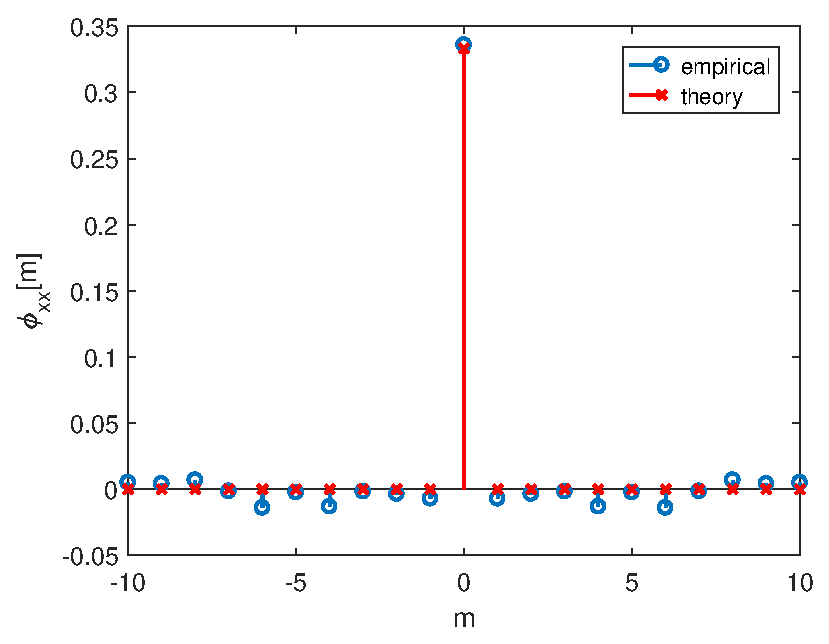
\includegraphics[width=\linewidth]{figs/lec2_random_experiment1_phi_xx.eps}
		\end{figure}
	}
	\only<3|handout:2>{
		\begin{figure}
			\centering
			\includegraphics[width=\linewidth]{figs/lec2_random_experiment2_phi_xx.eps}
		\end{figure}
	}
	\end{column}

	\begin{column}{0.5\textwidth}
		\only<2|handout:1>{
		\begin{figure}
			\centering
			\includegraphics[width=\linewidth]{figs/lec2_random_experiment1_phi_yy.eps}
		\end{figure}
		}
		\only<3|handout:2>{
			\begin{figure}
				\centering
				\includegraphics[width=\linewidth]{figs/lec2_random_experiment2_phi_yy.eps}
			\end{figure}
		}
	\end{column}
\end{columns}
\onslide<3|handout:2>{Now the random vector is $10000\times 1$}
\end{frame}

\begin{frame}{Estimating the probability density function}
\texttt{>> Nbins = 20} \\
\texttt{>> [counts, centers] = \textbf{hist}(x, Nbins)} \\
{\color{matlabcomment}\% normalize to make area under pdf equal to 1} \\
\texttt{>> x\_pdf = Nbins/(centers(end) - centers(1))*counts/sum(counts)} \\
\texttt{>> bar(centers, x\_pdf) {\color{matlabcomment}\% plot}}
\begin{columns}
	\begin{column}{0.5\textwidth}
			\begin{figure}
				\centering
				$p_x(x)$
				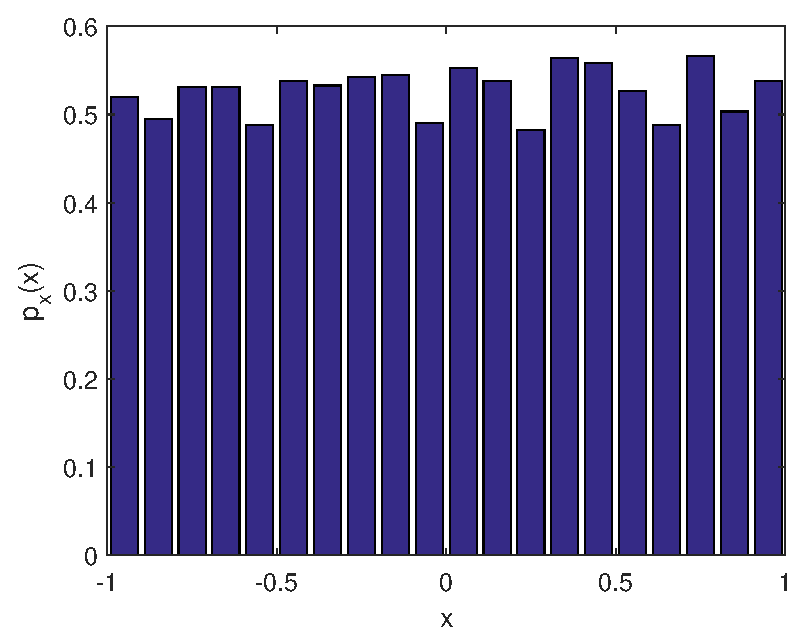
\includegraphics[width=\linewidth]{figs/lec2_random_experiment1_hist_x.eps}
			\end{figure}		
	\end{column}
	\begin{column}{0.5\textwidth}
	\begin{figure}
		\centering
		$p_y(y)$
		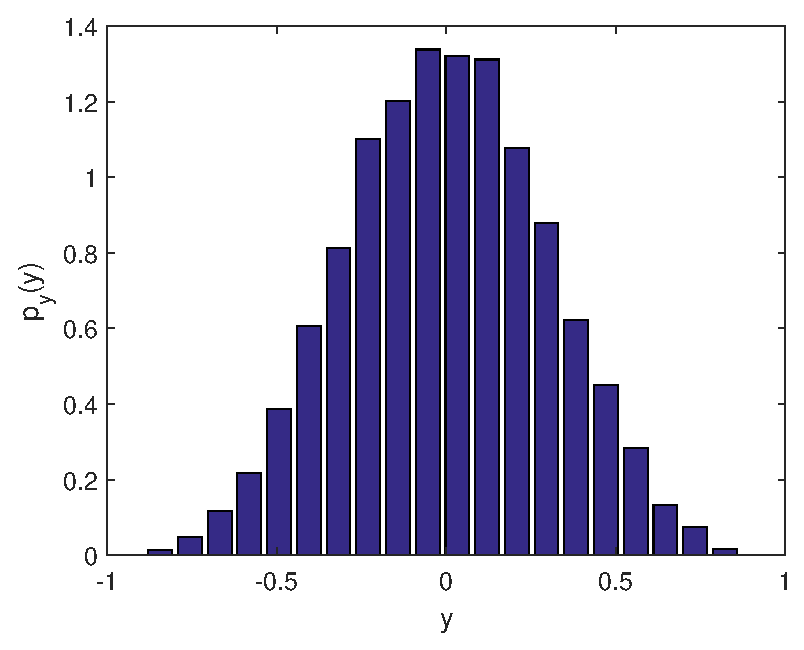
\includegraphics[width=\linewidth]{figs/lec2_random_experiment1_hist_y.eps}
	\end{figure}		
\end{column}
\end{columns}
\end{frame}

\begin{frame}{Central limit theorem}
The \textbf{central limit theorem} states that the probability density function of the sum of a large number of independent random variables approaches a Gaussian distribution.
\begin{equation*}
Z = X_1 + X_2 + \ldots + X_N \implies p_Z(z) \to\mathcal{N}(\mu, \sigma^2)
\end{equation*}

\begin{itemize}
	\item In digital filters, we're essentially performing a weighted sum of samples of the input. As a result, the output of a digital filter for a random input is approximately Gaussian distribution.
	\item In the example of the 4-point moving average system, we were only adding 4 random variables and the resulting output pdf was close to Gaussian. 
	\item This effect is more visible in filters with larger memory, and in particular in filters with \textbf{infinite impulse response (IIR)} 
\end{itemize}

\end{frame}

\begin{frame}{Another probability theorem}

If we add two independent random variables $Z = X + Y$, the pdf of $Z$ is given by the convolution of the pdfs of $X$ and $Y$

\begin{equation*}
p_Z = p_X \ast p_Y
\end{equation*}

\pause
We can extend that to a sum of several independent random variables:
\begin{equation*}
Z = \sum_{k=1}^N X_k \implies p_Z = p_{X_1} \ast \ldots \ast p_{X_N}
\end{equation*}

\pause
From the \textbf{central limit theorem}, we know that as $N\to\infty$,  $p_Z\to\mathcal{N}(\mu, \sigma^2)$

\begin{itemize}
	\item This shows that the convolution of many signals $h_1(t) \ast h_2(t) \ast \ldots \ast h_N(t) \approx g(t)$, where $g(t)$ is the Gaussian function.
	\item Hence, if we cascade many LTI systems, the impulse response of the equivalent LTI system is approximately the Gaussian function.
\end{itemize}


\end{frame}

\begin{frame}{Summary}
\begin{itemize}
	%\item We use random processes to model signals that cannot be easily described by simple equations
	\item A random process is an indexed collection of random variables
	\item A random process is strict-sense stationary (SSS) if all its finite-order statistics are time invariant. That's hard to verify in practice.
	\item A random process is wide-sense stationary (WSS) if its mean is constant and if its autocorrelation function is only a function of the time difference. 
	\item A random process is ergodic if its time averages are equal to its probability averages
	\item The Fourier transform of the autocorrelation function is called the power spectrum density (PSD). The PSD has units of W/Hz or dBm/Hz.
	\item When a random signal is filtered by an LTI system defined by $h[n]\leftrightarrow H(e^j\omega)$, its autocorrelation function is filtered by an LTI system defined by $h[n]\ast h^*[-n]$, and its PSD is shaped by $|H(e^{j\omega})|^2$
	\item Random processes that have PSD constant over all frequencies are called white noise
	\item By the central limit theorem, the output of an LTI system to a random input is approximately Gaussian distributed
	
\end{itemize}
\end{frame}

\end{document}
